\chapter{Centrality measures}
\label{chap:Centrality measures}



 \begin{displayquote}
 I asked a person of intelligence how many steps he thought it would take, and he said that it would require 100 intermediate persons, or more, to move from Nebraska to Sharon. \cite{milgram1967small}
 
 Stanley Milgram 1969
\end{displayquote}



The post synaptic proteome network (PSP - section ) and population samples ( section) are used in this chapter to test the hypothesis that important synaptic proteome nodes are more likely to be associated with genetic variants linked to differences in intelligence or educational attainment. The reasoning being that effects on critical nodes will disproportionately affect the function of the (nervous) system. 

Networks can be studied at three levels: the properties of the network as a whole, such as the small-world property (section~\ref{sec:Small world}), the properties of individual nodes including their importance to the network, and finally the analysis of meso-scale structures found within the network such as communities (chapter~\ref{chap:community detection}).
  
  The principle node properties are measures of \textit{centrality}.The concept of centrality arose in the social sciences literature in the late 1940s and its early evolution is reviewed in Freeman \cite{freeman1978centrality}. Centrality measures use network topology to determine how important nodes are\cite{newman2018networks} and their relative position (central or peripheral) within the network \cite{freeman1978centrality}.

 In real world networks a small number of nodes are often critical to network function, for example a hub airport in an air transportation network\cite{borenstein1989hubs}\todo{check this ref is 1989}. Centrality statistics measure the different ways in which nodes can be important in a network allowing key nodes to be identified, ranked and any association between centrality and network function assessed. 
 
Genes that encode proteins that are central in the proteome have been shown to be vital, most famously mutations in hub (high degree centrality) genes in the yeast proteome are more likely to be lethal (the \textit{centrality lethality} effect)\cite{jeong2001lethality}; central genes have also been reported to be more commonly associated with some diseases most notably cancer\cite{vogelstein2000surfing}, \cite{albert2005scale},\cite{xu2006discovering} although the relationship is complex and recent results question even the previously accepted degree centrality effects in yeast (section~\ref{sec:biomedical significance of centrality measures}).

Before addressing the association between synaptic proteome centrality and cognition, it is necessary to introduce these centrality measures, briefly review their previous use in the biomedical literature and their effects on the function of the network. We will then be able to see what roles genes associated with animal models of molecular cognition have in the network and compare these with the network topology of significant variants in the genetic population GWA studies of cognitive ability and educational attainment.   


 
Given the importance of the synapse in cognition, important nodes in the synaptic proteome network might disproportionately affect animal models of cognition or human differences in intelligence. There is evidence that central nodes affect numerous genes and in a protein network impact \textit{pleiotropic} traits and diseases \cite{chavali2010network} and Intelligence has a pleiotropic genetic architecture\todo{omnigenic model}\cite{plomin2015genetics},\cite{visscher2016plethora}.  Conversely there may be no effect; genetic variation in critical nodes may be so deleterious as to be  lethal or cause levels of impairment that would absent sufferers from large scale genetic studies of cognitive ability. Central genes have been reported to be essential rather than associated with disease\cite{barabasi2011network} although the definition of variations in disease and of disease genes varies (see section \ref{sec:assessment of communities}) in a way in which has not always been recognised in the literature (for an example see \cite{goh2007human} in the discussion).
\footnote{\url{\footnote{(Degree 1:304, Degree 2:293, 3:248 4:245 5:188 6:167)}}}
 What is therefore needed is an empirical approach to study the effects of network topology on complex traits and diseases and an appreciation that effects may be specific to only some traits or diseases. Also like the quotation that starts this chapter we should keep in mind our original intuition about what the findings might be.
 
 
 
 

 


\section{Properties of `real world' networks}
\label{sec:Properties of empirical networks}
Real world  networks often have properties that would not be expected to arise by chance. These include: a power law degree distribution \cite{barabasi1999emergence},\cite{barabasi1999mean} (section~\ref{sec:scale_free}) and `small world' structure \cite{watts1998collective}. Network level properties in turn arise from the collective properties of individual nodes; for example a degree sequence (node level) gives rise to a power law distribution (network level) or individual local transitivity to global clustering coefficient\cite{watts1998collective}. In addition to centrality measures (section~\ref{sec:centrality measures}) nodes may have properties including  non-topological node data\cite{wang2016approach} or metadata\cite{peel2017ground} of which the gene level significance scores from GWAS studies are an example. Chapter~\ref{chap:community detection} will address meso-scale structures and community detection. 

Network level statistics reflect how networks form and evolve, their patterns of information flow and how resistant they are to disruption. Not all naturally occurring networks share the same network level properties; for example, road networks do not show a scale free property\cite{xie2007measuring}\footnote{their degree distribution is similar to that found in a random graph} although air travel networks do\cite{boccaletti2006complex}\footnote{to be more accurate we might say do not belong to a heavily right skewed distribution}.The presence and magnitude of these properties can be determined by seeing how a network differs from a completely random model or a model in which some of its features, such as degree distribution (section \ref{sec:degree distribution}), are kept fixed. 





\todo{ref}
\todo{note trying to say network level statistics tell us things like }




\todo{?add global graph measures}

\subsection{Small world property}
\label{sec:Small world}
% \textcolor{red}{this is not covered in introduction}
The `small world' property means that any node in the network can be reached by a short number of hops along edges from any another node. The maximum distance, the \textit{diameter D}, between any two nodes in the network is small\cite{zhu2007getting}. It has recently been posited as the mechanism of an `omnigenic' model of traits \cite{boyle2017expanded}. Random networks are small but their nodes do not tend to cluster together. 

The phenomena was memorably demonstrated by Milgram\cite{milgram1967small}\footnote{although it was previously described see Newman \cite{newman2018networks}
p 62 citing Pool and Kochen a\footnote{\url{\footnote{(Degree 1:304, Degree 2:293, 3:248 4:245 5:188 6:167)}}}lthough published later \cite{de1978contacts} }. In his 1967 experiment he attempted to determine the number of steps that it would take for a letter to reach a recipient unknown to the first letter holder if they could only mail it to people known personally to themselves (the average path length). The average number of links was six, contrary to his expectations\footnote{Milgram reports it as the median number of intermediaries as five, which is six edges between sender and recipient using the definition of path length} \footnote{? remove This resulted in the title of the popular play by John Guare}. 

Watts and Strogatz \cite{watts1998collective} reported small world properties in naturally occurring networks: the neural network of the nematode \textit{Canenorhabditis elegans}; the power network of the western United States, and the collaboration graph of film actors generated from the Internet Movie Database (IMDb). These properties are: a short average path length, with a high clustering coefficient compared with a random graph\footnote{small path length but small clustering coefficient}. The average path length of small world networks and ER networks are proportional to the logarithm of the number of nodes in the network. Scale free networks scale as loglogN\cite{cohen2003scale}.\footnote{scales as loglogN in scale free with core periphery \cite{boccaletti2006complex}}. 

Watts and Strogatz\cite{watts1998collective} proposed a generative model for this phenomenon where\cite{newman2018networks}\footnote{p312} a circular lattice network has edges rewired randomly with probability $p$ in which interconnections are rewired to span the circle. A small amount of rewiring allows a short path length and preserves the high clustering coefficient. Figure~\ref{fig:small_world} shows the generation of a small world graph from a circular lattice with increasing rewiring probability.

Only a small number of edges need to be rewired to produce the small world property and this has been proposed as a significant reason that it is common in nature \cite{newman2018networks}\todo{ref}. Small world networks in the Watts-Strogatz model (WS) are a stage between random networks and lattices and it has also been suggested that their ubiquity may be related to the advantageous combination of clustering and connectivity\cite{latora2001efficient}.

The small world property allows rapid information transfer within networks. It has recently been posited as a model for wide spread genetic effects on traits (the omnigenic model)\cite{boyle2017expanded}\footnote{however see also \cite{wray2018common} for a non network criticism and see discussion}, and as a developmental stage in the evolution of brain networks\cite{vertes2015annual}. For results see section~\ref{sec:Results average path length and transitivity}




\begin{figure}
    \centering
    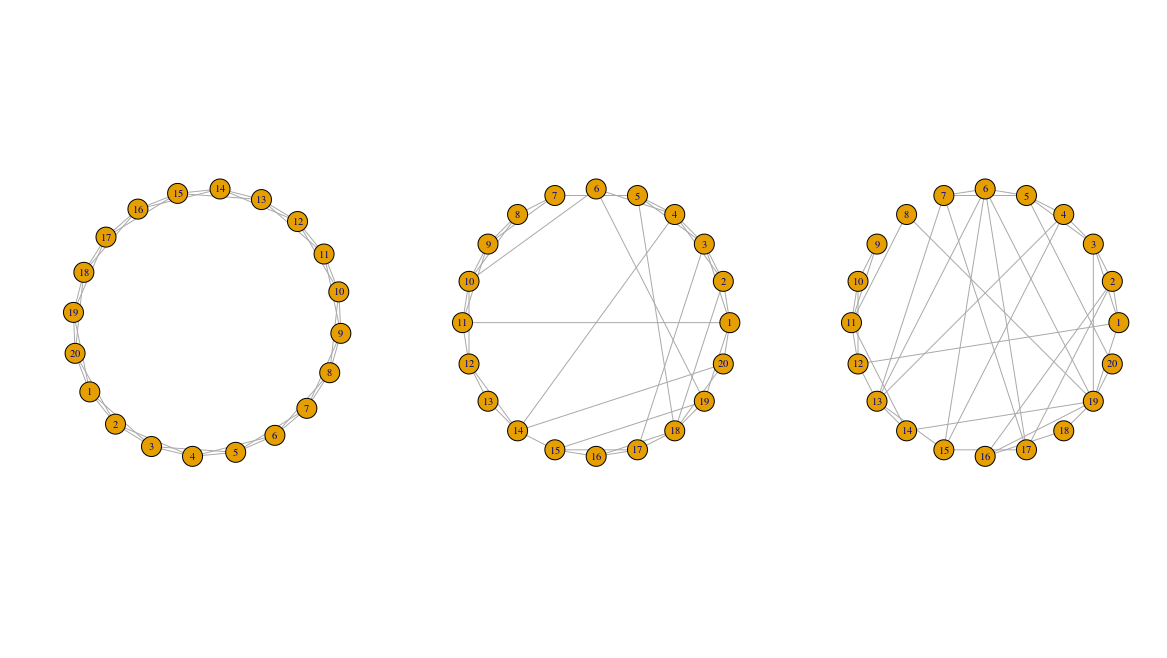
\includegraphics[width=\textwidth]{images/Rplot_corrected_small_world.png}
    \caption{Small world lattice n=20. p of rewiring = 0,0.1,0.3. Code at \url{source('~/RProjects/graph_sw/R/plot_small_world/plot_small_world.R')}.\textcolor{red}{ADD APL and transitivity below each plot}}
    \label{fig:small_world}
\end{figure}

\todo{small world network either do here or put in introduction this goes with results }

 

\subsection{The configuration model}
\label{sec:configuration model}

To assess the significance of a network or a vertex statistic we can measure how much they differ from their expected value given a random network. Simple random networks such as Erd\H{o}s-R\'enyi (ER) random graphs have already been introduced (see section~\ref{sec: PSP graph connected component and missing}).

Erd\H{o}s-R\'enyi models generate networks with a vertex degree distribution that is approximated by a Poisson distribution (see section~\ref{sec:degree distribution}) and hence with the mode of the probability mass centred around the mean degree $<k>$ of the network\todo{move this to after degree distribution}. Many real world networks have more complicated degree structures, often a heavy tailed distribution such as a power law distribution (section~\ref{sec:scale_free}).

The configuration model generates a new random network that retains the degree sequence of the original network. Network properties can therefore be compared between the real network and a configuration model with identical degree sequence which allows random models to be generated of networks with arbitrary degree structures. The process for generating the configuration model is as follows: each edge is broken into two stumps and then each of the stumps are rewired in turn into another stump with a uniform probability\todo{add image}. This can result in self loops and multiedges\footnote{check how multiedges is written in newmanDONE it is multiedges}, which do not occur in most real world networks, but the number of these are low as the network size increases \cite{newman2018networks}.

There are alternate, specific models for generating random power law distribution networks such as the Barabasi-Albert model\cite{barabasi1999emergence} and earlier Price model\cite{price1965networks}.
If studying a \textit{particular} network for which one has the degree sequence, as is the case here, the configuration model is a good choice\todo{rephrase}\cite{newman2018networks}.

\begin{figure}
  \begin{subfigure}{7cm}
    \centering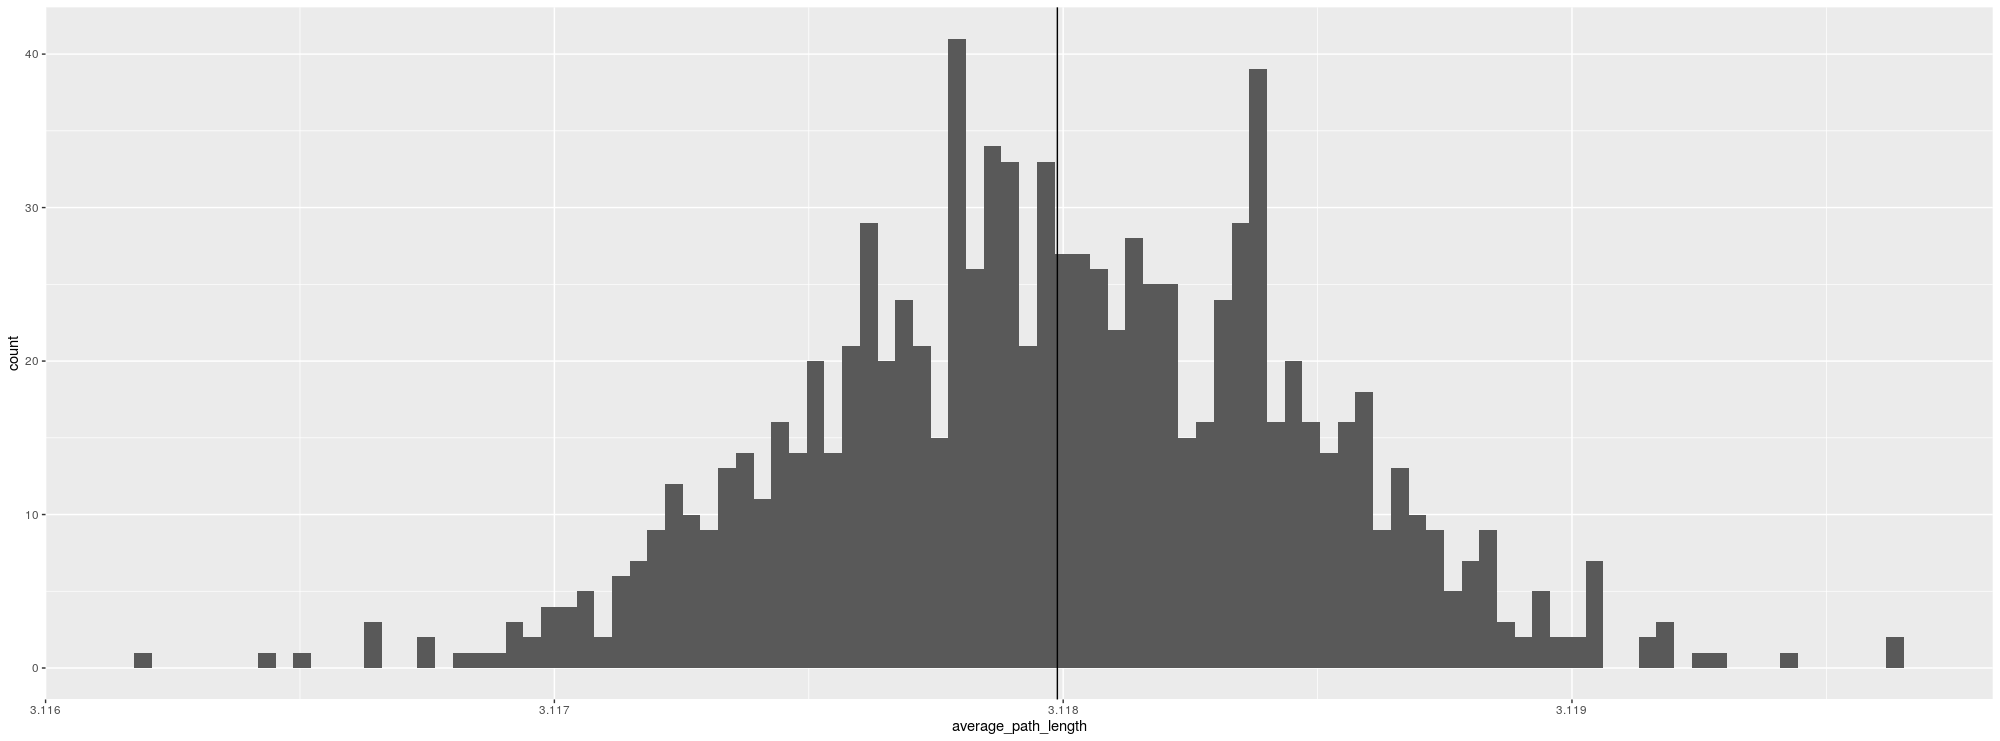
\includegraphics[width=7cm]{images/chapter3/small_world_histogram/Rplot_average_path_length.png}
    \caption{Average path length}
    \end{subfigure}
  \begin{subfigure}{7cm}
    \centering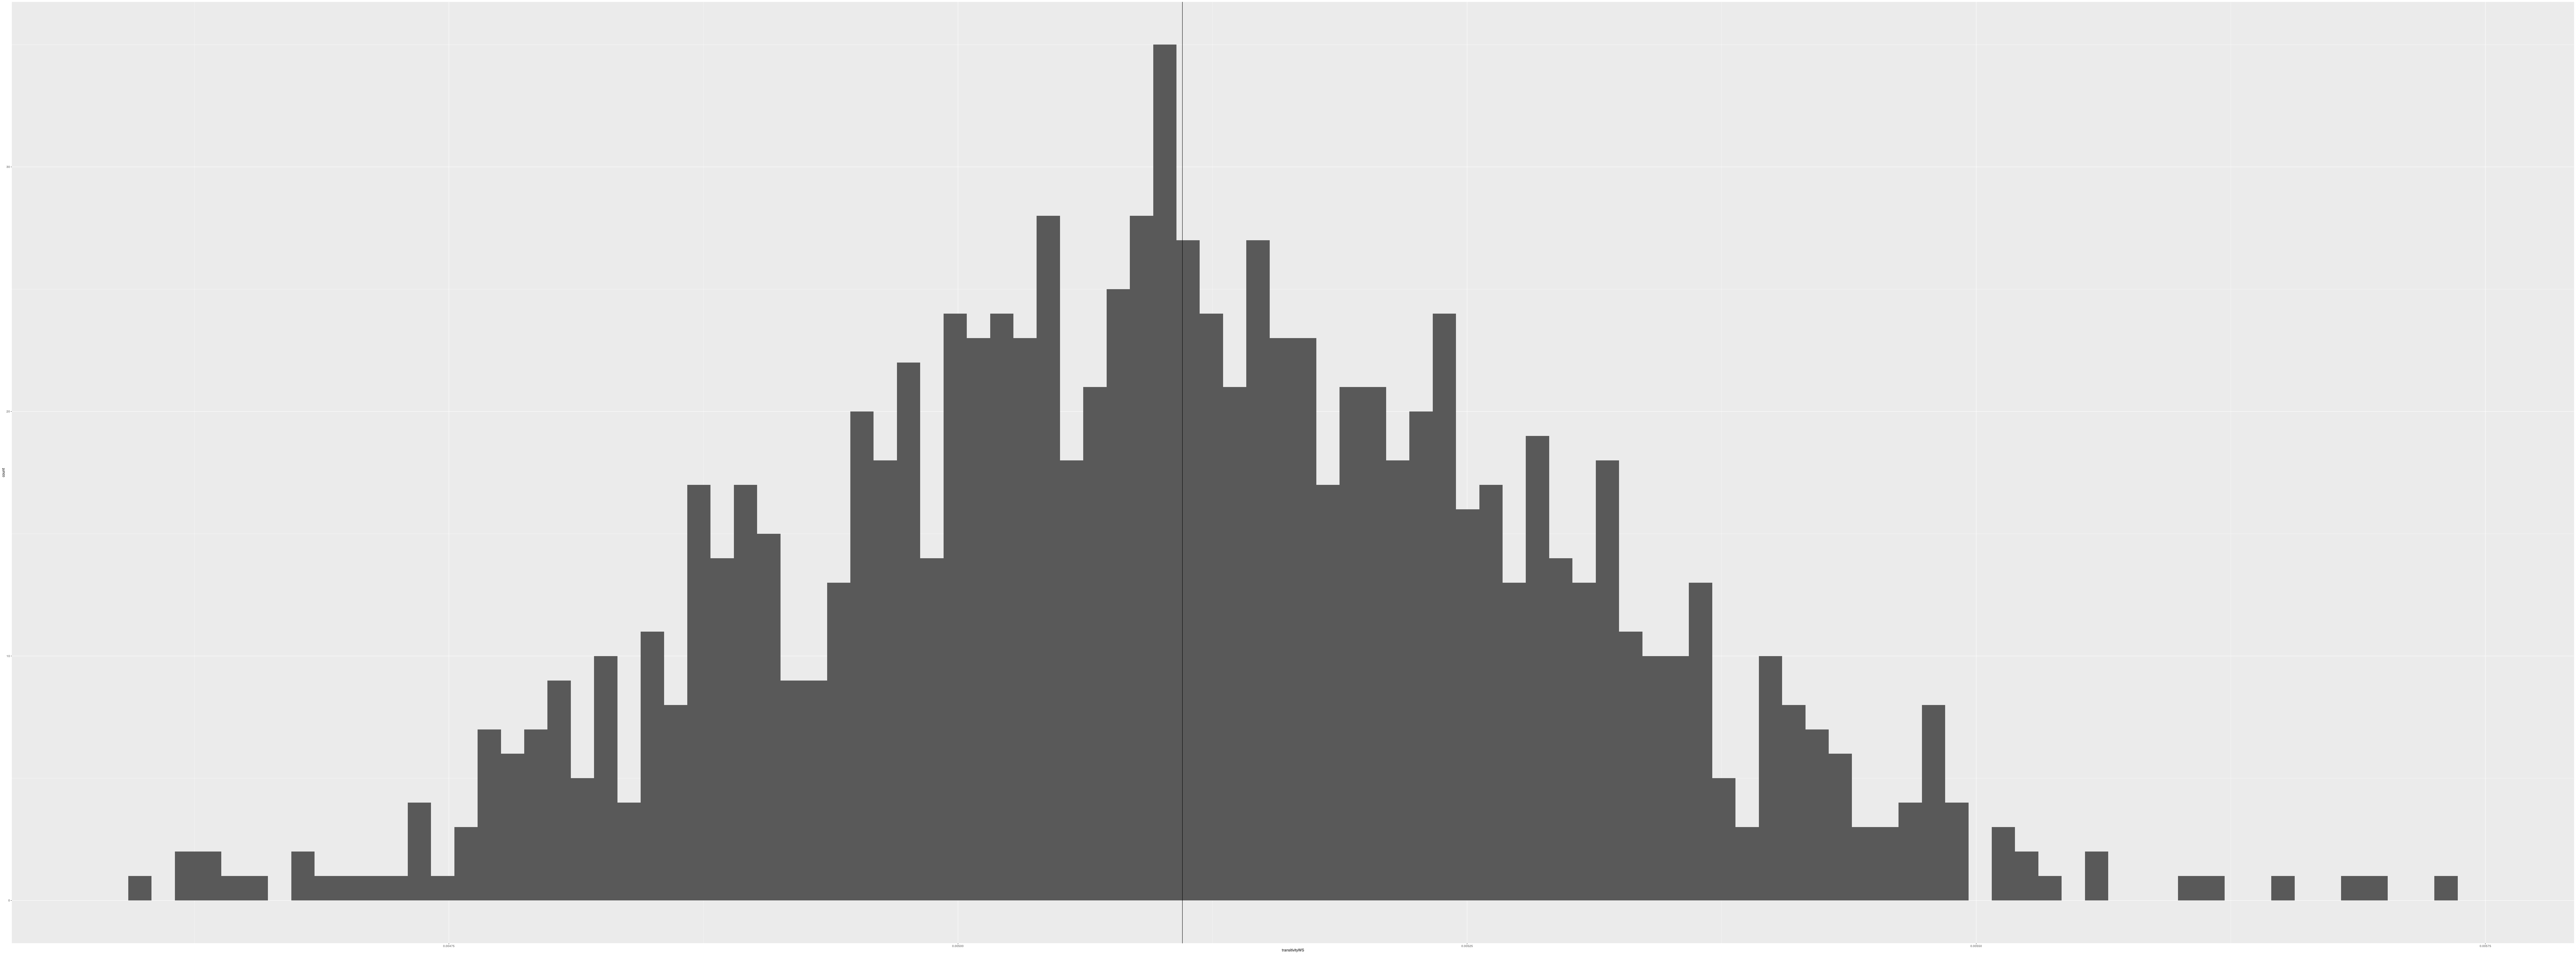
\includegraphics[width=7cm]{images/chapter3/small_world_histogram/Rplot_transitivityWS_ER_graph3457.png}
    \caption{Transitivity Watt Strogatz.}
  \end{subfigure}

 
 \begin{subfigure}{7cm}
    \centering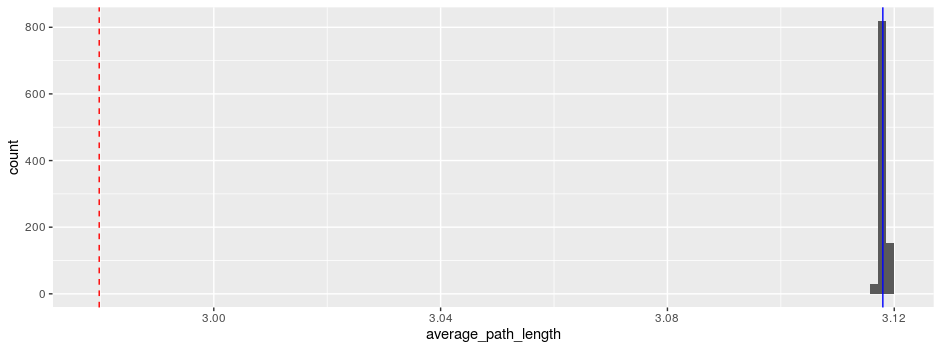
\includegraphics[width=7cm]{images/chapter3/small_world_histogram/Rplot_average_pathlmean.png}
    \caption{Average path length showing mean}
    \end{subfigure}
  \begin{subfigure}{7cm}
    \centering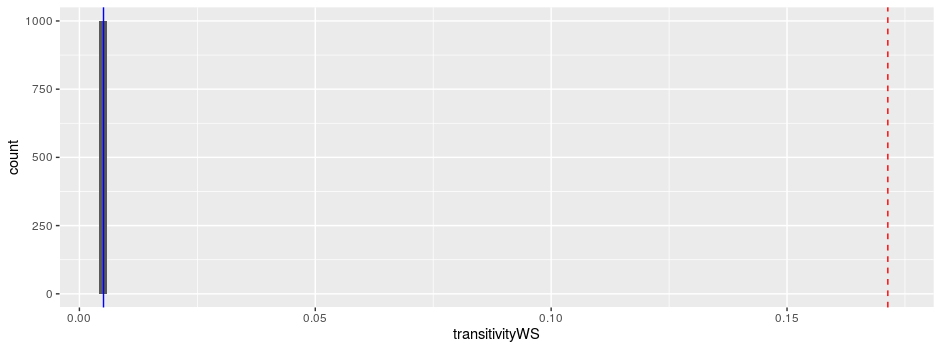
\includegraphics[width=7cm]{images/chapter3/small_world_histogram/Rplot_transitivity_mean.png}
    \caption{Transitivity Watt Strogatz.}
  \end{subfigure}
\caption{Figure shows average path length and transitivity (Watts Strogatz mean of local transitivity) for an Erdos Renyi graph of 3457 nodes and 30498 edges (i.e. the same as the PSP graph). The difference in values is small but the sampling distributions do not overlap. Upper panels show the distribution of these values over 1000 iterations \url{source('~/RProjects/chapter3/R/small_world/eda_small_world.R')}}
 
  \end{figure}

\section{Centrality measures}
\label{sec:centrality measures}
Centrality measures identify important, central nodes in a network \cite{newman2018networks}\footnote{(p159)} based on network topology. This can also be interpreted as a measure of how information flows through a network \cite{borgatti2005centrality} and a variety of measures of importance have been described (see section~\ref{sec: intro_centrality_measures}). These are measures of individual vertices and can therefore be used to rank, group or identify key nodes. All measures are derived from the adjacency matrix\footnote{references for what are 'classic' measures vary \cite{cadini2008using} has closeness, betweenness, information and degree but not eigenvector which most have there is another reference for this but I can't fint it at the moment}.

\begin{figure}
  \begin{subfigure}{7cm}
    \centering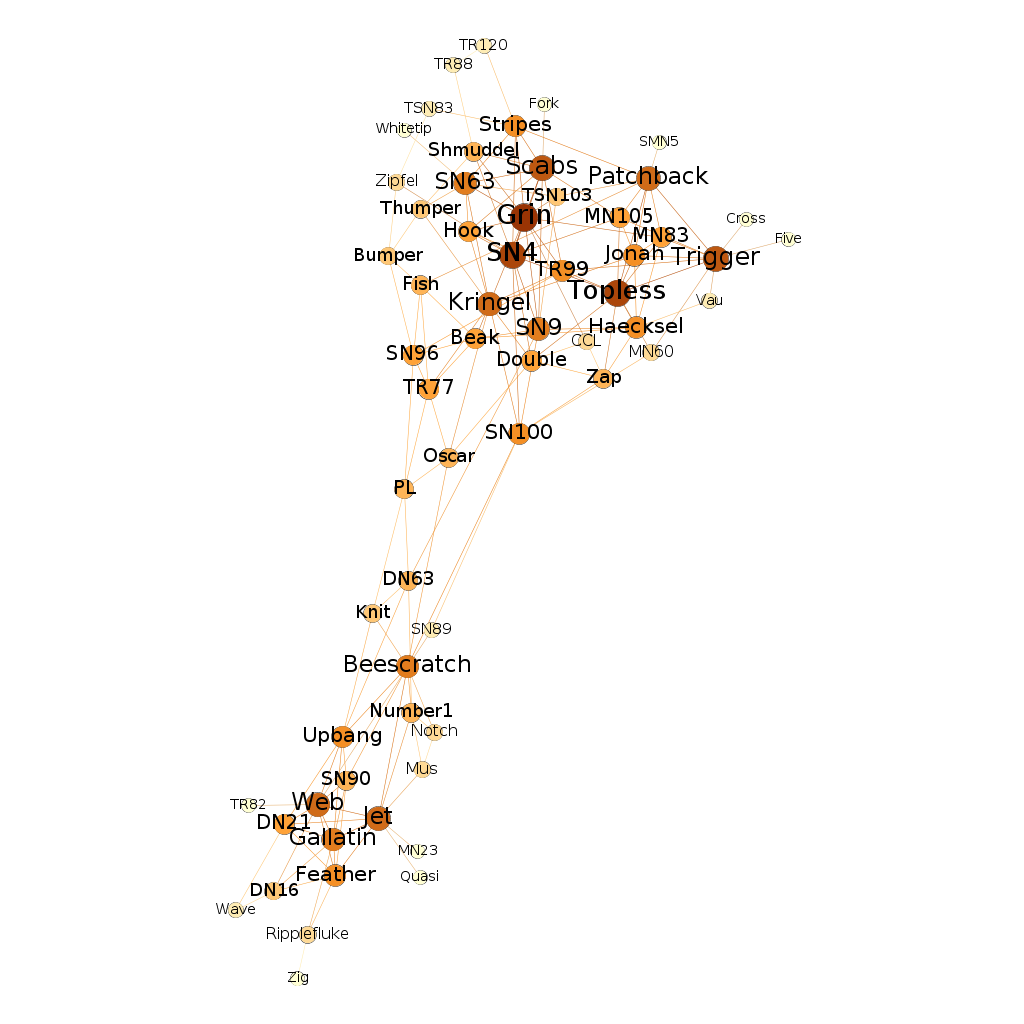
\includegraphics[width=7cm]{images/chapter3/dolphin/degree.png}
    \caption{Degree}
    \end{subfigure}
  \begin{subfigure}{7cm}
    \centering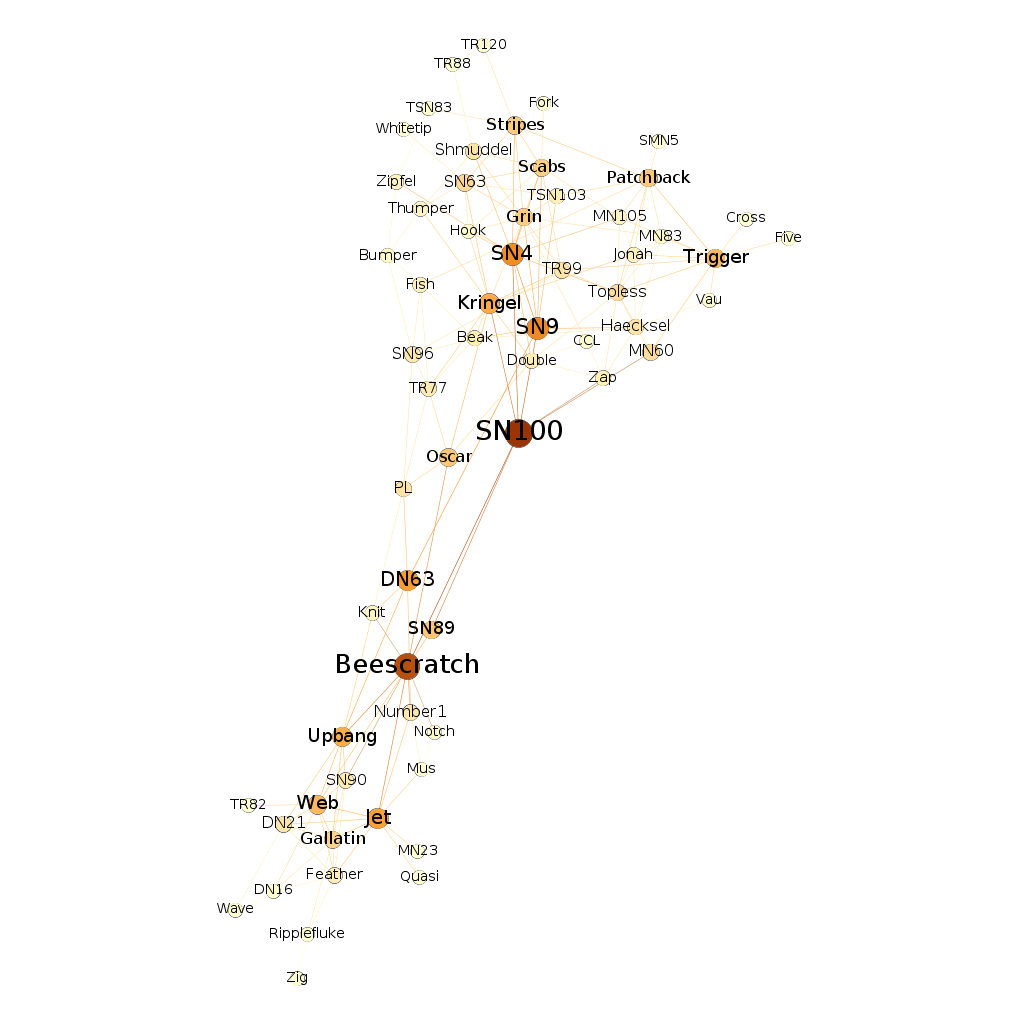
\includegraphics[width=7cm]{images/chapter3/dolphin/betweenness.png}
    \caption{Betweenness}
  \end{subfigure}
  \begin{subfigure}{7cm}
    \centering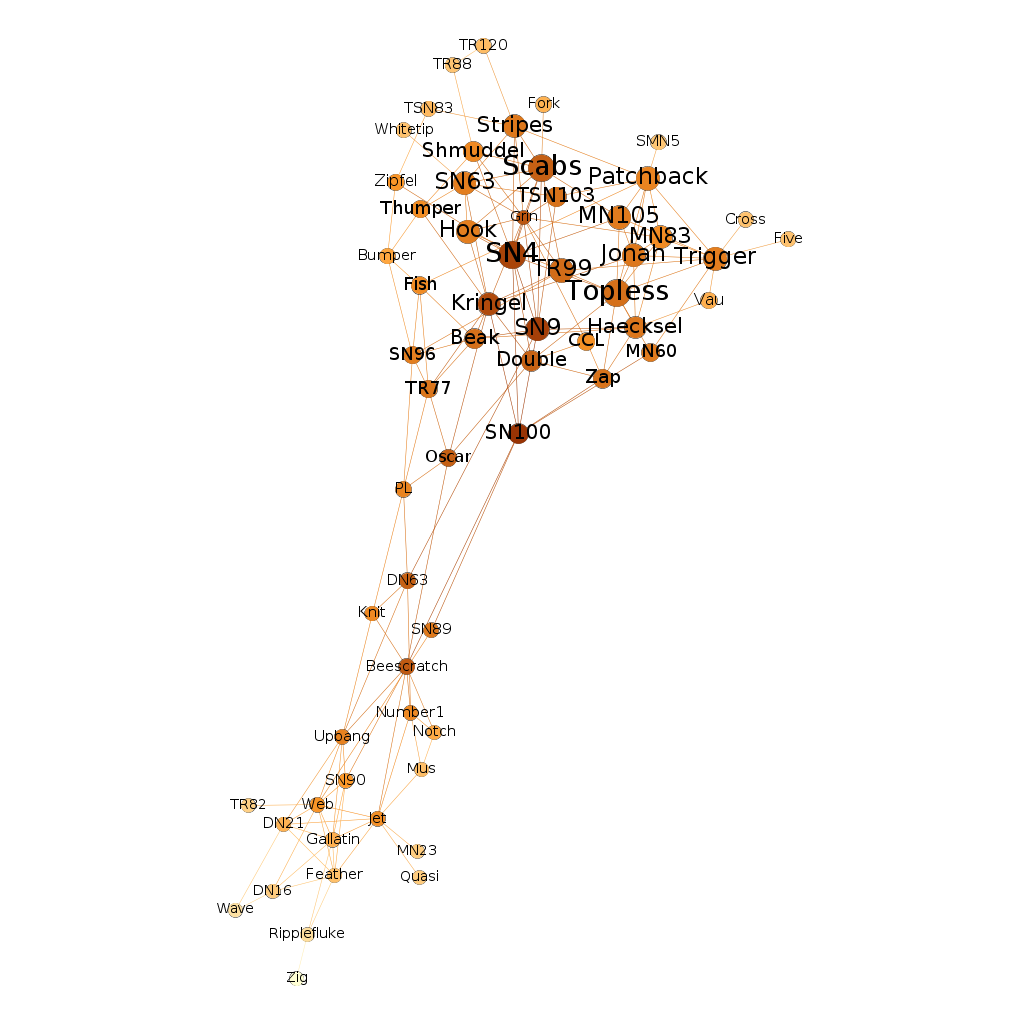
\includegraphics[width=7cm]{images/chapter3/dolphin/closeness.png}
    \caption{Closeness}
  \end{subfigure}
  \begin{subfigure}{7cm}
    \centering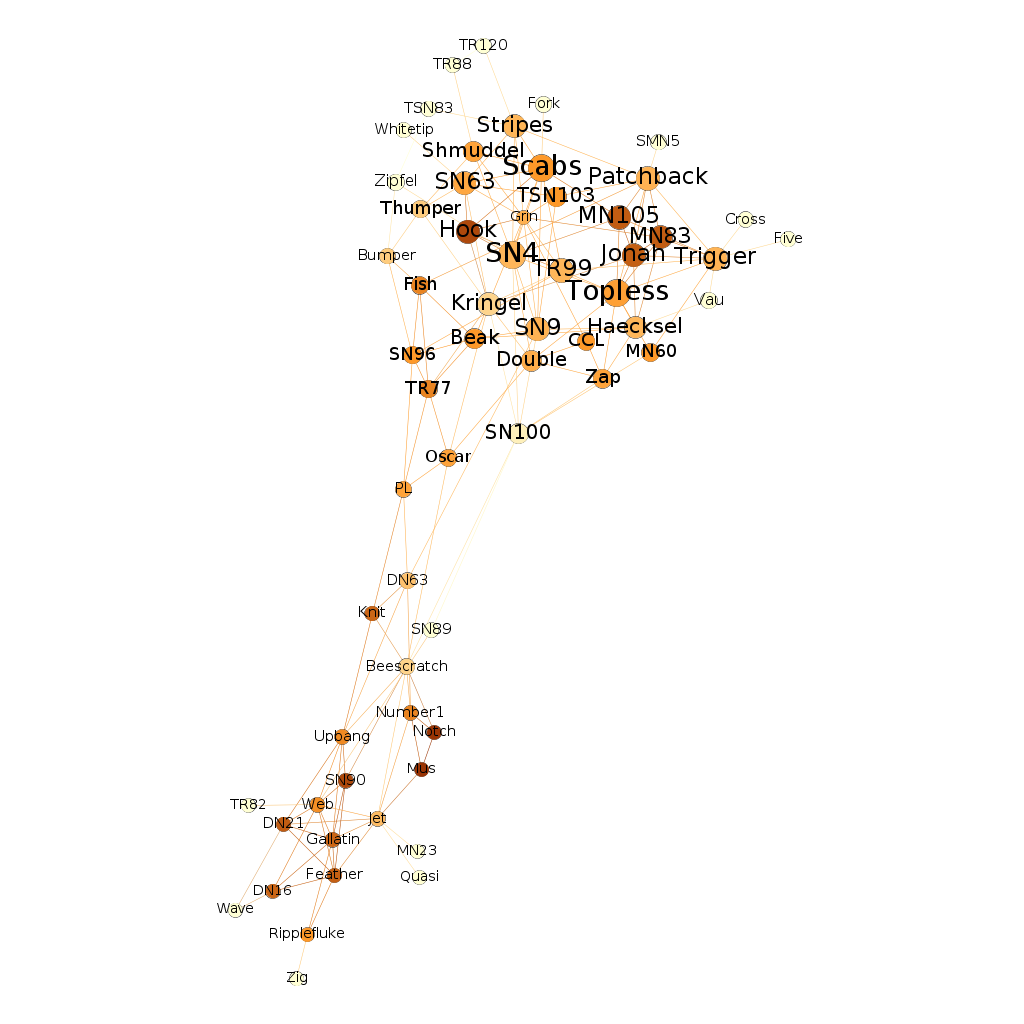
\includegraphics[width=7cm]{images/chapter3/dolphin/eig.png}
    \caption{Eigenvector}
  \end{subfigure}
  \caption[\textbf{Illustation of entrality measures} in a dolphin social network.]{Display of centrality measures. Betweenness centrality, eigenvector centrality and local transitivity for a social network of bottle nose dolphin social relations data. Node size is proportional to centrality measure and node colour varies from pale yellow (low) to red (high centrality). Dolphin names are shown in the text and the font size is also proportional to centrality measure. Note that the betweenness shows two prominent nodes SN100 and Beescratch through whom many shortest paths flow although they have modest degree centrality and eigenvector centrality. Hook, is a neighbour of a number of high degree nodes but has a modest degree centrality shown in a). The importance of Hook's connections is shown in the high eigenvector centrality in panel (d). Data from Prof Newman's website\footnote{\url{http://www-personal.umich.edu/~mejn/netdata/dolphins.zip}} based on Lusseau et al. (2003) \cite{lusseau2003bottlenose}.Visualisation in Gephi with Force Atlas layout. }
  \label{fig:dolphin_multipanel}
\end{figure}
\begin{figure}
    \centering
    \includegraphics[width=0.9\textwidth]{images/chapter3/centality_plos/journal.pone.0220061.g001.PNG}
    \caption{Centrality measures from Oldham et al. (2019)\cite{oldham2019consistency}. In panel A the red node has both high degree and closeness. In contrast in panel B the red node has high centrality but low degree. This image illustrates that although these measures can be correlated they can also represent different properties.}
    \label{fig:centrality measures from Plos}
\end{figure}

Degree centrality is the most familiar and simplest equal to the number of edges that a vertex is incident to. Other vertex measures include eigenvector centrality, a measure of the importance of the node that includes the degree of its neighbours\cite{bonacich1987power}.  Some nodes are bottlenecks in the network. If a large number of the shortest (geodesic) paths pass through a node it is a potential bottleneck and its removal can disrupt the integrity of the network. The measure of a nodes propensity to be a bottleneck is the betweenness centrality\cite{freeman1977set}. Closeness centrality measures how close a vertex is on average to all other nodes in the network. Transitivity, though not a classic centrality measure, can be seen as a local form of betweenness centrality \cite{newman2018networks}. In this section I include transitivity and kcoreness as  measures of importance of a node. They are often considered in contexts other than centrality but do provide a method to rank the importance of the node and its effect on others, which is key to the concept of centrality. They are also correlated with the other measures and some of these correlations are of interest, therefore it seems reasonable to present them is along with the centrality measures.

 Centrality measures are frequently correlated with each other \cite{valente2008correlated} although their correlation varies\cite{oldham2019consistency}. Figure~\ref{fig:dolphin_multipanel} shows vertex degree, betweenness centrality, closeness and eigenvector centrality in a real world network, a social network of bottle nose dolphins \footnote{\url{http://www-personal.umich.edu/~mejn/netdata/dolphins.zip}} \cite{lusseau2003bottlenose}. High values of these measures are shown in red. 

Figure~\ref{fig:centrality measures from Plos} shows the fact that centrality measures can be concordant (for example high degree and closeness in panel a) or discordant (red node has high centrality and betweenness in panel b but low degree). Over 200 centrality measures have been described \cite{jalili2015centiserver}. Many are correlated \cite{valente2008correlated} and different patterns of correlation have been reported recently in different networks \cite{oldham2019consistency}. 

% \begin{figure}
%     \centering
%     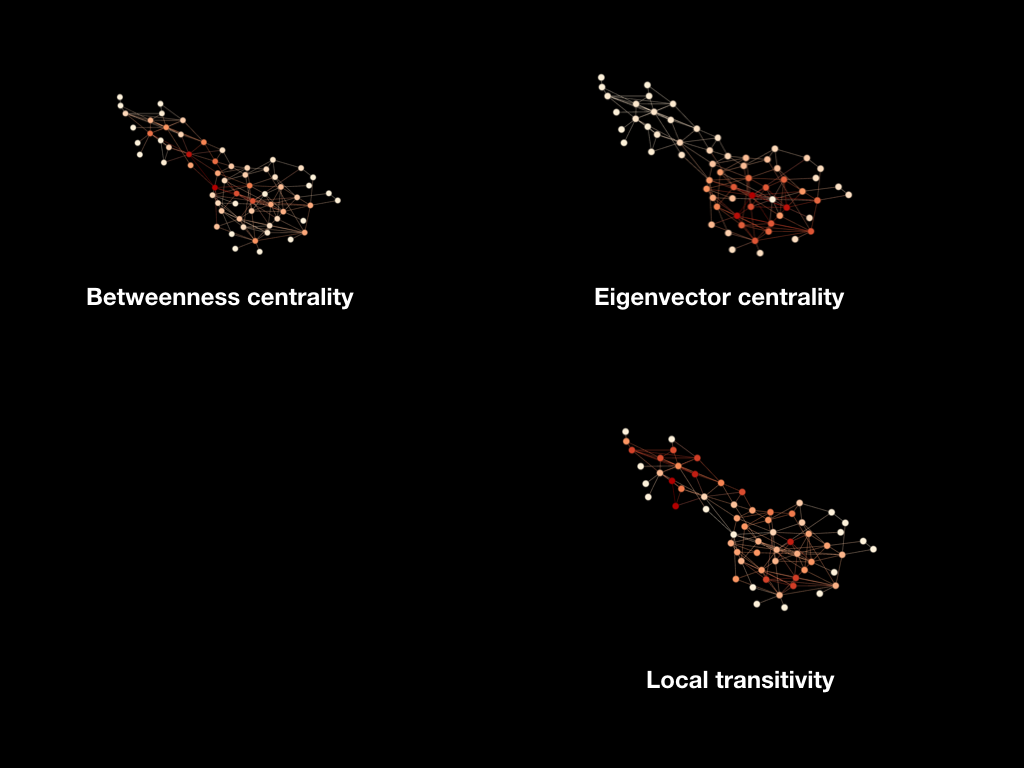
\includegraphics[width=0.9\textwidth]{images/centrality2002.png}
%     \caption{Display of centrality measures. Betweenness centrality, eigenvector centrality and local transitivity for network of bottle nose dolphin social relations data. \cite{lusseau2003bottlenose}}
%     \label{fig:dolphin}
% \end{figure}






This chapter will consider degree centrality, eigenvector centrality, betweenness, closeness and transitivity in the PSP and their association with animal models of learning and human cognitive ability. The six measures primarily used in this thesis have been those that are implemented in igraph and are sufficiently popular to appear in a general textbook\cite{newman2018networks}. Degree centrality and eigenvector centrality are neighbourhood based centrality measures, and closeness and betweenness shortest path-related\cite{kardos2020stability}\todo{find ref on what are the key centrality measures ?consistency and differences between centrality measures across distinct classes of network - this is on p3 of the Kardos ref \cite{kardos2020stability} and is degree, eig, closeness between and pagerank}. The simplest centrality measure, degree centrality, \cite{newman2018networks} is considered below. 

\subsection{Degree centrality}
\label{sec:degree centrality}

%from \url{/home/grant/Dropbox/PhD_latex_master}
The degree of a node is the number of edges connected to it. A node that is connected to a large number of other nodes in a network may be influential in the network. In a protein interaction network changes in this protein may give rise to a variety of different phenotypes or if the protein is sufficiently essential, give rise to severe disease.  In the network graph of the PSP it is the number of proteins a protein (represented by its encoding gene) directly interact with.


All centrality measures can be derived from the adjacency matrix. The adjacency matrix $A_{i,j}$, represents an undirected, unweighted network such as the PSP,  where $A_{i,j}=1$  if there is an edge between nodes $i$ and $j$ and 0 otherwise, the degree of node $i$, $k_i$ is\cite{boccaletti2006complex}:
\begin{equation}
k_i = \sum_{j=1}^n A_{i,j}.
\label{Equation:Degree_from_adjacency}
\end{equation}

 Nodes with high degree may have more influence in a graph and are often referred to as `hubs'\cite{zhu2007getting}\footnote{In a directed network hubs may refer to nodes that point to authorities nodes with important information. As the post synaptic proteome network is undirected hubs will be used in the first sense in this thesis\cite{kleinberg1999authoritative}}.  In a social network individuals with a high degree centrality have many contacts and may therefore be influential in the network. In a protein-protein interaction network high degree proteins will have numerous interactions, take part in many biological processes and could therefore be an important part in the network. 
 
 Disruption of high degree nodes leads to disproportionate effects upon a network \cite{jeong2001lethality}, \cite{albert2000error}. Their effect on protein networks is reviewed by Zotenko\cite{zotenko2008hubs}.


\subsection{Degree distribution}
\label{sec:degree distribution}
The degree distribution of a network describes the probability, $p(k)$, that a  node has degree $k$. It is a probability distribution and so

\begin{equation}
    \sum_k p(k)=1.
\end{equation}

For an empirical network $P(k)$ is the number of nodes with degree $k$ divided by the number of vertices in the network. 

% An alternative representation for an emprical network is the degree sequence which is  node degree for each vertex in a network eg $1,1,2,3,5,7,\dots,n$. The properties of networks can be discovered by comparing these networks to random models (section~\ref{sec:configuration model}. It seemed reasonable that networks would have degree distributions similar to those found in Erdos Renyi graphs. It was only with the availability of information on large networks such as the internet and world wide web and computerised databases such as the IMDB that the fact that many natural networks have a power law distribution of node degree (section ~\ref{sec:scale_free}. Barabasi, Albert and Jeong found that the internet had a scale free distribution. A narrative of this discovery is provided in Network Science by Barabasi \cite{barabasi2016network}. 


If a graph were to have edges distributed between vertices with a uniform probability, $p$, we would expect the degree distribution ($P(k)=k)$) to be distributed according to the binomial distribution.  

 The probability of a node having $k$ links is $p^k$, the probability of there being no links to the remaining $N-1-k$ nodes (-1 as we exclude self loops) is $(1-p)^{N-1-k}$, there are $\binom{N-1}{k}$ ways in which this arrangement of present and missing edges can be arranged, so the degree distribution follows the binomial distribution\cite{barabasi2016network}:

\begin{equation}
   \binom{N-1}{k}        p^k (1-p)^{N-1-k}
   \label{Equation:BinomialDistributionForDegreeProbability}
\end{equation}

In the limit where the mean degree is much less than the number of nodes in the network the degree distribution is well approximated by a Poisson distribution \cite{barabasi2016network}. The Poisson distribution:

\begin{equation}
    p(k) = \frac{\lambda^k e ^-\lambda}{!k}
\end{equation}

has only one parameter for an empirical network, $E[k]$ which is $\lambda$.  The probability mass should be centred around the empirical mean  (17 in the case of the PSP). The variance of a Poisson distribution is $\lambda^{1/2}$ which is approximately 4.12. The top 20 post synaptic proteome genes (table~\ref{tab:The 20 post synaptic proteome genes with highest degree in their cognate proteins.}) have degree of 221 or greater. Under a Poisson model these are around 100 standard deviations greater than the mean.  \todo{probablility of max degree node} 
\todo{plot of Poisson and empirical for $E[k]$} \textcolor{red}{see figure}


\begin{table}[ht]
\centering
{
\begin{tabular}{@{}llll@{}}
  \toprule
Entrez ID &  $k$ & Symbol & Description \\ 
\midrule
351 & 535 & APP & amyloid beta precursor protein \\ 
  2335 & 474 & FN1 & fibronectin 1\footnote{Fibronectin lethality} \\ 
  1994 & 473 & ELAVL1 & ELAV like RNA binding protein 1 \\ 
  1956 & 450 & EGFR & epidermal growth factor receptor \\ 
  7514 & 396 & XPO1 & exportin 1 \\ 
  10482 & 375 & NXF1 & nuclear RNA export factor 1 \\ 
  7316 & 363 & UBC & ubiquitin C \\ 
  26270 & 342 & FBXO6 & F-box protein 6 \\ 
  7412 & 327 & VCAM1 & vascular cell adhesion molecule 1 \\ 
  55832 & 316 & CAND1 & cullin associated and neddylation dissociated 1 \\ 
  8454 & 316 & CUL1 & cullin 1 \\ 
  2885 & 313 & GRB2 & growth factor receptor bound protein 2 \\ 
  7534 & 298 & YWHAZ & tyrosine 3-monooxygenase tryptophan 5-monooxygenase \\
  3320 & 266 & HSP90AA1 & heat shock protein 90 alpha family class A member 1 \\ 
  10075 & 263 & HUWE1 & \makecell{HECT, UBA and WWE domain containing 1, E3 ubiquitin\\ protein ligase} \\ 
  4869 & 263 & NPM1 & nucleophosmin 1 \\ 
  7415 & 245 & VCP & valosin containing protein \\ 
  3178 & 227 & HNRNPA1 & heterogeneous nuclear ribonucleoprotein A1 \\ 
  22938 & 221 & SNW1 & SNW domain containing 1 \\ 
  8453 & 221 & CUL2 & cullin 2 \\ 
   \bottomrule
\end{tabular}
}
\caption{The 20 post synaptic proteome genes with highest degree in their cognate proteins.Degree $k$}  
\tiny Code to generate table at \url{source('~/RProjects/gridsearch_gamma/R/degree_distribution.R')}
\label{tab:The 20 post synaptic proteome genes with highest degree in their cognate proteins.}
\end{table}

\subsection{Scale free}
\label{sec:scale_free}
% \textcolor{red}{need to give background on barabasi etc}
% \todo{background scale free}
The work of Barabasi, Albert and Jeong (1999) led to the recognition that the degree distribution of nodes in real world networks is often scale free \cite{barabasi1999emergence},\cite{barabasi1999mean}\footnote{more recent work has suggested that scale free networks are relatively uncommon and that a log-normal or other distribution may be a better fit. When discussing the literature on scale free networks I have retained the use of scale free or power law from the original literature however it is understood that this includes the possibility of another significantly right skewed distribution}. In a scale free network the probability of a vertex having degree $k$, $p(k)$, is:

\begin{equation}
    p(k) \sim k^{-\gamma},
\end{equation}
\label{eq:scale free}

where $\gamma$ is the degree exponent\cite{barabasi2016network}.

Power law distributions are `scale free' because increasing the value of the degree changes the probability of the degree distribution by a common multiplicative factor. This results in a straight line graph on a log-log plot of degree $k$ and probability of degree $p(k)$, the signature of the scale free distribution\cite{beltrami2013mathematical}. 

Many other things in nature follow a scale free distribution (e.g. the size of craters on moon, frequency of words and size of cities) and subsequent research showed that many other networks (the first being the wiring diagram of an IBM chip, the map of the power grid and the Hollywood actor database) are all scale free\cite{barabasi2016network}. \footnote{ p11 in \cite{barabasi2016network}. Chapter 0 of this book gives a detailed personal history of the discovery of the scale free property in networks and its historical antecedents}

Albert, Jeong and Barabasi \cite{albert1999diameter} built a web robot to map out the links in the \url{nd.edu} domain of the world wide web. They found 325729 documents and 1469680 links. In  the world wide web documents point to other documents best represented by a directed graph. The network they constructed representing a sample of the world wide web displayed a power law distribution with $\gamma_{out}=2.45$ and $\gamma_{in}$=2.1. At that time (1998) there was `no trace in the literature of a network with a power-law distribution'\cite{barabasi2016network}\footnote{p10}.

The Barab\'asi-Albert model for generating a scale-free network distribution requires network growth and preferential attachment. Preferential attachment means that new nodes added to the network as it grows tend to be attached to nodes already of high degree\cite{barabasi1999emergence}.\todo{biology has active growth and also duplication} Price networks however had been described as a generative model for power law networks in the 1960s\cite{price1965networks}. 

The characterisation of power law distributions remains an active area of research in statistics. Many networks display the power law distribution only in the tails and some conform to log-normal distributions. Recent work has suggested that power law distributions are rare compared to other right skewed distributions\cite{broido2019scale}.  Despite this, the fact remains that many real world networks are right skewed with heavy tails and deviate markedly from a Poisson distribution. 




%%% CENTRALITY MEASURES %%%

\subsection{ Other centrality measures}

The previous section discussed the network level property of a scale free degree distribution along with the first centrality measure, degree centrality. 
\subsection{Betweenness centrality }
\label{sec:Betweeness centrality}
Betweenness centrality and closeness centrality (section~\ref{sec:closenesscentrality})  are both vertex centrality measures based on shortest paths between nodes\cite{newman2018networks}. Centrality measures can be considered Betweenness centrality, popularised by Freeman (1977) \cite{freeman1977set}\footnote{Newman \cite{newman2018networks} points out that Freeman acknowledges an earlier unpublished account by Anthosine}is a measure of the number of geodesic (shortest), paths in the network passing through a particular node. \textcolor{red}{define shortest path} 

 Following Newman's notation \cite{newman2018networks}, if $n_{st}^i=1$  if a shortest path between nodes $s$ and $t$ pass through node $i$ and  $g_{st}$ is the number of shortest paths between $s$ and $t$ (as there may be more than one shortest path) then the betweenness centrality of node $i$ is

\begin{equation}
    x_i = \sum_{st} \frac{n_{st}^i}{g_{st}}.
\end{equation}
\label{eq: Betweenness centrality}

In an undirected network, there is a shortest path in both directions between a pair of nodes e.g. from $s$ to $t$ and $t$ to $s$. This double counting does not alter the rank of the nodes ordered by betweenness centrality and allows for easier application to directed networks\cite{newman2018networks}. The betweenness centrality can be normalised by dividing by the number of possible node pairs in the network $n^2$ \cite{newman2018networks} \footnote{p176}.

Nodes with high betweenness centrality connect different areas on the network \todo{ref} (ie paths between nodes in the network disproportionately flow through them), and are sites of increased flow (of information for example). This assumes shortest paths are known and taken through the network \cite{borgatti2005centrality}  (random walk betweenness centrality measures betweenness when paths are random). Other nodes depend on nodes of high betweenness centrality and in the sociological literature they are sometimes referred to as `brokers'\cite{newman2018networks}. 



\subsubsection{Edge betweenness centrality}
 \todo{edge centrality}
 Edge betweenness centrality is the number of shortest paths that pass through a particular edge \cite{girvan2002community}.

\subsection{Random walk betweenness}
\label{sec: random walk betweenness}
The betweenness centrality described above assumes that information takes the shortest path through the network although this may not always be true. Random walk betweenness is a betweenness metric dependent on the property of random walks in the network. The results are often similar and where they differ it is not apparent what significant should be given to this difference\cite{newman2018networks}. For this reason I have not included random walk betweenness. 

\subsection{Closeness centrality}
\label{sec:closenesscentrality}
Closeness centrality was described by Alex Bevelas in studies of information flows through social networks \cite{bavelas1948mathematical}. 

Closeness centrality measures how centrally located a node is in a network (ie closeness to all other nodes in the network). Closeness centrality is the inverse of the average length of the shortest path from a node to other vertices in the graph \cite{freeman1978centrality}. $l_i$ is the mean distance between node $i$ and every other node in the network:

\begin{equation}
    l_i = \frac{1}{n} \sum_j d_{ij}.
\end{equation}

 As a \textit{distance} measure it is small when nodes are close to all other nodes. The closeness \textit{centrality} is its inverse:


\begin{equation}
    C_i = \frac{1}{l_i}.
\end{equation}
\cite{newman2018networks}

While betweenness centrality measures the dependence of other nodes in the network on a particular node (as a bottleneck for information), the closeness centrality has been interpreted both as a measure of proximity and efficient access to other nodes and alternatively as a measure of independence from other nodes \cite{brandes2016maintaining}. Although the meaning given to the measure is different the interpretations are mathematically identical.



\subsection{Eigenvector centrality}
Degree centrality assumes that the all the connections made between a node and others in the network  of equal importance.  The addition of a connection to one very important node may however make a node more important than the increase in degree centrality by one would suggest. 

Eigenvector centrality, proposed by Bonacich \cite{bonacich1972factoring}, takes into account the importance of a nodes neighbours in calculating centrality and does not consider all of the edges of a vertex to be equal. Instead if a node is linked to a highly important node this connection is given greater importance. 

Using Newman's notation \cite{newman2018networks} a nodes importance is defined as the sum of the importance of its neighbours, if $x_i$ is the importance of node $i$

\begin{equation}
    x_i = \kappa^{-1} \sum_{j\in nei. i} x_j,
\end{equation}

where $\kappa$ is a constant of proportionality and $j$ denotes all neighbours of node $i$. This can be written using the adjacency matrix as:

\begin{equation}
    x_i = \kappa^{-1} \sum_j A_{ij} x_j,
\end{equation}

avoiding the introduction of $j$ as the neighbours of $x_i$, since the value of the adjacency matrix for nodes, $i,j$, that are not neighbours is 0.

In matrix form:
\begin{equation}
    \mathbf{x}=\kappa^{-1}\mathbf{Ax},
    \end{equation}
    
    so,
    
    \begin{equation}
         \kappa\mathbf{x}=\mathbf{Ax}.
    \end{equation}
  
This is an eigenvector problem and the vector of centralities is one of the eigenvectors of $\mathbf{A}$. The eigenvector will have as its $i$th entry the importance of the $i$th node. As all centralities should be positive the appropriate eigenvector is the one associated with the largest eigenvalue (by the Perron-Froebenius theorem). 
  
   The values of the eigenvector centrality are not strict measures, but this is not a concern if we are only using the order of eigenvector centrality although hey can however be normalised. \todo{? keep these two lines}
  
 \subsubsection{Related measures}
\label{sec:related centrality measures}
Katz centrality is a solution to the problem of calculating eigenvector centrality in directed networks. If a vertex is not in a strongly connected component it will have an eigenvector centrality of 0. The Katz centrality includes a constant term $\beta$ which is added to the eigenvector centrality and a term $\alpha$ that determines the balance between the eigenvector centrality and the constant term. It is not widely used in undirected networks.\cite{newman2018networks} 

Page rank is a variant of Katz centrality widely used in web-search. Here the benefit of an important neighbour is divided by their out degree (or degree in an undirected network). If a node is linked to a very important neighbour, this is much less remarkable if the neighbours has a million other connections. A review is provided in Gleich \cite{gleich2015pagerank}. There are also constant terms $\alpha$ and $\beta$ analogous with katz centrality\cite{newman2018networks} \footnote{Page rank is included in those studies on p 3 of \cite{kardos2020stability} do we want to add page rank? if not then ref to this section}.
    
% Alpha centrality and bonacich centrality have parameters (bonacich is alpha with alpha preset per bonacich). Bonacich is power\_centrality in igraph. Power centrality with preset is symmetrical around 0. \cite{bonacich1987power}
% Nodes are important if their neighbours are important 
 

% \todo{? add pagerank}




\subsection{Transitivity}
\label{sec:transitivity}
Transitivity is a measure of how connected the neighbours of nodes are either globally or at the level of individual nodes. 

Transitivity is the phenomena whereby two nodes are more likely to be connected if they share common neighbours. Transitivity is measured by clustering indices and forms the basis of the small world effect and can be thought of as a centrality measure. There is considerable confusion in the literature over the use of the terms clustering, clustering coefficient and transitivity and it is worth clarifying this before going on. 

The global transitivity of a network measures the probability that two nodes, each connected to another node, will be in turn connected (if someone has two friend how likely are those people to be friends). The transitivity is ratio of the number of these connections, \textit{closed triads}, occurring in a network to the maximum possible (range 0-1\footnote{[0-1]}).

Transitivity of relations analogous to mathematical transitivity has been used in the sociological literature since the 1940s\cite{louch2000personal} (see Louch for review). Heider in 1946 states: `A relation R is transitive if aRb and bRc imply aRc' \cite{heider1946attitudes}\footnote{p109}. It is natural therefore to extend the description to networks describing social relations. 

Watts and Strogatz first described a global clustering coefficient in 1989\cite{watts1998collective} which is the arithmetic mean of local clustering coefficients, the local clustering coefficient measures transitivity and the global measure is a global measure of transitivity. Watts and Strogatz do not mention transitivity but the global clustering coefficient is clearly a measure of transitivity. Newman described a global measure of clustering (again a measure of transitivity) which was initially presented as an alternate formulation of the Watts and Strogatz global clustering Equation \ref{eq:Transitivity newman}\cite{newman2002assortative}. This was in the context of random graphs and except in some circumstances (eg degree the same) these are not identical (see Schank\cite{schank2005approximating}).

There are therefore two global measures of global transitivity one due to Newman and one due to Watt's-Strogatz (most often referred to as the clustering coefficient) that can diverge. There is a local clustering coefficient due to Watt's Strogatz which is often referred to as the clustering coefficient. I will refer to the transitivity due to Newman as $C$ and the Watt's Strogatz as $C_{WS}$.

Alternate attempts have been made to clarify this nomenclature \cite{estrada2016local} but often introduce other confusion and attributions. A full exploration of this is beyond the scope of the PhD but the interested reader will find all the relevant details Louch\cite{louch2000personal}, Schank\cite{schank2005approximating} and then Newman \cite{newman2018networks} clear things up (and Heider\cite{heider1946attitudes} for an initial definition of transitivity). 
 
It is clear equation \ref{eq:local_transitvity} and \ref{eq:local_transitivity_denominator} that there is a problem for the local transitivty for nodes with degree 0 or 1. These \textit{isolates} have been treated either as having an underfined values or as 0 by convention (although see \cite{schank2005approximating} where they are treated as 0 or 1). This has an effect both lon local transitivity (Schank \cite{schank2005approximating}) and on other relations such as $C$ as a function of $k$.\footnote{This sort of thing, confusions about terms, different default options or algorithms used is one of the things that needs to be standardised for network analysis, there is probably less heterogeneity in the analysis of a GWAS - fairly standard tools and measures although not so much for the secondary analysis perhaps or perhaps it is more analogous to the proliferation of set based methods period around 2010-12 - add this to discussion}

See table ~\ref{tab:disambinguation transitivity}

\begin{table}[]
    \centering
    \begin{adjustbox}{width=\textwidth}
   
    \begin{tabular}{llllll}
       Name  & Global/Local & Measures & Symbol & Estrada & igraph  \\
       \toprule
        Global clustering coefficient & Global & global transitivity & $C_{WS}$ & {the Watts–Strogatz clustering coefficient} & \\
        \midrule
        Global transitivity & Global & Global transitivity & $C$ & global transitivity index & \\
        Local clustering coefficient & Local & Local transitivity & $C_i$ & Watts–Strogatz clustering coefficientof a node i,&\\
        \bottomrule
    \end{tabular}
     \end{adjustbox}
    \caption{Disambiguation of clustering and transitivity measures}
    \label{tab:disambiguation transitivity}
\end{table}


\subsubsection{Global transitivity $C$ (Newman)}
\label{sec:global transitivity newman}
A triangle of vertices,  all connected to each other, forming a loop is  a \textit{closed triad} \cite{newman2018networks}.
\todo[inline]{add image}
It is also a path of length two (as paths have distinct edges). The possible triads that could be formed by adding an edge, are all of the paths of length two in the network, so the transitivity $C$ is:

\begin{equation}
    C = \frac{\textrm{number of closed paths of length two}}{\textrm{number of paths of length 2}}.
    \label{eq:Transitivity newman}
\end{equation}

Since six paths are present in a closed triad (counting once for each direction the path can take in an undirected network eg $ab$ and $ba$ are distinct) this is:

\begin{equation}
    C = \frac{6 \times \textrm{number of triangles}}{\textrm{number of paths of length 2}}
\end{equation}.

Using \textit{connected triple} to refer to any connected three vertices (whether closed or not) the transitivity can be expressed as.

\begin{equation}
    C = \frac{6 \times \textrm{number of triangles}}{2 \times \textrm{number of \textit{connected triples}}}
      \label{eq:Transitivity newman - triples}
\end{equation}.

The average connectivity of two nodes joined by a neighbour for a network or graph is thus its transitivity\cite{newman2001structure}\cite{newman2018networks}. This form is given in \cite{newman2002random} where it is stated as being another form of the clustering coefficient of Watts and Strogatz (incorrectly, here I am citing Schank \cite{schank2005approximating}  \footnote{cited by 284 and pretty clear})

\todo{expected value compare with random model}


\subsubsection{Global clustering coefficient $C_{WS}$}
\label{sec:Global clustering coefficient}
The local transitivity. defined below (section \ref{sec:local clustering coefficient}), is also called the \textit{local clustering coefficient}. The global clustering coefficient however defined by Watts and Strogatz\cite{watts1998collective} as the arithmetic mean of the vertex local clustering coefficients\cite{estrada2016local},


\begin{equation}
    \bar{C}=\frac{1}{n}\sum_i^n C_i.
\end{equation}


The global clustering coefficient can become dominated by nodes of low degree\cite{newman2018networks} p188 and nodes with low degree tend to have high values of local clustering coefficient (section~\ref{sec:relationship of ck to k albert}). The transitivity above described by Newman\cite{newman2002random} (see equation \ref{eq:Transitivity newman - triples}) is referred to as the \textit{transitivity index}\cite{estrada2016local}. To avoid confusion I will follow Newman's \cite{newman2018networks} terminology and refer to $\hat{C}$ as $C_{WS}$.

\subsubsection{Local clustering coefficient $C_i$}
\label{sec:local clustering coefficient}
Local transitivity (also known as the \textit{local clustering coefficient}, or specifically by Estrada\cite{estrada2016local} as the \textit{Watts–Strogatz clustering coefficient} of a node $i$) is defined for a node with $k_v$ neighbours as: 

\begin{equation}
C = \frac{c_n}{c_{max}},
\end{equation}
\label{eq:local_transitvity}

where $c_n$ is the number of connections between a nodes neighbours, and $c_{max}$, the maximum number of connections is, 

\begin{equation}
c_{max} = \frac{k_v(k_v)-1}{2}.
\end{equation}
\label{eq:local_transitivity_denominator}
% Corrected above from erroneous

This \cite{newman2018networks} is exactly equivalent to the measure in Watts and Strogatz which is the `fraction of allowable edges that exist` amongst the neighbour of a node where node v has $k_v$ neighbours is identical to \ref{eq:local_transitivity_denominator}.

The local clustering coefficient can be regarded as a local type of betweenness centrality \cite{newman2018networks}\footnote{p187} \todo{check} and hence a type of centrality\cite{newman2018networks}\footnote{p187}. Local clustering measures the connectivity of nodes in the neighbourhood of a particular node. If the local clustering is low then there exist disconnections between a nodes neighbours which, in social networks, have been called structural holes \cite{burt2009structural}\footnote{and influence measured by redundancy}. The node connecting these neighbours has influence and an importance or centrality similar to that measured by betweenness centrality but confined to the immediate neighbourhood of the node\footnote{In social network analysis they have been postulated to be a source of social capital and innovation}. I have therefore included analysis of local transitivity with that of other centrality measures. 
\todo[inline]{ would it make sense to move the local clustering before the global as you are defining C also see estrada for description of local transitivity as WS node index or something}
\todo{power}


\todo[inline]{do isoaltes zero or na}
Isolates are treated by Schank\cite{schank2005approximating} they state that the transitivity is defined for nodes with degree greater than or equal to 2 (in developing an algorithm for it). For those with degree at most one it is either zero or one (text under equation 3 in \cite{schank2005approximating} and show that they get very different results using 1 rather than zero (the statement about star graphs later holds whether you set isolates to 0 or 1). 
\paragraph{Move}
This is the metadata reference \cite{newman2016structure}

\subsection{kcores}

kcores are can be viewed as a centrality measure as well as being a solution to finding a cohesive set of actors in a graph efficiently.

The kcore of a graph, is the maximum induced subgraph of a graph, such that each vertex has a degree of at least $k$. They can be nested and cores are not necessarily connected subgraphs\cite{batagelj2003m}. 

H is a subset of g such that degree of h is $>=k$

\begin{equation}
h \subseteq g \mid \delta'(h)>=k
\end{equation}

Where $g$ is the network, $h$ and induced subgraph and  $\delta'(g)$ the minumum of the degree of the vertices of $h$.
For a vertex its kcoreness is the maximal $k$ core subgraph it is a member of (alternatively its shell index is $c$ if it belongs to the $c$ core but not the $c+1$ core)\cite{seidman1983network}\footnote{original description}, \cite{alvarez2006large}.K core is the connected graph left after components with degree less than k removed.  \textcolor{red}{This equation is actually from Seidman p 272}\cite{seidman1983network}.

The kcore algorithm has proved useful in graph analysis as it runs in linear time and has been used as a measure of core-periphery structure in graphs\cite{newman2018networks}\footnote{remove: note to self/JDA its probably one of the easiest one the whole topic of core-periphery is quite complicated and there are several different definitions. The advantage of k-core compared to say the message passing algorithm described by Newman recently for probabilistic core is that it runs in linear time and I could not get the code for Newman to run on anything over 100 nodes}.

Cores are nested like an onion. There is no guarantee that the core is connected. single core

Filho used K coreness to study the hierarchy of biological networks in plants finding high core metabolic nodes represented core pathways conserved across differebnt plant species\cite{filho2018hierarchical} (figure~\ref{fig:kcore from Filho}. 

\begin{figure}
    \centering
    \includegraphics[width=\textwidth]{images/chapter3/from_plos/kcorejournal.pone.0195843.g001.PNG}
    \caption{Image from Filho et al \cite{filho2018hierarchical} showing k cores arising in the metabolic network of plants. Panel d shows the k core dissection of the network for $k$ {1,6,9,13,18}}
    \label{fig:kcore from Filho}
\end{figure}

Wuchty examined k core dissection of the protein interactome of \textit{Saccharomyces cerevisiae} to address the inconsistencies found in the association between lethality and degree . They found a maximal kcore of 9 and that kcore was higher for essential proteins and in those with a eukaryote ortholog\cite{wuchty2005peeling}.

Newman reports that the sociological literature find high k core actors to be important but that the evidence for this is limited.\cite{newman2018networks}.It has been viewed as a kind of centrality measure core periphery \cite{newman2018networks}\footnote{p180}. Given its reported utility in identifying vital elements in biological networks and as a potential supplement to degree centrality lethality\cite{wuchty2005peeling} I have investigated kcoreness as a measure of centrality and report them along with other centrality measures .



\todo{ Methods It would make sense to do the enrichment for kcore as an integer value rather than 10\% or will 10\% get an interger?}





\section{Assortativity and assortativity of measures}
\label{sec:assortativity}
\textcolor{red}{? move this to the other network level statistics}

Assortativity is a measure of the connectivity pattern of the network. If like node link to like nodes the network is assortative, if dissimilar nodes link then the network is disassortative. 

The example given in a standard text is that celebrities tend to marry one another more than would be expected by chance\cite{barabasi2016network}. If the network of individuals is represented by an edge if two people are married then the network is assortative for the property of being a celebrity.

Assortativity was described and formalised by Newman as a network level measure of how likely nodes with similar properties are to be connected \cite{newman2002assortative}. It can be calculated for scalar or categorical vertex properties. For example if supporters of the same sports team are more likely to be friends their social network would be assortative for this categorical vertex property (team supported). If in a social network people are more likely to be friends if their total wealth is different then the network would be disassociative for this scalar property. The degree assortativity is an important form of scalar assortativity dealt with a significant impact on network structure and behaviour. We can use assortativity to see if significant nodes in GWA studies tend to be interconnected and if the same is true of animal models of cognition and LTP. 

For a categorical vertex property the measure of assortativity is the number of edges ( more usually the fraction of edges) between vertices that share the property compared with the number of edges expected by chance.

This measure is the modularity which we will see again in chapter~\ref{chap:community detection} where the groups are communities. Networks where nodes that share properties tend to be linked are assortative and those where they tend not to be linked are disassortative. If there is widespread `guilt by association'\cite{oliver2000guilt} then the network would be assortative for that particular property. 

The modularity ($Q$) is

\begin{equation}
    Q = \frac{1}{2m}\sum_{ij}(A_{ij}-\frac{k_ik_j}{2m})\delta_{g_ig_j},
    \label{eq:categorical assortativity}
\end{equation}

where $m$ is the number of edges in the network, $A$ is the adjacency matrix $k_i$ is the degree of node $i$, $g_i$ is the group or category to which node $i$ belongs and $\delta$ is the Kroneker delta. 

The modularity lies in the range (-1,1)\todo{should this not be [-1,1]} and takes on a negative value for a disassortative network structure.

A measure of assortativity for scalar quantities is the covariance of the scalar quantity between connected nodes. The mean used in calculating the covariance is the mean value of the scalar quantity at the end of each edge. This is:

\begin{equation}
   \textrm{cov}(x_i,x_j)  = \frac{1}{2m}\sum_{i,j}(A_{i,j}-\frac{k_i,k_j}{2m})x_ix_j,
   \label{eq:assortativity covariance of xi and xj over edges}
\end{equation}

where $x_i$ is the value of the scalar property at node $i$. The \textit{assortativity coefficient}, $r$ is the covariance normalised by the maximum `value of the covariance in a perfectly mixed network'\cite{newman2018networks}
%\todo{review}

 \begin{equation}
     r = \frac{\sum_{ij}(A_{ij}-k_ik_j/2m)x_ix_j}{\sum_{ij}(A_{ij}-k_i\delta_{ij}/2m)x_ix_j},
 \end{equation}
 
 which is Pearson's correlation coefficient\cite{newman2018networks}.
 
We can use assortativity to determine if vertices associated with a high $z$ score in an intelligence GWAS (more associated with the trait) are more likely to be connected across the network. Similarly the categorical measure of assortativity (equation~\ref{eq:categorical assortativity}) can allow us to determine if animal models of cognition have a similar pattern of assortativity. This adds a further objective measure to test guilt by association and the `disease module'\cite{baranzini2013network} hypothesis (or trait module).

\subsection{Degree assortativity}
\label{sec:degree assortativity}

The most commonly studied scalar property is degree assortativity \cite{newman2018networks}\footnote{p210}. The degree assortativity is the Pearson correlation coefficient between node degree and the mean degree of its neighbours (for connected vertices)\cite{noldus2015assortativity}. Assortative networks tend to form communities and are more robust to disruption by node removal \cite{newman2002assortative} and increased assortativity leads to increased speed of transmission of information through a graph \cite{noldus2015assortativity}.

Social networks tend to be assortative with a core structure of highly connected hubs linking to other hubs\cite{newman2018networks} however biological networks tend to have a hub and spoke structure.  
\todo{plot of knng and deg at\url{source('~/RProjects/correlation_gene_scores/R/make_df_graph_stats_correlation_lowdeg_high_bet.R')}} although there seems to be a very weak correlation between knn and z score. 


See also section~\ref{sec:degree assortativity extra}

\paragraph{notes}

Predator prey

Adamcic as example of community/assortative (also connover 2011 twitter)

Christakis and Fowler


Will be one thing that drives a generative model of a network

assortative mixing - homphily   

Degree assortativity when scale free

Degree assortativity substitute in $k_i$ for $x_i$ and you can then simplify
%%%%%%%%%%%%%%%%%%%%   CENTRALIY IN BIOLOGY AND MEDICINE %%%%%%%%%%%%%%%%%%%%%%%%%%%%%%%%%%%%%%%%%%%%%%%%%%%%%%%%%%%%%
\section{Centrality and essentialness Introduction}
\label{sec:Degree and essentialness}
An early finding regarding protein-protein interaction networks was that hub proteins/genes tend to be essential to life. This followed closely upon the discovery that scale free networks are vulnerable to disruption by the removal of hubs\cite{albert2000error}.

Jeong (2001) \cite{jeong2001lethality} et al. found that genes whose proteins had more connections in the proteome of \textit{Saccharomyces ceresvisiae} were more likely to be essential to life. The  \textit{Saccharomyces ceresvisiae} proteome network's (1870 nodes, 2240 edges) degree distribution followed a power law distribution in its tail and 78\% of its proteins were located in the largest connected component. Jeong et al. found that elimination of the most connected nodes led to an increase in network diameter while random elimination did not and that the likelihood that mutation of a protein would prove fatal was correlated with its degree. They found that 21\% of the nodes with degree less than five (93\% of the proteome) had lethal effects from mutation. Although only 0.7\% of yeasts had more than fifteen links,  62\% of these had lethal phenotypes. The authors \cite{jeong2001lethality} concluded that the combination of centrality and lethality was due to the ``topological position of its protein product in the complex hierarchical web of molecular interactions''. The \textit{centrality-lethality} hypothesis holds that high degree hubs are more likely to be essential for life\cite{zotenko2008hubs}. 

He and Zhang (2006)\cite{he2006hubs} hypothesised that high degree node were more likely to be essential as they participated in more protein interactions, a proportion of which were essential and so had a higher probability of containing one of these essential links (rather than being integral to the network structure). Zotenko et. al. \cite{zotenko2008hubs} rejected these hypotheses finding that high degree nodes were more likely to take part in essential gene processes identified using Gene Ontology terms and that these are clustered in modules they called ECOBIMs ( Essential Complex BIological Modules - induced subgraphs around seed nodes representing gene ontology terms).  
Later proteomic work further complicated this picture: more complete networks constructed using high quality yeast interactomes did not show evidence of the centrality lethality effect\cite{milenkovic2011dominating} \cite{yu2008high} \cite{ratmann2009evidence}\footnote{so not certain for humans either}. 

Estrada \cite{estrada2006virtual} used additional centrality measures to assess essentialness in the yeast protein interaction network (degree centrality, eigenvector centrality, information centrality, closeness centrality, betweenness centrality and subgraph centrality). He found that high centrality measures predicted essentialness better than random selection and the best results were obtained using eigenvector centrality and the poorest using closeness and betweenness centrality. 

\todo{p53} 
Raman \cite{raman2014organisational} examined multiple centrality metrics in addition to degree (degree, betweenness centrality, closeness centrality and pairwise dis-connectivity index) and their association with gene essentiality for 20 organisms. Using the STRING database, filtered for high quality interactions, they found a disassortative pattern of connection of essential genes (they did not tend to be connected to each other)  (compare with section~\ref{sec:degree assortativity})  and found higher than average degree and betweenness centrality (greatest for degree centrality). The twenty organisms they studied ranged from bacteria and yeasts, to the more complex \textit{Caenorhabditis elegans}.
% \todo{rephrase} They also calculated what fraction of essential nodes had a higher degree than n where n is a centile of the degree distribution).





\section{Biomedical significance of centrality measures}
 \label{sec:biomedical significance of centrality measures}
%  High degree nodes are called hubs and proteome hub proteins are known to be more commonly essential to life \cite{jeong2001lethality} and expressed ubiquitously. \cite{goh2007human}  Jeong found that high degree nodes in yeast were more likely to be essential to life \cite{jeong2001lethality} although later work has questioned this (see section\todo{cross ref} Unregulated\todo{check unregulated or upregulated} genes in cancer proteomic networks have been found to be of high degree. \cite{wachi2005interactome}  High degree nodes were  involved in more diseases in the Online Mendelian Inheritance in Man (OMIM) compendium of genetic phenotypes. \cite{xu2006discovering}  Goh however found that disease genes were likely to be tissue specific and were not more likely to be hubs. \cite{goh2007human}  
 
% High degree hub genes are more likely to be essential rather than disease genes \cite{barabasi2011network}. 
Hub genes have also been reported to be more likely to be expressed ubiquitously\cite{goh2007human}. Unregulated\todo{check unregulated or upregulated} genes in cancer proteomic networks have been found to be of high degree\cite{wachi2005interactome}. 

 High degree nodes were involved in more diseases in the Online Mendelian Inheritance in Man (OMIM) compendium of genetic phenotypes\cite{xu2006discovering}. Goh et al. however found that disease genes were likely to be tissue specific and were not more likely to be hubs \cite{goh2007human}.  High degree hub genes are reported to be more commonly essential than genes associated with disease\cite{barabasi2011network} although this depends on the accuracy of association of genes with disease and the definition of disease. 

Lee et al.\cite{lee2013network} used the National Human Genome Research Institute (NHGRI)  catalogue of complex trait GWAS\footnote{now the NHGRI-EBI GWAS catalogue} and found that complex trait loci were more likely to be found in genes that encoded proteins that were hubs or bottlenecks (where hub and bottleneck are defined as the top 20\% of the degree centrality and betweenness centrality distributions) in a network derived from the STRING protein-protein interaction database (14025 nodes and 492087 edges). They used their network findings to reprioritise GWAS datasets composed of type 2 diabetes studies\footnote{ FUSION  Cases n=	1161 Controls n=	1174 ;WTCCC Cases n=2000, controls n= 3000 } and Inflammatory Bowel Disease Genetics Consortium (IBDGC) \footnote{Inflammatory Bowel Disease   with European populations without Jewish ancestry and those with Jewish ancestry (IBDGC) case n=	561, control n=	563 ;IBDGCii case n=407 control n=	432)} and increase the number of significant genes found in independent sources such as OMIM\cite{hamosh2005online}.  The study found that for at least two complex traits SNP loci are more commonly found in genes that encode hubs or bottlenecks in the protein interaction network. 
\textcolor{red}{(zhong and colleagues)}\cite{zhong2013prediction}



Hahn and Kern\cite{hahn2005comparative} examined protein-protein interactions networks in fly, yeast and worm measuring betweenness centrality, degree centrality and closeness centrality. They found that more centrally located proteins in all networks evolved more slowly. Bayes (2011)\cite{bayes2011characterization} found strong sequence conservation in PSP hub proteins\footnote{ So there is some evidence that we might suspect they have an influence on human cognition using the G2C framework but as this is complex what we need is empirical proof indeed one can make a plausible argument from the available evidence for the effect of a specific measure, for an effect of centrality generally or for no effect}\todo{? add box} and Hill found that SNPs associated with difference in intelligence are found in genomic regions that are evolutionarily conserved\cite{hill2016molecular} a compelling reason to investigate the association between centrality measures and genes associated with differences in intelligence\footnote{correct ref}.




\subsection{Biomedical Review of Centrality measures}
\label{sec:biomedical review centrality}
Ghasemi provides a review of centrality measures in biological networks as of 2014 and illustrations of each centrality measure on Zachary's Karate network\cite{ghasemi2014centrality}. Some of the papers cited are discussed below but the reader is directed to Ghasemi \cite{ghasemi2014centrality} for a fuller review. 


    Joy et al.\cite{joy2005high} found that in yeast protein interaction data essential nodes had 77\% higher degree centrality and 82\% higher betweenness centrality compared with non essential nodes. The found that there were a number of proteins with high betweenness and low degree centrality (High Betweenness Low Connectivity - HBLC) which were not found in some standard models of scale free network generation (eg Barabsi Albert) in yeast protein-protein interaction. Degree and betweenness both correlated with age and essentiallness but there were too few high betweennness low degree nodes to state if they differed from nodes with a similar degree. I would further note that there although there is an increase in betweenness the range of the betweenness of approx $10^{-7}$ to approx $10^{-1}$ (from plot figure 1). They make the interesting point, here I am paraphrasing, that the betweenness is to an extent less robust to mutation as it is not protected from mutation by the constraint of multiple interactions partners \footnote{ref Fraser evolutionary rate in the protein interaction network}\footnote{(this does not seem to be the case in our data see \url{lm_1 <- lm_1 <- lm(ZSTAT ~  eig*scale_bet*I(1/scale_deg),data=ukbb_int_df2)} - cited by 460.}
    
    
Also same from Huang


Yu et al.\cite{yu2007importance} found that `bottlenecks', nodes with high betweenness centrality were more likely to be essential particularly in directed and regulatory networks\footnote{good picture of betweenness in plos computational biology}. They found that betweenness was correlated with degree (Pearson correlation coefficient = 0.49). Looked at non hub bottlenecks, associated with essentiality but degree remained a better predictor of essentiality in PPI. Have lower than average coexpression supporting hypothesis that they connect different modules (and most marked when comparing hubs). Hub non bottlenecks structural proteins wheras hub bottlenecks regulatory \todo{look at enrichment}.

Ozgur\cite{ozgur2008identifying} developed a curated gene interaction network and used centrality measures to attempt to predict the genes association with prostatic cancer using the prostate gene database (PGDB). They measured degree, eigenvector, betweenness and closeness centrality and found that high scores on the first three measures were increased in increased confidence in rank in the PDGB.

Milenkovic et al.\cite{milenkovic2011dominating} investigated whether biologically centrality genes are topologically central using dominating networks , an extension of the idea of a dominating set, to derive a centrality measure. The four categories of biologically essential included host-pathogen interactions, cancer, HIV and ageing. They also assessed betweenness centrality, subgraph centrality and graphlet centrality. They conclude that they find increased enrichment for all measures but most for the graphlet centrality although the differences are relatively modest\footnote{ other than in ageing genes from inspection of figure p8 C}\footnote{why did I not use this centrality (dominating set)? well one of the key things was that the implementation should be easily found (as part of the idea of this being an implementable general method), second it is a bit of an odd collection of Biologically central genes, third (remove this) I found the whole thing very confusing because of the use of initials for almost every term so perhaps did not fully understand it the first time I read it (although I seem to have the gist - here is a new measure, it is a four deep one (don't like these for other reasons) have compared it with one of our in house centrality measures and two others against slightly odd lists of terms}.  

Pandey et al.\cite{pandey2012epistasis} analysed GWAS results for \textbf{bipolar} disorder using eigenvector centrality. They used the WTCCC-BD GWAS (1868 cases and 2938 controls) as a discovery sample and  a NIMH GWAS (1001 cases; n=1033 controls) of individual of European ancestry as replication. Having constructed an epistasis network they used eigenvector centrality to rank the 1000 nodes in the SNP epistasis network and then assessed what pathways were enriched for the ranked SNPs. The network was a statistical network described as reGAIN (regression based genetic assocation network) where edges are statistical interactions \todo{i presume}\footnote{they have a previous method based on information gain The analysis is limited by the lack of power provided by the sample size available.}

Authoritative reviews of the literature have concluded that Disease genes are hypothesised to be less essential\cite{barabasi2011network} and more peripheral than essential genes while others confirming the modular idea of disease genes have held that the literature supports their being central in the protein interaction network\cite{ideker2008protein}\footnote{a lot of these assertions however are about earlier proteomic studies which are qualitatively different see Armstrong also see delta in yeast hubs}.

\textcolor{red}{this is about ones that don't quite fit in}
A number of studies have looked at induced subnetworks such that the subnetwork contains a high proportion of genes with a high significance score related to the trait in question and reported centrality values. Although protein networks are included in such studies eg Liu they are similar to the WGCNA methods in treating the topology as a result of the experiment rather than comparing the features of the network topology to the results of experiment. I have not adopted this strategy and they are summarised in an overview by Nikolayeva\cite{nikolayeva2018network}.

% \textcolor{red}{there is\subsection{Centrality and intelligence in PSP}
% We will see what the correlation is in population cohorts and what we might expect it to be given the effects of high degree genes in model animals. Essentially nobody knows \todo{rephrase}
% \todo{This is perhaps the bit to introduce the possible different hypothesise} a note betweennness and transitivity and betweeness and biological illegible maybe literature}
%   This should be some sort of bridging bit. \textcolor{red}{yes move the bit below here as an intro to methods and lose the bit from centrality and intelligence in PSP}
  
%   The evidence on centrality of proteins and biological function is somewhat heterogenous but there is a tendency towards highly important nodes being essential. Their roles in human disorders are unclear and are likely to vary between specific disorders. 
  
%   The methods will show how I will calculate the centrality for all proteins and compare them to GWAS of intelligence and measures of evolutionary pressure. I will see what the nature of the nodes that are of high degree is. I will report statistics that summarise the PSP network and allow its comparison to other networks and will investigate how significant genes are distributed through the PSP and whether this distribution is similar to or different to those of animal models of cognition and LTP. 
%%%%%%%%%%%%%%%%%%%%%%%%%%%    METHODS  %%%%%%%%%%%%%%%%%%%%%%%%%%%%%%%%%%%%%%%%%%%%%%%%%%%%%

%%%%%%%%%%%%%%%%%%%%%%%%%%%    METHODS  %%%%%%%%%%%%%%%%%%%%%%%%%%%%%%%%%%%%%%%%%%%%%%%%%%%%%

%%%%%%%%%%%%%%%%%%%%%%%%%%%    METHODS  %%%%%%%%%%%%%%%%%%%%%%%%%%%%%%%%%%%%%%%%%%%%%%%%%%%%%

%%%%%%%%%%%%%%%%%%%%%%%%%%%    METHODS  %%%%%%%%%%%%%%%%%%%%%%%%%%%%%%%%%%%%%%%%%%%%%%%%%%%%%

%%%%%%%%%%%%%%%%%%%%%%%%%%%    METHODS  %%%%%%%%%%%%%%%%%%%%%%%%%%%%%%%%%%%%%%%%%%%%%%%%%%%%%

%%%%%%%%%%%%%%%%%%%%%%%%%%%    METHODS  %%%%%%%%%%%%%%%%%%%%%%%%%%%%%%%%%%%%%%%%%%%%%%%%%%%%%

%%%%%%%%%%%%%%%%%%%%%%%%%%%    METHODS  %%%%%%%%%%%%%%%%%%%%%%%%%%%%%%%%%%%%%%%%%%%%%%%%%%%%%

\section{METHODS}
The previous section showed that the evidence on centrality of proteins and biological function is somewhat heterogenous but there is a tendency towards highly important nodes being essential. Their roles in human disorders are unclear and are likely to vary between specific disorders. 
  
  The methods will show how I will calculate the centrality for all proteins and compare them to GWAS of intelligence and measures of evolutionary pressure. I will see what the nature of the nodes that are of high degree is. I will report statistics that summarise the PSP network and allow its comparison to other networks and will investigate how significant genes are distributed through the PSP and whether this distribution is similar to or different to those of animal models of cognition and LTP. 
    \subsection{Calculation of centrality measures}

To test the hypothesis that  genes encoding central proteins in the  PSP network were more likely to be associated with genetic variants associated with differences in intelligence or educational attainment I have calculated the following centrality measures for each gene in the PSP: degree, eigenvector, closeness, transitivity, kcoreness and betweenness and tested their correlation with each other and with each gene's significance scores (GWAS p values in MAGMA) in the discovery and replication educational attainment and intelligence samples (section~\ref{sec:cohorts from paper section}) to see if there is any relation between the two. 


\subsection{Calculating centralities}
\label{sec:calculating centralities}
Centrality measures were calculated using the PSP network (described in section~\ref{sec:network graph generation} and igraph package, version 1.2.6 for R. The igraph functions used are shown in table~\ref{tab:calculating centrality metrics} and the script to make these calculations is at \url{source('~/RProjects/chapter3_mac/R/utils/get_centrality_df.R')}. All nodes in the graph are included unless specifically reported otherwise. The results of the centrality calculations are available as a csv file in the supplementary material.

Calculations of local transitivity were carried out using the transitivity method in \texttt{igraph} for R with the argument type being set to `global undirected'. Where isolates - nodes with degree zero or one - exist the options to calculate the local transitivity are to treat it as undefined (NA) and exclude it from calculations or to treat is as zero (see section~\ref{sec:local clustering coefficient}). This corresponds to the arguments isolates=`NA' and isolates=`zero'. I will refer to transitivity with isolates=`NA' as transitivityNA and isolates = `zero' as transitivity0. I have included both for the reasons found in section~\ref{sec:local clustering coefficient}\cite{schank2005approximating}.

\begin{table}[]
    \centering
    \begin{tabular}{llll}
    \toprule
        Centrality metric & Command & Options   \\
        \midrule
         Degree & \texttt{degree} & default   \\
         Eigenvector centrality & \texttt{eigen\_centrality} & default (scale=TRUE) \\
         Betweenness centrality & \texttt{betweenness} & directed=FALSE  \\
         Closeness centrality & \texttt{closeness} & default \\
         TransitivityNA & \texttt{transitivity} & type=`localundirected', isolates=`NaN'   \\
         Transitivity0 & \texttt{transitivity} & type=`localundirected', isolates=`zero'\\
         K-core & \texttt{coreness} & default  \\
         \bottomrule
    \end{tabular}
    \caption[Methods for calculating centrality measures]{Calculating centrality metrics. The local node level transitivity is synonymous with the Watts-Strogatz local clustering coefficient. The Watts-Strogatz clustering coefficient is transitivity0. The igraph default is to treat isolates as NA (transitivityNA)}
    \label{tab:calculating centrality metrics}
\end{table}
\todo{Add introduction}


\subsection{Correlation between centralities and measures of genetic significance}
\label{Correlation between centralities}
It is well recognised that centrality measures are correlated. Many of the centrality measures have probability distributions that appear to depart markedly from normality and/or linearity (figure~\ref{fig:multiplot centrality histograms}). The correlation between centrality measures and the significance of genetic variants for intelligence and education were calculated using Spearman's rank correlation method in R. This was also used to calculate the correlation between centrality measures and with other measures as is reported in other analyses of centrality in the literature \cite{oldham2019consistency}. The correlation was also measured with other numeric node metadata (such as \textit{loss of function intolerance}).  The -log10 transform of the cohort p values are reported in calculating the significance and degree of association between centrality and genetic significance in studies of intelligence and educational attainment. This means highly central nodes with highly significant results in GWA studies will have a positive correlation. 


\subsection{Characterising the degree distribution}
\label{sec: Methods degree distribution}
% We can calculate the $\gamma$ coefficient for the degree distribution using the \texttt{poweRlaw} package for R. The value of $\gamma$ will vary over the distribution depending on the lower limit of degree used to fit the power law distribution. This is shown graphically in figure \ref{fig:gamma} and table \ref{table:gamma}.
Many real world networks are said to follow a power law degree distribution or at least a heavy tailed degree distribution (section~\ref{sec:degree distribution}. The characteristic feature of a power law degree distribution is a straight line in a log-log plot of $ P(k)$ and $k$.This is shown graphically in figure \ref{fig:gamma} and table \ref{table:gamma}.

 Calculating the gradient of this line or of the histogram of degree frequency results in a biased estimate of the exponent (see \cite{newman2018networks}\footnote{p324 - although this is used widely in early papers}). The method of Clauset, Shalizi and Newman\cite{clauset2009power} is widely used in contemporary analyses.

The  degree distribution does not usually conform to a power law distribution throughout its range but is typically present at the tail (high degree) of the degree distribution\cite{newman2018networks}. There is therefore a minimum degree ($k$) above which the power law distribution holds\footnote{(there is also frequently dispersion at the end (high) of the distribution)}. 

The minimum degree in which the power law distribution is found ($k_{min}$) is that which minimises the difference between the network degree distribution and the best fitted power law distribution. The distance between the distributions is measured by a Kolmogorov-Smirnov statistic in the method described by Clauset, Shalizi and Newman \cite{clauset2009power}\footnote{section 3.3 p 11-12, following earlier work by the first author \cite{clauset2007frequency} which studied the frequency of terrorism incidents}. The value of the exponent $\gamma$ varies as a function of the minimum degree used in fitting the power law as shown in figure \ref{fig:gamma} (panel a) and supplementary table \ref{table:gamma}.

The R package \texttt{poweRlaw} (version 0.70.6)\cite{gillespie2015fitting} was used to determine if the degree distribution followed a power law distribution and to calculate the exponent of the distribution\footnote{see page 7 in \url{https://cran.r-project.org/web/packages/poweRlaw/vignettes/a_introduction.pdf} for a clear description of the implementation}. This package has been widely used in other network analyses \textcolor{red}{ref}. After the minimum degree value for which a power law distribution held is calculated by minimising the Kolmogorov Smirnov statistic, the exponent is calculated using by numerically optimising the log-likelihood initialised using the analytic MLE\cite{gillespie2015fitting}.

Recent research has shown that the term `scale free distribution' and `power law distribution' are used inconstantly in the network literature and that power law distributions may be rarer in empirical networks than previously thought. For many networks a log-normal or other heavy tailed distribution may be a better fit\cite{broido2019scale}. The log-normal is still a significant deviation from the Poisson distribution that would be seen in an Erd{\"o}s-R{\'e}nyi random graph generated with uniform probability of connection. 


The methods used here from the poweRlaw package\cite{gillespie2015fitting} implementing the methods of Clauset, Sahlizi and Newman \cite{clauset2009power} are those used to test for the presence of power law distributions in the recent paper questioning their frequency, Broido and Clauset \cite{broido2019scale} (although Broido uses the Weibull and Power Law with cutoff).

The log-likelihood of each distribution is calculated in the tail of the distribution $x>x_{min}$ after the minimum degree in which the power law distribution holds has been\todo{this bit is repeated} calculated as described above using the Kolmogorov Smirnov statistic\cite{clauset2009power}. The power law, log-normal, exponential and Poisson distribution were fitted (per the vignette for poweRlaw \cite{gillespie2015fitting}). The Weibull distribution is a continuous distribution used by Broido and Clauset \cite{broido2019scale} and as it is implemented in poweRlaw I have also reported it. 

A plot comparing potential models to the complementary cumulative distribution function (CDF) of the empirical degree distribution of the PSP network was made in order to identify visibly implausible models. The models included the log-normal, power law, exponential and Poisson. A bootstrap estimate of $p$ as an estimate of the plausibility of a power law distribution was made using the poweRlaw package\footnote{p 17 rule out powerlaw on bootstrap p if $p<=0.1$ p large when good fit}. The log-likelihood of each model was calculated using the powerlaw package from the minimum ($x_{min}$) degree found for the power law distribution and the parameters of the model fitted over $x_{min}$. \footnote{(eg if $x_{min}=y$ for a power law distribution other distributions are fitted with $x_{min}=y$  and the log-likelihood reported for the range $x_{min}$ to maximum degree}. In addition to the log-likelihood of models above I have included the Weibull distribution used by Broido and Clauset and available in the poweRlaw package. A likelihood ratio test was carried out (Vuong's closeness test) to compare models\cite{vuong1989likelihood}. The level of confidence in the existence of the power law distribution is reported using the scale of Broido and Clauset \cite{broido2019scale} and information theoretic values (AIC and AICc) calculated using R for the distributions reported to compensate for the fact that they vary in the number of parameters\todo{ref}.

The levels of confidence are not scale free, super weak, weakest, weak, strong and strongest\cite{broido2019scale}.

\subsection{Calculating small world property}
\label{sec:small world methods}

Testing if the PSP network has the small world property requires determining if it has a short average path length and high clustering coefficient compared to a random model. The average path length and global clustering coefficient were calculated using igraph. Both global clustering coefficients were calculated (section~\ref{sec:transitivity}), the proportion of connected triples described by Newman\cite{newman2002random} and the mean of the local transitivity due to Watts and Strogatz ($C$ and $C_{WS}$) (section~\ref{sec:transitivity})\cite{watts1998collective}. Given the ubiquity of the small world phenomena in complex networks\cite{newman2018networks} a measure of small worldness was calculated using the small world metric of Humphreys and Gurney \cite{humphries2008network}.

The global and local transitivity are calculated using the \texttt{transitivity} function in igraph for R using different function arguments. The global transitivity measure described by Newman ($C$)\cite{newman2002random} is calculated by specifying type as `globalundirected'. The Watts-Strogatz clustering coefficient (global transitivity -  $C_{WS}$)\cite{watts1998collective} is calculated using the argument type=``globalaverageundirected''. The question arises in local transitivity or Watts-Strogatz global clustering of how to deal with isolates, nodes with degree zero or one and this can have a significant effect on the calculation\cite{schoch2006molecular}. The type=``localaverageundirected'' global transitivity in igraph has as its default the mean of local transitivity with isolates removed (isolates=`NaN'), although this is not clear in documentation. The implementation of local clustering in graph tool \footnote{\texttt{graph\_tool.clustering.local\_clustering}} by contrast sets isolates to zero\cite{peixoto_graph-tool_2014} and global clustering \footnote{\texttt{graph\_tool.clustering.global\_clustering}} returns the transitivity defined by Newman\cite{newman2002random}. The Watts-Strogatz clustering coefficient ($C_{WS}$) is by convention the mean of local transitivity with isolates set to "zero"\cite{newman2018networks}. Treating isolates as zero for this and local transitivity seems to be the majority practice e.g. see (\cite{wang2017comparison}\cite{newman2018networks} and is well suited for analytic solutions and I will follow it here, although there are some reasons to prefer treating these nodes as undefined (`NaN'), which I return to in the discussion such as it has some deleterious effects on observed relation of the transitivity with other measures(section~\ref{sec:Global clustering coefficient}.  On occasion I will report the global transitivity as the mean of local transitivity with isolates excluded or use a local transitivity with isolates undefined but will be explicit in reporting this and my reasons (for example including in the calculation of a pairwise correlation coefficient the local transitivity only if it is defined). How isolates are treated only affects the Watts-Strogatz \textit{global} transitivity which I will refer to as $C_{WS_0}$ if isolates are zero and $C_{WS_{NaN}}$ if isolates are excluded from the calculation of the mean. For local transitivity I will append 0 or NaN to the transitivity to show how isolates have been handled (e.g. local transitivity0).  

The PSP values were compared to two different Monte Carlo estimates of expected random average path length and global clustering coefficient using random graph models with the same number of nodes and edges as the PSP. The first, the Erd{\"o}s-R{\'e}nyi random graph, is a graph $g$ with parameters $n$ and $p$; $n$ being the number of nodes and $p$ the probability of two nodes being connected by an edge. A network with the small world property has a high clustering coefficient compared to an Erd{\"o}s-R{\'e}nyi model and an average path length closer to a random graph than a lattice (section~\ref{sec:Small world}). 

The second is the degree corrected random model (configuration model) in which the degree sequence of the network is maintained and by breaking all edges into two stubs which are then randomly rewired. The rewiring model has the potential for self loops and multiedges but the probability of these becomes small as the number of nodes increase\todo{ref}. Eliminating the possibility of self edges is undesirable for technical reasons\todo{footnote to newman}\todo{ref}. The configuration model is implemented in igraph for R in the function \texttt{degree.sequence.game} using default arguments\footnote{Three possible methods are available simple, simple avoiding multiedges and vi (Viger and Latapy)}. Random models were generated using igraph. One thousand random graphs were made and the mean and standard deviation of the average path length and clustering coefficient compared to the PSP graph\footnote{The code that carries out these calculations is at \url{source('~/RProjects/chapter3/R/small_world/eda_small_world.R')}
using the function in igraph \texttt{erdos.renyi.game}, type gnm, 1000 iterations.}. As the two forms of global transitivity ($C_{WS}$ and $C$) often diverge I have reported both values\cite{estrada2016local},\cite{humphries2008network}. 

The small world property $S$ was calculated where $S$\footnote{also referred to as small world quotient(Davis et al) but I am avoiding this due to avoid confusion with modularity} is

\begin{equation}
    S = \frac{C/C_r}{L/L_r},
    \label{eq:small worldness}
\end{equation}

if $C$ is the transitivity and $L$ is the average path length. The reader interested in further details of small world metrics can see Neal\cite{neal2017small}. 
 
\subsection{Calculating assortativity}
\label{sec:Assortativity methods}
To determine whether genes in the PSP network associated with intelligence and educational attainment tend to disproportionately connect with one another on a network level\footnote{as opposed to areas where they interact as modules} I have calculated the assortativity between nodes for the z score levels for gene significance in the GWA studies (section~\ref{sec:assortativity}). Calculations of assortativity were carried out using igraph. In addition to determining if the degree assortativity is similar to other biological networks I have calculated the assortativity of the other centrality measures\footnote{ The kcore assortativity is of particular interest \url{source('~/RProjects/chapter3/R/assortativity_distribution/z_score/assortativity_z.R')}}. To discover other relevant patterns of assortativity I have calculated assortativity by evolutionary pressure using essential gene status (nominal assortativity) and probability of loss of function intolerance (scalar)\footnote{  \url{source('~/RProjects/chapter3/R/assortativity_distribution/z_score/assortativity_z.R')} degree and kcore }(See section\ref{sec:assortativity}).

The degree assortativity of the PSP was compared with the mean and standard deviation of the degree assortativity of 1000 Erdos Renyi random graphs with parameters matching the PSP\footnote{\url{source('~/RProjects/chapter3/R/assortativity_distribution/assortativity_er.R')}} and the mean and standard deviation of degree assortativity of 1000 degree sequence (configuration) models\footnote{\url{source('~/RProjects/chapter3/R/assortativity_distribution/assortativity_config.R')}},\footnote{See \url{source('~/RProjects/chapter3/R/assortativity_distribution/knn/knn.R')}}, \footnote{plot for knn}.

Nominal assortativity for categorical variables was calculated by converting the property (e.g. membership of gene set) into a numeric vector and using the nominal assortativity\footnote{\texttt{assortativity\_nominal}} function in igraph. The assortativity for murine models of LTP at and related gene sets was calculated using the gene sets in table~\ref{tab:Nominal assortativity for mammalian phenotypes}\footnote{\url{source('~/RProjects/chapter3/R/assortativity_distribution/nominal_murine/murine_LTP_assortativity.R')}}. The value of the nominal assortativity (Q) is the modularity of the division of the PSP into two groups based on this property (section~\ref{sec:assortativity}).

To determine if there was `guilt by association' amongst genes associated with intelligence and educational attainment I have calculated the assortativity of the nodes of the PSP for the gene z-scores in the cohort studies. This allows us to see if significant genes are more likely to be connected to one another without having to specify a cut-off level of significance. In calculating the assortativity with z score PSP genes that do not have associated MAGMA genes scores have had missing values  replaced by the median of the Z score of the gene significance score for the particular cohort as the assortativity calculation does not easily permit missing values\textcolor{red}{add script location from results}.


\subsection{Gene Ontology Analysis of extreme centrality genes}
\label{sec:Methods gene ontology centrality}

Section~\ref{sec:Degree and essentialness} suggests that central nodes may be more essential in part because they are qualitatively different and more involved in core processess. 

To determine whether central nodes possess distinctive non topological properties I performed gene ontology enrichment analysis using as a background set all PSP genes (see section~\ref{sec: gene ontology analysis})\footnote{remove - link across chapters}. If there proves to be no association between centrality and genes being associated with intelligence and educational attainment genes this would be less remarkable if genes with high or low centrality were not in some way distinct (one would expect all phenotypes to show no association). In addition will this provides information that may support or refute the variant of the centrality lethality hypothesis of Zotenko and colleagues \cite{zotenko2008hubs} as it applies to humans (section~\ref{sec:Degree and essentialness}). \textcolor{red}{you need hub essentikl versus hub non essential}


In order to define a set of extremely central genes (which we need for GO enrichment analysis) we need to decide on a level beyond which values are considered extreme. Hsing et al.\cite{hsing2008use}\footnote{(three authors? yes Hsing,Byler and Cherkasov )} report the use of gene ontology terms to predict proteins being hubs using boosting trees. To create their training set they used the 90th centile of the degree distribution as it represented an inflection point in the cumulative distribution. They found gene ontology terms to be useful classifiers and found `RNA binding',`translation' and `ribosome' highly represented.\footnote{this suggests go can be used with other identification methods}. Lee et al\cite{lee2013network} used to top 20\% of degree and betweenness centrality. 

The literature has often shown that loss of function in hubs are lethal \cite{jeong2001lethality} however more recent results suggest the situation may be complex (see section~\ref{sec:Degree and essentialness}) and some argue that hub changes lead to more to pleiotropy\cite{yu2008high}. Yeast hub nodes were found to be more evolutionarily ancient and had higher number of multiple and repeated domains\cite{ekman2006properties} and previous work suggests genes related to intelligence are in evolutionarily conserved regions\cite{hill2016molecular}. Given contradictory findings in the literature on the nature of central nodes in model organisms such as budding yeast complex the nature and function of high degree or high centrality nodes in the synaptome is to my knowledge an open question. In addition low degree or centrality nodes have been neglected\todo{this is methods/intro}.


\todo{Do we therefore do this for all centrality measures or remove it or just degree}



To calculate gene ontology enrichment I have used the ToppGene platform\cite{chen2009toppgene}. The primary identifier for the PSP network is Entrez ID which is also the primary identifier used by ToppGene \footnote{it is the only identifier which works directly with their enrichment API without using the translation API\textcolor{red}{add url link explaining as footnote})}. Enrichment was carried out using the PSP as the background set of genes as the central genes can only come from the PSP\footnote{which means it is a choice between ToppGene and PANTHER}. This is in contrast  to testing GO enrichment for significant intelligence and educational attainment GWA genes (where they were not constrained to be in the PSP - see section~\ref{sec:Methods gene ontology centrality}\todo{this is the results ?cross ref methods too}. I found PANTHER less useful on this occasion because of inconsistencies using Entrez Gene ID, which were compounded by the number of tests that needed to be made and the slightly less user friendly interface for background sets \footnote{although this is a subjective judgement}. The ToppGene report contains in a single text document the results for all Gene Ontology clades and gene-ontology mappings resulting in easier and more accurate data storage and parsing. 

The methods for ToppGene have been described in section~\ref{sec:ToppGene GO enrichment}. The API does not support the use of a custom background set (the PSP)\, and so the web interface was used\footnote{\url{https://toppgene.cchmc.org/API/}}. 

The top and bottom 10\% of the centrality distributions were used for ontology enrichment. In some cases this results in more  than 10\% of the genes in the PSP (for example where over 10\% have degree 1). The choice of 10 or 20\% to represent extreme centralities is common in the literature\cite{oldham2019consistency}\cite{hsing2008use} as there is often an inflection point in the cumulative distribution function (CDF) for heavy tailed distributions. Gene ontology enrichment was carried out using the genes with the  highest and lowest 10\% of values for degree, betweenness centrality, eigenvector centrality, closeness centrality, transitivity and k-coreness. As several of the centralities have a right skewed distribution the low centrality findings may be less specific but may be of interest in kcore, transitivity and closeness.

Local transitivity was calculated using NaN for isolates as otherwise  there is no way to distinguish the very different topologies implied by the transitivity of a star graph or an isolated node. Centrality measures were calculated using igraph for R (section~\ref{sec:calculating centralities}). R code to generate the quantiles is found at \todo[inline]{link to code}. The text output from ToppGene is available in the supplementary material\todo{index}.





\subsection{Disease term enrichment - DisGenNet}
\todo[inline]{they have changed the code again for DisGenNet2E so will have to use toppgene}

To test whether central nodes are associated with specific disorders or groups of disorders as suggested by Pocklington et al. \cite{pocklington2006organization} I used DisGeNET v7.0. DisGeNet is a large database of disease gene associations integrating data from a variety of sources\cite{pinero2016disgenet}. Disease enrichment analysis of gene sets was carried out using the disgenet2R package for R\cite{pinero2020disgenet} \textcolor{red}{and also to see if disease genes are central per cant remember of peripheral per Barabasi - IT IS IDEKER}. The curated annotation set was used for the enrichment analysis. Disease term enrichment is calculated using the disgenet2R package using Fisher's exact test with corrections for multiple comparisons using the Benjamini and Hochberg method\footnote{\url{https://www.disgenet.org/static/disgenet2r/disgenet2r.html##performing-a-disease-enrichment}}. Disease enrichment was carried out using as a background universe the PSP network genes (a recently added feature). Enrichment was carried out in the same manner as for gene ontology enrichment using the top and bottom 10\% of genes in each centrality measure. 
Specific diseases were identified using Universal Medical Language System (USML) Concept Unique Identifiers (CUI)\cite{campbell1998representing}. Central nervous system and neuropsychiatric disorders were identified using the disease codes in the supplemental material \textcolor{red}{add}. In the course of completing the thesis the API for DisGenNet changed on the latest version. I have therefore presented the results using the ToppGene interface to DisGenNet as this will allow me to calculate disease enrichment with a background set. 

Finally in order to determine if the distribution of centrality measures for neuro-cognitive disorders differed from the overall PSP (in addition to enrichment extremes) the average centrality values for specific disorders were calculated and compared to the PSP as a whole. These were chosen from the disorders found in disease enrichment and those that would be characteristic of the cognitive/affective disease split reported by Pocklington in portions of the synaptic proteome\cite{pocklington2006organization}\textcolor{red}{add cross ref}. 


\subsubsection{Top terms from PSP toppGENE}
% latex table generated in R 3.6.3 by xtable 1.8-4 package
% Mon Mar  1 17:22:01 2021
\begin{table}[ht]
\centering
\begin{tabular}{rllrrrr}
  \hline
 & ID & Name & p & q FDR BH & PSP & Genome \\ 
  \hline
1 & C0524851 & Neurodegenerative Disorders & $1.25 \times 10^{-54}$ & $2.47 \times 10^{-50}$ & 484 & 1480 \\ 
  2 & C3714756 & Intellectual Disability & $2.98 \times 10^{-50}$ & $2.94 \times 10^{-46}$ & 412 & 1219 \\ 
  3 & C0014544 & Epilepsy & $3.03 \times 10^{-46}$ & $1.99 \times 10^{-42}$ & 380 & 1124 \\ 
  4 & C0002736 & Amyotrophic Lateral Sclerosis & $9.16 \times 10^{-41}$ & $4.52 \times 10^{-37}$ & 354 & 1069 \\ 
  5 & C0030567 & Parkinson Disease & $2.80 \times 10^{-39}$ & $1.10 \times 10^{-35}$ & 548 & 1952 \\ 
  6 & C0338656 & Impaired cognition & $1.39 \times 10^{-37}$ & $4.59 \times 10^{-34}$ & 415 & 1368 \\ 
  7 & C0036572 & Seizures & $2.82 \times 10^{-36}$ & $7.96 \times 10^{-33}$ & 339 & 1052 \\ 
  8 & C0557874 & Global developmental delay & $2.37 \times 10^{-33}$ & $5.84 \times 10^{-30}$ & 224 & 608 \\ 
  9 & C0036341 & Schizophrenia & $5.08 \times 10^{-33}$ & $1.11 \times 10^{-29}$ & 291 & 883 \\ 
  10 & C0004352 & Autistic Disorder & $2.03 \times 10^{-32}$ & $4.01 \times 10^{-29}$ & 285 & 864 \\ 
   \hline
\end{tabular}
\caption[Top twenty diseases enriched in post synaptic proteome (PSP)]{Top 20 disease enrichment terms for PSP\url{source('~/RProjects/disgen2/R/toppgene_all_PSP/print_table_toppgene.R')}} 
\end{table}

\subsection{Methods Murine LTP and centrality}
\label{sec:methods murine LTP and centrality}
Long term potentiation (LTP) has been associated with learning in animals. Following the genes to cognition approach we wished to determine whether murine genes associated with LTP had high or low centrality. (For results see section \ref{sec:results centrality and murine models of long term potentiation})\todo{murine ltp}.

In addition I compared LTP genes centrality patterns to significant genes identified in GWA studies of intelligence and educational attainment to see if they are similar. I also determined if they or significant genes from the GWA studies formed a cohesive group consistent with the extension of the disease module hypothesis to traits (section~\ref{sec:method_induced_subgraph}). \textcolor{red}{and see below}

Murine genes associated with LTP were identified using Mammalian Phenotype (MP)\footnote{\url{https://www.ebi.ac.uk/ols/ontologies/mp}} identifiers\cite{bult2019mouse} and downloaded from ToppGene\cite{chen2009toppgene}. Mean centrality measures were calculated for murine LTP genes.

Potential Murine cognition gene sets were identified by manually searching the top 50 enriched mouse phenotypes for terms related to learning, potentiation or cognition. Ten particularly relevant gene sets were identified and are listed in table~\ref{tab:mouse_learning}.

(see also HPO\footnote{\url{https://hpo.jax.org/app/download/annotation}})
\begin{table}[]
    \centering
    \setlength{\extrarowheight}{2pt}
    \begin{tabular}{lllll}
    \toprule
    Rank & ID & Name & Genes PSP & Genes total\\
    \midrule
        8 & MP:0002063 & abnormal learning/memory/conditioning & 304 & 742  \\
        10 & MP:0014114 & abnormal cognition & 304 & 744 \\
        11 & MP:0002207 & abnormal long term potentiation & 142 & 258 \\
        20 & MP:0001473 & reduced long term potentiation & 100 & 172 \\
        25 & MP:0001898 & abnormal long term depression & 66 & 102 \\
        29 & MP:0002062 & abnormal associative learning & 150 & 339 \\
        30 & MP:0001469 & abnormal contextual conditioning & 95 & 181 \\
        31 & MP:0001468 & abnormal temporal memory & 107 & 215\\
        44 & MP:0001463 & abnormal spatial learning & 121 & 272\\
        46 & MP:0004859 &abnormal synaptic plasticity & 50 & 77 \\
        \bottomrule
    \end{tabular}
    \caption[Mammalian phenotypes (MP) associated with learning and long term potentiation]{Mouse phenotypes associated with learning in the top 50 mouse phenotypes found on enrichment analysis of all PSP genes in order to identify potential animal cognitive gene sets for network analysis}
    \label{tab:mouse_learning}
\end{table}

\subsection{Calculating induced subgraph for LTP and cohort genes}
\label{sec:method_induced_subgraph}
It is hypothesised that disease phenotypes result from a perturbation in disease modules a group of genes found close together in proteomes or more heterogeneous interactomes\cite{barabasi2011network}\textcolor{red}{this is in the previous section}. 

In order to test whether this is the case for the complex trait of intelligence and educational attainment and in murine models related to cognition I have calculated the largest connected component formed in the subgraph induced on the PSP by vertices in these groups (i.e murine LTP or significant human genes).

For a graph (network) $G$ with vertices $V$ and edges $E$.

\begin{equation}
    G = (V,E)
\end{equation}

If $ V' \subseteq V$ and  $E' \subseteq E$ then $G'$ is a subgraph of $G$ ($ G` \subseteq G$). If $G'$ contains edges that have both ends attached to nodes in $V'$ it is an induced subgraph of $G$\cite{diestel2017basics}. The set $V'$ here is the set of all vertices that have some property such as being significant genes in an intelligence and educational attainment GWA or being associated with murine models of cognition.

That is to say: take the graph formed by the vertices in the gene set and the edges that connect them and find the largest component that is connected. The expected value of the largest component was calculated using a Monte Carlo estimate. Taking the size of the connected component of random sets of vertices $V'$ with the same cardinality as the gene set.

The empirical p value (one tailed) is the frequency of finding a larger maximum connected component on sampling $n$ vertices from the PSP network\footnote{\url{source('~/RProjects/chapter3/R/eda/0_1_load_graph_murine_ltp.R')}} where $n$ is the number of genes in the ontology term found in the PSP with 100,000 samples.

An alternate method for investigating disease module genes are those based on random walks. However these are typically used to generate candidate genes rather than finding if the genes identified form a cohesive group . In addition random walk methods draw in the community structure of the graph and the performance of some methods appears poor for these traits(see section in discussion). 


%%%%%    Methods essentialness %%%%%%%%%%%%%%%%%%%%%%%%%%%%%

\subsection{Centrality and Essential Genes}XX
\label{sec:centrality and essential genes}
To test if central genes in the PSP support the centrality-lethality hypothesis ( section~\ref{sec:Degree and essentialness}) in human populations  and to investigate whether genes associated with differences in intelligence were under purifying selection (as described in \cite{hill2016molecular} section~\ref{sec:Degree and essentialness}) we used the database of essential genes (DEG)\cite{luo2021deg} and the Exac and the Gnomad databases to provide evidence of human essential genes. . 

\subsubsection{Methods: Database of Essential Genes}
 \label{sec:Database of essential genes}
 
 %\paragraph{Most recent update}
 
 
 The database of essential genes (DEG) hosted at Tianjin University Bioinformatics (Tubic) centre, records genes found at experiment to be essential for life in a variety of organisms along with details of those experiments. The database was first reported in 2004 and the most recent documented version for which a version number is available is 15.2\footnote{\url{ http://tubic.org/deg_bak/}}\cite{luo2014deg}. This database was used initially to test the centrality essentialness hypothesis for the post synaptic proteome. 
 
An update became available from 1st September 2020 with an increase in the number of organisms in the database (9 to 12), the number of genes reported (34590 to 43294) and the number of experiments and publications cited (16 to 20). The update had no version number although a citation was provided to an at that time unpublished, unarchived paper in Nucleic Acids Research\footnote{2020 which is yet to be found on pubmed Luo, H, Lin, Y, Liu, T, Lai, F-L, Zhang, C-T, Gao, F*\& Zhang, R* (2020). DEG (Database of Essential Genes) 15, an update of the Database of Essential Genes that includes built-in analysis tools. Nucleic Acids Research, with pubmed link \url{https://www.ncbi.nlm.nih.gov/pubmed/0} found on \url{http://tubic.org/Publications.php}}. This is the version used in all analyses presented here \footnote{but also include the results in the supplementary section for the analysis using version 15.2 \url{ http://tubic.org/deg_bak/} DEG 15.2 updated Dec 18 2017\cite{luo2014deg}.}
 
 In the course of writing this thesis the publication has become available\cite{luo2021deg} but at the time of writing the links on the website no longer work\footnote{presumably because the site remains under construction, which it has shown signs of since September. The older plain HTML site however no longer provides access either}. I have therefore stored the data in the supplementary electronic data store (SEDS). The database was downloaded on 18th October 2020\footnote{Strontium\url{/home/grant/RProjects/db_essential_genes/deg_annotation_e.csv} \url{-rw-r--r-- 1 grant grant 7937241 Oct 18 12:42 deg_annotation_e.csv}}.
 
Twelve organisms are found in the database although the majority of genes are human (32578 of total 43294 - see table~\ref{tab:organisms_in_database_essential_genes}). A gene appears once in the record for each possible twenty studies it might appears in; The number of genes appearing in multiple studies is shown in figure~\ref{fig:num_studies_database_essential_genes}. 9085 unique human genes are reported using gene symbols using the gprofiler conversion tool 9001 unambiguous unique human genes can be assigned Entrez Ids. The number of genes is larger than the number typically regarded as being essential. 
 
 Recently Zhang et al.\cite{zhao2020misuse} used a combination of sequence and network data with deep learning and graph embedding features to predict essential human genes using the DEG. They found 8256 human genes (identical to DEG 15.2) across 16 studies and used those reported in five or more experiments to accord with the general approximate 10\% estimate of the number of human genes that are essential\cite{wang2015identification}. 
 
%   I used the complete list of genes in the database of essential genes and the 2181 genes are in five or more studies and compared the numbers found in the PSP with those not in the PSP. For those in the PSP I compared the centrality measures for essential genes and non essential genes using both all genes and those appearing in five or more studies. 
 
 I calculated the number of essential genes found in the PSP compared this to the rest of the genome (Genes with loci in NCBI 37.3) using Fisher's exact test\footnote{\url{source('~/RProjects/db_essential_genes/R/get_essential_genes/db_2020/findforfive/get_db_essential_greater_five_results_xtable.R')}\url{source('~/RProjects/db_essential_genes/R/get_essential_genes/db_2020/findforfive/get_db_essential_greater_five_results.R')}
 }. I compared the distribution of six centrality measures used in this section between essential genes and non essential genes using both parametric and non parametric tests of significance. I have carried out these calculations for all genes appearing in the essential list\footnote{\url{source('~/RProjects/db_essential_genes/R/get_essential_genes/db_2020/findforfive/get_db_essential_greater_five_results_centrality.R')}
 } and the 2181 genes found in five or more\footnote{\url{source('~/RProjects/db_essential_genes/R/get_essential_genes/db_2020/findforfive/get_db_essential_greater_five_results_centrality.R'))}}. studies\footnote{\url{source('~/RProjects/db_essential_genes/R/get_essential_genes/db_2020/get_db_essential_greater_five.R')}}. I have also tested the correlation between centrality scores and the number of experiments a gene has been shown to be essential in.  
 
 

 

 
%  t test essential non essential centrality measures
%  for five or more

 
%  for any in deg
 
 
 
%  up to date DEG 15 now available ref is \cite{luo2021deg} although links now broken

% comment from my git commit
% `infuriatingly you can't get access to the database or the previous one now (the website appears to work but all the links are broken. They have however managed to publish their paper. Pulled update from red machine'
%  [1] "-"                                        "Ergosterol biosynthesis"                  "Protein transport"                       
%  [4] "Amino acid biosynthesis"                  "Component of 90S preribosomal particles"  "Cellular metabolism"                     
%  [7] "Protein translation"                      "Ribosome biogenesis"                      "Cytoskeleton organization and biogenesis"
% [10] "Cell wall organization and biogenesis"    "RNA splicing"                             "Cell redox homeostasis"                  
% [13] "DNA replication"                          "Protein modification"                    
%  Data is available for 9 organisms:  Saccharomyces cerevisiae   ,Caenorhabditis elegans,Arabidopsis thaliana,Danio rerio,Mus musculus,Homo sapiens,
%  Drosophila melanogaster,Aspergillus fumigatus and Schizosaccharomyces pombe 972h-.
 
%  Data on 34590 genes are recorded. 
%  Data on 28286 \todo{is this correct this is more than the number of protein coding genes?} human genes are recorded. 8256 unique gene symbols are found for human genes. 8214 unique hgnc id numbers  , ENSG 12947 Human genes, 8168 unique proteins  are identified by UniProtKB  \footnote{\url{source('~/RProjects/paper_xls_latex/R/essentail_genes/load_essential_genes.R')}}.
 
%  The pattern of duplicated data was complex for example 118 HGNC id were unrecorded (recorded as "-", the next commonest was one with 15 duplicates). Most of the 
 
%  Entrez id were obtained using the module \url{convert_gmx_private}\footnote{ at \url{/home/grant/PycharmProjects/convert_gmx_private}}.
 
%  This uses downloaded gene info from entrez gene to find first the symbol and if that is missing to search through synonyms and supply the matching entrez id. It returns a list of items not found. 

 
 
 
 
 
 
%  43294 records. \footnote{\url{www.essentialgene.org}} 15 organismsThe organisms appearing in the database are shown in table~\ref{tab:organisms_in_database_essential_genes}.. Update 1st September 2020. I could not ascertain the version number the previous numbered version 15.2 was updated in 2017 and there are more organisms and genes in this entry (43294 vs 34590) 9 organisms in previous. Downloaded from \url{http://tubic.tju.edu.cn/deg_test/public/download/deg_annotation_e.csv.zip} where Tubic is Tianjin University Bioinformatics Centre \url{http://tubic.org/}. Their home page links to the 1st September update and gives a publication of an update to DEG 15 in Nucleic Acids Research 2020 which  is not yet found on PubMed. The current site has been obviously under construction in the course of September 2020. There appear to be valid links to data on the experiments making up the database and some data was not available at the beginning of September so I assume it has been under construction. 
 
%  I had previously carried out the analysis with \url{ http://tubic.org/deg_bak/} DEG 15.2 updated Dec 18 2017\cite{luo2014deg}. This entry had 9 organisms and 34590 human genes of which 8256 unique human genes could be identified. The previous version had 28286 identifiable human genes.
 
%  Recently Zhang et al. \cite{zhao2020misuse} used a combination of sequence and network features to predict using deep learning and graph embedding essential human genes using the DEG. They found 8256 human genes (identical to DEG 15.2) and used those reported in five or more experiments to accord with the general approximate 10\% figure of essentialness\cite{wang2015identification}. There were 16 essential gene datasets in their study.
 
%  Current version contains 20 studies including \todo{complete}.
 
%  I used the complete list of genes in the database of essential genes and the 2181 genes are in five or more studies and compared the numbers found in the PSP with those not in the PSP. The number of genes appearing in multiple studies is shown in figure~\ref{fig:num_studies_database_essential_genes}. For those in the PSP I compared the centrality measures for essential genes and non essential genes using both all genes and those appearing in five or more studies\footnote{\url{source('~/RProjects/db_essential_genes/R/get_essential_genes/db_2020/get_db_essential_greater_five.R')}}. 
 % latex table generated in R 3.6.3 by xtable 1.8-4 package
% Sat Oct 24 11:51:37 2020
\begin{table}[ht]
\centering
\begin{tabular}{rlc}
  \hline
 & Species & Number of Entries \\ 
  \hline
1 & Homo sapiens & 32578 \\ 
  2 & Plasmodium falciparum & 2680 \\ 
  3 & Mus musculus & 2524 \\ 
  4 & Schizosaccharomyces pombe 972h- & 1260 \\ 
  5 & Saccharomyces cerevisiae & 1110 \\ 
  6 & Bombyx mori & 1006 \\ 
  7 & Arabidopsis thaliana & 356 \\ 
  8 & Drosophila melanogaster & 339 \\ 
  9 & Caenorhabditis elegans & 338 \\ 
  10 & Danio rerio & 315 \\ 
  11 & Komagataella phaffii GS115 chromosome 1 & 214 \\ 
  12 & Komagataella phaffii GS115 chromosome 2 & 201 \\ 
  13 & Komagataella phaffii GS115 chromosome 3 & 192 \\ 
  14 & Komagataella phaffii GS115 chromosome 4 & 146 \\ 
  15 & Aspergillus fumigatus &  35 \\ 
   \hline
\end{tabular}
\caption[Organisms in the Database of Essential Genes (DEG) 2020 update]{Organisms represented in Database of Essential genes 2020 updates. Number of entries is not equal to number of unique genes. All four of the chromosomes of the yeast K.phaffii (Pichia Pastoris)\cite{bernauer2021komagataella} have separate species entries perhaps because of its centrality in pharmaceutical processes. There are therefore a total of twelve organisms in the DEG. \url{source('~/RProjects/db_essential_genes/R/get_essential_genes/db_2020/organism_table.R')}}
\label{tab:organisms_in_database_essential_genes}
\end{table}
 
\begin{figure}
    \centering
    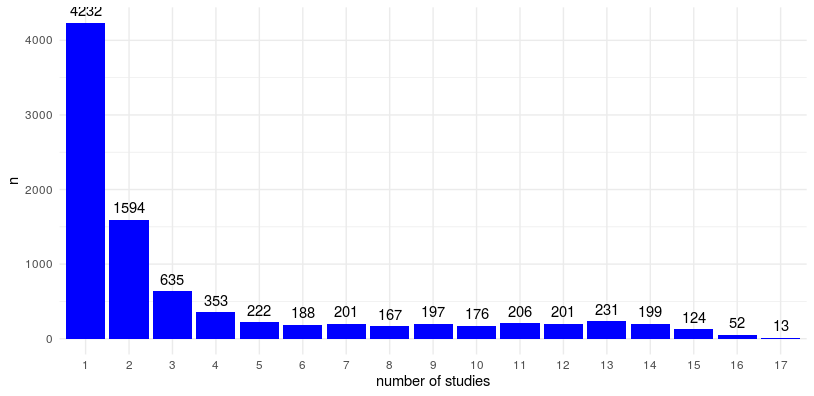
\includegraphics[width=\textwidth]{images/chapter3/ggplot2/essential_genes/Rplot_num_studies_in_DEG_corrected.png}
    \caption{Number of datasets genes in Database of Essential Genes appear in. Twenty nine genes appearing in forty two studies for which consistent entrez ID could not be established were removed. }
    \label{fig:num_studies_database_essential_genes}
\end{figure}
\subsection{Loss of function and evolutionary pressure ExAC and gnomad}
\label{sec:methods exac and gnomad}
The Exome Aggregation Consortiuim (ExAC) database collects the data from the exomes of over 60,000 individuals to providing a measure of the tolerance to mutation in genes and genetic loci\cite{lek2016analysis}. Comparing the number of loss of function mutations to the the number of harmless synonymous mutations provides a measure of how intolerant to mutation a gene or genetic region is in a population. The consortium provide a statistic, the probability of loss of function intolerance (pLI), that measures how much purifying selection a gene is under\footnote{The data was downloaded from \url{"https://storage.googleapis.com/gnomad-public/legacy/exac_browser/forweb_cleaned_exac_r03_march16_z_data_pLI_CNV-final.txt.gz"} (valid on 16.06)}, taking into account confounding factors such as gene size. 

To test the hypothesis that central genes are more likely to be essential and by extension intolerant of mutation I measured the correlation coefficient between pLI and centrality measures such as degree. Likewise to determine whether genes associated with intelligence and educational attainment were more likely to be loss of function intolerant I calculated the correlation between gene z score and the -log10 transform of the gene p value. 

 Very recently a greatly enlarged successor the Genome Aggregation Database (gnomAD) has become available and I have repeated the analysis using this. It aggregates 15,708 whole genomes and 125,748 exomes across 141,456 subjects. This increases the number of small genetic variations reported to 241 million compared with 7.4 million by ExAC and thus a more complete picture of genetic constraint can be obtained\cite{karczewski2020mutational}. Educational attainment (and schizophrenia) have been reported to be the most enriched traits with constraint\cite{karczewski2020mutational}\footnote{specifically decile of LOEUF `90\% upper bound of this confidence interval, which we term the loss-of-function observed/expected upper bound fraction (LOEUF) (Extended Data Fig. 7b, c),\cite{karczewski2020mutational}'} but the level of constraint in the PSP and the association between constraint and network features remain unreported.  

Gnomad v2.1.1 loss of function metrics by gene were downloaded from the consortium's cloud storage url\footnote{\url{https://storage.googleapis.com/gnomad-public/release/2.1.1/constraint/gnomad.v2.1.1.lof_metrics.by_gene.txt.bgz}}. This is the 6th of March 2019 release and contains loss of function summary metrics by gene\footnote{gnomad v3 is available but does not have these summary data}.

The file contained 19704 rows and 77 columns. Three gene identifiers are provided: Ensembl Gene ID, Ensembl transcript ID and HGNC Symbol with 19658 unique Gene Symbols and 19704 unique Ensembl IDs.

Translating Ensembl ID to Entrez ID do not always result in a one to one mapping. I tried Ensembl ID and Gene Symbol to determine which performed best and used both gprofiler2\footnote{\url{https://CRAN.R-project.org/package=gprofiler2 }} R interface (v0.2) to the g:Profiler toolset\cite{raudvere2019g} and the ToppGene API\footnote{See discussion I had by this stage largely stopped using flat files from EntrezGene and BioMart which I had used at the start because of the good performance of both gprofiler2 and the ToppGene API.}. The best result was obtained using Ensembl ID and gprofiler2 resulting in 18782 unique entries, 46 ambiguous/duplicated which were removed and 983 which could not be mapped to an Entrez Gene ID. 

The ToppGene translation API using a custom python script\footnote{\url{/home/grant/RProjects/db_essential_genes/python/toppgene_api.ipynb}} resulted in 18604 unambigous, unique Entrez ID terms and because of better performance and avoiding using R and Python in the analysis I used the R gprofiler2 package\footnote{Using script download gnomad \url{source('~/RProjects/db_essential_genes/R/gnomad/download_gnomad.R')}}.  Both translations are available in csv format in the supplementary material\footnote{Using Ensebml ID to translate resulted in 19881 rows and 1005 duplicated entrez id.Using Gene ID to translate resulted in 20040 1896 duplicated},\footnote{Using the ToppGene API you get 18604 terms \url{/home/grant/RProjects/db_essential_genes/python/toppgene_api.ipynb}}.

    In translating Ensembl ID 1185 Ensembl ID could not be translated to Entrez ID and were excluded. Forty eight duplicate Entrez ID were generated in the translation process and these too were excluded. The data cleaning is documented in an R markdown file\footnote{\url{~/RProjects/db_essential_genes/R/gnomad/mkd_download_gnomad.Rmd}. 18717 genes have an Entrez ID associated with a Gnomad record. Of these 338 have NaN pLI values and were excluded resulting in 18379 records. 3407 PSP gnomad records are found (98.6\% of PSP).
}.  % Using script download gnomad \url{source('~/RProjects/db_essential_genes/R/gnomad/download_gnomad.R')}. I used the probability of loss of function intolerance (pLI) to measure of selection pressure on a gene. pLI is a probability and has a range 0-1. A pLI of 1 corresponds to the gene being totally loss of function intolerant (high pLI - more conserved gene)

% See also section~\ref{sec: exac methods from chapter community detection}
% The original results using ExAC are in the supplementary material section~\ref{sec:Processing and cleaning Exac data for PSP}




% \footnote{g profiler using Ensembl ID
% 983 none
% 46 duplicated}.
% df\_out3 = 18782



% \subsection{Gnomad}

% \textcolor{red}{check this again}

% 19704 rows and 77 columns. (CHECK) Ensembl ID was translated to Entrez ID using gprofiler 2. 1185 Ensembl ID were not identified and excluded. 48 Duplicate entrez id were generated and excluded. 

% This resulted in 18551 genes with 3417 in the PSP (correct) with 4 missing values for pLI. (looks like it is 18782 and only 983 none).

% There are 3413 PSP genes with valid pLI and 15030 other genes. 

% 507 of the gnomad v2.1.1 pLI values were NA - 19197 valid pLI values

% 18443 valid pLI with translation to entrez (96.07\% of available data)

% 3413/3457 (98.7\%) of PSP data.


% \textcolor{red}{checking this again}

% \url{source('~/RProjects/db_essential_genes/R/gnomad/download_gnomad.R')}

% gnomad v2.1.1. lof metrics by gene file

% 19704 rows and 77 columns
% Gene ID column is ENSG
% Gene is HGNC symbol




% 19704 rows of downloaded document 77 columns

% after translation using gprofiler ENSG to entrez and removal of duplicated ids (ie ambigious and NaN) see
% markdown file \url{~/RProjects/db_essential_genes/R/gnomad/mkd_download_gnomad.Rmd}

% 18717 entrez ensg pairs
% inner join (dplyr) with no data loss (ie 18717 out) on ENSG

% translated table
saved as RDS and table txt

\textcolor{red}{here now}
% latex table generated in R 3.6.1 by xtable 1.8-4 package
% Sat Oct 17 16:31:15 2020




\section{Cohorts and samples}
\label{Centrality:cohorts and samples}
\todo{do correlation centrality with murine ltp group}
The population data used to assign significance values to the association of genes and intelligence and educational attainment and to test the association of theses genes with centrality measures are described in sections~\ref{sec:cohorts from paper section} and \ref{sec:samples from paper section}.

Gene level statistics were derived from MAGMA as outlined in section ref~\ref{sec:MAGMA gene level methods}.




%%%%%%%%%%%%%%%%%%%%%%%%%%%    RESULTS  %%%%%%%%%%%%%%%%%%%%%%%%%%%%%%%%%%%%%%%%%%%%%%%%%%%%%

%%%%%%%%%%%%%%%%%%%%%%%%%%%    RESULTS  %%%%%%%%%%%%%%%%%%%%%%%%%%%%%%%%%%%%%%%%%%%%%%%%%%%%%

%%%%%%%%%%%%%%%%%%%%%%%%%%%    RESULTS  %%%%%%%%%%%%%%%%%%%%%%%%%%%%%%%%%%%%%%%%%%%%%%%%%%%%%

%%%%%%%%%%%%%%%%%%%%%%%%%%%    RESULTS  %%%%%%%%%%%%%%%%%%%%%%%%%%%%%%%%%%%%%%%%%%%%%%%%%%%%%

%%%%%%%%%%%%%%%%%%%%%%%%%%%    RESULTS  %%%%%%%%%%%%%%%%%%%%%%%%%%%%%%%%%%%%%%%%%%%%%%%%%%%%%

%%%%%%%%%%%%%%%%%%%%%%%%%%%    RESULTS  %%%%%%%%%%%%%%%%%%%%%%%%%%%%%%%%%%%%%%%%%%%%%%%%%%%%%

%%%%%%%%%%%%%%%%%%%%%%%%%%%    RESULTS  %%%%%%%%%%%%%%%%%%%%%%%%%%%%%%%%%%%%%%%%%%%%%%%%%%%%%



\section{RESULTS}

\todo{? divide into graph level and vertex level}
\paragraph{Vertex level measures}
\section{Summary of centrality measures}
    A histogram showing the distribution of centrality measures is shown in figure~\ref{fig:multiplot centrality histograms}. The distributions of the centralities  can be seen in figure~\ref{fig:multiplot centrality histograms}. The plots of degree, eigenvector centrality and betweenness centrality in particular have a heavy right tail with the mean greater than the median. The mean degree for the PSP network, for example, was 17.6 and its median 8.Indeed all of the distributions appear far from a normal Gaussian distribution except for the  closeness centrality. The K core index has a relatively uniform distribution. There is a marked peak at 0 for transitivity consistent with the saturation of transitivity values at this level which has been extensively discussed already. 
    
Summary statistics for the centrality measures are shown in table \ref{Table:Summary of centrality measures1}. The local transitivity is reported first with isolates (nodes with degree $k=1$\footnote{there are no nodes with $k=0$}) set to zero ($C_i^0$ - transitivity0) and second  ($C_{i}^{NaN}$ - TransitivityNA) where nodes of degree one ($k=1$) have an undefined transitivity and are removed from caclulations of summary statistics or correlation\footnote{because for a node with degree=1 the denominator $\frac{k_v(k_v)-1}{2}$ in equation~\ref{eq:local_transitvity}  would be 0)}.  There were 304 nodes of degree one ($k=1$). 

% Below this is reported the alternate method also implemented in igraph (isolates="zero") of setting nodes with degree 1 to have a local transitivity of 0 ($C_i^0$). \textcolor{red}{no you are not just now} Where not explicitly stated in subsequent results I am using the default method (remove nodes with $k=0$ from the calculations).
\todo{add graph}
The eigenvector centrality has been scaled to have a maximum value of one and local transitivity (local clustering coefficient) lies in the range 0-1. The betweenness is shown as the number of shortest paths going through a node and scaled in the range 0-1.
    Closeness centrality \todo{add this} does not follow a power law distribution \cite{newman2018networks}\footnote{p331-332} as it has a limited distribution as the reciprocal of the shortest path length from a node to all other nodes.   
    
\subsubsection{High betweenness Low Degree}
following \cite{joy2005high} see \url{source('~/RProjects/chapter3/R/betweenness/betweenness_degree_sim.R')}
\subsection{kcoreness results}
 The minimum shell index is 1, all of the 1 kcore corresponds to the connected component. The range of shell index is 1-24. The median shell index of a vertex is 8 and the mean value 9.15 (although shell indexes take on integer values). The distribution of these values is shown in figure~\ref{fig:Kcore_histogram}\todo{nice ish image of kcore already in core periphery section}
 
 \begin{figure}
     \centering
     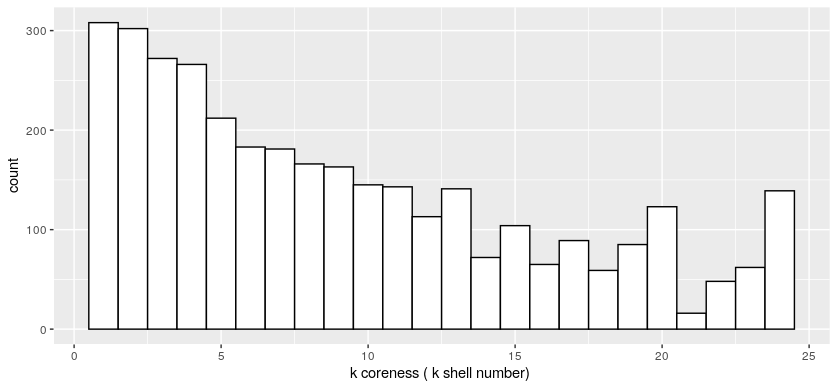
\includegraphics[width=\textwidth]{images/Rplot01_kcore_hist.png}
     \caption{Histogram of shell index of vertices in calculation of kcore. Shell index is the maximum kcore a vertex is a member of and not a member of shell index n+1. }
     \label{fig:Kcore_histogram}
 \end{figure}
 
 \textcolor{red}{to do U shaped ness of k core}\cite{burleson2020k} 
 
 See also \cite{dorogovtsev2006k}
\subsection{Testing the normality of centrality measures}
% latex table generated in R 3.6.3 by xtable 1.8-4 package
% Sat Jun 13 15:54:02 2020

Visual inspection of the histogram of the distribution of centrality measures in figure~\ref{fig:multiplot centrality histograms} suggest that the only one with a distribution that loos close to normal is the closeness cnetrality and degree, betweennness and eigenvector centrality are heavy tailed. 

% All of the centrality measures appear to vary from a normal distribution using the Shaprio-Wilk test in R and in accordance with their plots(table~\ref{tab:Test for normality (Shapiro-Wilk) for centrality measures of PSP}) . Spearman's test of correlation will therefore be used for correlation with centrality measures.



% \begin{figure}
%     \centering
%     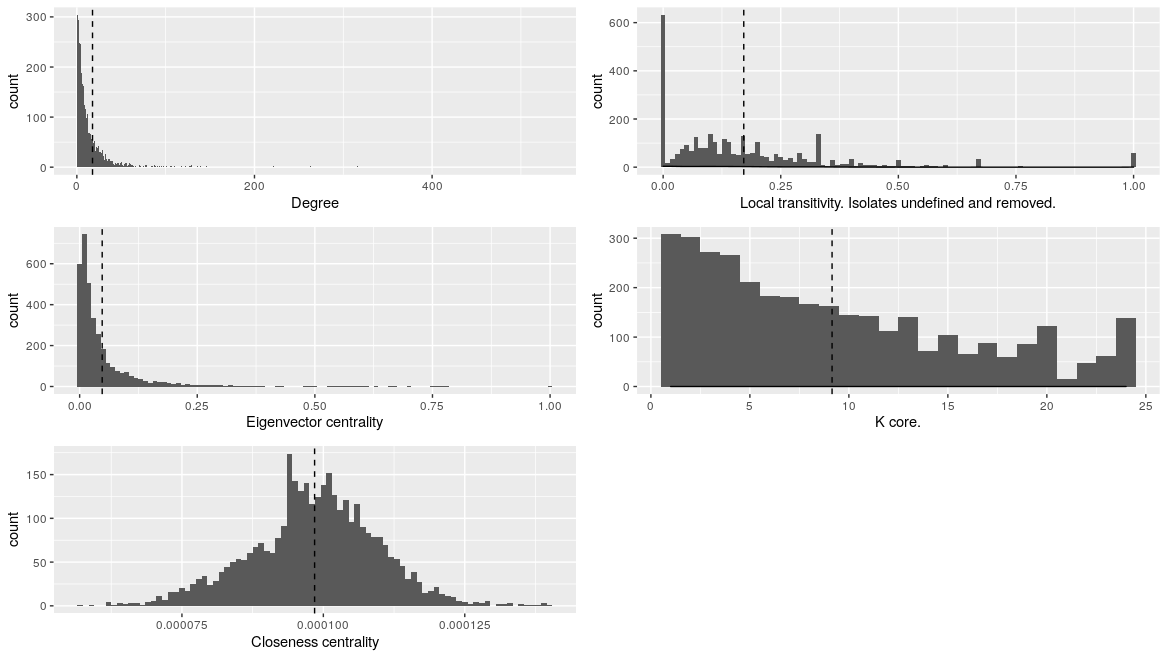
\includegraphics[width=\textwidth]{images/Rplot_histogram_centralities.png}
%     \caption{Multiplot of histogram of centrality measures. Dashed line is median}
%     \label{fig:multiplot centralities}
% \end{figure}
To confirm this and determine the most appropriate method of testing correlation of gene scores and measures of mutation intolerance with centrality scores a Shapiro-Wilk test was performed using R (see table~\ref{tab:Test for normality (Shapiro-Wilk) for centrality measures of PSP}). The results of the Kolmogorov Smirnov test calculating the statistic for the difference between the empirical distribution and the normal distribution with identical mean and standard deviation is shown in table~\ref{tab:Test for normality (KS) for centrality measures of PSP}.

These confirm that the centrality measures are not normally distributed, and a non parametric test of correlation (Spearman's rho) is appropriate \footnote{\url{source('~/RProjects/paper_xls_latex/R/centrality_summary/centrality_summary_latex.R')}} in accordance with practice in the more recent literature \cite{oldham2019consistency}\footnote{but not Valente\cite{valente2008correlated}}.


% latex table generated in R 3.6.2 by xtable 1.8-4 package
% Mon Feb 10 14:17:12 2020
% \begin{table}[ht]
% \centering
% \begin{tabular}{rrrrrrr}
%   \hline
%  & Minimum & 1st Quartile & Median & Mean & 3rd Quartile & Maximum \\ 
%   \hline
% Degree & $1 $ & $4 $ & $8 $ & $17.64$  & $19$ & $535$ \\ 
%   Eigenvector & $1.821 \times 10^{-6}$ & $8.829 \times 10^{-3}$ & $2.194 \times 10^{-2}$ & $4.793 \times 10^{-2}$ & $5.322 \times 10^{-2}$ & $1 $ \\ 
%   Betweenness & $0 $ & $43.29 $ & $317 $ & $3421.1$ & $1571.6$& $6.447 \times 10^{5}$ \\ 
%   Transitivity & $0 $ & $4.376 \times 10^{-2}$ & $1.290 \times 10^{-1}$ & $1.714 \times 10^{-1}$ & $2.381 \times 10^{-1}$ & $1 $ \\ 
%   Closeness & $5.702 \times 10^{-5}$ & $9.217 \times 10^{-5}$ & $9.879 \times 10^{-5}$ & $9.845 \times 10^{-5}$ & $1.058 \times 10^{-4}$ & $1.399 \times 10^{-4}$ \\ 
%   \hline
% \end{tabular}
% \caption{Summary of centrality measures} 
% \label{Table:Summary of centrality measures}
% \end{table}
% Table created by stargazer v.5.2.2 by Marek Hlavac, Harvard University. E-mail: hlavac at fas.harvard.edu
% Date and time: Tue, Nov 10, 2020 - 16:35:43





% latex table generated in R 3.6.3 by xtable 1.8-4 package
% Sun Mar  7 13:07:50 2021
\begin{table}[ht]
\centering
\begin{adjustbox}{width=\textwidth}

\begin{tabular}{rrrrrrrrr}
  \toprule
 & Degree & Betweenness & Bet 0-1 & Eigenvector & Closeness & Transitivity0 & TransitivityNA & kcoreness \\ 
  \midrule
Min. & 1.0 & 0.0 & $0.0$ & $1.82 \times 10^{-6}$ & $5.70 \times 10^{-5}$ & 0.00 & 0.00 & 1.0 \\ 
  1st Qu. & 4.0 & 43.3 & $7.25 \times 10^{-6}$ & $8.83 \times 10^{-3}$ & $9.22 \times 10^{-5}$ & 0.00 & 0.04 & 3.0 \\ 
  Median & 8.0 & 317.0 & $5.31 \times 10^{-5}$ & $2.19 \times 10^{-2}$ & $9.88 \times 10^{-5}$ & 0.11 & 0.13 & 8.0 \\ 
  Mean & 17.6 & 3421.1 & $5.73 \times 10^{-4}$ & $4.79 \times 10^{-2}$ & $9.85 \times 10^{-5}$ & 0.16 & 0.17 & 9.2 \\ 
  3rd Qu. & 19.0 & 1571.6 & $2.63 \times 10^{-4}$ & $5.32 \times 10^{-2}$ & $1.06 \times 10^{-4}$ & 0.22 & 0.24 & 13.0 \\ 
  Max. & 535.0 & 644670.7 & $1.08 \times 10^{-1}$ & $1.0 $ & $1.40 \times 10^{-4}$ & 1.00 & 1.00 & 24.0 \\ 
   \bottomrule
\end{tabular}
\end{adjustbox}
\caption[Summary centrality statistics]{Summary centrality Statistics for the PSP showing minimum value, 1st quartile, median, mean, 3rd quartile and maximum. Bet 0-1 is betweenness scaled by maximum possible betweenness\footnote{$\frac{(N-1)(N-2)}{2}$}. TransitivityNA has isolates set to NA. Number of NA: 304. The value of transitivityNA ($C_i^{NaN}$) is slightly greater than transitivity with isolates set to zero (Transitivity0 $C_i^0$)\textcolor{red}{add source}} 
\label{Table:Summary of centrality measures1}
\end{table}







\todo{density plot of tranitivityNA and transitivity0 showing probability around 0}
\begin{figure}
    \centering
    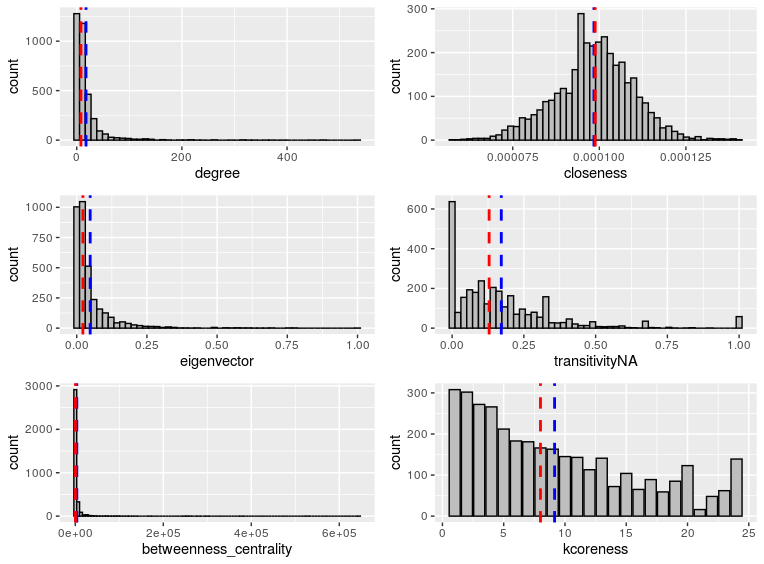
\includegraphics[width=\textwidth]{images/chapter3/ggplot2/Rplot_histogram+_centrality_multiplot.png}
    \caption[Multiplot histogram of centrality measures]{Multiplot histogram of centrality measures. Bin size kept constant at 50 other than barplot for kcoreness. Median is red dashed line, mean is blue dashed line. Plots are of (clockwise from top right: closeness centrality, local transitivity with isolates removed (transitivityNA), kcoreness, betweenness centrality, eigenvector centrality and degree centrality. Degree, eigenvector and betweenness centrality have particularly marked heavy tailed distributions suggestive of a power law. The closeness centrality looks similar to a normal distribution.   \url{source('~/RProjects/chapter3/R/essential_genes/histogram_centralities/multiplot_centralities.R')}}
    \label{fig:multiplot centrality histograms}
\end{figure}

\todo{Global transitivity and compare}
\todo{query pull out the global measures eg degree assortativity, transitivity}

% % Shapiro Wilk table
% \begin{table}[h]
%     \centering
%     \begin{tabular}{c|c|c}
%       Centrality measure  &  W & p\\
%       \hline
       
%       Degree  & 0.426 & $<2.2 \times 10^{-16}$ \\
%       Eigenvector &0.561  & $<2.2 \times 10^{-16}$ \\
%       Betweenness &0.1228& $<2.2 \times 10^{-16}$ \\
%       Transitivity &0.782 & $<2.2 \times 10^{-16}$\\
%       Closeness &0.9953& $<4.686 \times 10^{-09}$\\ 
%     \end{tabular}
%     \caption{Test for normality (Shapiro-Wilk) for centrality measures of PSP\textcolor{red}{add kcore}}
%     \label{tab:Test for normality (Shapiro-Wilk) for centrality measures of PSP}
% \end{table}

% latex table generated in R 3.6.3 by xtable 1.8-4 package
% Sun Feb 21 09:31:11 2021
\begin{table}[ht]
\centering
\begin{tabular}{rrr}
  \toprule
 & W & p value \\ 
  \midrule
Degree & 0.425 & $2.52 \times 10^{-74}$ \\ 
 Betweenness & 0.123 & $2.76 \times 10^{-83}$ \\ 
 Eigenvector & 0.561 & $6.55 \times 10^{-69}$ \\ 
 Closeness & 0.995 & $4.69 \times 10^{-9}$ \\ 
 Transitivity0 & 0.775 & $2.65 \times 10^{-56}$ \\ 
 Kcoreness & 0.911 & $4.32 \times 10^{-41}$ \\ 
   \bottomrule
\end{tabular}
\caption[Shapiro-Wilk tests for centrality measures in the PSP]{Test for normality (Shapiro-Wilk) for centrality measures of PSP.
\url{source('~/RProjects/chapter3/R/centrality_ch3/summary_centrality_sw.R')}}
\label{tab:Test for normality (Shapiro-Wilk) for centrality measures of PSP}
\end{table}

% latex table generated in R 3.6.3 by xtable 1.8-4 package
% Tue Nov 10 17:32:27 2020
\begin{table}[ht]
\centering
\begin{tabular}{rrr}
  \toprule
 & D & p value \\ 
  \midrule
Degree & 0.311 & $<2.2 \times 10^{-16}$ \\ 
  Betweenness & 0.434 & $<2.2 \times 10^{-16}$ \\ 
  Eigenvector & 0.269 & $<2.2 \times 10^{-16}$ \\ 
  Closeness & 0.046 & $7.174 \times 10^{-7}$ \\ 
  Transitivity0 & 0.198 & $<2.2 \times 10^{-16}$ \\ 
  kcoreness & 0.126 & $<2.2 \times 10^{-16}$ \\ 
   \bottomrule
\end{tabular}
\caption[Kolmogorov-Smirnov tests - centrality measures in the PSP]{JOIN THIS WITH SHAPIRO WILKTest for normality Kolmogorov-Smirnov centrality measures PSP. For local transitivity isolates are set to zero. \url{source('~/RProjects/chapter3/R/centrality_ch3/summary_centrality_ks.R')}}
\label{tab:Test for normality (KS) for centrality measures of PSP}
\end{table}
\section{Correlation of centrality measures}
\label{sec:correlation of centrality measures results section}
The pairwise relation between centrality measures is shown in the scatterplot in figure~\ref{tab:Correlation of centrality measures 2 transitvities} and SUPPLE\ref{fig:scatter plot of multiple centralities gg ally}. 






\subsection{Correlation of centrality measures}

All of the centrality measures appear significantly correlated except between transitivity and betweenness centrality (table~\ref{tab:Correlation of centrality measures 2 transitvities}). The transitivity has been viewed as an inverse betweenness (section~\ref{sec:local clustering coefficient}) and if so it is more marked with isolates set to NA when the distribution is not as dominated by zero values. Spearman's rank correlation with pairwise complete observations included was used to calculate the correlation of centrality measures. Transitivity is most weakly correlated with other measures\footnote{Code \url{source('~/RProjects/paper_xls_output/R/make_df_correlation_between_centrality_measures.R')}}.

The global positive correlation between transitivity and centrality measures is largely caused by nodes of transitivity 0 or 1 (see section~\ref{sec:results_global_clustering_coefficient}) particularly when isolates are treated as 0 )$C_{WS}0$ as the lowest degree nodes ($k=1$) have zero transitivity by definition\footnote{Newman's criticism of the Watts-Strogatz global clustering coefficient as being dominated by nodes of small value is also exacerbated by setting isolates to zero.}.





% latex table generated in R 3.6.3 by xtable 1.8-4 package
% Tue Oct 20 16:40:12 2020
\begin{table}[ht]
\centering
\setlength{\extrarowheight}{2pt}
\begin{adjustbox}{width=\textwidth}
\begin{tabular}{rrrrrrrr}
  \toprule
 & degree & betweenness & eigenvector & closeness & transitivityNA & transitivity0 & kcoreness \\ 
  \midrule
degree & 1.000 & 0.902 & 0.879 & 0.851 & 0.196 & 0.375 & 0.986 \\ 
  betweenness & 0.902 & 1.000 & 0.762 & 0.782 & -0.002 & 0.209 & 0.854 \\ 
  eigenvector & 0.879 & 0.762 & 1.000 & 0.969 & 0.330 & 0.462 & 0.906 \\ 
  closeness & 0.851 & 0.782 & 0.969 & 1.000 & 0.292 & 0.430 & 0.872 \\ 
  transitivityNA & 0.196 & -0.002 & 0.330 & 0.292 & 1.000 & 1.000 & 0.265 \\ 
  transitivity0 & 0.375 & 0.209 & 0.462 & 0.430 & 1.000 & 1.000 & 0.428 \\ 
  kcoreness & 0.986 & 0.854 & 0.906 & 0.872 & 0.265 & 0.428 & 1.000 \\ 
   \bottomrule
 
   
\end{tabular}
\end{adjustbox}
\caption[Correlation of centrality measures]{Correlation of centrality measures. Spearman's rho. Method for NA data (transitivity isolates) include only pairwise complete. TransitivityNA treats isolates as NA and removes from calculation. Transitivity0 uses the option to set isolates to 0. Note only with NA does transitivity appear like an inverse of the betweenness but we have not checked over 5.  All $p<2.2 \times 10^{-16}$ other than correlation between transitivity NA and betweenness = 0.901 using package Hmisc and checking with native r cor.test. } 
\tiny Code at \url{source('~/RProjects/db_essential_genes/R/get_corr/cor_centrality_measures.R')}
\tiny Code at same address in object t \url{source('~/RProjects/db_essential_genes/R/get_corr/cor_centrality_measures_performance.R')}
\label{tab:Correlation of centrality measures 2 transitvities}
\end{table}

% % latex table generated in R 3.6.1 by xtable 1.8-4 package
% % Sun Mar  7 16:10:40 2021
% \begin{table}[ht]
% \centering
% \begin{tabular}{rllr}
%   \hline
%  & Centrality 1 & Centrality 2 & Cor rho \\ 
%   \hline
% 1 & transitivity0 & transitivityNA & 1.000 \\ 
%   2 & kcoreness & degree & 0.986 \\ 
%   3 & closeness & eigenvector & 0.969 \\ 
%   4 & kcoreness & eigenvector & 0.906 \\ 
%   5 & betweenness & degree & 0.902 \\ 
%   6 & eigenvector & degree & 0.879 \\ 
%   7 & kcoreness & closeness & 0.872 \\ 
%   8 & kcoreness & betweenness & 0.854 \\ 
%   9 & closeness & degree & 0.851 \\ 
%   10 & closeness & betweenness & 0.782 \\ 
%   11 & eigenvector & betweenness & 0.762 \\ 
%   12 & transitivity0 & eigenvector & 0.462 \\ 
%   13 & transitivity0 & closeness & 0.430 \\ 
%   14 & kcoreness & transitivity0 & 0.428 \\ 
%   15 & transitivity0 & degree & 0.375 \\ 
%   16 & transitivityNA & eigenvector & 0.330 \\ 
%   17 & transitivityNA & closeness & 0.292 \\ 
%   18 & kcoreness & transitivityNA & 0.265 \\ 
%   19 & transitivity0 & betweenness & 0.209 \\ 
%   20 & transitivityNA & degree & 0.196 \\ 
%   21 & transitivityNA & betweenness & -0.002 \\ 
%   \hline
% \end{tabular}
% \caption{Correlation of centrality measures. Spearman. Ordered by correlation. Method for missing data include only pairwise complete. TransitivityNA treats isolates as NA and removes from calculation. Transitivity0 uses the option to set isolates to 0\url{source('~/RProjects/db_essential_genes/R/get_corr/cor_centrality_measures_ordered_cortable.R')}} 
% \end{table}



% % latex table generated in R 3.6.1 by xtable 1.8-4 package
% % Sun Mar  7 16:19:10 2021
% \begin{table}[ht]
% \centering
% \begin{tabular}{rrrrrrrr}
%   \hline
%  & degree & betweenness & eigenvector & closeness & transitivityNA & transitivity0 & kcoreness \\ 
%   \hline
% degree & 1.000 & 0.827 & 0.815 & 0.769 & -0.086 & -0.086 & 0.958 \\ 
%   betweenness & 0.827 & 1.000 & 0.598 & 0.650 & -0.315 & -0.315 & 0.707 \\ 
%   eigenvector & 0.815 & 0.598 & 1.000 & 0.938 & 0.174 & 0.174 & 0.881 \\ 
%   closeness & 0.769 & 0.650 & 0.938 & 1.000 & 0.120 & 0.120 & 0.821 \\ 
%   transitivityNA & -0.086 & -0.315 & 0.174 & 0.120 & 1.000 & 1.000 & 0.058 \\ 
%   transitivity0 & -0.086 & -0.315 & 0.174 & 0.120 & 1.000 & 1.000 & 0.058 \\ 
%   kcoreness & 0.958 & 0.707 & 0.881 & 0.821 & 0.058 & 0.058 & 1.000 \\ 
%   \hline
% \end{tabular}
% \caption{Correlation of centrality measures. For nodes with degree five or more Spearman. Method for missing data include only pairwise complete. TransitivityNA treats isolates as NA and removes from calculation. Transitivity0 uses the option to set isolates to 0} 
% \label{tab:Correlation of centrality measures 2 transitvities deg five or more}
% \end{table}






% % latex table generated in R 3.6.1 by xtable 1.8-4 package
% % Sun Mar  7 16:19:10 2021
% \begin{table}[ht]
% \centering
% \begin{tabular}{rllr}
%   \hline
%  & Centrality 1 & Centrality 2 & Cor rho \\ 
%   \hline
% 1 & transitivity0 & transitivityNA & 1.000 \\ 
%   2 & kcoreness & degree & 0.958 \\ 
%   3 & closeness & eigenvector & 0.938 \\ 
%   4 & kcoreness & eigenvector & 0.881 \\ 
%   5 & betweenness & degree & 0.827 \\ 
%   6 & kcoreness & closeness & 0.821 \\ 
%   7 & eigenvector & degree & 0.815 \\ 
%   8 & closeness & degree & 0.769 \\ 
%   9 & kcoreness & betweenness & 0.707 \\ 
%   10 & closeness & betweenness & 0.650 \\ 
%   11 & eigenvector & betweenness & 0.598 \\ 
%   12 & transitivityNA & eigenvector & 0.174 \\ 
%   13 & transitivity0 & eigenvector & 0.174 \\ 
%   14 & transitivityNA & closeness & 0.120 \\ 
%   15 & transitivity0 & closeness & 0.120 \\ 
%   16 & kcoreness & transitivityNA & 0.058 \\ 
%   17 & kcoreness & transitivity0 & 0.058 \\ 
%   18 & transitivityNA & degree & -0.086 \\ 
%   19 & transitivity0 & degree & -0.086 \\ 
%   20 & transitivityNA & betweenness & -0.315 \\ 
%   21 & transitivity0 & betweenness & -0.315 \\ 
%   \hline
% \end{tabular}
% \caption{Correlation of centrality measures. Spearman. Degree five or more. Ordered by correlation. Method for missing data include only pairwise complete. TransitivityNA treats isolates as NA and removes from calculation. Transitivity0 uses the option to set isolates to 0. With degree 5 and over the negative correlation between degree and transitivity is cllearly seen and the role of the betweenness as a form of inverse the role of the betweenness as a form of inverse transitivity\url{source('~/RProjects/db_essential_genes/R/get_corr/cor_centrality_measures_ordered_cortable.R')}} 
% \end{table}



% latex table generated in R 3.6.1 by xtable 1.8-4 package
% Sun Mar  7 16:39:36 2021
% \begin{table}[ht]
% \centering
% \begin{tabular}{rllrrr}
%   \hline
%  & Centrality 1 & Centrality 2 & Cor rho & Cor rho deg gt 5 & Rank 5 \\ 
%   \hline
% 1 & transitivity0 & transitivityNA & 1.000 & 1.000 & 1 \\ 
%   2 & kcoreness & degree & 0.986 & 0.958 & 2 \\ 
%   3 & closeness & eigenvector & 0.969 & 0.938 & 3 \\ 
%   4 & kcoreness & eigenvector & 0.906 & 0.881 & 4 \\ 
%   5 & betweenness & degree & 0.902 & 0.827 & 5 \\ 
%   6 & kcoreness & closeness & 0.872 & 0.821 & 6 \\ 
%   7 & eigenvector & degree & 0.879 & 0.815 & 7 \\ 
%   8 & closeness & degree & 0.851 & 0.769 & 8 \\ 
%   9 & kcoreness & betweenness & 0.854 & 0.707 & 9 \\ 
%   10 & closeness & betweenness & 0.782 & 0.650 & 10 \\ 
%   11 & eigenvector & betweenness & 0.762 & 0.598 & 11 \\ 
%   12 & transitivity0 & eigenvector & 0.462 & 0.174 & 13 \\ 
%   13 & transitivityNA & eigenvector & 0.330 & 0.174 & 12 \\ 
%   14 & transitivity0 & closeness & 0.430 & 0.120 & 15 \\ 
%   15 & transitivityNA & closeness & 0.292 & 0.120 & 14 \\ 
%   16 & kcoreness & transitivity0 & 0.428 & 0.058 & 17 \\ 
%   17 & kcoreness & transitivityNA & 0.265 & 0.058 & 16 \\ 
%   18 & transitivity0 & degree & 0.375 & -0.086 & 19 \\ 
%   19 & transitivityNA & degree & 0.196 & -0.086 & 18 \\ 
%   20 & transitivity0 & betweenness & 0.209 & -0.315 & 21 \\ 
%   21 & transitivityNA & betweenness & -0.002 & -0.315 & 20 \\ 
%   \hline
% \end{tabular}
% \caption{} 
% \end{table}

% latex table generated in R 3.6.1 by xtable 1.8-4 package
% Sun Mar  7 16:48:58 2021



\begin{figure}
    \centering
    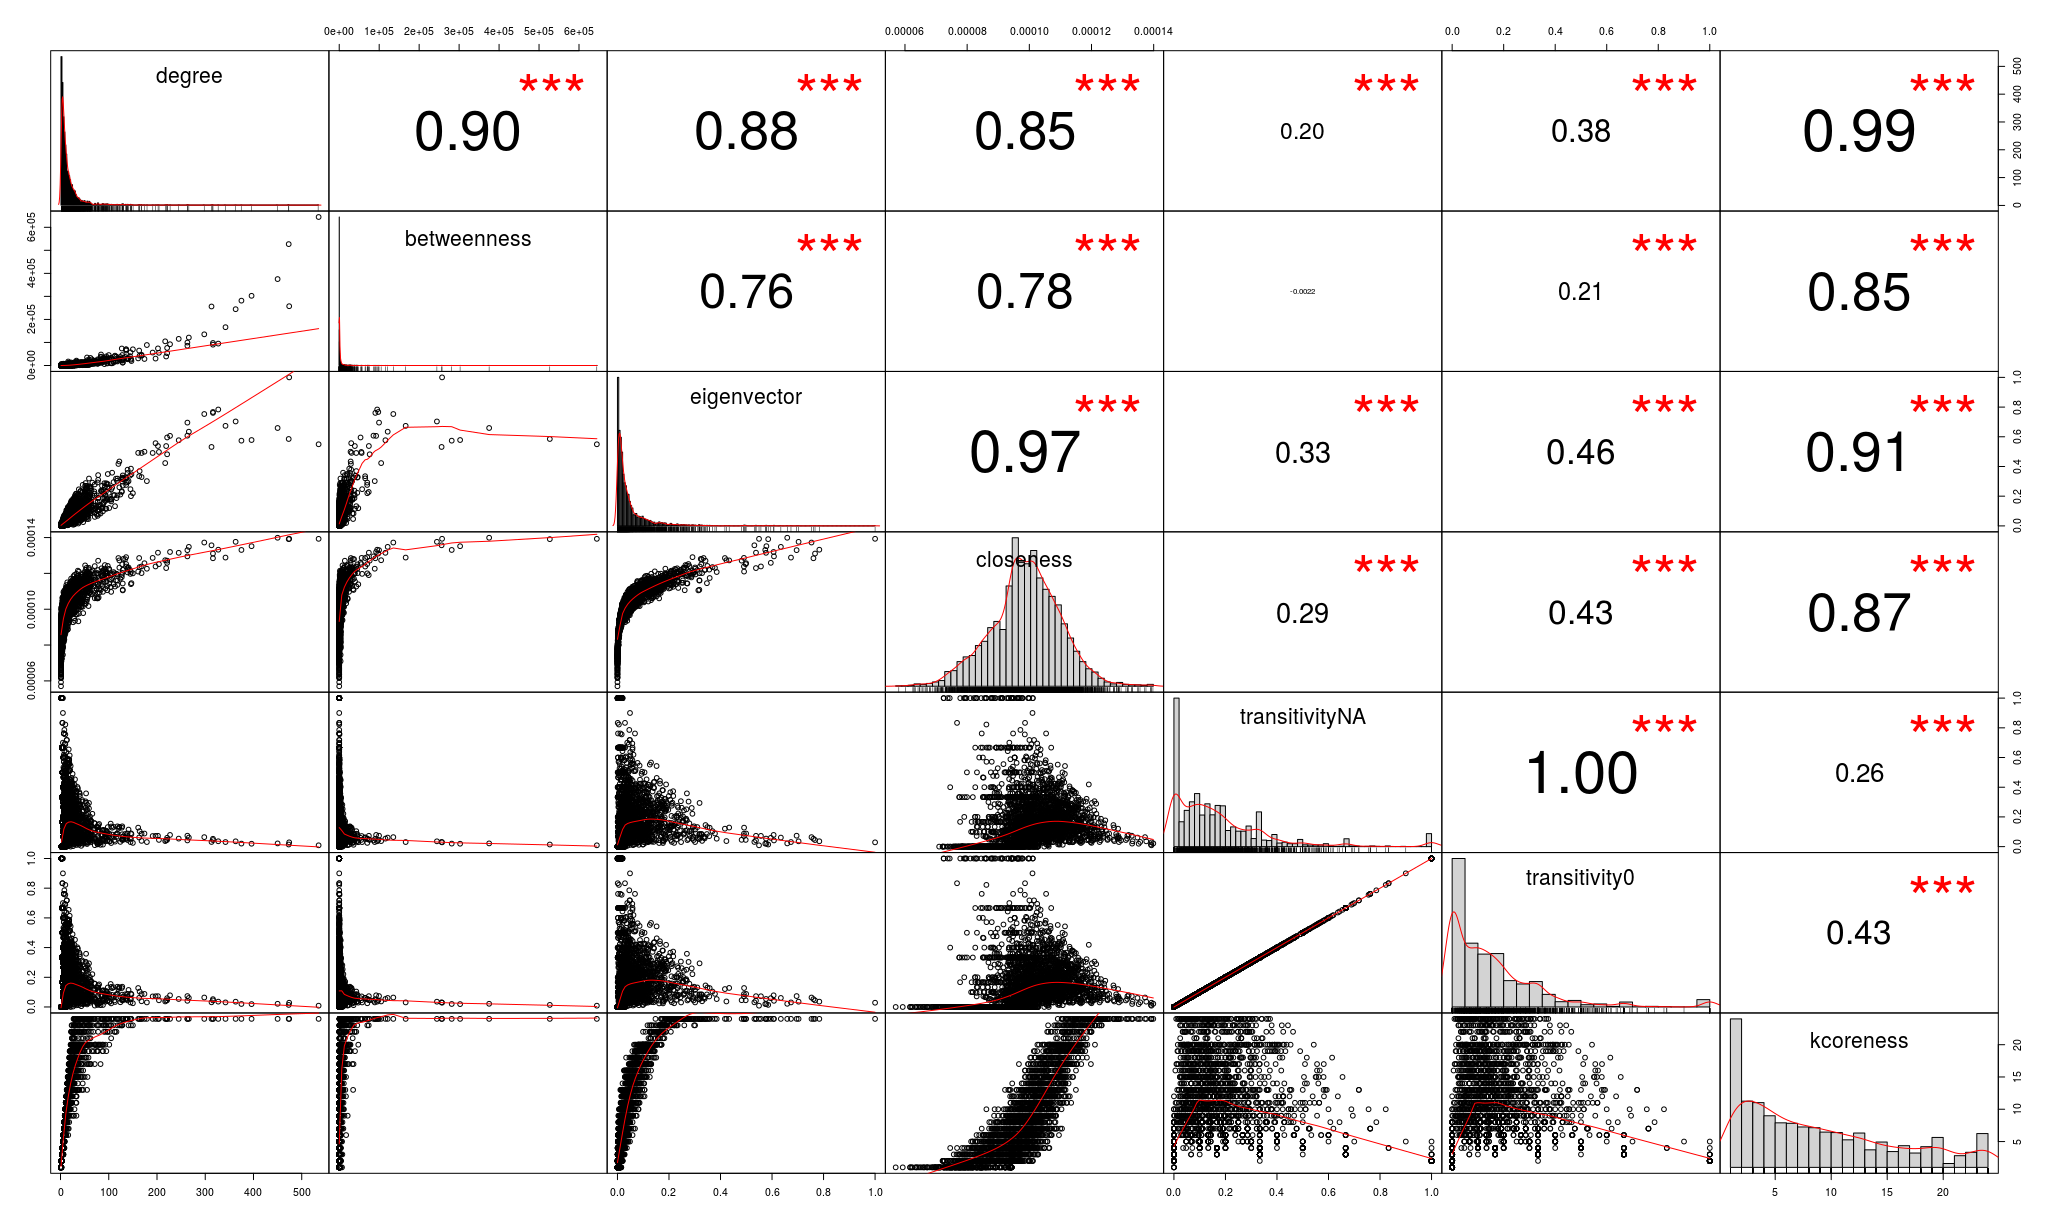
\includegraphics[width=\textwidth]{images/chapter3/cor_pairs/analytics/Rplot_analytics_spearman_cor.png}
    \caption{Correlation plot of centrality measures using package Performance Analytics. Deg = degree, eig= eigenvector centrality, clo = closeness centrality, bet = betweenness centrality, tra = local transitivity, kcore = kcoreness. Code at \url{source('~/RProjects/db_essential_genes/R/get_corr/cor_centrality_measures_performance.R')}}
    \label{fig:Correlation plot centrality performance analytics}
\end{figure}





% (I feel there is a stronger argument when there are a large number of degree zero nodes in the network and the largest component is smaller - ? move to discussion)\textcolor{green}{all of that was about transitivity}. 


  This is at variance with the view of local transitivity as a local betweenness where a node is central if transitivity is \textit{low} (see section~\ref{sec:local clustering coefficient}) and can be seen clearly if we test correlation for nodes of degree five or greater (tables SUPPLE~\ref{tab:Correlation of centrality measures 2 transitvities deg five or more} and \ref{tab:correlation and rank centrality five or more}).



\begin{table}[ht]
\centering
\begin{tabular}{llllll}
  \hline
Rank  & Centrality 1 & Centrality 2 &$\rho$ & $\rho_{k>=5}$  & Rank $k>=5$ \\ 
  \hline
1 & transitivity0 & transitivityNA & 1.00 & 1.00 & 1 \\ 
  2 & kcoreness & degree & 0.99 & 0.96 & 2 \\ 
  3 & closeness & eigenvector & 0.97 & 0.94 & 3 \\ 
  4 & kcoreness & eigenvector & 0.91 & 0.88 & 4 \\ 
  5 & betweenness & degree & 0.90 & 0.83 & 5 \\ 
  6 & kcoreness & closeness & 0.87 & 0.82 & 6 \\ 
  7 & eigenvector & degree & 0.88 & 0.81 & 7 \\ 
  8 & closeness & degree & 0.85 & 0.77 & 8 \\ 
  9 & kcoreness & betweenness & 0.85 & 0.71 & 9 \\ 
  10 & closeness & betweenness & 0.78 & 0.65 & 10 \\ 
  11 & eigenvector & betweenness & 0.76 & 0.60 & 11 \\ 
  12 & transitivity0 & eigenvector & 0.46 & 0.17 & 13 \\ 
  13 & transitivityNA & eigenvector & 0.33 & 0.17 & 12 \\ 
  14 & transitivity0 & closeness & 0.43 & 0.12 & 15 \\ 
  15 & transitivityNA & closeness & 0.29 & 0.12 & 14 \\ 
  16 & kcoreness & transitivity0 & 0.43 & 0.06 & 17 \\ 
  17 & kcoreness & transitivityNA & 0.26 & 0.06 & 16 \\ 
  18 & transitivity0 & degree & 0.38 & -0.09 & 19 \\ 
  19 & transitivityNA & degree & 0.20 & -0.09 & 18 \\ 
  20 & transitivity0 & betweenness & 0.21 & -0.31 & 21 \\ 
  21 & transitivityNA & betweenness & -0.00 & -0.31 & 20 \\ 
   \hline
\end{tabular}
\caption[Comparison of correlation coefficients for all nodes and nodes with degree greater than or equal to five]{Correlation of centrality measures. Spearman. Degree five or more. Ordered by correlation. Method for missing data include only pairwise complete. TransitivityNA treats isolates as NA and removes from calculation. Transitivity0 uses the option to set isolates to 0. There is minimal perturbation of the rank order but the relationship between transitivity and betweenness and degree become negative.}
\tiny\url{source('~/RProjects/db_essential_genes/R/get_corr/cor_centrality_measures_ordered_cortable_single_long_table.R')}
\label{tab:correlation and rank centrality five or more}
\end{table}

In addition it further obscures the relationship between transitivity and degree ( $C(k)$ and $k$ - section~\ref{sec:relationship of ck to k albert}) reported in biological networks, where high degree nodes have lower local clustering\todo{this is the second time for saying this now}\cite{albert2005scale}. Using $C_i^{NaN}$ has little effect on the correlation with other centrality measures or with gene statistics (table~\ref{tab:Correlation of centrality measures 2 transitvities}. When transitivity is of particular importance (such as calculating the small world phenomenon) I report both.


The most correlated centrality measures were degree and kcore (0.986). Excluding transitivity and kcoreness which are not amongst the canonical centrality measures \cite{okamoto2008ranking}\footnote{Four measures of centrality that are widely used in net-work analysis aredegree centrality,betweenness centrality4,closeness centrality,andeigenvector centrality5} the most correlated were eigenvector and closeness (0.969). This is higher than that reported in a collection of social science networks (0.63 in Valente et al\cite{valente2008correlated} - see table~\ref{tab:Correlation of centrality valente et al} and \ref{tab:Correlation of centrality valente et al compared with PSP}) 

See Oldham\cite{oldham2019consistency} for recent work on correlation across networks. Table~\ref{tab:Correlation of centrality valente et al} shows the results of the correlation between degree, eigenvector centrality, closeness and betweenness found by Valente et al.\cite{valente2008correlated} for 58 sociometric network datasets. Centrality measures appear more correlated in the PSP than in those reported by Valente particularly closeness and betweenness (0.44 vs 0.782) and degree and closeness (0.66 vs 0.85) see table~\ref{tab:Correlation of centrality valente et al compared with PSP} and persists even if lower degree nodes are removed from the calculation~\ref{tab:correlation and rank centrality five or more}) although Valente\cite{valente2008correlated} uses Pearson's product moment correlation.

Whether the higher correlation of closeness and other centrality measures may be a feature found in biological networks compared with social networks (as for example assortativity) is unclear\footnote{speculation ? to discussion}. 

\begin{table}[]
    \centering
    \begin{tabular}{lllll}
    \toprule
          & Degree & Eigenvector centrality & Closeness & Betweenness \\
         \midrule
    Degree  & 1  & 0.92  & 0.66 & 0.85\\
    Eigenvector centrality & 0.92 & 1 & 0.63 & 0.72  \\
    Closeness & 0.66 & 0.63 & 1 & 0.44  \\
    Betweenness& 0.85 & 0.72 & 0.44 & 1 \\
    \bottomrule
    \end{tabular}
    \caption[Correlation of centrality measures for sociometric networks]{Correlation of centrality measures for 58 sociometric network datasets from Valente et al \cite{valente2008correlated}. Pearson correlation coefficient. Values are for symmetrised closeness and betweenness centrality. Eigenvector centrality is necessarily symmetrised. Range of average network size 45-83. Some studies had maximal nominations for degree (i.e there was an artificial upper bound using a survey). Copied from notes.tex}
    \label{tab:Correlation of centrality valente et al}
\end{table}

\begin{table}[]
    \centering
    \begin{tabular}{lllll}
    \toprule
          & Degree & Eigenvector centrality & Closeness & Betweenness \\
         \midrule
    Degree  & 1  & 0.92 (0.88)  & 0.66 (0.851)*  & 0.85 (0.902)*\\
    Eigenvector centrality & 0.92 (0.88)  & 1 & 0.63 (0.969)* & 0.72 (0.762)  \\
    Closeness & 0.66 (0.851)  & 0.63 (0.969) & 1 & 0.44 (0.782)* \\
    Betweenness& 0.8 (0.902) & 0.72 (0.762) & 0.44 (0.782) & 1 \\
    \bottomrule
    \end{tabular}
    \caption[Correlation of sociometric centrality measures compared with correlation of measures in PSP]{Correlation of centrality measures for 58 sociometric network datasets from Valente et al.\cite{valente2008correlated}. Pearson correlation coefficient. Values are for symmetrised closeness and betweenness centrality. Eigenvector centrality is necessarily symmetrised. Range of average network size 45-83. Some studies had maximal nominations for degree (i.e there was an artificial upper bound using a survey). Copied from notes.tex. Comparison added with PSP * shows where PSP notably higher correlation.}
    \label{tab:Correlation of centrality valente et al compared with PSP}
\end{table}

\subsubsection{Principal component analysis of centrality measures}

Principal component analysis was carried out in order to allow dimensionality reduction in constructing a linear model of the effect of centrality measures and their interactions on educational attainment and intelligence genetic scores and to understand how the centrality measures are related to one another. 

Principal component analysis of centrality variables was carried out using the R command \texttt{prcomps}\footnote{which uses SVD} with the option \texttt{scale.=TRUE} for scaling the centralities to unit variance and all other arguments default. All centrality measures (six) other than transitivity NA were included (this was removed to avoid NA handling). The majority of the variance is explained by the first three principal components (93.4\%) (figure~\ref{fig:PCA_scree} and table~\ref{tab:Eigenvalue of dimensions of PCA for centrality measures with variance}).



\begin{figure}
    \centering
    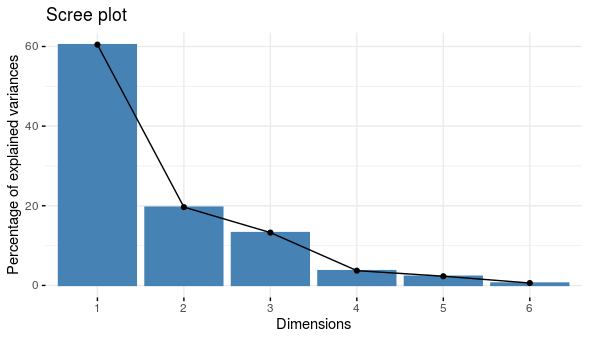
\includegraphics[width=\textwidth]{images/chapter3/centrality_pca_factoextra/Rplot_screeplot.png}
    \caption{Screeplot of the dimensions of centrality. TransitivityNA has been omitted to avoid dealing with NA. \url{source('~/RProjects/chapter3/R/centrality_ch3/prcomps/3_plotPCA.R')}}
    \label{fig:PCA_scree}
\end{figure}

% latex table generated in R 3.6.3 by xtable 1.8-4 package
% Sat Feb 20 17:09:15 2021
\begin{table}[ht]
\centering
\begin{tabular}{rrrr}
  \hline
Dimension & Eigenvalue & Variance (\%) & Cumulative variance (\%) \\ 
  \hline
Dim.1 & 3.63 & 60.46 & 60.46 \\ 
  Dim.2 & 1.18 & 19.66 & 80.12 \\ 
  Dim.3 & 0.80 & 13.26 & 93.38 \\ 
  Dim.4 & 0.22 & 3.71 & 97.09 \\ 
  Dim.5 & 0.14 & 2.31 & 99.40 \\ 
  Dim.6 & 0.04 & 0.60 & 100.00 \\ 
   \hline
\end{tabular}
\caption[Variance explained by PCA components of centrality measures]{Eigenvalue of dimensions of PCA for centrality measures with variance. Source \url{source('~/RProjects/chapter3/R/centrality_ch3/prcomps/5_PCA_eigval.R')}} 
\label{tab:Eigenvalue of dimensions of PCA for centrality measures with variance}
\end{table}
Transitivity and eigenvector centrality appear almost orthogonal in a plot of the first two dimensions (figure~\ref{fig:PCA_contributions}).



\begin{figure}
    \centering
    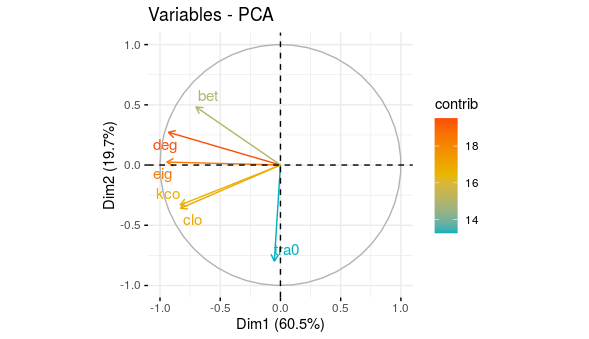
\includegraphics[width=\textwidth]{images/chapter3/centrality_pca_factoextra/Rplot_smaller_pca.png}
    \caption{Contribution of different variables. deg = degree, eig = eigenvector centrality, kco = kcore index, tra0 = transitivity with isolates set to zero, clo = closeness, bet = betweenness centrality.  \url{source('~/RProjects/chapter3/R/centrality_ch3/prcomps/3_plotPCA.R')}}
    \label{fig:PCA_contributions}
\end{figure}

A linear model of interactions of the first three principal components showed no significant variables impacting upon the  z-score of Education Discovery or Intelligence discovery \url{source('~/RProjects/chapter3/R/centrality_ch3/prcomps/6_cortest_lm.R')}

\clearpage
\section{Global network measures}




\subsection{Results Degree distribution}
\label{sec:results degree distribution}
The degree distribution of the PSP is right-skewed. The mean degree is greater than the median (17.6 vs 8), and the maximum degree (535) is over thirty times greater than the average degree. 
 The degree distribution $P(K=k)$ against degree $k$ is shown in figure~\ref{fig:Degree distribution of post synaptic proteome. Log10 - log10 scale1} on a doubly logarithmic scale, follows a relatively straight line in the tail of the distribution and would usually be considered to be consistent with a power law\footnote{or other distributions} in the tail of the distribution.

\begin{figure}
    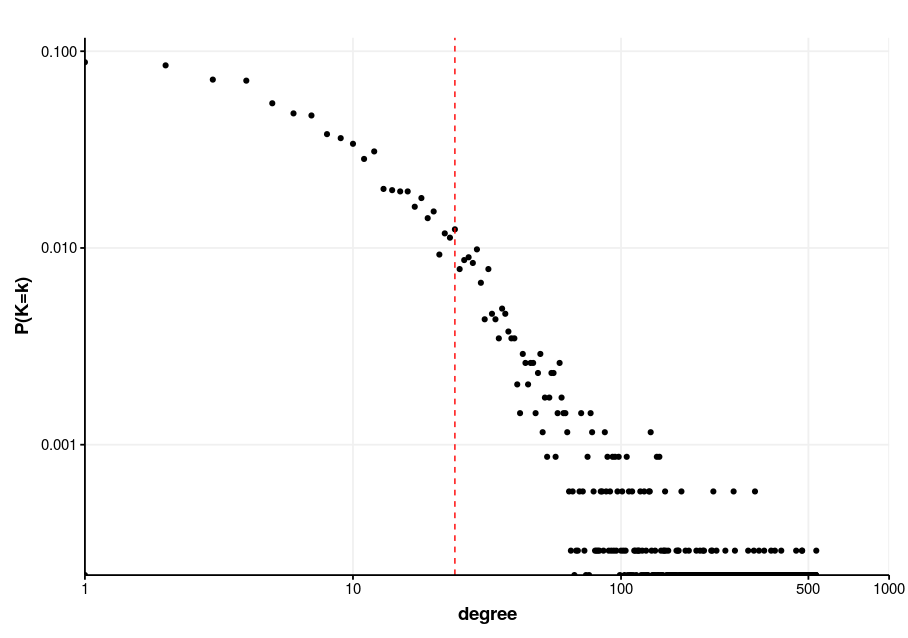
\includegraphics[width=12cm]{images/chapter3/poweRlaw/Rplot_degree_distribution_log10pktheme.png}
    \caption{Degree distribution of post synaptic proteome. Log10 - log10 scale.}
    \tiny Code at \url{source('~/RProjects/chapter3/R/fit_power_law/graphing/plot_degree_distribution_log10_theme_red_dotted_xmin.R')}\url{source('~/RProjects/gridsearch_gamma/R/plot_log_degreedist.R') }
    \label{fig:Degree distribution of post synaptic proteome. Log10 - log10 scale1}
\end{figure}


Using the method described by Clauset, Shalizi and Newman \cite{clauset2009power} to determine the presence of a power law distribution and implemented in the poweRlaw R package version 0.70.6 \cite{gillespie2015fitting} (section~\ref{sec: Methods degree distribution}) the minimum degree value ($x_{min}$) for which the power law distribution holds is first determined using the Kolmogorov-Smirnov (KS) statistic as a measure of goodness of fit (GOF) (section~\ref{sec: Methods degree distribution}). The value of $x_{min}$ is 24 and the power law coefficient $\gamma$ is 2.51 (table~\ref{tab:Fit of distributions for PSP})\footnote{, GOF 0.19 and  $n$tail (the number of nodes in the tail of the power law distribution i.e. greater than or equal to $x_{min}$) is 68 so there are a number of low degree  nodes outside the power law portion of the degree distribution\footnote{\url{source('~/RProjects/group_size_distribution/R/calulate_cdf.R')}}}. A bivariate plot of $x_{min}$ and $\gamma$ figure~\ref{fig:Plots of degree distribution}) shows that the power law exponent increases as the value of $x_{min}$ increases (also as main plot in figure~\ref{fig:gamma_main}).

The plot of log-degree against the log of the cumulative distribution function (CDF) of the degree distribution is shown in figure \ref{fig:log_degree_distribution} and  \ref{fig:poweRlaw plot ggplot2}. The graph forms a straight line for most of the distribution with degree greater than $x_{min}$\todo{?change plot or add vline for xmin}\footnote{the gradient of the CDF is $\gamma$-1}. In figure~\label{fig:poweRlaw plot ggplot2} the fit of the power law distribution is shown in red. 

The lines of fit of a power law, lognormal, exponential and Poisson distribution to the data are shown figure~\ref{fig:poweRlaw plot ggplot2} over the whole distribution (i.e. $x_{min}$ is calculated for each distribution as being the value for the fit that minimises the KS distance rather than $x_{min}$ equal to the power-law $x_{min}$ when comparing the log-likelihood of the distribution). This shows that in this case the lognormal can be a good model of the whole distribution.

In addition to determining that the distribution has an area in the tail that appears straight on a doubly logarithmic plot an estimate of the plausibility of a power law distribution was made by calculating the bootstrap $p$ value (100 sims) for the power law distribution is 0.583 with goodness of fit KS 0.19 \footnote{\url{source('~/RProjects/group_size_distribution/R/calulate_cdf.R')}}. A bootstrap $p$ value greater than 0.1 indicates that a power law distribution cannot be ruled out (see \cite{gillespie2015fitting} and \cite{clauset2009power}).



To determine the best fitting distribution, I calculated the log-likelihood of the power law, lognormal, exponential and Poisson distribution fitted to the data. The log-likelihoods were calculated for each distribution for the fit starting at $x_{min}$ determined for the power-law distribution $x_{min} = 24$ (see\cite{clauset2009power}) to allow direct comparison. The values of the parameters are in table~\ref{tab:Fit of distributions for PSP} along with the bootstrap $p$ value for each distribution. The plot of the distributions using $x_{min}=24$ is shown in figure~\ref{fig:models_set_xmin}.


\paragraph{Fit over xmin}
In assessing the portion for which a power law distribution holds ($x_{min}>24$) the log-likelihood is substantially lower than the exponential, log-normal\footnote{\url{https://www.sciencedirect.com/topics/agricultural-and-biological-sciences/lognormal-distribution}} or power law. 

\begin{figure}
    \centering
    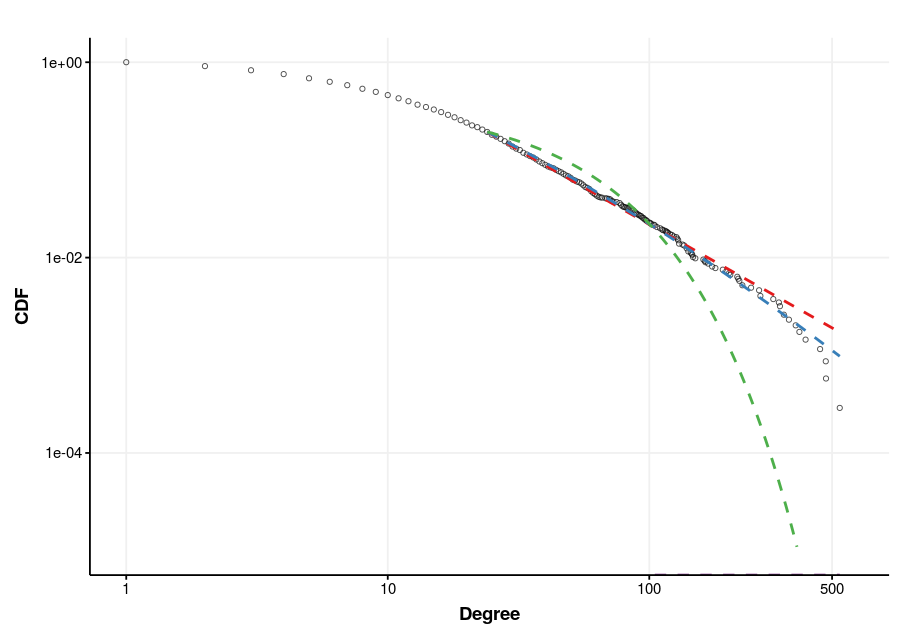
\includegraphics[width=\textwidth]{images/chapter3/poweRlaw/Rplot_models_xmin.png}
    \caption{CDF of degree distribution and lines of best fit for power law (red), log-normal(blue) exponential(green) and poisson (purple). Poisson distribution is not visible as the probability is too low, the exponential is a poorer fit in the tail of the distribution than either the powerlaw or log-normal . x axis degree log 10 scaled, y axis CDF log 10 scaled. Exponential appears a good fit but is fitted to a much smaller part of the distribution than the power law and log-normal. Poisson distribution is clearly not a good fit.}
    \small\url{source('~/RProjects/chapter3/R/fit_power_law/compare_distributions.R')}
    \label{fig:models_set_xmin}
\end{figure}

The exponential distribution is clearly inferior to log-normal and power law using goodness of fit bootstrap p or the two sided Vuong test (p=$3.455\times10^{-7}$). the power law versus exponential. The one sided Vuong test p = $1.72\times10^{-7}$ shows that the power law distribution is a better fit than the exponential as is clear in figure~\ref{fig:models_set_xmin}. 

There is no significant difference between the power law and log-normal using Vuong's two sided test (p=0.187). The one sided test favours the comparison of log-normal to power law (p=0.093)\footnote{power law v log-normal One sided p=0.906}.  

The level of confidence of a power law distribution according to the nested criteria of Broido and Clauset\cite{broido2019scale} for the PSP network is strong. The network is plausible by bootstrap $p$ (therefore stronger than weakest), $n_{tail}$ is greater than 50 (668 (at least weak) and meets the strong criteria by satisfying the previous ones and the exponent being between two and three (2.51). 10\% of the networks examined by Broido and Clauset had this characteristic. It does not meet strongest as the likelihood ratio test is inconclusive and does not favour either the log-normal or power law ($<$ 4\% of studied networks)




The distribution could be characterised either as a power law distribution or as a log-normal distribution.






\begin{figure}
    \centering
    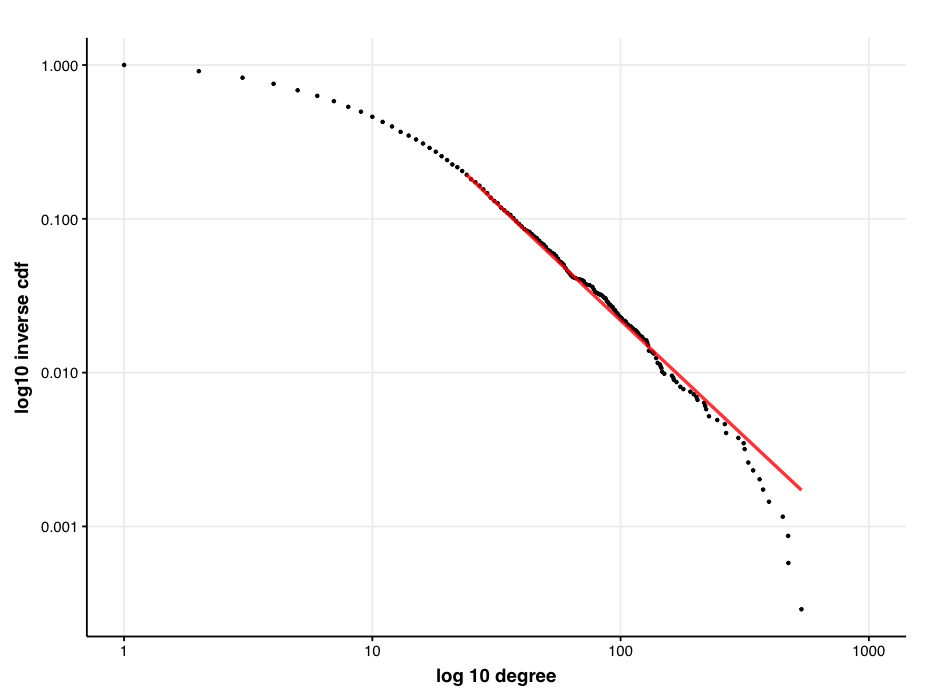
\includegraphics[width=\linewidth]{images/chapter3/ggplot2/theme/powerlaw/Rplot01_chapter3_cdf_and_powerlaw.png}
    \caption[Plot of power law fit to degree distribution of PSP]{Plot of fit of power law to degree distribution for the PSP. X axis is log 10 degree, Y axis is log 10 inverse cdf. Red line fit of power law distribution $\gamma= 2.51$ and $x_{min}=24$ \url{source('~/RProjects/group_size_distribution/R/calulate_cdf.R')}}
    \label{fig:poweRlaw plot ggplot2}
\end{figure}



\begin{figure}
    \centering
    \begin{subfigure}[t]{0.45\textwidth}
        \centering
        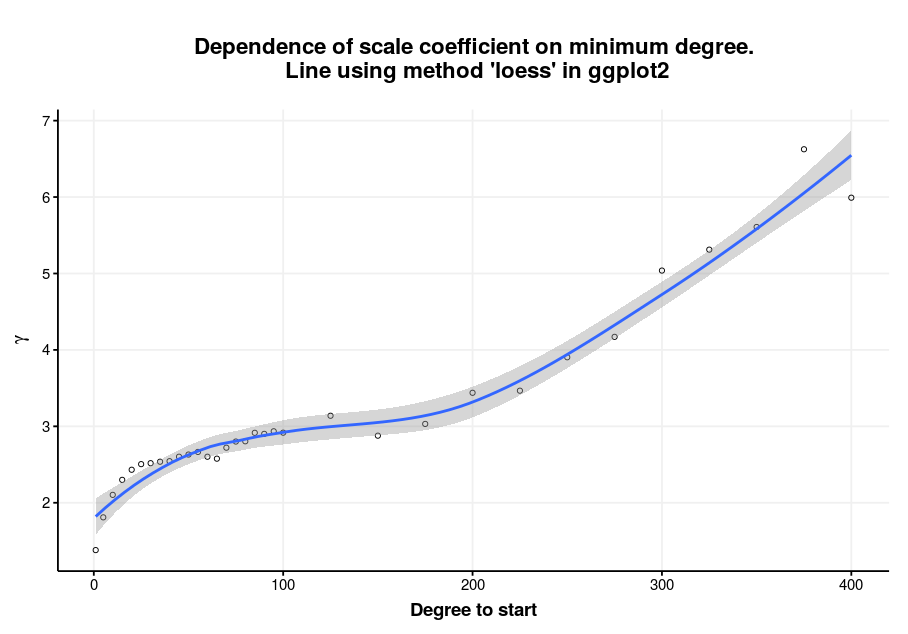
\includegraphics[width=\linewidth]{images/chapter3/poweRlaw/Rplot_gamma_theme.png} 
     \caption[$\gamma$ as function of $x_{min}$]{$\gamma$ as a function of $x_{min}$. }
    \tiny\url{source('~/RProjects/PhD_graphs/calculate_gamma_theme.R')}
        \label{fig:gamma}
    \end{subfigure}
    \hfill
    \begin{subfigure}[t]{0.45\textwidth}
        \centering
        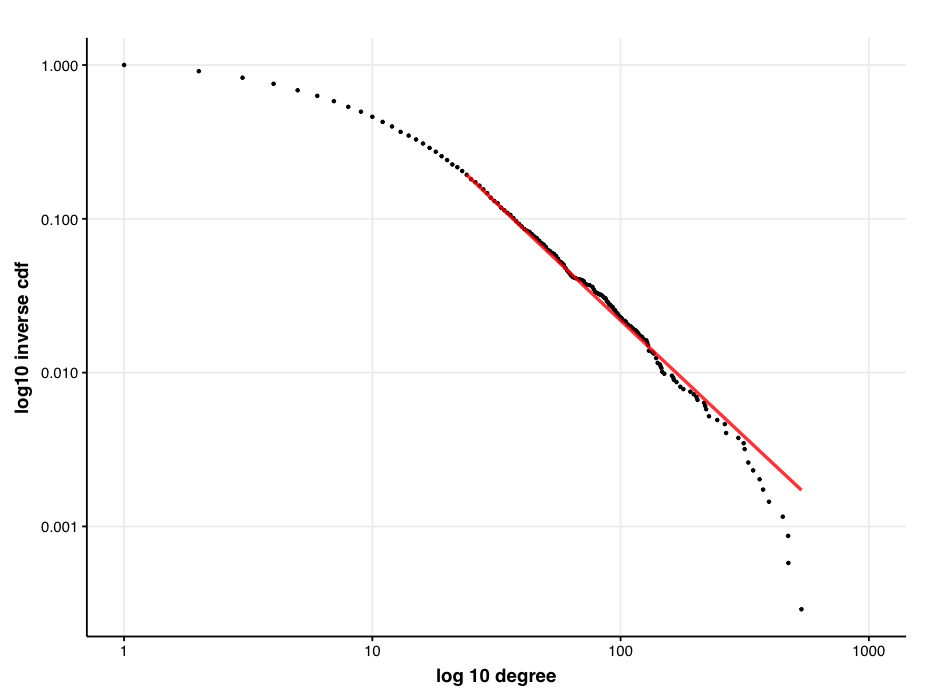
\includegraphics[width=\linewidth]{images/chapter3/ggplot2/theme/powerlaw/Rplot01_chapter3_cdf_and_powerlaw.png} 
        \caption{The plot of log cumulative cdf of degree distribution log 10 scale x and y. \textcolor{red}{this is 1 -cdf Actually see Newman on cdf complement}} \label{fig:log_degree_distribution}
    \end{subfigure}
    \caption{Plots of degree distribution}
    \label{fig:Plots of degree distribution}
\end{figure}
% latex table generated in R 3.4.4 by xtable 1.8-4 package
% Sat Oct  5 16:31:0\begin{document}



%Bootstrap p: power law 0.575

% bootstrap p log-normal 0.4
\begin{figure}
    \centering
    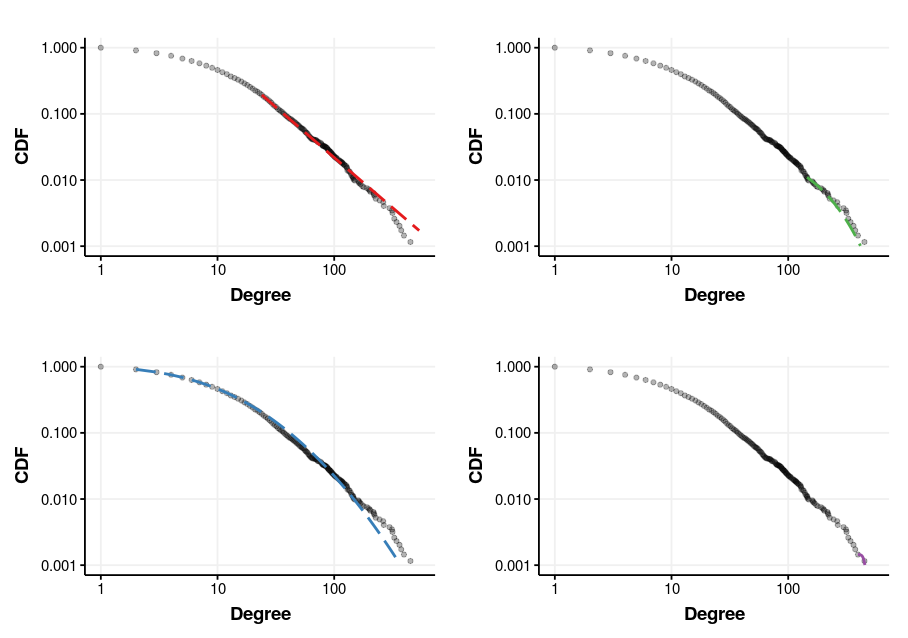
\includegraphics[width=\textwidth]{images/chapter3/poweRlaw/multiplot/Rplot_multiplot_with_x_min_each_distribution.png}
    \caption{FIT OVER ALL CDF of degree distribution and lines of best fit for power law (red), log-normal(blue) exponential(green) and poisson (purple). Poisson distribution is clearly a poor fit with x min close to x max (396) and the exponential distribution holds only in x min greater than 145. x axis degree log 10 scaled, y axis CDF log 10 scaled. Exponential appears a good fit but is fitted to a much smaller part of the distribution than the power law and log-normal. Poisson distribution is clearly not a good fit.}
    \small\url{source('~/RProjects/chapter3/R/fit_power_law/graphing/plot_power_law_and_lognormal_ggplot2_multiplot.R')}
    \label{fig:CDF degreel_multiplot}
\end{figure}
% p exponential < 0.01




% latex table generated in R 3.6.3 by xtable 1.8-4 package
% Sat Apr 17 12:56:22 2021
\begin{table}[ht]
\centering
\setlength{\extrarowheight}{2pt}
\begin{adjustbox}{width=\textwidth}

\begin{tabular}{lllllllll}
  \toprule
model & $LL$ & $p_{bs}$ & g.o.f & pars\textsubscript{1} & pars\textsubscript{2} & Vuong\textsubscript{statistic} & Vuong $p$\textsubscript{1} & Vuong $p$\textsubscript{2} \\ 
  \midrule
Power-law & -2943.61 & 0.57 & 0.02 & 2.511 &  & -1.32 & 0.906 & 0.0187 \\ 
  log-normal & -2941.56 & 0.38 & 0.01 & -2.345 & 2.11 & 1.32 & 0.094* & 0.0187 \\ 
  exponential & -3044.66 & $<0.001$ & 0.09 & 0.029 &  & 5.10 & $1.73 \times 10^{-7}$ & $3.46 \times 10^{-7}$ \\ 
  poisson & -14376.28 & $<0.001$ & 0.09 & 58.590 &  & 7.31 & $1.29 \times 10^{-13}$ & $2.58 \times 10^{-13}$ \\ 
   \bottomrule
\end{tabular}
\end{adjustbox}
\caption{Fit of distributions for PSP. Vuong test power law versus other test other than log-normal where one sided is log-normal versus power law marked with*. One sided test favours log-normal but not significantly so.} 
\tiny\url{source('~/RProjects/chapter3/R/fit_power_law/fit_pl_setxmin.R')}
\label{tab:Fit of distributions for PSP}
\end{table}


% latex table generated in R 3.6.3 by xtable 1.8-4 package
% Sat Apr 17 13:07:57 2021


\begin{figure}
    \centering
    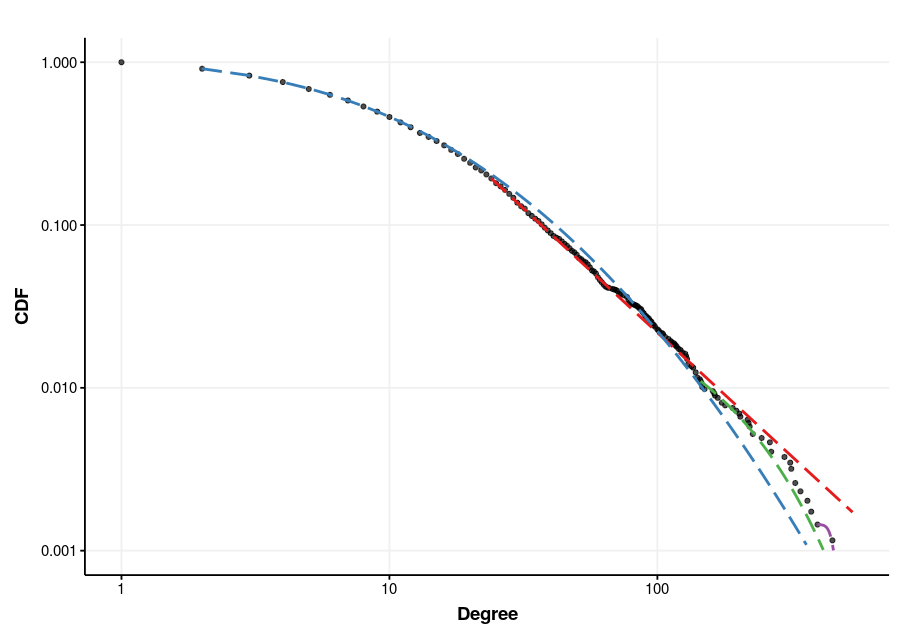
\includegraphics[width=\textwidth]{images/chapter3/poweRlaw/RPlot_plot_powerlaw_xmin_set_for_each_distribution_add_theme.png}
    \caption{FIT OVER ALL CDF of degree distribution and lines of best fit for power law (red), log-normal(blue) exponential(green) and poisson (purple). Poisson distribution is clearly a poor fit with x min close to x max (396) and the exponential distribution holds only in x min greater than 145. x axis degree log 10 scaled, y axis CDF log 10 scaled. Exponential appears a good fit but is fitted to a much smaller part of the distribution than the power law and log-normal. Poisson distribution is clearly not a good fit.} 
    \small\url{source('~/RProjects/chapter3/R/fit_power_law/graphing/plot_power_law_and_lognormal_ggplot2_add_theme.R')}
    \label{fig:CDF degreel_theme}
\end{figure}



\paragraph{free fit}



Figure~\ref{fig:CDF degreel_theme}(fit over whole distribution) shows that the Poisson distribution is a poor fit. The fit to the empirical distribution is poor fitting either the whole distribution or the portion for which a power law distribution holds (figure~\ref{fig:models_set_xmin}). \textcolor{red}{p bootstrap}.



\footnote{m pl x min 24
 
 Free fit ln xmin 2,Pars 2.120274 1.218815;
 
 Free fit exp xmin 145,pars = 0.008805921;
 
 Free fit poisson, x min 396, pars = 465.5668;
  basically puts all probability mass on 2 points\textcolor{red}{is this added to method if it comes out of footnotes}}
  .  

% The log-normal when not constrained over the 




% Power law LL
% -2943.606

% -2943.606

% Log normal LL
% -2941.556

% exp ll
% -3044.662

% poisson ll
% -180155.6


% Vuong 
% power law v log normal One sided p=0.906

% log normal v power law One sided p = 0.093

%     p two sided both above 0.187

% Compare power law and exponential one sided p = $1.72\times10^{-7}$
% power law and exponential two sided $3.455\times10^{-7}$


  \todo[inline]{add code and complete table}
  

  
\subsection{Global measures: Relationship of $C(k)$ to $k$}%\todo{is this needed?}
\label{sec:relationship of ck to k albert}
%\todo{add an introduction to this result and significance}
% You might want to start with another observed relationship is $C(k)$ and $k$ and I will expand on how $C_i$ depends on $k_{min}$ below.

In section~\ref{sec:correlation of centrality measures results section} all centrality measures are positively correlated yet mean local transitivity for nodes of degree $k$: $C(k)$, constant in random networks, is reported to decrease with increasing degree\cite{yook2004functional},\cite{albert2005scale} as,
\begin{equation}
            C(k) = \frac{B}{k^{\beta}},
\end{equation}
\label{eq:C(k) function average transitivity and degree}

 where $B$ is a constant and $\beta$ is typically between one and two\cite{albert2005scale},\cite{yook2004functional} in networks with hierarchical organisation. High degree nodes should have a lower mean transitivity and the relationship be roughly linear relationship when both axes are logarithmic. The relationship between $C(k)$ and degree $k$ in the PSP network  is shown in figure~\ref{fig:C(k)_doublelog}\footnote{Code \url{source('~/RProjects/graph2community/R/transitivity_degree/Cluster_nodes.R')}}.Initially $C(k)$ does not change with increasing degree but eventually $C(k)$ clearly decreases as $k$ increases. An almost exactly identical pattern is seen in\cite{yook2004functional}  (figure 2b) reporting the relationship in Eq(\ref{eq:C(k) function average transitivity and degree}). 

The overall correlation coefficient between degree and transitivity\textsubscript{NaN} is positive ($\rho= 0.196$; $p < 2.2 \times 10^{-16}$) and is higher when isolates are zero ($\rho$=0.375 for transitivity\textsubscript{0}). The reason for the difference between the positive correlation across the entire distribution and the relationship in figure~\ref{fig:C(k)_doublelog}) is the effect of nodes of degree one ($k=1$) and hence transitivity 0 - having very low degree and minimal transitivity hence highly correlated(figure~\ref{fig:Scatter plot of the relationship between degree and local transitivity for the PSP nodes}). The transitivity is also low for nodes of degree two.


\begin{figure}
    \centering
    \begin{subfigure}[t]{0.45\textwidth}
        \centering
        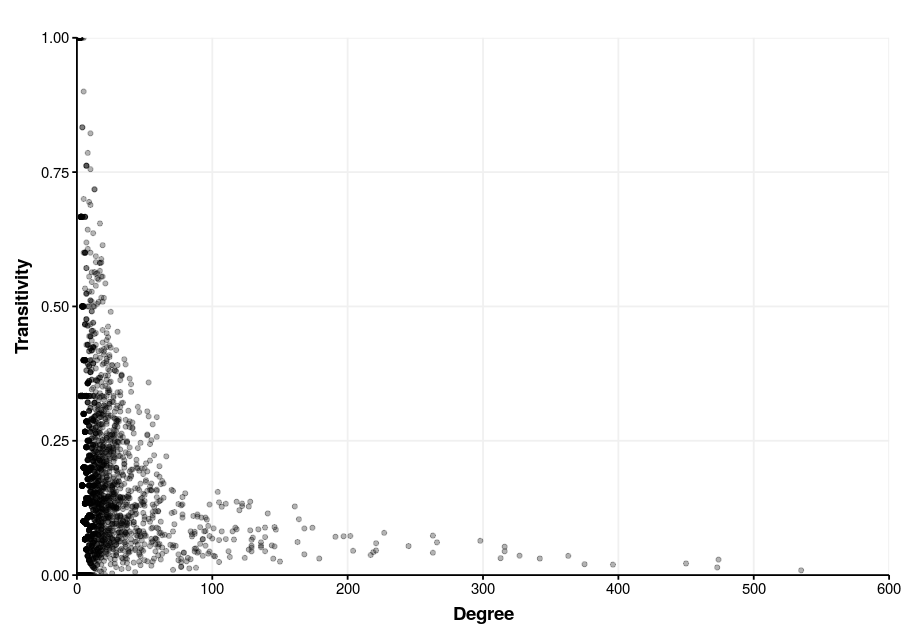
\includegraphics[width=\textwidth]{images/chapter3/ggplot2/degree_and_transitivity/Rplot_scatterplot_c_and_degree_new_format.png}
\caption{Scatter plot of the relationship between degree and local transitivity for the PSP nodes. Nodes with degree $k=1$ have transitivity zero. Plot appears to show a negative correlation between degree and transitivity. The opacity of points has been decreased to reduce overplotting and show the number of points of low degree. }
 \tiny\url{source('~/RProjects/chapter3/R/transitivity/transitivity_and_degree/mean_deg_seq.R')} plot p
    \label{fig:Scatter plot of the relationship between degree and local transitivity for the PSP nodes}
    \end{subfigure}
    \hfill
    \begin{subfigure}[t]{0.45\textwidth}
        \centering
        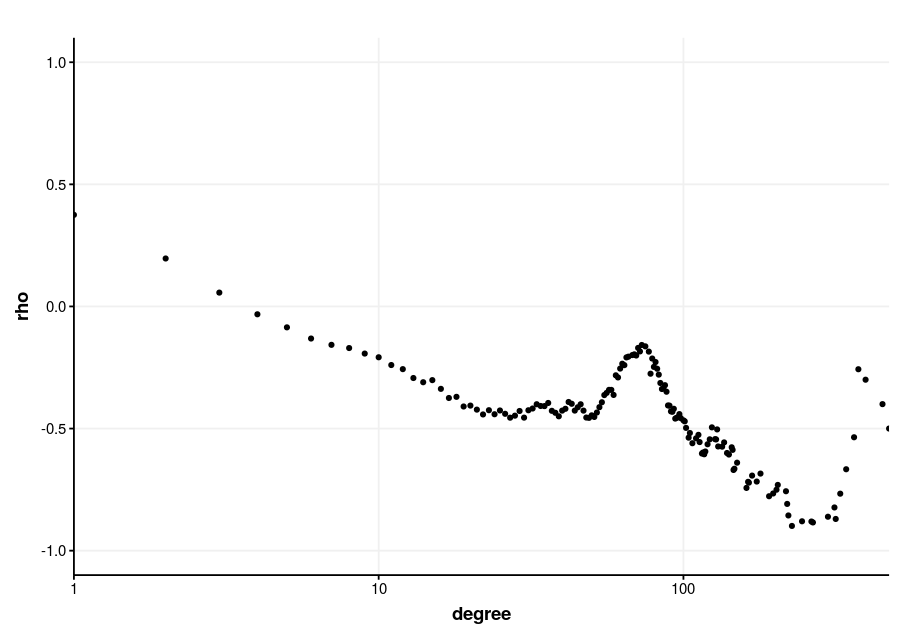
\includegraphics[width=\textwidth]{images/chapter3/ggplot2/degree_and_transitivity/Rplot_rho_and_starting_degree_transitivity.png}
        \caption{Plot of minumum degree included in the calculation of Spearmans rank correlation between degree and $\rho$. Although the overall coefficient is positive the correlation for nodes above degree 5 are clearly negative and this becomes more apparent at high degree. This relationship is therefore complex and the typical relationship described in the literature may only hold for the large networks in which this relationship has been studies such as the internet}.
    \tiny\url{source('~/RProjects/chapter3/R/transitivity/transitivity_and_degree/plot/plot_start_degree.R')}
    \label{fig:Plot of minumum degree included in the calculation of Spearmans rank correlation between degree and rho}
    \end{subfigure}
    \caption{$C(k)$ and $k_{min}$}
    \label{fig:Plots of degree distribution}
\end{figure}


For nodes with degree $k>=2$, $\rho$=0.196; $k>=3$ , $\rho$=0.056 and by $k>=5$ the correlation is negative ($\rho$=-0.085). The median degree is eight and five is the 0.369 quantile. The positive correlation between degree and transitivity found across all nodes is the result of the effect of the third of nodes with smallest degree (histogram of transitivity  see fig~\ref{fig:transitivity}). Plotting $\rho$ against the minimum degree included in calculating the correlation coefficient($k_{min})$ clearly shows the switch from positive to negative correlation between low degree and high degree regions (figure~\ref{fig:Plot of minumum degree included in the calculation of Spearmans rank correlation between degree and rho}).

The scaling described as being typical of hierarchical organisation is therefore seen clearly only when degree is above 5 and the relationship changes from a positive correlation in the low degree regime to the previously described scaling. In networks with large numbers of low degree node the correlation coefficient will not show this relationship and setting isolates to zero makes this positive correlation stronger(see discussion~\ref{sec:discuss degree and local transitivity - summary just now}) \footnote{although you don't see it if you use Pearson's correlation},\footnote{code \url{source('~/RProjects/centrality/R/transitivity/calculate_correlation_min_transitivity_and_plot.R', echo=TRUE)}}.



\subsection{Results Small world}

The small world effect is a combination of a high clustering coefficient and a short average path length(section~\ref{sec:small world methods})
\subsubsection{Global clustering coefficient}
\label{sec:results_global_clustering_coefficient}

The global clustering coefficient defined by Watts and Strogatz ($C_{WS}^0$) as the arithmetic mean of the vertex local clustering coefficients is 0.156 when isolates are set to zero\cite{watts1998collective} and 0.171 if the isolates are undefined and excluded ($C_{WS}^{NaN}$ - the default in igraph) is 0.171 (see above section~\ref{sec:Global clustering coefficient}). A histogram of local transitivity values is seen in figure~\ref{fig:transitivity}, although bounded in the region 0-1 the probability mass is concentrated on the left of the graph due to the number of nodes with low transitivity.

 The value of the global transitivity described by Newman ($C$ section~\ref{sec:global transitivity newman}) is 0.070. The different global transitivity measures are reviewed in table~\ref{tab:Different global transitivities in igraph}.


% latex table generated in R 3.6.3 by xtable 1.8-4 package
% Sat Feb 20 12:04:47 2021
\begin{table}[ht]
\centering
\begin{adjustbox}{width=\textwidth}
\begin{tabular}{llllc}
  \toprule
Name & Symbol &  type & isolates & Global Transitivity \\ 
  \midrule
Watts-Strogatz & $C_{WS}^{0}$& `localaverageundirected'CHECK
 &isolates=`zero' & 0.156\vspace{1mm} \\ 

Watts-Strogatz & $C_{WS}^{NaN}$ &`globalaverageundirected'*&isolates=`NaN' & 0.171\vspace{1mm} \\ 
  Newman &$C$&`globalundirected' &isolates=`zero'& 0.070\vspace{1mm} \\ 
  Newman &$C$&`globalundirected'&isolates=`NaN'& 0.070 \\ 
   \bottomrule
\end{tabular}
\end{adjustbox}
\caption[Different global transitivities in igraph]{Different global transitivities in igraph. * or mean of `localundirected' with isolates `NaN' 
\tiny\url{source('~/RProjects/chapter3/R/transitivity/global_transitivity/global_transitivity.R')} 
\tiny same project \url{R/transitivity/global_transitivity/mkdown/global_transitivity_markdown.html}} 
\label{tab:Different global transitivities in igraph}
\end{table}


% % latex table generated in R 3.6.1 by xtable 1.8-4 package
% % Wed Mar 10 19:35:16 2021
% \begin{table}[ht]
% \centering
% \begin{tabular}{rrrrrrrrrrr}
%   \hline
%  & Min. & 1st Qu. & Median & Mean & 3rd Qu. & Max. & PSP & difference & sd & n\_sd \\ 
%   \hline
% C Newman & 0.005 & 0.005 & 0.005 & 0.005 & 0.005 & 0.006 & 0.070 & 0.065 & 1.712E-04 & 377.5 \\ 
%   C\_WS\_NAN & 0.005 & 0.005 & 0.005 & 0.005 & 0.005 & 0.006 & 0.171 & 0.166 & 1.816E-04 & 915.4 \\ 
%   C\_WS\_0 & 0.005 & 0.005 & 0.005 & 0.005 & 0.005 & 0.006 & 0.156 & 0.151 & 1.816E-04 & 832.4 \\ 
%   \hline
% \end{tabular}
% \caption{Global transitivity Monte Carlo Erdos Renyi\url{source('~/RProjects/chapter3/R/transitivity/global_transitivity/monte_carlo_er_global_transitivity.R')}}
% \end{table}
% \paragraph{This bit is all about local transitivity}
% The expected value of mean local clustering given a random rewiring with fixed degree distribution is 0.07479691 sd (0.00183) removing NA and 0.068 setting NA to 0 (100 iterations) and 0.0682 seeting NA to zero with sd 0.00181 \footnote{Code  \url{source('~/RProjects/centrality/R/transitivity/calculate_local_transitivity_and_simulate_mean.R')} }


% latex table generated in R 3.6.1 by xtable 1.8-4 package
% Wed Mar 10 19:39:04 2021
% \begin{table}[ht]
% \centering
% \begin{tabular}{rrrrrrrrrrr}
%   \hline
%  & Min. & 1st Qu. & Median & Mean & 3rd Qu. & Max. & PSP & difference & sd & n\_sd \\ 
%   \hline
% C Newman & 0.055 & 0.058 & 0.058 & 0.058 & 0.059 & 0.061 & 0.070 & 0.011 & 8.032E-04 & 14.2 \\ 
%   C\_WS\_NAN & 0.069 & 0.073 & 0.075 & 0.075 & 0.076 & 0.081 & 0.171 & 0.097 & 1.981E-03 & 48.8 \\ 
%   C\_WS\_0 & 0.063 & 0.067 & 0.068 & 0.068 & 0.069 & 0.074 & 0.156 & 0.088 & 1.807E-03 & 48.8 \\ 
%   \hline
% \end{tabular}
% \caption{Global transitivity Monte Carlo configuration model \url{source('~/RProjects/chapter3/R/transitivity/global_transitivity/monte_carlo_er_global_transitivity.R')}}
% \end{table}

% latex table generated in R 3.6.3 by xtable 1.8-4 package
% Thu Mar 11 17:41:34 2021
The global transitivity values compared to Monte Carlo estimates using Erdos Renyi random graphs with the same number of edges and nodes as the PSP (table~\ref{tab:MC estimate of ER transitivity}). The Watts-Strogatz transitivity is larger than the Newman transitivity (0.156 vs 0.70). It is not clear what the significance of the divergence in values is \cite{newman2018networks} but it is absent in the random graphs and appears to be a feature of the network. The absolute size of the difference between the PSP and ER transitivity is small but is of the order of several standard deviations (377.5 for Newman Transitivity) and the samples of the ER transitivity appear normally distributed (see KS in table~\ref{tab:MC estimate of ER transitivity}).


\begin{table}[ht]
\centering
\begin{adjustbox}{width=\textwidth}
\begin{tabular}{llllllllll}
  \toprule
 & Median ER & Mean ER & PSP & difference & sd & $n$ sd & ks $d$ & ks $p$ & $p$ \\ 
  \midrule
$C$ & $5.096 \times 10^{-3}$ & $5.106 \times 10^{-3}$ & 0.070 & 0.065 & $1.712 \times 10^{-4}$ & 377.5 & 0.026 & 0.51 & 0 \vspace{1mm} \\ 
  $C_{WS}^{NaN}$ & $5.095 \times 10^{-3}$ & $5.104 \times 10^{-3}$ & 0.171 & 0.166 & $1.816 \times 10^{-4}$ & 915.4 & 0.024 & 0.63 & 0 \vspace{1mm} \\ 
  $C_{WS}^0$ & $5.095 \times 10^{-3}$ & $5.104 \times 10^{-3}$ & 0.156 & 0.151 & $1.816 \times 10^{-4}$ & 832.4 & 0.024 & 0.63 & 0 \vspace{1mm}\\ 
   \bottomrule
\end{tabular}
\end{adjustbox}
\caption[Global transitivity of PSP and Monte Carlo estimates - Erdos-Renyi]{The global transitivity measures of the PSP are compared with Monte Carlo estimates of the transitivity measures in Erdos Renyi random graphs with matching numbers of vertices and edges. 1000 iterations. difference  = PSP - mean Monte Carlo Estimate $n$ sd number of times difference greater than standard deviation of MC estimate mean. ks $d$ = Kolmogorov-Smirnov statistic distance,ks $p$ Kolmogorov-Smirnov test statistic comparing Monte Carlo estimate to normal distribution with identical mean and standard deviation,  $p$ probability of result as extreme as PSP using mean and standard deviation of MC estimates.} \tiny\url{source('~/RProjects/chapter3/R/transitivity/global_transitivity/monte_carlo_er_global_transitivity.R')} 
\label{tab:MC estimate of ER transitivity}
\end{table}


Monte Carlo estimates of the transitivity in the degree constant configuration model are shown in table~\ref{tab: MC estimate of config transitivity}. There is less difference between the PSP transitivity and the Configuration model than between the PSP and the ER graphs in both absolute terms or in the number of standard distributions it represents. The Watts-Strogatz global transitivity is again differs most from the random model. There is a difference in the value of the mean transitivity between the different types of transitivity with their rank order being the same as the PSP (Watts-Strogatz is greatest). I would hypothesise some but not all of the divergence in these values (WS and Newman) are due to degree structure but the divergence appears to be a feature of real world graphs. 

The global undirected transitivity of the PSP network is 0.0697. This is similar to the value reported by Newman\footnote{p305} \cite{newman2018networks} in metabolic networks (0.090) and PPI (0.072).
% latex table generated in R 3.6.3 by xtable 1.8-4 package
% Sat Mar 13 14:48:46 2021
\begin{table}[ht]
\centering
\begin{adjustbox}{width=\textwidth}


\begin{tabular}{llllllllll}
  \toprule
 & Median Config & Mean & PSP & difference & sd & $n$ sd & ks $d$ & ks $p$ & $p$ \\ 
  \midrule
$C$  & $5.835 \times 10^{-2}$ & $5.836 \times 10^{-2}$ & 0.070 & 0.011 & $8.032 \times 10^{-4}$ & 14.2 & 0.016 & 0.95 & 0 \\ 
   $C_{WS}^{NaN}$  & $7.475 \times 10^{-2}$ & $7.480 \times 10^{-2}$ & 0.171 & 0.097 & $1.981 \times 10^{-3}$ & 48.8 & 0.024 & 0.63 & 0 \\ 
   $C_{WS}^0$ & $6.818 \times 10^{-2}$ & $6.822 \times 10^{-2}$ & 0.156 & 0.088 & $1.807 \times 10^{-3}$ & 48.8 & 0.024 & 0.63 & 0 \\ 
   \bottomrule
\end{tabular}
\end{adjustbox}
\caption[Transitivity PSP compared with configuration model]{PSP vs 1000 Configuration model Monte Carlo. 1000 iterations. difference  = PSP - mean Monte Carlo Estimate $n$ sd number of times difference greater than standard deviation of MC estimate mean. ks $d$ = Kolmogorov-Smirnov statistic distance,ks $p$ Kolmogorov-Smirnov test statistic comparing Monte Carlo estimate to normal distribution with identical mean and standard deviation,  $p$ probability of result as extreme as PSP using mean and standard deviation of MC estimates. }
\tiny\url{source('~/RProjects/chapter3/R/transitivity/global_transitivity/monte_carlo_config2_global_transitivity.R')}
\label{tab: MC estimate of config transitivity}
\end{table}


\cite{newman2003social}
\cite{vasques2020transitivity}



    
\begin{figure}
    \centering
    \begin{subfigure}[t]{0.45\textwidth}
        \centering
        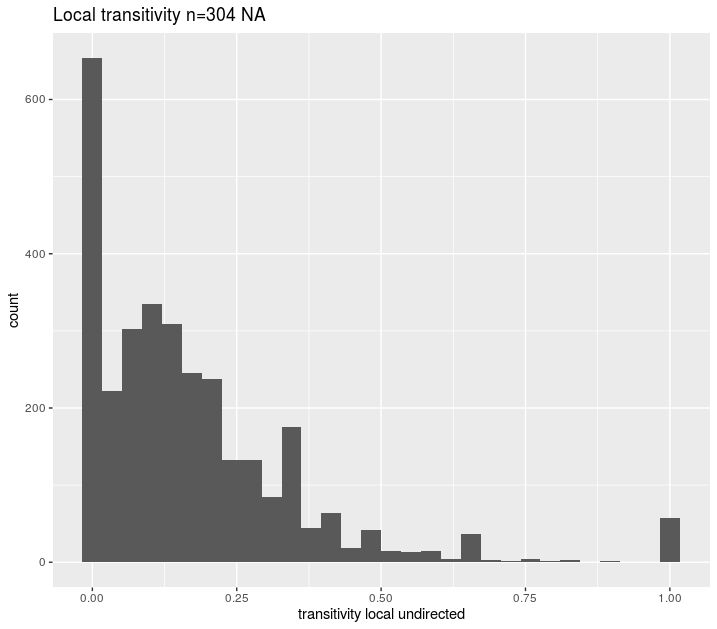
\includegraphics[width=\linewidth]{images/Rplot_transitivity.png} 
        \caption{Histogram of transitivity} \label{fig:transitivity}
    \end{subfigure}
    \hfill
    \begin{subfigure}[t]{0.45\textwidth}
        \centering
        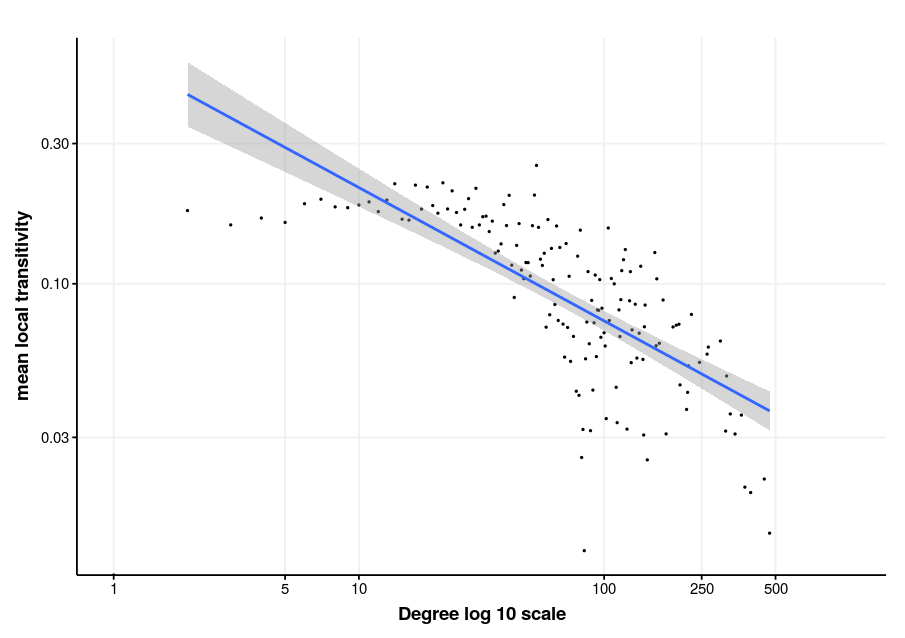
\includegraphics[width=\linewidth]{images/chapter3/ggplot2/c(k)/Rplot_C_k_new_formatted.png}
        %{images/Rplot01_logdegree_log_transitivity.png} 
        \caption{Plot of degree with mean local transitivity. Log10-log10 scale. Omitting degree $k=1$ as transitivity $C$ will be undefined.} \label{fig:log_transitivity_degree}
    \end{subfigure}
    \caption{Plots of transitivity \textcolor{red}{may want to do this in subfigure packages rather than subcaption to line up edges}}
\end{figure}


\subsubsection{Results: Average path length and transitivity}
\label{sec:Results average path length and transitivity}

We have dealt with the results for the global clustering coefficient we also need to determine the average path length in order to investigate the small world phenomenon. The average path length of the PSP was again compared Monte Carlo estimates of the average path length for the Erdos Renyi models and configuration models.

The average path length was shortest for the PSP (2.98) and longest for the Erdos Renyi graph with the Configuration Model again in the middle. The value for one sample t tests of the difference between the Monte Carlo estimates and the PSP are in \url{source('~/RProjects/chapter3/R/transitivity/global_transitivity/t_test/compare_er_config.R')}.

The average path length calculated using the \texttt{mean\_distance} function in igraph is 2.98. Global (not WS) transitivity 0.0697.

Maybe you want to do the table like~\ref{tab:small world apl and c}
\begin{table}[]
    \centering
    \begin{tabular}{llllll}
    \toprule
    Graph     &  APL & sd & $C_{WS}$& $C_{WS}0$ & $C$ \\
    \midrule
    PSP     & 2.98 & NA & 0.171 & 0.156 & 0.0697 \\
    ER      & 3.118 & 0.00047 & 0.0051 & 0.0051 & 0.0051 \\
    Config  & 3.0069 &0.0053& 0.0683 & 0.0748 & 0.0584\\
    \bottomrule
    \end{tabular}
    \caption{Alternative way of presenting the data take transitivity from PSP vs 1000 Configuration model Monte Carlo
    \tiny\url{source('~/RProjects/chapter3/R/transitivity/global_transitivity/monte_carlo_config2_global_transitivity.R')}}
    \label{tab:small world apl and c}
\end{table}




For the degree corrected configuration model see table~\ref{tab:cmtransitivity_configuration_model} \textcolor{red}{cross ref with albert should have shorter average path length}. The average path length is shorter than in the Erdos Renyi model likely due to the presence of hub nodes\footnote{ Code \url{source('~/RProjects/graph_sw/R/small_world_random/degree_corrected_config_random_ws.R')}}.


This is similar to the L of 2.65 and C of 0.28 of C elegans, where L is the ``shortest path between two vertices, averaged over all pairs of vertices and C is the clustering coefficient'' as defined by Watts and Strogatz \cite{watts1998collective}. The random rewiring with a uniform probability leads to a L of 3.11. \todo{add table of path length} See table~\ref{tab:clustering and path length Watts and Strogatz}


\begin{table}[h]
    \centering
    \begin{tabular}{lllll}
    \toprule
    Network      & L\textsubscript{actual} & L\textsubscript{random} & C\textsubscript{actual} & C\textsubscript{random} \\
    \midrule
     Film actors    & 3.65 & 2.99 & 0.79 & 0.00027\\
     Power grid & 18.7 & 12.4 & 0.080 & 0.005 \\
     \textit{C elegans} & 2.65 & 2.25 & 0.28 & 0.05 \\
     \bottomrule
    \end{tabular}
    \caption{Clustering coefficient and average path length of three networks compared to random Erdos Renyi graph with same number of nodes and edges - from Watts and Strogatz\cite{watts1998collective}. $L$ is average path length, $C$ is global transitivity of type Watts-Strogatz\textcolor{red}{add n - ? scales wih n add psp for comparison comment all have actual greater than random}}
    \label{tab:clustering and path length Watts and Strogatz}
\end{table}

\todo{add omnigenic bit}%see code source('~/RProjects/graph_transitivity/R/transitivity.R')

% latex table generated in R 3.6.3 by xtable 1.8-4 package
% Sat Mar 13 15:45:33 2021
\begin{table}[ht]
\centering
\begin{adjustbox}{width=\textwidth}

\begin{tabular}{rrrrrrrrrr}
  \toprule
 & Median & Mean & PSP & difference & sd & n\_sd & ks\_d & ks\_p & p \\ 
  \midrule
APL & 3.01 & 3.01 & 2.980 & -0.027 & $5.304 \times 10^{-3}$ & -5.2 & 0.017 & 0.93 & 1 \\ 

   \bottomrule
\end{tabular}
\end{adjustbox}
\caption{PSP vs 1000 Configuration model Monte Carlo} 
\end{table}


% latex table generated in R 3.6.3 by xtable 1.8-4 package
% Sat Mar 13 16:16:30 2021
\begin{table}[ht]
\centering
\begin{adjustbox}{width=\textwidth}
\begin{tabular}{lllllllllll}
  \toprule
 & Median & Mean & CI& PSP & difference & sd & n\_sd & ks\_d & ks\_p & p \\ 
  \midrule
APL & 3.12 & 3.12 & 2.980 &3.1179-3.1180 & -0.138 & $4.875 \times 10^{-4}$ & -283.5 & 0.028 & 0.43 & $<2.2 \times 10^{-16}$ \\ 
 
   \bottomrule
\end{tabular}
\end{adjustbox}
\caption{PSP vs 1000 ER model Monte Carlo} 
\end{table}




 
 
 % latex table generated in R 3.6.3 by xtable 1.8-4 package
% Sat Mar 13 16:59:18 2021
\begin{table}[ht]
\centering
\begin{adjustbox}{width=\textwidth}
\begin{tabular}{lrrrrrrll}
  \toprule
 & estimate & t-statistic & p.value & d.f & conf.low & conf.high & method & alternative \\ 
  \midrule
t-test APL ER & 3.118 & 8964.21 &    0 & 999 & 3.1180 & 3.1180 & One Sample t-test & two.sided \\ 
   \bottomrule
   
\end{tabular}
\end{adjustbox}
\caption{T test APL ER\url{source('~/RProjects/chapter3/R/small_world/average_path_length/monte_carlo_er_apl.R')}}
\end{table}


\subsubsection{Distance distribution}

To test for the presence of the small world effect Barabasi recommends comparing the distance distribution (pairwise distances between all nodes) with the Erdos Renyi graph and the configuration model. This is essentially using all of the path lengths that make up the average path length to have a distribution of values for the PSP to compare to a random model.

The results show that the PSP has the a significantly shorter mean path length (this is just average path length with all the data that made it up) compared to the other two. The configuration model has a shorter path length than the ER model but longer than the PSP. This is in keeping with our other results (though not those suggested by Barabasi) - tables~\ref{tab:ANOVA_distance_distribution} and table~\ref{tab:Tukey post hoc}. Infinite values have been removed from the random graphs (distance values are infinite when the graph is disconnected).

The results support the PSP having a small world configuration. 

% latex table generated in R 3.6.1 by xtable 1.8-4 package
% Mon Mar 22 16:22:45 2021
\begin{table}[ht]
\centering
\begin{tabular}{lrrrrr}
  \toprule
 & Df & Sum Sq & Mean Sq & F value & Pr($>$F) \\ 
  \midrule
Graph types & 2 & 64211.02 & 32105.51 & 81460.66 & 0.0000 \vspace{1mm}\\ 
  Residuals & 17921085 & 7063109.61 & 0.39 &  &  \vspace{1mm}\\ 
   \bottomrule
\end{tabular}
\caption{ANOVA (aov in R) of distance distribution of PSP, Erdos Renyi Graph and Configuration model. Erdos-Renyi with n,m matching PSP. Configuration uses degree distribution of PSP}
\tiny\url{source('~/RProjects/chapter3/R/small_world/distance_distribution/barabasi_distance_distribution.R')}
\label{tab:ANOVA_distance_distribution}
\end{table}
% latex table generated in R 3.6.1 by xtable 1.8-4 package
% Mon Mar 22 15:04:39 2021
\begin{table}[ht]
\centering
\begin{tabular}{rrrrr}
  \toprule  
 & diff & lwr & upr & p adj \\ 
  \midrule
ER-PSP & 0.139 & 0.138 & 0.140 & $<0.001$ \\ 
  Config-PSP & 0.024 & 0.023 & 0.025 & $<0.001$ \\ 
  Config-ER & -0.115 & -0.116 & -0.114 & $<0.001$ \\ 
   \bottomrule
\end{tabular}
\caption[Tukey Distance Distribution]{Post hoc  Tukey multiple comparisons of means
    95\% family-wise confidence level Distance Distribution. p is 0. Diff= difference in means. Mean pairwise distance $n$=5,973,696 for PSP, Erdos Renyi gnm graph with identical $n$ vertices and edges to PSP and configuration random graph using PSP degree distribution. }
\tiny\url{source('~/RProjects/chapter3/R/small_world/distance_distribution/barabasi_distance_distribution.R')}
\label{tab:Tukey post hoc}
\end{table}



\paragraph{Small worldness measure}
The the small world measure $S$ where a graph is small world if $S>1$ \cite{humphries2008network} is 14.3\footnote{\url{source('~/RProjects/chapter3/R/small_world/calculate_humphries_small_world_metric.R')}}.
Using the definition of small worldness from Humphries and Gurney.

The measure of small worldness $S$ is $S>1$ for small world networks:

\begin{equation}
    \gamma_g = \frac{C_g}{C_{random}}
\end{equation}

and

\begin{equation}
    \lambda_g = \frac{C_g}{C_{random}}
\end{equation}


then

\begin{equation}
    S = \frac{\gamma}{\lambda}
\end{equation}

S global =  14.3\footnote{\url{source('~/RProjects/chapter3/R/small_world/calculate_humphries_small_world_metric.R')}}

S Watts Strogatz = 35.08\footnote{\url{source('~/RProjects/chapter3/R/small_world/calculate_humphries_small_world_metricWS.R')}}

A value greater than one is defined as denoting the small world property\cite{humphries2008network}. Thirty three real world networks showed a range of values from   1.34 (student relationships) ~11660 for math coauthorship (Newman method)  and for WS 0.27 student relationship (not small world) to 61967 for biology co-authorship n=11,803,064. They found that $S$ scaled linearly with $n$ the number of vertices in thenetwork. Linear regression on the log transform \textcolor{red}{of what presumably $S$ on $n$} yielded $0.023n^{0.96}$.

The predicted value for the PSP is is 57.39 ($\Delta$ ie not WS) and for $S$ using WS Sws=$0.012n^{1.11}$ = 101.65 
although the actual values in the table sometimes have WS greater than delta \textcolor{red}{?}. There is also a typo in the yeast average degree. 


\paragraph{Conclusion} The network shows the small world property. It is less than theoretical maximum small world and behaves similarly to other networks in its scaling with n. There is a wide variation to the small worldness\footnote{Humphries uses Small-Worldness but other authors Colon-Perez use worldness} of real world networks that have the small world property. 



\clearpage

\subsection{RESULTS Global  Assortativity and methods degree assortativity}
\subsubsection{Degree Assortativity}


 The PSP network is disassortative (methods section~\ref{sec:Assortativity methods}) with regard to degree ($\rho_D$=-0.18)\footnote{using the notation in Noldus\cite{noldus2015assortativity}},\footnote{using the commands \texttt{assortativity(g,deg,directed=FALSE)} in igraph for R}. 
 This value  \todo{three sf} is similar to those reported in biological networks including yeast protein-protein interaction networks (-0.156) and neural networks (-0.163) \cite{newman2002assortative}  and summarised in table~\ref{Table:DegreeAssortativityNewman}. Amongst non biological networks it is most similar in magnitude to that of the internet in 2002\cite{newman2002assortative} ($r=$-0.189). 

 A Monte Carlo estimate of the expected value of the degree assortativity for the configuration model with identical degree sequence is very close to zero: -0.00003 (10,000 iterations ; min. -0.022, max.  0.026). The degree assortativity is far from what would be expected by chance  $p_{MC}<0.0001$\footnote{\url{source('~/RProjects/chapter3/R/assortativity_distribution/assortativity_config.R')}}.

The degree assortativity is negative in most real world networks other than social networks \cite{newman2002assortative}  ( table \ref{Table:DegreeAssortativityNewman})\todo{? add positive $r$ to table}. The random model is known to have zero correlation although low values ($r<0.02$) may be due to chance)\cite{noldus2015assortativity}). A standard (Barabsi-Albert) generative model for scale free networks is  mildly disassortative\cite{noldus2015assortativity} when small but also shows no degree assortativity in the limit of large $n$\cite{noldus2015assortativity}. \footnote{This is at odds with our later finding (see orthologues) that nodes with clearly identified yeast orthologues tend to be of higher degree (this would fit both the Barabasi Albert model and Callaway)} 
%\todo{this is the bit where the pseudohub bit would fit}. XX

The assortativity suggests that the Barabasi-Albert model is `incomplete' as a model of the internet \cite{newman2002assortative} and by extension the PSP protein-protein interaction network and would need to be accounted for in construction probabilistic models of the network\footnote{there are other things in our study that support the Barabasi model and it may be that multiple processes are taking place}. 
The Callaway model of network generation ('grown graph' - newman\footnote{Noldus distinguishes between grown graphs such as the Callaway and Barabasi-Albert and evolving graphs such as the Watts-Strogatz generative model}) shows the positive degree correlation seen in social networks but is inaccurate as a model of other complex networks (including online social networks). 


\begin{table}[]
    \centering
    \begin{tabular}{lll}
    \toprule
       network  &N& $r$  \\
       \midrule
       internet & 10697&-0.189\\
       world wide web &269504 & -0.065\\
       post synaptic proteome & 3457 & -0.18\\
       protein interactions & 2115 & -0.156\\
       neural network & 307 & -0.163\\
       food web & 92 & -0.276 \\
       \bottomrule
    \end{tabular}
    \caption{Degree assortativity coefficients of networks adapted from Newman 2002 \cite{newman2002assortative} including post synaptic proteome}
    \label{Table:DegreeAssortativityNewman}
\end{table}

%\subsubsection{Degree correlation}
 
\todo{Include \url{R_plot_degree_correlation.png} commented out}

Clustering and interconnection of communities tends to lead to higher assortativity by degree and branching negative\cite{estrada2011combinatorial}\cite{noldus2015assortativity}. Higher assortativity in social networks leads to higher modularity and clustering coefficient\cite{noldus2015assortativity}. Community formation is more remarkable therefore in overall disassortative networks. 

% This is possibly the bit where Keith's bit would be good to put in.  
 %\begin{figure}]h]
 % \includegraphics[width=\linewidth]{Rplot_degree_correlation.png}
 % \caption{Plot of degree with k nearest neighbour mean of degree}
 % \label{fig:knn_degree}
%\end{figure}
%
%
%
\subsubsection{Assortativity other centrality measures}

% latex table generated in R 3.6.3 by xtable 1.8-4 package
% Sat Feb 27 12:16:57 2021

Table~\ref{tab:assortativity by centrality} shows that the network is most disassortativty by degree. By contrast kcoreness and closeness are assortative suggesting a central area of genes (core) that are more highly connected\footnote{\url{source('~/RProjects/chapter3/R/assortativity_distribution/centrality/assortativity_by_centrality.R')}}. An accurate probabilistic generative model would also need to take this into consideration.  

\begin{table}[ht]
\centering
\begin{tabular}{lr}
  \toprule
Centrality measure & assortativity ($\rho$) \\ 
  \midrule
kcoreness & 0.089 \\ 
  Closeness & 0.072 \\ 
  Eigenvector & -0.033 \\ 
  Transitivity0 & -0.036 \\ 
  Betweenness & -0.093 \\ 
  Degree & -0.178 \\ 
   \bottomrule
\end{tabular}
\caption{Assortativity by centrality measure.}
\tiny\url{source('~/RProjects/chapter3/R/assortativity_distribution/centrality/assortativity_by_centrality.R')} 
\label{tab:assortativity by centrality}
\end{table}


\subsubsection{Assortativity and gene score}

 The guilt by association hypothesis (section~\ref{sec:Assortativity methods}) suggests that similar genes are linked. We can test whether genes associated with intelligence or educational attainment in the sample GWAS ore more likely to be linked considering the network as a whole by calculating the assortativity of the network by study z score provided by MAGMA (as we are interested in correlation rather than the absolute values - see discussion). 
 
 Some genes in the PSP do not have SNPs within them that appear in the study samples and therefore  not have a Z score assigned by MAGMA. These missing values are set to zero or the median value of the z-score (to ensure there is no significant difference between either strategy) as the assortativity function does not accept missing values\footnote{code \url{source('~/RProjects/centrality/R/get_gene_scores/assortativity_with_z_scores.R')} },
\footnote{Redo \url{source('~/RProjects/chapter3/R/assortativity_distribution/z_score/assortativity_z.R', echo=TRUE)}}. 

\subsubsection{Assortativity with z score results}
 
 There is no evidence that across the PSP nodes are assortative or disassortative by the level of association of gene Z scores for studies of intelligence or educational attainment. 
 \todo[inline]{random assortativity equal n probably sample from z scores}
 

\begin{table}[]
     \centering
     \begin{tabular}{llllll}
     \toprule
         Study & Missing values  & Assortativity\textsubscript{0} & Assortativity\textsubscript{median} & p\textsubscript{BS 0} & p\textsubscript{BS median}\\
         \midrule
         Intelligence\textsubscript{Replication} & 148 & 0.003 & 0.0032 & 0.78 & 0.79\\
         Education\textsubscript{Replication} & 172 & -0.006 &  -0.0064&0.20 & 0.18 \\ 
         Education\textsubscript{Discovery} & 156 & 0.001 & -0.0002&0.67 & 0.59\\
         Intelligence\textsubscript{Discovery} & 156 & -0.004 & -0.0038&0.31 & 0.33\\
         \bottomrule
     \end{tabular}
     \caption{Assortativity of PSP graph vertices by study Z score. PSP graph members without corresponding Z score marked as missing values had z set to either 0 (Assortativity\textsubscript{0} or the median z score Assortativity\textsubscript{median}for missing set to zero \url{source('~/RProjects/centrality/R/get_gene_scores/assortativity_with_z_scores.R')} . All values not significantly different ($p>0.05$) than bootstrap estimate of assortativity (\url{source('~/RProjects/chapter3/R/assortativity_distribution/bootstrap/bootstrap_zscore_assortativity_studies.R')}}
     \label{tab:Assortativity of PSP graph and z scores1}
 \end{table}

 
 


% latex table generated in R 3.6.3 by xtable 1.8-4 package
% Sun Mar 14 14:30:44 2021

The results are shown in table~\ref{tab:Assortativity of PSP graph and z scores1} (and supplemental table~\ref{tab:Assortativity of PSP graph and z scores}) missing values have been assigned value 0 (Assortativity\textsubscript{0}) or the median z score (Assortativity\textsubscript{median}) as the nominal assortativity function in igraph requires values for all vertices. Assortativity scores tend to me modest (as score of approximately 0.15 is often found for degree assortativity).  These results are close to zero and do not differ from what could be expected by chance 

This suggests that nodes with high or low z scores in the population cohorts are no more likely to have links to one another \textit{globally} across the network. It does not state that there cannot be areas within the graph where there are areas of high assortativity or areas where one high score connects to linker node connects to another high score in a group.

\subsubsection{Assortativity with murine LTP}

% % latex table generated in R 3.6.3 by xtable 1.8-4 package
% % Mon Feb 22 17:39:30 2021
% \begin{table}[ht]
% \centering
% \begin{tabular}{llr}
%   \hline
% MP & Name & Q \\ 
%   \hline
% MP0001463 & abnormal spatial learning & 0.045 \\ 
%   MP0001468 & abnormal temporal memory & 0.029 \\ 
%   MP0001469 & abn context condition & 0.030 \\ 
%   MP0001473 & reduced long term potentiation & 0.025 \\ 
%   MP0001898 & abnormal long term depression & 0.063 \\ 
%   MP0002062 & abn assoc learning & 0.042 \\ 
%   MP0002062 & abormal associative learning & 0.042 \\ 
%   MP0002063 & abnormal learning memory conditioning & 0.053 \\ 
%   MP0004859 & abnormal synaptic plasticity & 0.049 \\ 
%   MP0014114 & abnormal cognition & 0.053 \\ 
%   \hline
% \end{tabular}
% \caption{Nominal assortativity for mammalian phenotypes. and $n$ and $ci$ Source \url{source('~/RProjects/chapter3/R/assortativity_distribution/nominal_murine/2_Feb_murine_LTP_assortativity.R')}} 
% \label{tab:Nominal assortativity for mammalian phenotypes}
% \end{table}


\begin{table}[ht]
\centering
\setlength{\extrarowheight}{2pt}
\begin{adjustbox}{width=\textwidth}


\begin{tabular}{lllllll}
  \toprule
MP & Name & n & $Q$ & max Q\textsubscript{MC} & $\mu_Q$ MC & $p$ \\ 
  \midrule
MP0001463 & abnormal spatial learning & 272 & 0.045 & 0.022 & -0.001 & $<0.0001$ \\ 
  MP0001468 & abnormal temporal memory & 215 & 0.029 & 0.021 & -0.001 & $<0.0001$ \\ 
  MP0001469 & abn context condition & 181 & 0.030 & 0.020 & -0.001 & $<0.0001$ \\ 
  MP0001473 & reduced long term potentiation & 172 & 0.025 & 0.021 & -0.001 & $<0.0001$ \\ 
  MP0001898 & abnormal LTDep & 102 & 0.063 & 0.024 & -0.001 & $<0.0001$ \\ 
  MP0002062 & abn assoc learning & 339 & 0.042 & 0.021 & -0.001 & $<0.0001$ \\ 
  MP0002062 & abormal associative learning & 339 & 0.042 & 0.018 & -0.001 & $<0.0001$ \\ 
  MP0002063 & abnormal learning memory conditioning & 742 & 0.053 & 0.020 & -0.001 & $<0.0001$ \\ 
  MP0004859 & abnormal synaptic plasticity & 77 & 0.049 & 0.025 & -0.001 & $<0.0001$ \\ 
  MP0014114 & abnormal cognition & 744 & 0.053 & 0.020 & -0.001 & $<0.0001$ \\ 
   \bottomrule
\end{tabular}
\end{adjustbox}
\caption[Nominal assortativity of gene sets of mammalian phenotypes associated with LTP or learning]{Nominal assortativity for mammalian phenotypes associated with LTP or learning. p is one tailed estimate Monte Carlo estimate of assortativity of same number of random vertices. p is proportion of random $q>=Q$. $Q$ is modularity as a measure of nominal assortativity. max Q\textsubscript{MC} is the maximum modularity found on Monte Carlo estimates (Samples:10000.),$\mu_Q$ MC is the sample mean of modularity for the 10,000 Monte Carlo estimates. }
\tiny\url{source('~/RProjects/chapter3/R/assortativity_distribution/nominal_murine/2_Feb_murine_LTP_assortativity_CI.R')} 
\label{tab:Nominal assortativity for mammalian phenotypes. p is one tailed estimate Monte Carlo estimate of assortativity of same number of random vertices. p is proportion of random $q>=Q$. Samples:10000}
\end{table}
\todo{do this with pli too and for a phenotype eg GO glutamate}

    The ten genes sets of the ten mammalian phenotypes most associated with LTP or learning (section~\ref{sec:methods murine LTP and centrality}) show modest but definite assortative behaviour compared to a null model in contradistinction to the results for gene scores in the educational attainment and intelligence studies (table~\ref{tab:Assortativity of PSP graph and z scores1}). As these are nominal categories the modularity ($Q$) is reported in table~\ref{tab:Nominal assortativity for mammalian phenotypes. p is one tailed estimate Monte Carlo estimate of assortativity of same number of random vertices. p is proportion of random $q>=Q$. Samples:10000}. A Monte Carlo estimate of the modularity of 10,000 random samples of vertices of the same size as the gene set is used to calculate a one tailed p value. For 10,000 iterations none of the Monte Carlo values of $Q$ were greater than those in the mouse phenotypes. This suggests that the genes implicated in mammalian models of learning and LTP tend to link to one another more than would be expected by chance while the significant genes in the intelligence and educational attainment GWAS show no different pattern of connection to each other than would be expected by chance. (there is a random z in Maslov)
 
 
 
 Assortativity with essential genes is reported in section~\ref{sec:Assortativity and essential genes}.
 \section{Results Induced Subgraph: Association between significant vertices}
\todo[inline]{this goes with assortativity because it is about connections}
Do there tend to be edges between significant vertices? Do the vertices representing genes of genome wide significance form an induced subgraph that is connected?



The subgraph of significant genes is the graph formed by nodes defined as showing significant association with intelligence or educational attainment in the cohort studies and is induced upon the PSP network. The results are shown in table~\ref{tab:Largest connected component significant genes}

\begin{table}[ht]
\centering
\begin{adjustbox}{width=\textwidth}
\setlength{\extrarowheight}{2pt}
\begin{tabular}{rrrrrrrrrrrr}
  \toprule
 & $n$ in PSP & total genes & LCC & S\textsubscript{Min.} & S\textsubscript{Median} & S\textsubscript{Mean} & S\textsubscript{Max.} & $\frac{S>=LCC}{n}$ & $\frac{S=LCC}{n}$ & $\frac{S<LCC}{n}$ & $\frac{LCC}{\mu}$ \\ 
  \midrule
Int\textsubscript{R}  & 16 & 47 & 1 & 1 & 1 & 2 & 8 & 1.000 & 0.604 & 0.000 & 0.647 \\ 
  Ed\textsubscript{R}  & 25 & 99 & 1 & 1 & 2 & 2 & 13 & 1.000 & 0.310 & 0.000 & 0.452 \\ 
   Int\textsubscript{D} & 51 & 196 & 2 & 1 & 4 & 5 & 28 & 0.984 & 0.207 & 0.016 & 0.401 \\ 
  Ed\textsubscript{D}  & 58 & 235 & 3 & 1 & 5 & 6 & 28 & 0.842 & 0.188 & 0.158 & 0.503 \\ 
   \bottomrule
\end{tabular}
\end{adjustbox}
\caption[Largest connected component of significant genes]{Largest connected component significant genes. Where $LCC$ is largest connected component, $S$ is the vector of the Monte Carlo empirical sampling distribution for the largest connected component ($n$ iterations = 10,000), $S>LLC$ number of samples where the random LCC was greater than the study LCC. In general the largest connected component formed from genes that were genome wide significant in studies of educational attainment or intelligence were less than those of randomly selected vertices of the same size but there were still a significant number of samples equal to or less than the number of connected components.NB a LCC of one means that the graph is completely disconnected unless the size of the vertex set the subgraph is induced on is one. 
\tiny\url{source('~/RProjects/chapter3/R/mouse_ltp/test_study_connected_component_table_iterate.R')}}
\label{tab:Largest connected component significant genes}
\end{table}

The induced subgraph (See methods section~\ref{sec:method_induced_subgraph})\footnote{The graph with vertex set equal to a subset of the vertex set and the edge set equal to all edges in the graph that connect two members of the vertex subset} of significant genes for Intelligence\textsubscript{Replication} is 16 vertices no edges. Simulation mean 0.60 sd 0.94 N iterations = 1000.

For Education\textsubscript{Replication} it is 25 vertices no edges (simulation mean 1.51 sd 1.69). 

For Intelligence ED  \textsubscript{Discovery} it is 58 vertices with 4 edges. (Components one 2, one 3).  Simulation mean 8.78 sd 5.13.

For Education INT \textsubscript{Discovery} it is 51 vertices with 2 edges. 2 components of size 2.  Simulation mean 6.3 SD 4.1.

Simulation of joint results out of 1000, 100 trials (i.e. there are 1000 random subgraphs made of the same number of vertices as each study. For these we calculate
Min. 1st Qu.  Median    Mean 3rd Qu.    Max. 
   1.00    4.00    6.00    5.98    8.00   14.00 
   
   max = 14/1000 = 0.014
   mean = 0.006 of getting this number of edges or fewer in 4 samples of random subgraphs e.g.(number of times subgraph is 0 and next is 0 or less and next is 4 or less and next is 51 or less given actual frequency 0,0,4,2 and number of samples 16,25,58,51.
   
 \textcolor{red}{Need to redo I am getting confused}

UKBBEd

Number in PSP: 58 
Size of input: 235 
Largest component 3
Largest resampling component 32
Less than largest connected component 0.8514 
Greater than or equal to largest connected component 0.1486

% \begin{table}[ht]
% \centering
% \begin{adjustbox}{width=\textwidth}
% \begin{tabular}{rrrrrrrrrrrr}
%   \toprule
%  & num\_in\_PSP & total\_genes & largest\_component & Min. & Median & Mean & Max. & prop\_gt\_lcc & prop\_eq\_lcc & prop\_lt\_lcc & lcc\_to\_mean \\ 
%   \midrule
% ctg  & 16 & 47 & 1 & 1 & 1 & 2 & 8.000 & 1 & 0.604 & 0.000 & 0.647 \\ 
%   ea2  & 25 & 99 & 1 & 1 & 2 & 2 & 13.000 & 1 & 0.310 & 0.000 & 0.452 \\ 
%   ukbbint  & 51 & 196 & 2 & 1 & 4 & 5 & 28.000 & 1 & 0.207 & 0.016 & 0.401 \\ 
%   ukbbed  & 58 & 235 & 3 & 1 & 5 & 6 & 28.000 & 1 & 0.188 & 0.158 & 0.503 \\ 
%   \bottomrule
% \end{tabular}
% \end{adjustbox}
% \end{table}


% latex table generated in R 3.6.3 by xtable 1.8-4 package
% Mon Mar 15 14:30:04 2021

34.3\% less than or equal to size of largest connected component = 3

\begin{figure}
    \centering
    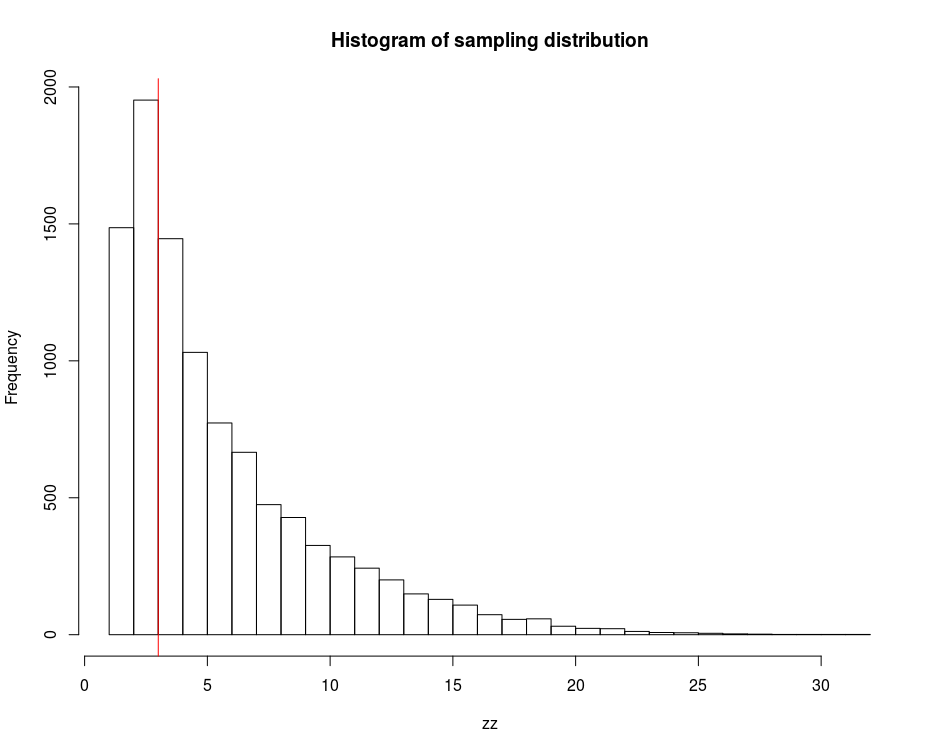
\includegraphics[width=\textwidth]{images/chapter3/connected_components/Rplot_ukbbed.png}
    \caption{Histogram of resampling of size of largest connected component n=58 in PSP UKBB Ed. 34.8\% less than or equal to 3. code \url{source('~/RProjects/chapter3/R/mouse_ltp/test_ukbbed_connected_component.R')}}
    \label{fig:my_label}
\end{figure}

 \subsubsection{Largest connected component and murine LTP}

Calculated the alrgest connect component induced by murine terms. 255 genes (should be 258 redo just need the more up to date data) are found in MP0002207 - abnormal long term potentiation. 140 of these are in the PSP. The largest connected component was 75 genes (140 nodes 125 edges in induced subgraph) 60 components largest 75. 

Resampling random samples of size 10000, 1 tailed t 0.0025

max 85.See figure~\ref{fig:histogram mouse ltp}

\begin{figure}
    \centering
    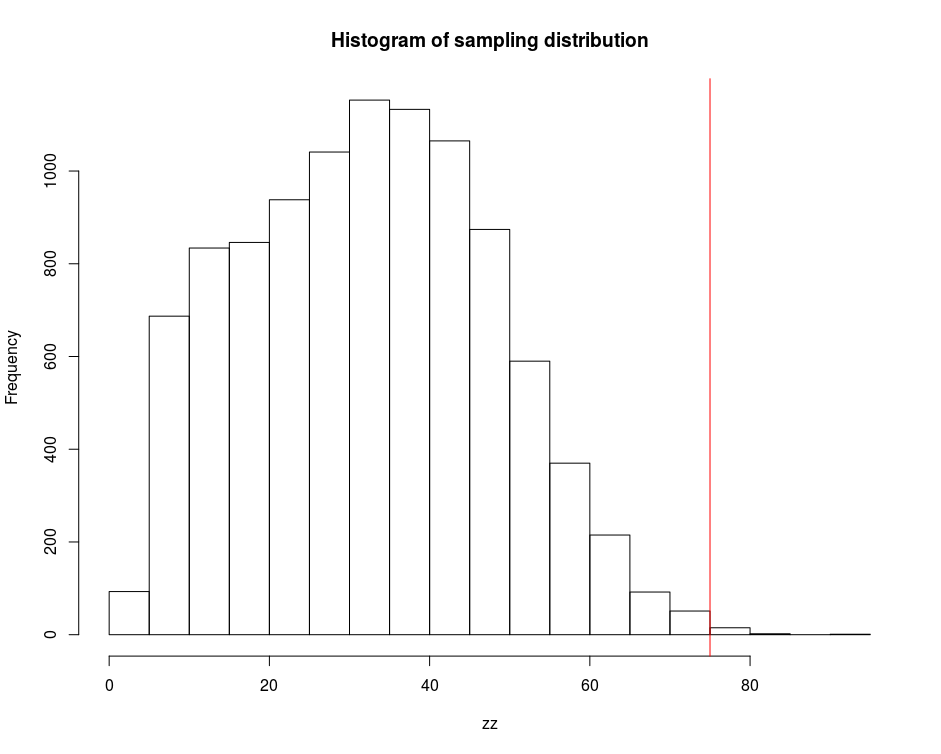
\includegraphics[width=\textwidth]{images/chapter3/connected_components/Rplot_mouse_abnormal_ltp_histogram_MP0002207.png}
    \caption{Histogram of resampling of size of largest connected component n=140 in PSP. Red line is size of mouse abnormal LTP 140 nodes in PSP. Largest component 75 Code\url{ source('~/RProjects/chapter3/R/mouse_ltp/test_murineLTP_connected_component.R')}}
    \label{fig:histogram mouse ltp}
\end{figure}
 
 \clearpage
 
 

\section{Characterisation of central genes}

To investigate whether central genes share common properties I carried out gene ontology enrichment of the top and bottom 10\% of genes for each centrality measures. The most central genes shared a number of common features regardless of the centrality measure. The top ten high degree nodes in terms of degree are shown for the purpose of illustration showing biological process table~\ref{tab:ToppGENE GO: Biological Process. 90 centile cwpsp.txtp = p value; q FDR B H = q adjusted significance level False Discovery Rate using Benjamini and Hochberg adjustment; n= n genes annotated in test group; n PSP= n genes annotated in PSP. n significant in category 1584} , cellular component table~\ref{tab:ToppGENE GO: Cellular Component. 90 centile cwpsp.txtp = p value; q FDR B H = q adjusted significance level False Discovery Rate using Benjamini and Hochberg adjustment; n= n genes annotated in test group; n PSP= n genes annotated in PSP. n significant in category 159} and molecular function (table~\ref{tab:ToppGENE GO: Cellular Component. 90 centile cwpsp.txtp = p value; q FDR B H = q adjusted significance level False Discovery Rate using Benjamini and Hochberg adjustment; n= n genes annotated in test group; n PSP= n genes annotated in PSP. n significant in category 159}). 

Biological process table~\ref{tab:ToppGENE GO: Biological Process. 90 centile cwpsp.txtp = p value; q FDR B H = q adjusted significance level False Discovery Rate using Benjamini and Hochberg adjustment; n= n genes annotated in test group; n PSP= n genes annotated in PSP. n significant in category 1584} shows enrichment for terms related to the cell cycle with low FDR values. Mplecular function terms include a number related to RNA binding and transcription table~\ref{tab:ToppGENE GO: Molecular Function. 90 centile cwpsp.txtp = p value; q FDR B H = q adjusted significance level False Discovery Rate using Benjamini and Hochberg adjustment; n= n genes annotated in test group; n PSP= n genes annotated in PSP. n significant in category 186}. Cellular component table~\ref{tab:ToppGENE GO: Cellular Component. 90 centile cwpsp.txtp = p value; q FDR B H = q adjusted significance level False Discovery Rate using Benjamini and Hochberg adjustment; n= n genes annotated in test group; n PSP= n genes annotated in PSP. n significant in category 159} shows enrichment for focal adhesion and cell junction terms, ribonucleoprotein and cytoskeletal fibre. 

These functions tend to be common across all centrality measures although there are some differences. Eigenvector centrality results in particularly strong enrichment for RNA binding as does eigenvector centrality and kcoreness. Transitivity shows far less enrichment than the other centrality terms reflecting its weaker correlation. It is interesting to note however that it selects a large proportion of the genes involved in mitochondrial translation and ribosomal function. 


Gene ontology enrichment has been carried out using the toppgene package and the PSP as a background set. These are therefore sets of genes that differ from the background enrichment of the PSP. Given that fact it is remarkable how many terms are enriched even after correcting for multiple comparisons (186 for example in the top 10\% of degree for molecular function table~\ref{tab:ToppGENE GO: Molecular Function. 90 centile cwpsp.txtp = p value; q FDR B H = q adjusted significance level False Discovery Rate using Benjamini and Hochberg adjustment; n= n genes annotated in test group; n PSP= n genes annotated in PSP. n significant in category 186}) and 1548 in Biological Process table~\ref{tab:ToppGENE GO: Biological Process. 90 centile cwpsp.txtp = p value; q FDR B H = q adjusted significance level False Discovery Rate using Benjamini and Hochberg adjustment; n= n genes annotated in test group; n PSP= n genes annotated in PSP. n significant in category 1584}.

By contrast fewer terms are enriched in low centrality gene sets for degree only two terms in cellular component were enriched (table~\ref{tab:ToppGENE GO: Cellular Component. 10 centile cwpsp.txtp = p value; q FDR B H = q adjusted significance level False Discovery Rate using Benjamini and Hochberg adjustment; n= n genes annotated in test group; n PSP= n genes annotated in PSP}). In part this is due to the fact that the distribution of centrality functions such as degree, betweenness and eigenvector centrality is right skewed. Closeness which is bounded in the region 0-1 and the most approximate to normally distributed provides more enrichment and these are genes one would expect on the periphery of the network and the synapse, those of the receptors themselves, intrinsic components of the plasma membrance and components of the extra cellular matrix. Kcoreness which has a relatively uniform distribution over a small range also has greater enrichment of low centrality terms.  (table~\ref{tab:ToppGENE Pathway. kco 10 centile cwpsp.txtp = p value; q FDR B H = q adjusted significance level False Discovery Rate using Benjamini and Hochberg adjustment; n= n genes annotated in test group; n PSP= n genes annotated in PSP. n significant in category 8}).

The overlap between different centrality measures ontology enrichment is shown in section~\ref{sec: ontology overlap} where the Jaccard index of the relationship between terms is shown


\begin{table}[ht]
\centering
\begin{adjustbox}{width=\textwidth}
\setlength{\extrarowheight}{2pt}

\begin{tabular}{@{}clllcl@{}}
  \toprule
ID & Molecular Function & $n$ & $n$ PSP & $p$ & $q$ FDR B H \\ 
  \midrule
GO:0031625 & ubiquitin protein ligase binding & 51 & 117 & $8.81 \times 10^{-22}$ & $9.12 \times 10^{-19}$ \\ 
  GO:0044389 & ubiquitin-like protein ligase binding & 52 & 123 & $1.88 \times 10^{-21}$ & $9.74 \times 10^{-19}$ \\ 
  GO:0008134 & transcription factor binding & 58 & 156 & $1.53 \times 10^{-20}$ & $5.26 \times 10^{-18}$ \\ 
  GO:0019904 & protein domain specific binding & 87 & 329 & $3.13 \times 10^{-19}$ & $8.11 \times 10^{-17}$ \\ 
  GO:0003723 & RNA binding & 120 & 554 & $5.07 \times 10^{-19}$ & $1.05 \times 10^{-16}$ \\ 
  GO:0044877 & protein-containing complex binding & 111 & 513 & $2.27 \times 10^{-17}$ & $3.91 \times 10^{-15}$ \\ 
  GO:0003720 & telomerase activity & 21 & 30 & $5.04 \times 10^{-15}$ & $7.00 \times 10^{-13}$ \\ 
  GO:0003964 & RNA-directed DNA polymerase activity & 22 & 33 & $5.41 \times 10^{-15}$ & $7.00 \times 10^{-13}$ \\ 
  GO:0034061 & DNA polymerase activity & 23 & 37 & $1.23 \times 10^{-14}$ & $1.41 \times 10^{-12}$ \\ 
  GO:0019900 & kinase binding & 78 & 325 & $1.50 \times 10^{-14}$ & $1.55 \times 10^{-12}$ \\ 
   \bottomrule
\end{tabular}
\end{adjustbox}
\caption[Gene ontology Molecular Function enrichment of genes above 90th centile of degree distribution]{\textbf{High degree genes. Molecular function - Gene ontology enrichment analysis} using the ToppGene web client and all PSP genes as the background set.  Molecular Function tested gene set is 90th centile of degree distribution.  p value; q FDR B H = q adjusted significance level False Discovery Rate using Benjamini and Hochberg adjustment; $n$= $n$ genes annotated in test group; $n$ PSP= n genes annotated in PSP. $n$ ontology terms significantly (q FDR$>=0.05$) enriched for this centrality measure and ontology category (e.g. MF,CC,BP): 186} 
\label{tab:ToppGENE GO: Molecular Function. 90 centile cwpsp.txtp = p value; q FDR B H = q adjusted significance level False Discovery Rate using Benjamini and Hochberg adjustment; n= n genes annotated in test group; n PSP= n genes annotated in PSP. n significant in category 186}
\end{table}
\paragraph{Biological process}

Biological process table~\ref{tab:ToppGENE GO: Biological Process. 90 centile cwpsp.txtp = p value; q FDR B H = q adjusted significance level False Discovery Rate using Benjamini and Hochberg adjustment; n= n genes annotated in test group; n PSP= n genes annotated in PSP. n significant in category 1584} shows enrichment for terms related to the cell cycle with low FDR values. 
% latex table generated in R 3.6.3 by xtable 1.8-4 package
% Sun Oct  4 15:30:52 2020
\begin{table}[ht]
\centering
\begin{adjustbox}{width=\textwidth}
\setlength{\extrarowheight}{2pt}
\begin{tabular}{@{}clllcl@{}}
  \toprule
  ID & Biological Process & $n$ & $n$ PSP & $p$ & $q$ FDR B H \\ 

  \midrule
GO:0007049 & cell cycle & 139 & 489 & $1.98 \times 10^{-36}$ & $1.25 \times 10^{-32}$ \\ 
  GO:0022402 & cell cycle process & 119 & 414 & $7.10 \times 10^{-31}$ & $2.25 \times 10^{-27}$ \\ 
  GO:0000280 & nuclear division & 101 & 319 & $1.43 \times 10^{-29}$ & $3.02 \times 10^{-26}$ \\ 
  GO:0048285 & organelle fission & 103 & 337 & $9.65 \times 10^{-29}$ & $1.53 \times 10^{-25}$ \\ 
  GO:0000278 & mitotic cell cycle & 95 & 296 & $3.44 \times 10^{-28}$ & $3.10 \times 10^{-25}$ \\ 
  GO:0140014 & mitotic nuclear division & 95 & 296 & $3.44 \times 10^{-28}$ & $3.10 \times 10^{-25}$ \\ 
  GO:1903047 & mitotic cell cycle process & 95 & 296 & $3.44 \times 10^{-28}$ & $3.10 \times 10^{-25}$ \\ 
  GO:0044403 & symbiotic process & 106 & 364 & $1.23 \times 10^{-27}$ & $9.33 \times 10^{-25}$ \\ 
  GO:0051726 & regulation of cell cycle & 100 & 329 & $1.33 \times 10^{-27}$ & $9.33 \times 10^{-25}$ \\ 
  GO:0044419 & interspecies interaction between organisms & 106 & 368 & $3.48 \times 10^{-27}$ & $2.20 \times 10^{-24}$ \\ 
   \bottomrule
\end{tabular}
\end{adjustbox}
\caption[Gene ontology enrichment Biological Process of genes above 90th centile of degree distribution]{\textbf{High degree genes. Biological Process - Gene ontology enrichment analysis} using the ToppGene web client and all PSP genes as the background set.  Biological process tested gene set is 90th centile of degree distribution.  p value; q FDR B H = q adjusted significance level False Discovery Rate using Benjamini and Hochberg adjustment; $n$= $n$ genes annotated in test group; $n$ PSP= n genes annotated in PSP. $n$ ontology terms significantly (q FDR$>=0.05$) enriched for this centrality measure and ontology category (e.g. MF,CC,BP): 1584} 

\label{tab:ToppGENE GO: Biological Process. 90 centile cwpsp.txtp = p value; q FDR B H = q adjusted significance level False Discovery Rate using Benjamini and Hochberg adjustment; n= n genes annotated in test group; n PSP= n genes annotated in PSP. n significant in category 1584}
\end{table}


\paragraph{Cellular component}


Cellular component table~\ref{tab:ToppGENE GO: Cellular Component. 90 centile cwpsp.txtp = p value; q FDR B H = q adjusted significance level False Discovery Rate using Benjamini and Hochberg adjustment; n= n genes annotated in test group; n PSP= n genes annotated in PSP. n significant in category 159} shows enrichment for focal adhesion and cell junction terms, ribonucleoprotein and cytoskeletal fibre. 

% latex table generated in R 3.6.3 by xtable 1.8-4 package
% Sun Oct  4 15:33:48 2020
\begin{table}[ht]
\centering
\begin{adjustbox}{width=\textwidth}
\setlength{\extrarowheight}{2pt}
\begin{tabular}{@{}clllcl@{}}
  \toprule
  ID & Cellular Component & $n$ & $n$ PSP & $p$ & $q$ FDR B H \\ 

  \midrule

GO:1990904 & ribonucleoprotein complex & 81 & 303 & $2.75 \times 10^{-18}$ & $2.36 \times 10^{-15}$ \\ 
  GO:0015630 & microtubule cytoskeleton & 102 & 447 & $1.01 \times 10^{-17}$ & $4.33 \times 10^{-15}$ \\ 
  GO:0036464 & cytoplasmic ribonucleoprotein granule & 33 & 74 & $8.92 \times 10^{-15}$ & $2.55 \times 10^{-12}$ \\ 
  GO:0035770 & ribonucleoprotein granule & 33 & 78 & $5.84 \times 10^{-14}$ & $1.25 \times 10^{-11}$ \\ 
  GO:1902494 & catalytic complex & 86 & 392 & $1.07 \times 10^{-13}$ & $1.84 \times 10^{-11}$ \\ 
  GO:0030055 & cell-substrate junction & 62 & 244 & $7.12 \times 10^{-13}$ & $1.02 \times 10^{-10}$ \\ 
  GO:0005925 & focal adhesion & 61 & 239 & $9.13 \times 10^{-13}$ & $1.12 \times 10^{-10}$ \\ 
  GO:0000974 & Prp19 complex & 19 & 31 & $3.66 \times 10^{-12}$ & $3.92 \times 10^{-10}$ \\ 
  GO:0099513 & polymeric cytoskeletal fiber & 95 & 482 & $4.16 \times 10^{-12}$ & $3.96 \times 10^{-10}$ \\ 
  GO:0005815 & microtubule organizing center & 60 & 246 & $1.21 \times 10^{-11}$ & $1.04 \times 10^{-9}$ \\ 
   \hline
\end{tabular}
\end{adjustbox}
\caption[Gene ontology enrichment Cellular Component of genes above 90th centile of degree distribution]{\textbf{High degree genes. Cellular Component - Gene ontology enrichment analysis} using the ToppGene web client and all PSP genes as the background set.  Biological process tested gene set is 90th centile of degree distribution.  p value; q FDR B H = q adjusted significance level False Discovery Rate using Benjamini and Hochberg adjustment; $n$= $n$ genes annotated in test group; $n$ PSP= n genes annotated in PSP. $n$ ontology terms significantly (q FDR$>=0.05$) enriched for this centrality measure and ontology category (e.g. MF,CC,BP): 159} 
\label{tab:ToppGENE GO: Cellular Component. 90 centile cwpsp.txtp = p value; q FDR B H = q adjusted significance level False Discovery Rate using Benjamini and Hochberg adjustment; n= n genes annotated in test group; n PSP= n genes annotated in PSP. n significant in category 159}
\end{table}



across all of theGene ontology enrichment of the most central vertices reveals that they share a number of common properties across different





\subsection{Moved from other sections}
\paragraph{Results GO enrichment Closeness}
More normally distributed.
High closeness RNA binding, severe murine phenotype, cellular component cell adhesion
Ca and neurodegenerative

Low closeness centrality transporter activity, seizures in human phenotype, receptor activation, disease top five all epilepsies. 

\subsection{Degree}
High degree nodes are enriched for terms associated with RNA binding, cell cycle and ubiquitin binding. This would be consistent with these high degree nodes being involved in central cellular processes\footnote{\url{source('~/RProjects/chapter3/R/sig_magma_genes/central_genes_ToppGene/degree/5_0_clip_centrality_degree_high_mf_n_10.R')}}.

\paragraph{Molecular function}
Molecular function table~\ref{tab:ToppGENE GO: Molecular Function. 90 centile cwpsp.txtp = p value; q FDR B H = q adjusted significance level False Discovery Rate using Benjamini and Hochberg adjustment; n= n genes annotated in test group; n PSP= n genes annotated in PSP. n significant in category 186} shows enrichment for ubiquitin protein ligase, RNA binding and transcription factor binding. The q values are not as significant as those for kcoreness and eigenvector centrality.

% latex table generated in R 3.6.3 by xtable 1.8-4 package
% Sun Oct  4 15:28:01 2020



\subsubsection{Low degree}
The only gene ontology class enriched was cellular component (table~\ref{tab:ToppGENE GO: Cellular Component. 10 centile cwpsp.txtp = p value; q FDR B H = q adjusted significance level False Discovery Rate using Benjamini and Hochberg adjustment; n= n genes annotated in test group; n PSP= n genes annotated in PSP}) but the enriched terms are common in other low vaules of centrality measures in that it is enriched for components of the plasma membrane. Pathway enrichment shows enrichment of the extracellular matrix and ECM proteins which is found with other low centrality measure genes in PANTHER. The results for high and low degree genes appear qualitatively different even compared to other post synaptic protein genes (ie cell cycle processes verus ECM). The network architecture seems to be related to function but is it related to the phenotype?



% latex table generated in R 3.6.3 by xtable 1.8-4 package 
% Sat Oct  3 17:17:17 2020
\begin{table}[ht]
\centering

\begin{adjustbox}{width=\textwidth}
\setlength{\extrarowheight}{2pt}
\begin{tabular}{@{}clllcl@{}}
  \toprule
  ID & Cellular Component &$p$ & $q$ FDR B H  & $n$ & $n$ PSP  \\ 
  \midrule
GO:0031226 & intrinsic component of plasma membrane & $1.564 \times 10^{-5}$ & $7.462 \times 10^{-3}$ & 51 & 331 \\ 
  GO:0005887 & integral component of plasma membrane & $4.228 \times 10^{-5}$ & $1.008 \times 10^{-2}$ & 47 & 307 \\ 
   \bottomrule
\end{tabular}
\end{adjustbox}
\caption{ToppGene GO: Cellular Component. 10 centile cwpsp.txtp = p value; q FDR B H = q adjusted significance level False Discovery Rate using Benjamini and Hochberg adjustment; n= n genes annotated in test group; n PSP= n genes annotated in PSP. \textcolor{red}{columns in different order from above ? change}} 
\label{tab:ToppGENE GO: Cellular Component. 10 centile cwpsp.txtp = p value; q FDR B H = q adjusted significance level False Discovery Rate using Benjamini and Hochberg adjustment; n= n genes annotated in test group; n PSP= n genes annotated in PSP}
\end{table}


Pathway table~\ref{tab:ToppGENE Pathway. 10 centile cwpsp.txtp = p value; q FDR B H = q adjusted significance level False Discovery Rate using Benjamini and Hochberg adjustment; n= n genes annotated in test group; n PSP= n genes annotated in PSP} 

% latex table generated in R 3.6.3 by xtable 1.8-4 package
% Sat Oct  3 17:21:16 2020
\begin{table}[ht]
\centering
\begin{adjustbox}{width=\textwidth}
\setlength{\extrarowheight}{2pt}
\begin{tabular}{@{}clllcl@{}}

  \toprule
ID & Pathway & p & q FDR B H & n & n PSP \\ 
  \midrule
M5889 & \makecell{Ensemble of genes encoding extracellular matrix and\\ extracellular matrix-associated proteins}  & $5.689 \times 10^{-6}$ & $5.831 \times 10^{-3}$ & 19 & 91 \\ 
  1269590 & Adenylate cyclase activating pathway & $9.603 \times 10^{-5}$ & $4.798 \times 10^{-2}$ & 4 & 5 \\ 
  1269923 &\makecell{ Transport of glucose and other sugars, bile salts and organic acids,\\ metal ions and amine compounds} & $2.551 \times 10^{-4}$ & $4.798 \times 10^{-2}$ & 5 & 10 \\ 
  1272485 & Aldosterone synthesis and secretion & $2.896 \times 10^{-4}$ & $4.798 \times 10^{-2}$ & 9 & 34 \\ 
  1269930 & Metal ion SLC transporters & $3.277 \times 10^{-4}$ & $4.798 \times 10^{-2}$ & 3 & 3 \\ 
   \bottomrule
\end{tabular}
\end{adjustbox}
\caption{ToppGene Pathway. 10 centile cwpsp.txtp = p value; q FDR B H = q adjusted significance level False Discovery Rate using Benjamini and Hochberg adjustment; n= n genes annotated in test group; n PSP= n genes annotated in PSP} 
\tiny\url{source('~/RProjects/chapter3/R/sig_magma_genes/central_genes_toppgene/betweenness/5_0_clip_centrality_bet_hig_mf.R')}

\label{tab:ToppGENE Pathway. 10 centile cwpsp.txtp = p value; q FDR B H = q adjusted significance level False Discovery Rate using Benjamini and Hochberg adjustment; n= n genes annotated in test group; n PSP= n genes annotated in PSP}
\end{table}




\clearpage

 
\subsubsection{The PSP is over-represented in essential genes}
\label{sec:results over representation PSP in DEG genes}
Genes in the post synaptic proteome are over-represented amongst essential genes as defined in the DEG. Table~\ref{tab:DEG any appearance contingency table PSP vs not PSP} shows the contingency table for genes being in the PSP or not and appearing more than once in the PSP. The PSP had 2,328 genes that appeared at least once in the DEG (    $n$ genes in PSP = 3457 ; 67.3\%) compared with 6,664 non PSP genes (41.7\% of 15,970 non synaptic genes appearing in NCBI 37). Although synaptic genes are more likely to be essential than non synaptic genes, central synaptic genes are even more likely to be essential (from the DEG data). 


\begin{table}
\centering
\begin{tabular}{cccc}
\toprule
& \multicolumn{2}{c}{Essential} & \\
\cmidrule{2-3}
    PSP & Essential &  Non-Essential & Total by PSP\vspace{1mm} \\
\midrule 
PSP      &   2,328     &     1,129 & 3,457\vspace{1mm}\\
not PSP    &  6,664      &    9,306  & 15,970\vspace{1mm}\\
\midrule
 Total by essential & 8,992 & 10,435 &  19,427\\ 

 
\bottomrule
\end{tabular}
\caption{Contingency table showing essential genes where essentialness is appearing once in the Database of Essential Genes (DEG). Total genes (19427).  Fisher's exact test p$<2.2\times10^{-16}$. OR 2.88 95\% CI 2.66 3.12; OR 2.92. Results checked Mar}
\tiny\url{source('~/RProjects/db_essential_genes/R/get_essential_genes/db_2020/findforfive/get_db_essential_greater_five_results_xtable_transpose.R')}  
\label{tab:DEG any appearance contingency table PSP vs not PSP}
\end{table}




Using the more strict deginitiion of essentialness (that aims to correspond with estimates of 10\% of human genes) $n$ = 728 (21.1\%) of PSP genes appear in five or more experiments in the DEG. By contrast the figure for non PSP genes is $n$=1,450 (9.99\%) (table~\ref{tab:DEG five or more appearances in contingency table PSP vs not PSP}). 

   \begin{table}
\centering
\begin{tabular}{cccc}
\toprule
& \multicolumn{2}{c}{Essential} & \\
\cmidrule{2-3}
    PSP & Essential &  Non-Essential & Total by PSP\vspace{1mm} \\
\midrule 
PSP      &   728     &     2,729 & 3,457\vspace{1mm}\\
not PSP    &  1,450      &    14,520  & 15,970\vspace{1mm}\\
\midrule
 Total by essential & 2,178 & 10,435 &  19,427\\ 

 
\bottomrule
\end{tabular}
\caption{Contingency table showing essential genes where essentialness is appearing five or more times  in the Database of Essential Genes (DEG). Total genes (19427).  Fisher's exact test p$<2.2\times10^{-16}$. OR 2.67 ;95\% CI 2.42 - 2.95; OR 2.67. Results checked Mar}
\tiny\url{source('~/RProjects/db_essential_genes/R/get_essential_genes/db_2020/findforfive/get_db_essential_greater_five_results_xtable_transpose.R')}  
\label{tab:DEG five or more appearances in contingency table PSP vs not PSP}
\end{table}
    
Fisher's exact test  for over representation in synaptic genes for any appearance in the DEG (OR 2.879; 2.663-3.115) and more than five appearances in the DEG (OR 2.671; 2.418-2.949) are shown in table (table~\ref{tab:Fishers exact results DEG}).

% latex table generated in R 3.6.3 by xtable 1.8-4 package
% Thu Mar 18 14:19:31 2021
\begin{table}[ht]
\centering
\begin{tabular}{lllll}

  \toprule
Study & Odds ratio & 95\% CI Lower & 95\%CI Upper & p \\ 
  \midrule
Any DEG vs none & 2.879 & 2.663 & 3.115 & $1.968 \times 10^{-166}$\vspace{1mm} \\ 
  Greater than 5 DEG v none & 2.671 & 2.418 & 2.949 & $6.162 \times 10^{-79}$\vspace{1mm} \\ 
   \bottomrule
\end{tabular}
\caption{Fishers exact test for over representation of synaptic genes in DEG (database of essential genes). First is any appearance in DEG vs genes not in DEG. Second is those in five or more (see methods)Confidence intervals and significance for over representation of PSP proteins in Database of Essential Genes (DEG)}
\tiny\textsuperscript{source=} \url{source('~/RProjects/db_essential_genes/R/get_essential_genes/db_2020/findforfive/get_db_essential_greater_five_results_xtable_transpose.R')}
\label{tab:Fishers exact results DEG}
\end{table}

Synaptic genes are significantly more likely to be essential according to the DEG.

\subsubsection{Feb redo: Centrality and DEG genes}


   

The values of the centrality measures seem to be highest in genes that are in 5 or more studies in the DEG, next highest in those appearing in more than one and less than five and lowest in those that do not appear in the DEG as can be seen in the boxplots in figure~\ref{fig:boxplot_three_groups_DEG_multiplot1}. Degree, eigenvector centrality and betweenness centrality are shown in a log10 scale (see figure~\ref{fig:boxplot_three_groups_DEG_logdegree1} for a larger image of the degree boxplot). The plot in figure~\ref{fig:boxplot_log degree essential genes} again shows the relationship of degree centrality to essentialness but in this case showing only genes in the PSP not in the list of essential genes and those in the list of essential genes. The difference in the median values is clear even in the logarithmic plot. 

\textcolor{red}{Start of with difference in greater than 5 compared to one or more compared to none and then at end do linear relationship}
The correlation between node centrality and the number of studies in the DEG that the gene appears in is shown in table~\ref{tab:Correlation centrality and num studies DEG}. There appears to be a correlation between the number of studies in which a gene is found to be central and its centrality measure (Spearman's $\rho$). The relationship is strongest for eigenvector centrality ($\rho=0.398$) and weakest for transitivity $\rho=0.207$. The betweenness centrality is the second smallest (transitivity often has weak effects compared to other centrality measures) $\rho=0.243$.




% above from https://tex.stackexchange.com/questions/84527/include-centered-full-page-figure-with-no-margins

\begin{figure}[p]
    \vspace*{-2cm}
    \makebox[\linewidth]{
        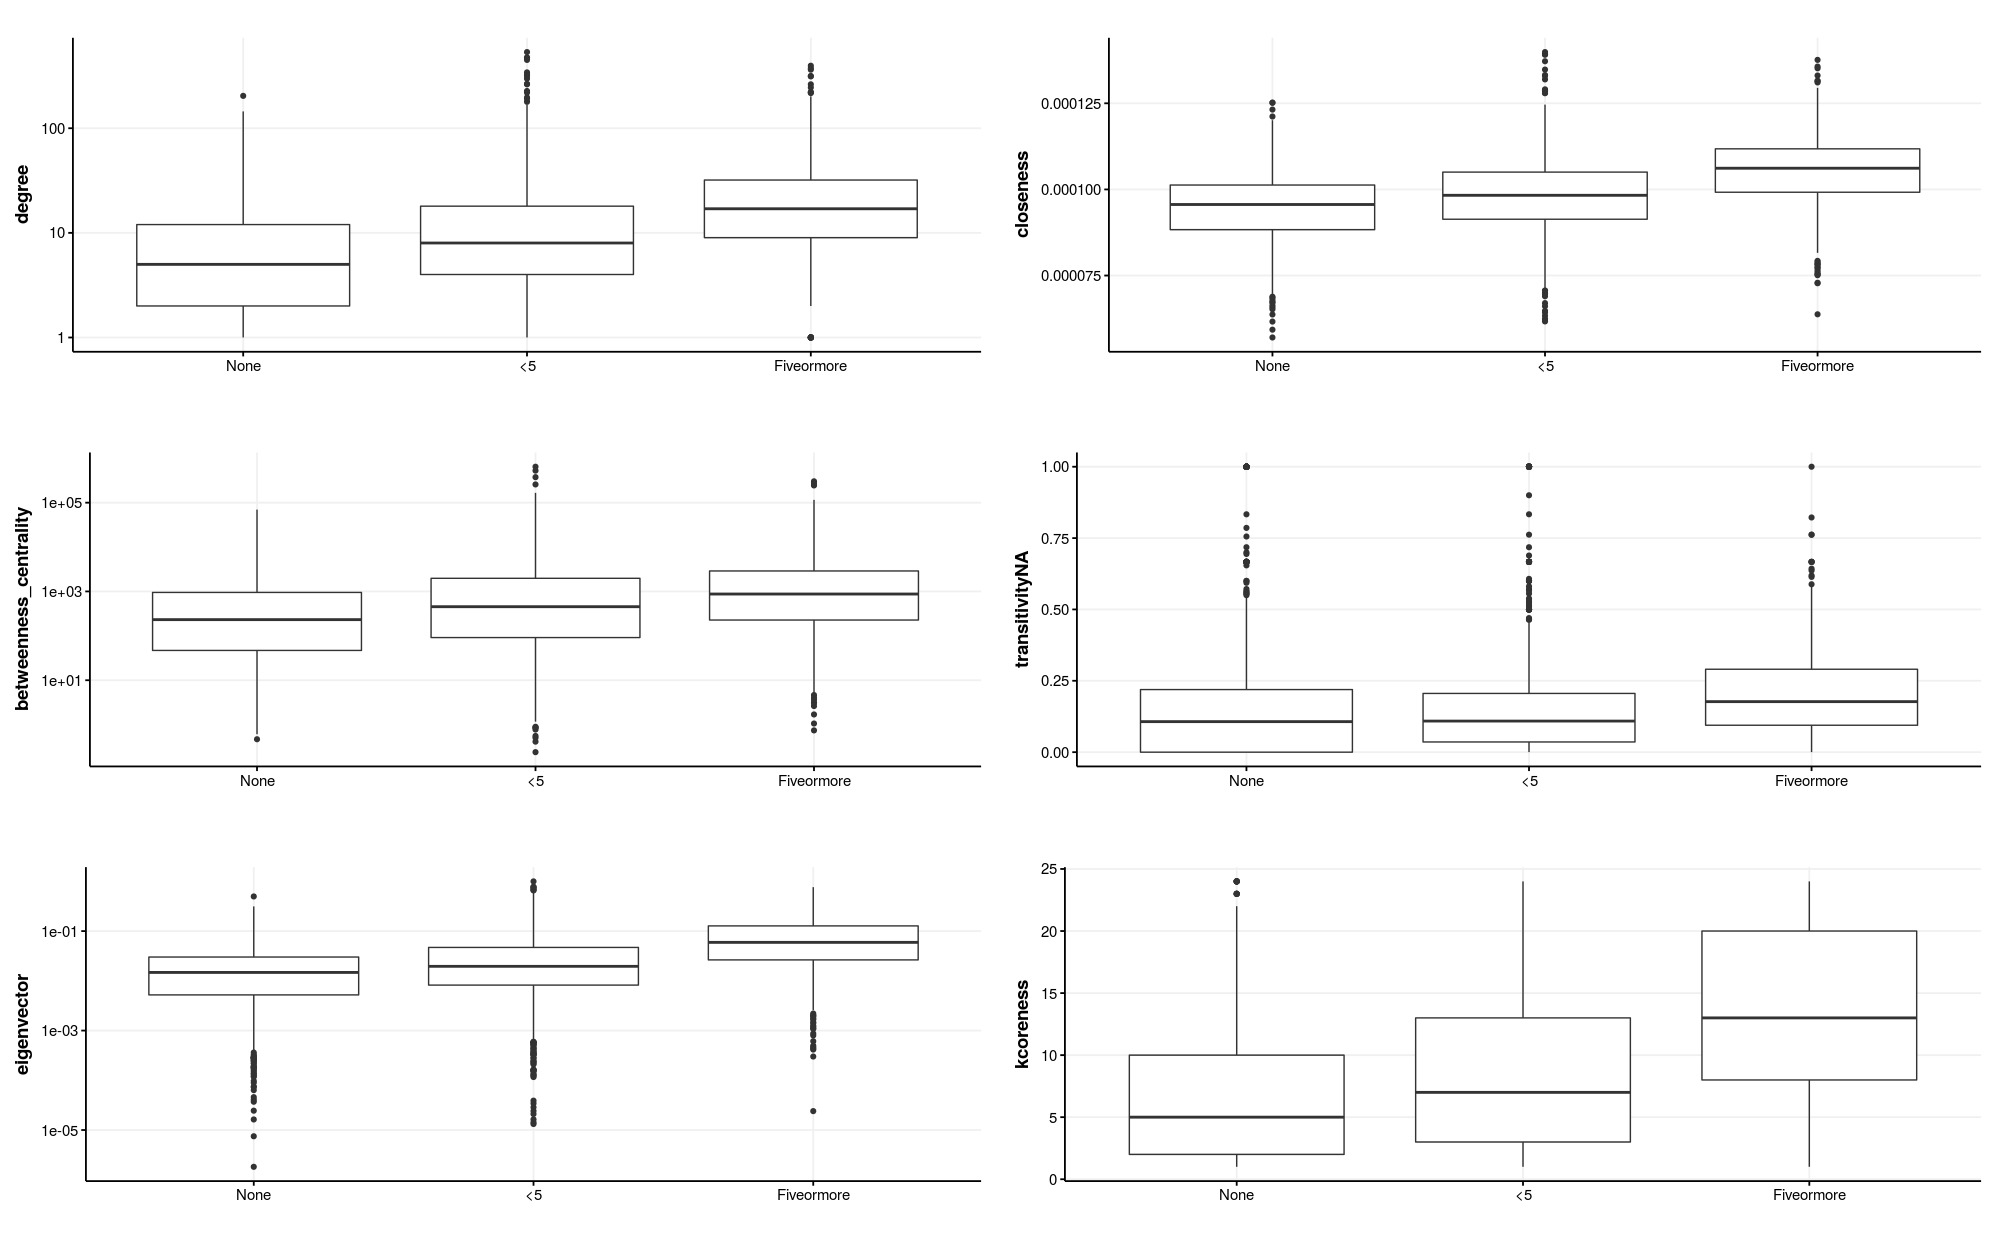
\includegraphics[width=1.3\linewidth, height=20cm]{images/chapter3/ggplot2/db_essential_genes/theme/Rplot_multiplot_with_theme_simple.png}}
    \caption{Multiplot of boxplot of centralities and DEG. On the x axis categories are non essential, Up to 5 appearances in DEG, 5 or more appearances in DEG }
    \tiny\url{ source('~/RProjects/db_essential_genes/R/get_essential_genes/db_2020/theme/get_db_essential_threecategoriesboxplot_multiplot_no_x_lab_essential_centrality_theme.R')}
\end{figure}

% latex table generated in R 3.6.3 by xtable 1.8-4 package
% Fri Feb 26 14:53:35 2021
\begin{table}[ht]
\centering
\begin{tabular}{lcrc}
  \toprule
Centrality Measure & S & rho & p \\ 
  \midrule
 Degree  & $1.401 \times 10^{9}$ & 0.334 & $1.265 \times 10^{-61}$ \\ 
 Eigenvector   & $1.266 \times 10^{9}$ & 0.398 & $3.479 \times 10^{-89}$ \\ 
 Betweenness centrality   & $1.591 \times 10^{9}$ & 0.243 & $9.620 \times 10^{-33}$ \\ 
   Closeness   & $1.341 \times 10^{9}$ & 0.362 & $4.825 \times 10^{-73}$ \\ 
  TransitivityNA   & $1.378 \times 10^{9}$ & 0.207 & $1.233 \times 10^{-22}$ \\ 
  kcoreness   & $1.336 \times 10^{9}$ & 0.365 & $4.081 \times 10^{-74}$ \\ 
   \bottomrule
\end{tabular}
\caption{Correlation of centrality measures and number of studies (max 20) found in DEG. Correlation type spearman.}
\tiny\url{source('~/RProjects/db_essential_genes/R/get_essential_genes/db_2020/findforfive/clean_up/get_db_essential_five_or_more_ttests_essential_centrality_correlation_count_centrality.R')}
\label{tab:Correlation centrality and num studies DEG}
\end{table}
\subsubsection{Assortativity and essential genes}
\label{sec:Assortativity and essential genes}
Latest 

assortativity nominal 0.0355
code\url{source('~/RProjects/db_essential_genes/R/get_essential_genes/assortativity_essential_genes.R')}

\subsubsection{Essential gene conclusion}
PSP genes are more likely to be essential. Essential genes are of higher degree than non essential genes. There is a very weak assortativity for essential genes. 

\todo{DONE Degree etc for essential genes}
\todo{Essential genes enrichment vs non essential PSP add to community detection section}
\todo{Essential gene count for significant genes vs psp genes}



\section{Probability of loss of function intolerance (pLI)}
\label{sec: results pLI}


The probability of loss of function intolerance is associated with measures of vertex centrality in the post synaptic proteome graph. The correlation is greatest for degree ($\rho=0.230$) and lowest for transitivity ($\rho=0.086$). Betweenness and eigenvector centrality have similar correlation to loss of function intolerance as degree (see table \ref{tab:correlation pli vertex statistics mar})

\subsection{Distribution of pLI}
\label{sec:results distribution of pli}
The distribution of the probability of loss of function intolerance based on Gnomad v2.1.1 (section~\ref{sec:methods exac and gnomad} is shown as a stacked histogram in  figure~\ref{fig:hist_pliPSP_theme} and as a density plot in figure~\ref{fig:densityPLI_theme}. Both plots show a bimodal distribution of probability of loss of function intolerance with the probability mass centred at extreme high and low values and then a low level of probability mass between these extremes. The PSP genes (green in figure~\ref{fig:hist_pliPSP_theme} and the yellow-brown line in figure~\ref{fig:densityPLI_theme}) have a roughly symmetrical distribution with similar density at high and low probability of loss of function intolerance while the peak at low levels of probability of loss of function intolerance is much higher in the non PSP genes. This reflects a greater evolutionary constraint on the PSP genes and is consistent with the findings using the database of essential genes (section~\ref{sec:results over representation PSP in DEG genes}) but with the additional benefit of a \textit{measure} of selection pressure. 


The median pLI is higher for the PSP genes than non PSP (0.246 vs 0.001). The median PSP is greater than the third quartile of non PSP genes (table~\ref{tab:Probability of loss of function intolerance in genes in PSP versus those not in PSP}) and it is clear that the means are significantly different (Wilcoxon rank sum test with continuity correction W=17,893,688 $p<2.2\times10^{-16}$) \footnote{\url{source('~/RProjects/db_essential_genes/R/gnomad/histogram_pli_psp/statistics/summary_pLI_PSP.R')}}.


\begin{figure}
    \centering
    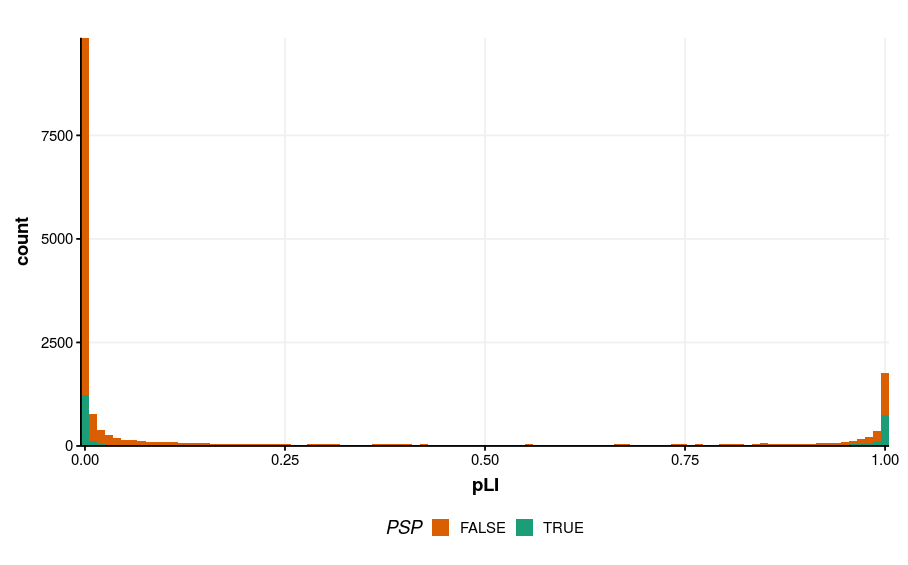
\includegraphics[width=\textwidth]{images/chapter3/ggplot2/gnomad/theme/Rplot_histogram_pLI_theme.png}
    \caption[Histogram of pLI comparing PSP and non PSP genes]{Stacked histogram showing the distribution of pLI in PSP and non PSP genes. The distribution is bimodal with most of the probability mass at extreme low and high values of pLI however the PSP genes have a more symmetrical distribution with a relatively higher peak in the high probability of loss of function intolerance range.}
    \tiny\url{source('~/RProjects/db_essential_genes/R/gnomad/histogram_pli_psp/theme/histogram_pli_theme.R')}
    
    \label{fig:hist_pliPSP_theme}
\end{figure}



\begin{figure}
    \centering
    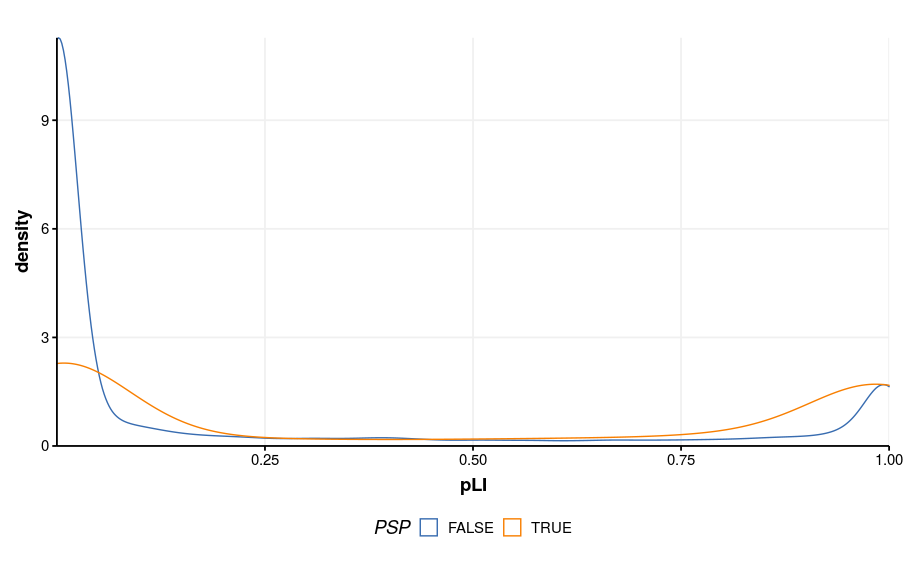
\includegraphics[width=\textwidth]{images/chapter3/ggplot2/gnomad/theme/Rplot_density_Mar_gnomad_theme.png}
    \caption[Density plot pLI for PSP and non PSP genes]{Density plot of pLI for PSP and non PSP. The distribution of probability loss intolerance is bimodal for both the PSP and non PSP genes with peaks at extreme low and high PSP values. The plot is more symmetrical for the PSP genes which shows a similar density of very high and very low probability of loss intolerance (pLI) values compared with the non PSP genes which, if they have extreme values are more likely to have low pLI}
    \tiny\url{source('~/RProjects/db_essential_genes/R/gnomad/histogram_pli_psp/theme/density_pli_theme.R')}
    
    \label{fig:densityPLI_theme}
\end{figure}






% latex table generated in R 3.6.3 by xtable 1.8-4 package
% Sun Mar 28 17:46:00 2021
\begin{table}[ht]
\centering
\setlength{\extrarowheight}{2pt}
\begin{adjustbox}{width=\textwidth}
\begin{tabular}{lllllllllll}
  \toprule
 & mean & median & sd & IQR & Q1 & Q3 & min & max & $n$ \\ 
  \midrule
PSP & 0.45 & 0.246 & 0.45 & 0.99 & $3.118 \times 10^{-5}$ & 0.988 & $1.861 \times 10^{-164}$ & 1 & 3407  \\ 
  non PSP & 0.20 & 0.001 & 0.35 & 0.23 & $2.068 \times 10^{-8}$ & 0.231 & $8.222 \times 10^{-118}$ & 1 & 14972 \\ 
   \bottomrule
\end{tabular}
\end{adjustbox}
\caption[Summary statistics PSP versus non PSP genes pLI]{Probability of loss of function intolerance in genes in PSP versus those not in PSP. Wilcoxon rank sum test with continuity correction W=17893688, $p<2.2\times10^{-16}$. No missing values. Q1 = first quartile, Q3 = third quartile, sd = standard deviation, IQR = interquartile range} 
\tiny\url{source('~/RProjects/db_essential_genes/R/gnomad/histogram_pli_psp/statistics/summary_pLI_PSP.R')}
\label{tab:Probability of loss of function intolerance in genes in PSP versus those not in PSP}
\end{table}




\subsubsection{Assortativity and pLI}

\subsection{Distribution of pLI and intelligence}
\todo{Distribution of pLI and intelligence}



%pLI z Spearman
% latex table generated in R 3.6.3 by xtable 1.8-4 package
% Tue Mar 23 15:38:29 2021
\begin{table}[ht]
\centering
\setlength{\extrarowheight}{2pt}
\begin{tabular}{llll}
  \toprule
Sample & $S$ & rho & $p$ \\ 
  \midrule
Intelligence\textsubscript{Replication} & $8.41 \times 10^{11}$ & 0.031 & $3.542 \times 10^{-5}$ \\ 
  Education\textsubscript{Replication} & $7.95 \times 10^{11}$ & 0.046 & $2.054 \times 10^{-9}$ \\ 
  Intelligence\textsubscript{Discovery} & $8.18 \times 10^{11}$ & 0.057 & $8.756 \times 10^{-14}$ \\ 
  Education\textsubscript{Discovery} & $8.01 \times 10^{11}$ & 0.077 & $6.338 \times 10^{-24}$ \\ 
   \bottomrule
\end{tabular}
\caption{Correlation pLI and z score Spearman } 
\tiny\url{source('~/RProjects/chapter3/R/magma_gnomad/compare_Mar/0_load_magma_and_load_gnomad.R')}
\label{tab: Correlation pLI and z score Spearman}
\end{table}


\begin{table}[ht]
\centering
\setlength{\extrarowheight}{2pt}
\begin{tabular}{lllllll}
  \toprule
Sample & $t$ & df & low & high & $r$ & $p$ \\ 
  \midrule
Intelligence\textsubscript{Replication} & 7.526 & 17334 & 0.042 & 0.072 & 0.057 & $5.470 \times 10^{-14}$ \\ 
  Education\textsubscript{Replication} & 9.234 & 17098 & 0.056 & 0.085 & 0.070 & $2.893 \times 10^{-20}$ \\ 
  Intelligence\textsubscript{Discovery} & 10.043 & 17324 & 0.061 & 0.091 & 0.076 & $1.150 \times 10^{-23}$ \\ 
  Education\textsubscript{Discovery} & 14.230 & 17324 & 0.093 & 0.122 & 0.107 & $1.078 \times 10^{-45}$ \\ 
   \bottomrule
\end{tabular}
\caption{Correlation pLI and z score Pearson } 
\tiny\url{source('~/RProjects/chapter3/R/magma_gnomad/compare_Mar/0_load_magma_and_load_gnomad.R')}
\label{tab: Correlation pLI and z score Pearson}
\end{table}



There was a weak association between probability of loss of function intolerance and gene score in this case z score. In table \ref{tab: Correlation pLI and z score Spearman} there is a weak but significant correlation between $z$ score and probability of loss of function intolerance. Genes that were more likely to be significant in these samples were more likely to be loss of function intolerant. Table~\ref{tab: Correlation pLI and neg log10 Spearman} shows the correlation is shown with the negative log10 transform of the p value, again a significant gene has a low p values and hence high -log10(P) transform so this table is showing the same thing, more significant genes are more loss of function intolerant. As they are shown with Spearman's rank correlation $\rho$ is identical as they are in the same rank order. Results showing the difference in relationship between synaptic and non synaptic genes in these cohorts are shown in table ~\ref{tab: Correlation pLI and neg log10 SpearmanPSP, nonPSP and all}  \footnote{\url{source('~/RProjects/paper_xls_output/R/make_df_correlation_pLI_genescore.R')}} the relationship is stronger for synaptic genes than for non synaptic genes although the effect is small and synaptic genes as shown below have a higher probability of loss of function intolerance.



\paragraph{Mar Correlation PLI}
The Pearson correlation between pLI and gene z score is highest for Education\textsubscript{Discovery} (r=0.107) and lowest for Intelligence\textsubscript{Replication}(r=0.057) (table~\ref{tab: Correlation pLI and z score Pearson}). For a non parametric test of correlation (table~\ref{tab: Correlation pLI and z score Spearman} Education\textsubscript{Discovery} is most correlated ($\rho$=0.077).

Using the negative log 10 transform of the MAGMA p values the highest Pearson correlation was with Education\textsubscript{Discovery} r=0.095 (table~\ref{tab: Correlation pLI and neg log10 Pearson}). The Education\textsubscript{Discovery} sample shows the highest correlation between log10 p and pLI ($\rho$=0.077) (table~\ref{tab: Correlation pLI and neg log10 Spearman})


% pLI z Pearson
% latex table generated in R 3.6.3 by xtable 1.8-4 package
% Tue Mar 23 15:35:23 2021




% pLI log10 Pearson

% latex table generated in R 3.6.3 by xtable 1.8-4 package
% Tue Mar 23 15:41:18 2021
\begin{table}[ht]
\centering
\setlength{\extrarowheight}{2pt}
\begin{tabular}{lllllll}
  \toprule
Sample & $t$ & df & low & high & $r$ & $p$ \\ 
\midrule
Intelligence\textsubscript{Replication} & 8.161 & 17334 & 0.047 & 0.077 & 0.062 & $3.546 \times 10^{-16}$ \\ 
  Education\textsubscript{Replication} & 10.534 & 17098 & 0.065 & 0.095 & 0.080 & $7.214 \times 10^{-26}$ \\ 
  Intelligence\textsubscript{Discovery} & 9.735 & 17324 & 0.059 & 0.089 & 0.074 & $2.440 \times 10^{-22}$ \\ 
  Education\textsubscript{Discovery} & 12.544 & 17324 & 0.080 & 0.110 & 0.095 & $6.141 \times 10^{-36}$ \\ 
   \bottomrule
\end{tabular}
\caption{Correlation pLI and neg log10 Pearson } 
\tiny\url{source('~/RProjects/chapter3/R/magma_gnomad/compare_Mar/0_load_magma_and_load_gnomad.R')}
\label{tab: Correlation pLI and neg log10 Pearson}
\end{table}



% PLI log10 Spearman

% latex table generated in R 3.6.3 by xtable 1.8-4 package
% Tue Mar 23 15:42:11 2021
\begin{table}[ht]
\centering
\setlength{\extrarowheight}{2pt}
\begin{tabular}{llll}
  \toprule
Sample & $S$ & rho & $p$ \\ 
  \midrule
Intelligence\textsubscript{Replication} & $8.41 \times 10^{11}$ & 0.031 & $3.542 \times 10^{-5}$ \\ 
  Education\textsubscript{Replication} & $7.95 \times 10^{11}$ & 0.046 & $2.054 \times 10^{-9}$ \\ 
  Intelligence\textsubscript{Discovery} & $8.18 \times 10^{11}$ & 0.057 & $8.754 \times 10^{-14}$ \\ 
  Education\textsubscript{Discovery} & $8.01 \times 10^{11}$ & 0.077 & $6.340 \times 10^{-24}$ \\ 
   \bottomrule
\end{tabular}
\caption{Correlation pLI and neg log10 Spearman } 
\tiny\url{source('~/RProjects/chapter3/R/magma_gnomad/compare_Mar/0_load_magma_and_load_gnomad.R')}
\label{tab: Correlation pLI and neg log10 Spearman}
\end{table}




\paragraph{Subsets}


The correlation between pLI and zscore is shown for subsets of the PSP, non PSP and all genes (table~\ref{tab: Correlation pLI and neg log10 SpearmanPSP, nonPSP and all}). The highest correlation is again in the Education\textsubscript{Discovery} sample and correlation is highest in PSP gene although PSP genes do have higher average pLI (although this shouldn't affect their rank correlation with gene score). 

The correlation is also shown between pLI and the negative log 10 transform of the gene p value (table~\ref{tab: Correlation pLI and neg log10 SpearmanPSP, nonPSP and all})) which have identical coefficients ($\rho$) as they will be in the same rank order as the z scores. 









% pLI and neg log10
% latex table generated in R 3.6.3 by xtable 1.8-4 package
% Tue Mar 23 16:30:45 2021
\begin{table}[ht]
\centering
\setlength{\extrarowheight}{2pt}
\begin{tabular}{llllll}
  \toprule
Sample & subset & $n$ &$S$ & rho & $p$ \\ 
  \midrule
Intelligence\textsubscript{Replication} & PSP & 3276 & $5.59 \times 10^{9}$ & 0.047 & $7.362 \times 10^{-3}$ \\ 
 & non-PSP & 14060 & $4.55 \times 10^{11}$ & 0.018 & $3.601 \times 10^{-2}$ \\ 
 &  & 17336 & $8.41 \times 10^{11}$ & 0.031 & $3.542 \times 10^{-5}$  \vspace{9pt}\\ 

  Education\textsubscript{Replication} & PSP & 3254 & $5.43 \times 10^{9}$ & 0.055 & $1.698 \times 10^{-3}$ \\ 
 & non-PSP & 13846 & $4.25 \times 10^{11}$ & 0.039 & $5.707 \times 10^{-6}$ \\ 
 &  & 17100 & $7.95 \times 10^{11}$ & 0.046 & $2.054 \times 10^{-9}$\vspace{9pt} \\ 
  
  Intelligence\textsubscript{Discovery} & PSP & 3270 & $5.36 \times 10^{9}$ & 0.080 & $4.931 \times 10^{-6}$ \\ 
 & non-PSP & 14056 & $4.45 \times 10^{11}$ & 0.038 & $6.317 \times 10^{-6}$ \\ 
 &  & 17326 & $8.18 \times 10^{11}$ & 0.057 & $8.754 \times 10^{-14}$ \vspace{9pt}\\ 
  
  Education\textsubscript{Discovery} & PSP & 3270 & $5.21 \times 10^{9}$ & 0.106 & $1.284 \times 10^{-9}$ \\ 
  & non-PSP & 14056 & $4.38 \times 10^{11}$ & 0.054 & $1.528 \times 10^{-10}$ \\ 
 &  & 17326 & $8.01 \times 10^{11}$ & 0.077 & $6.340 \times 10^{-24}$ \\ 
   \bottomrule
\end{tabular}
\caption{Correlation pLI and neg log10 Spearman PSP, nonPSP and all} 
\tiny Edited from \url{source('~/RProjects/chapter3/R/magma_gnomad/compare_Mar/0_load_magma_and_load_gnomad_subset.R')} 
\label{tab: Correlation pLI and neg log10 SpearmanPSP, nonPSP and all}
\end{table}
\todo{visualisation or graph}


 % latex table generated in R 3.6.3 by xtable 1.8-4 package
% Sun Mar 28 14:05:59 2021
\begin{table}[ht]
\centering
\setlength{\extrarowheight}{2pt}
\begin{tabular}{lrrr}
  \toprule
Centrality & S & rho & p \\ 
  \midrule
kcoreness & $5.07 \times 10^{9}$ & 0.230 & $3.30 \times 10^{-42}$ \\ 
  Closeness & $5.11 \times 10^{9}$ & 0.225 & $2.83 \times 10^{-40}$ \\ 
  Degree & $5.11 \times 10^{9}$ & 0.224 & $4.01 \times 10^{-40}$ \\ 
  Eigenvector & $5.19 \times 10^{9}$ & 0.213 & $3.32 \times 10^{-36}$ \\ 
  Betweenness & $5.27 \times 10^{9}$ & 0.201 & $2.38 \times 10^{-32}$ \\ 
  Transitivity\textsubscript{0} & $5.79 \times 10^{9}$ & 0.121 & $1.26 \times 10^{-12}$ \\ 
  Transitivity\textsubscript{NaN} & $4.51 \times 10^{9}$ & 0.098 & $4.68 \times 10^{-8}$ \\ 
   \bottomrule
\end{tabular}
\caption{Correlation of pLI and vertex statistics. Spearman rank correlation using for Transitivity\textsubscript{NaN} pairwise complete observations.  Ordered by correlation coefficient}
\tiny\url{source('~/RProjects/chapter3/R/centrality_ch3/centrality_and_gwastudies/0_load_magma_spearman_centrality.R')}
\label{tab:correlation pli vertex statistics mar}
\end{table}

Removing the bottom 0.2 quantile has very little effect other than removing any effect from transitivityNA\footnote{\url{source('~/RProjects/chapter3/R/centrality_ch3/centrality_and_gwastudies/0_load_magma_spearman_centrality_subset.R')}}


\subsection{Correlation centrality measures and study p}

There is no significant correlation between centrality scores and the results of the education or intelligence cohorts. A linear model usiung the principal components of the centrazlity measures and allowing interaction between all principal components (maximal model) showed no significant effect (suuplemental section~\ref{sec:PCA regression})


\clearpage
% latex table generated in R 3.6.3 by xtable 1.8-4 package
% Mon Mar 29 13:54:35 2021

\begin{table}[ht]
\centering
\setlength{\extrarowheight}{2pt}
\begin{tabular}{l@{\hskip 20pt}lll@{\hskip 20pt}lll}
  \toprule
  &  \multicolumn{3}{c}{\textit{Discovery}} & \multicolumn{3}{c}{\textit{Replication}} \\
  \cmidrule{2-7}
Centrality & $S$ & $\rho$ & $p$ & $S$ & $\rho$ & $p$ \\ 
  \midrule
Degree & $6.20 \times 10^{9}$ & -0.03 & 0.04 & $5.91 \times 10^{9}$ & 0.02 & 0.20 \\ 
  Betweenness & $6.20 \times 10^{9}$ & -0.03 & 0.05 & $5.91 \times 10^{9}$ & 0.02 & 0.21 \\ 
  Eigenvector & $6.16 \times 10^{9}$ & -0.03 & 0.11 & $6.05 \times 10^{9}$ & -0.00 & 0.93 \\ 
  Closeness & $6.14 \times 10^{9}$ & -0.02 & 0.17 & $6.08 \times 10^{9}$ & -0.01 & 0.68 \\ 
  Transitivity\textsubscript{NaN} & $4.55 \times 10^{9}$ & 0.00 & 0.85 & $4.68 \times 10^{9}$ & -0.02 & 0.34 \\ 
  Transitivity\textsubscript{0} & $5.96 \times 10^{9}$ & 0.01 & 0.75 & $6.08 \times 10^{9}$ & -0.01 & 0.67 \\ 
  kcoreness & $6.18 \times 10^{9}$ & -0.03 & 0.07 & $5.92 \times 10^{9}$ & 0.02 & 0.27 \\ 
   \bottomrule
\end{tabular}
\caption{Intelligence Spearman Correlation with negative log 10 p } 
\tiny\url{source('~/RProjects/chapter3/R/centrality_ch3/centrality_and_gwas_p_val/combined_tables/spearman/intelligence_centrality_correlation.R')}
\label{tab:Intelligence Spearman Correlation}
\end{table}

% latex table generated in R 3.6.3 by xtable 1.8-4 package
% Mon Mar 29 14:29:30 2021
\begin{table}[ht]
\centering
\setlength{\extrarowheight}{2pt}
\begin{tabular}{l@{\hskip 20pt}lll@{\hskip 20pt}lll}

  \toprule
  &  \multicolumn{3}{c}{\textit{Discovery}} & \multicolumn{3}{c}{\textit{Replication}} \\
  \cmidrule{2-7}
Centrality & $S$ & $\rho$ & $p$ & $S$ & $\rho$ & $p$ \\ 
  \midrule
Degree & $5.84 \times 10^{9}$ & 0.01 & 0.53 & $6.04 \times 10^{9}$ & -0.01 & 0.69 \\ 
  Betweenness & $5.82 \times 10^{9}$ & 0.02 & 0.39 & $6.01 \times 10^{9}$ & -0.00 & 0.92 \\ 
  Eigenvector & $5.95 \times 10^{9}$ & -0.01 & 0.65 & $6.18 \times 10^{9}$ & -0.03 & 0.07 \\ 
  Closeness & $5.96 \times 10^{9}$ & -0.01 & 0.65 & $6.19 \times 10^{9}$ & -0.03 & 0.06 \\ 
  Transitivity\textsubscript{NaN} & $4.63 \times 10^{9}$ & -0.03 & 0.10 & $4.59 \times 10^{9}$ & -0.01 & 0.77 \\ 
  Transitivity\textsubscript{0} & $6.01 \times 10^{9}$ & -0.02 & 0.31 & $6.05 \times 10^{9}$ & -0.01 & 0.62 \\ 
  kcoreness & $5.88 \times 10^{9}$ & 0.00 & 0.79 & $6.06 \times 10^{9}$ & -0.01 & 0.52 \\ 
   \bottomrule
\end{tabular}
\caption{Education Spearman Correlation with negative log 10 p}
\tiny\url{source('~/RProjects/chapter3/R/centrality_ch3/centrality_and_gwas_p_val/combined_tables/spearman/education_centrality_correlation.R')}
\label{tab:Education Spearman Correlation}
\end{table}



\subsection{Summary}
Summary central genes are associated with loss of function intolerance. Significant genes for intelligence and cognitive ability are slightly more likely to be loss of function intolerant.The relationship is strongest for the studies with the greatest power (ie the discovery cohorts).  There is no association between centrality and significance in intelligence of cognitive ability















\subsection{Degree, Centrality and murine LTP}
None significant
Murine gene sets associated with learning are shown in a boxplot compared to the full PSP in figure~\ref{fig:murine_ltp_centrality_boxplot_degree1}


\begin{figure}
    \centering
    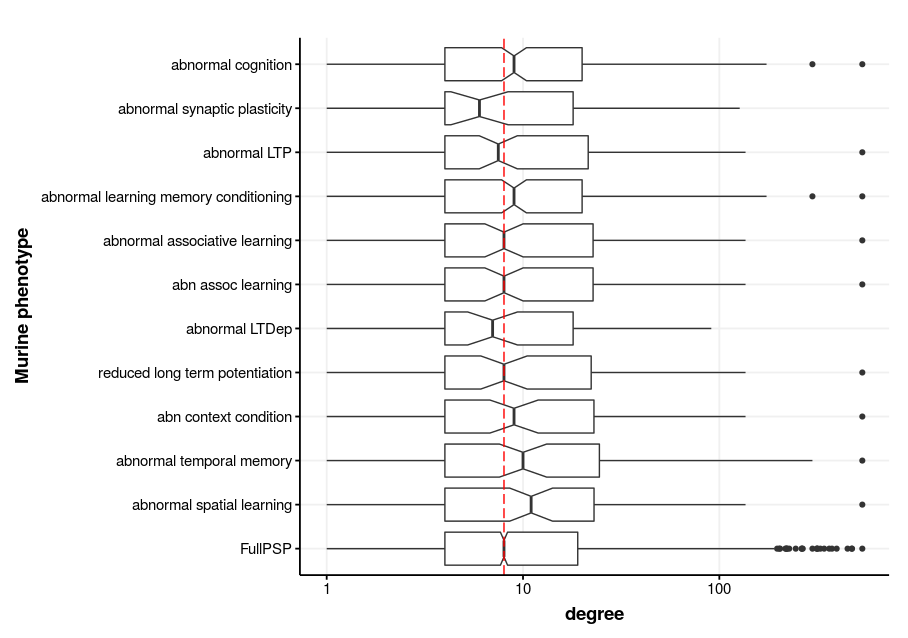
\includegraphics[width=\textwidth]{images/chapter3/ggplot2/murine_centrality_boxplot/add_theme/addLTP/Rplot_murine_degree_ltp.png}
    \caption{Box plot of Degree centrality distribution for differenet gene sets affecting Murine LTP or learning. Log 10 scale for degree. No statistically significant difference other than minor change in long term depression.} 
    \tiny\url{source('~/RProjects/chapter3/R/murine_centrality/general_murine_boxplot/by_measure/degree_centrality_boxplot_murine_ltp_general_degree_add_table.R')}
    \label{fig:murine_ltp_centrality_boxplot_degree1}
\end{figure}


% latex table generated in R 3.6.3 by xtable 1.8-4 package
% Sat Mar 27 14:26:36 2021
% \begin{table}[ht]
% \centering
% \begin{tabular}{rrrrrrrrrr}
%   \toprule
%  & t & df & low & high & mean\_x & mean\_y & stderr & p & p\_BH \\ 
%   \midrule
% abnormal spatial learning & 1.059 & 123.494 & $-4.435 \times 10^{0}$ & $1.463 \times 10^{1}$ & $2.274 \times 10^{1}$ & $1.764 \times 10^{1}$ & $4.817 \times 10^{0}$ & 0.292 & 0.495 \\ 
%   abnormal temporal memory & 1.216 & 108.050 & $-4.514 \times 10^{0}$ & $1.883 \times 10^{1}$ & $2.480 \times 10^{1}$ & $1.764 \times 10^{1}$ & $5.889 \times 10^{0}$ & 0.227 & 0.495 \\ 
%   abn context condition & 0.849 & 95.791 & $-6.739 \times 10^{0}$ & $1.682 \times 10^{1}$ & $2.268 \times 10^{1}$ & $1.764 \times 10^{1}$ & $5.934 \times 10^{0}$ & 0.398 & 0.495 \\ 
%   reduced long term potentiation & 0.758 & 101.013 & $-7.044 \times 10^{0}$ & $1.576 \times 10^{1}$ & $2.200 \times 10^{1}$ & $1.764 \times 10^{1}$ & $5.747 \times 10^{0}$ & 0.450 & 0.495 \\ 
%   abnormal LTDep & -3.232 & 82.756 & $-8.897 \times 10^{0}$ & $-2.119 \times 10^{0}$ & $1.214 \times 10^{1}$ & $1.764 \times 10^{1}$ & $1.704 \times 10^{0}$ & 0.002 & 0.019 \\ 
%   abn assoc learning & 0.864 & 155.249 & $-4.482 \times 10^{0}$ & $1.145 \times 10^{1}$ & $2.113 \times 10^{1}$ & $1.764 \times 10^{1}$ & $4.032 \times 10^{0}$ & 0.389 & 0.495 \\ 
%   abnormal associative learning & 0.864 & 155.249 & $-4.482 \times 10^{0}$ & $1.145 \times 10^{1}$ & $2.113 \times 10^{1}$ & $1.764 \times 10^{1}$ & $4.032 \times 10^{0}$ & 0.389 & 0.495 \\ 
%   abnormal learning memory conditioning & 1.074 & 338.581 & $-2.206 \times 10^{0}$ & $7.516 \times 10^{0}$ & $2.030 \times 10^{1}$ & $1.764 \times 10^{1}$ & $2.471 \times 10^{0}$ & 0.283 & 0.495 \\ 
%   abnormal LTP & 0.463 & 146.622 & $-6.254 \times 10^{0}$ & $1.008 \times 10^{1}$ & $1.956 \times 10^{1}$ & $1.764 \times 10^{1}$ & $4.132 \times 10^{0}$ & 0.644 & 0.644 \\ 
%   abnormal synaptic plasticity & -0.766 & 52.028 & $-9.278 \times 10^{0}$ & $4.149 \times 10^{0}$ & $1.508 \times 10^{1}$ & $1.764 \times 10^{1}$ & $3.346 \times 10^{0}$ & 0.447 & 0.495 \\ 
%   abnormal cognition & 1.074 & 338.581 & $-2.206 \times 10^{0}$ & $7.516 \times 10^{0}$ & $2.030 \times 10^{1}$ & $1.764 \times 10^{1}$ & $2.471 \times 10^{0}$ & 0.283 & 0.495 \\ 
%   \bottomrule
% \end{tabular}
% \caption{Degree murine LTP t test}
% \label{tab:Degre murine LTP. t test}
% \end{table}

None significant see table



\paragraph{betweennness}

High in figure~\ref{fig:murine_ltp_centrality_boxplot_betweenness} abnormal spatial learning (p adj=0.020)m  abnormal cognition 0.026 table~\ref{tab:betweenness murine phenotypes. Wilcoxon test compared with full PSP. P adjusted using B.H}. This may be one of the areas where we see high betweenness areas affected and the general trend is to high betweenness.
\begin{figure}
    \centering
    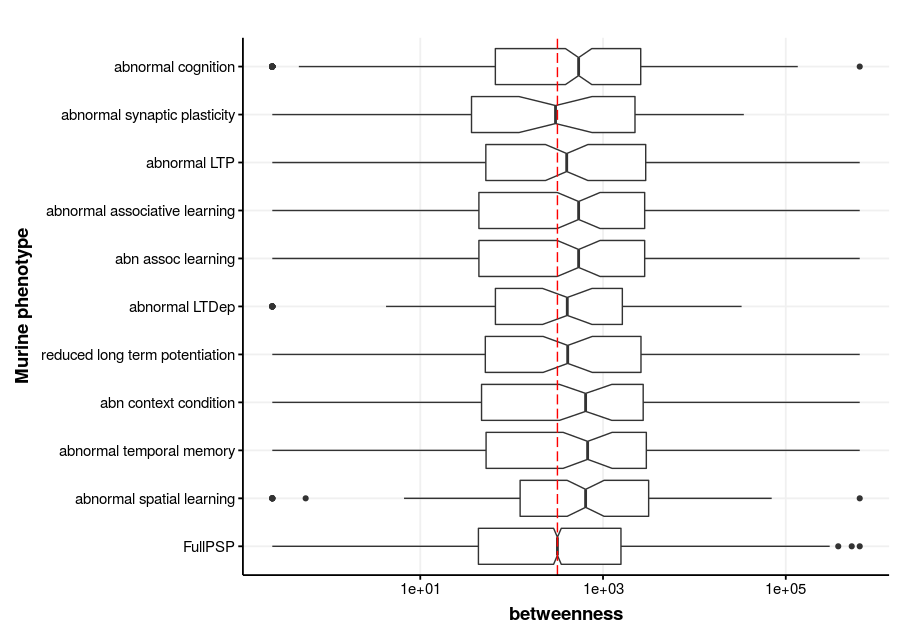
\includegraphics[width=\textwidth]{images/chapter3/ggplot2/murine_centrality_boxplot/add_theme/addLTP/Rplot_betweenness_edit.png}
    \caption{Box plot of betweenness centrality distribution for differenet gene sets affecting Murine LTP or learning. Log 10 scale for betweenness} 
    \tiny\url{source('~/RProjects/chapter3/R/murine_centrality/general_murine_boxplot/rough_centrality_boxplot_murine_ltp_general_closeness.R'}
    \label{fig:murine_ltp_centrality_boxplot_betweenness}
\end{figure}

% latex table generated in R 3.6.3 by xtable 1.8-4 package
% Sat Mar 27 14:40:21 2021
% latex table generated in R 3.6.3 by xtable 1.8-4 package
% Sat Mar 27 14:45:29 2021
% latex table generated in R 3.6.3 by xtable 1.8-4 package
% Sat Mar 27 15:47:08 2021
\begin{table}[ht]
\centering
\begin{tabular}{rlrrll}
  \toprule
 & group2 & p & p.adj & p.signif & method \\ 
  \midrule
1 & abnormal spatial learning & 0.002 & 0.020 & ** & Wilcoxon \\ 
  2 & abnormal temporal memory & 0.042 & 0.340 & * & Wilcoxon \\ 
  3 & abn context condition & 0.114 & 0.570 & ns & Wilcoxon \\ 
  4 & reduced long term potentiation & 0.363 & 1.000 & ns & Wilcoxon \\ 
  5 & abnormal LTDep & 0.750 & 1.000 & ns & Wilcoxon \\ 
  6 & abn assoc learning & 0.058 & 0.410 & ns & Wilcoxon \\ 
  7 & abnormal associative learning & 0.058 & 0.410 & ns & Wilcoxon \\ 
  8 & abnormal LTP & 0.271 & 1.000 & ns & Wilcoxon \\ 
  9 & abnormal synaptic plasticity & 0.946 & 1.000 & ns & Wilcoxon \\ 
  10 & abnormal cognition & 0.003 & 0.026 & ** & Wilcoxon \\ 
   \bottomrule
\end{tabular}
\caption{betweenness murine phenotypes. Wilcoxon test compared with full PSP. P adjusted using B.H} 
\label{tab:betweenness murine phenotypes. Wilcoxon test compared with full PSP. P adjusted using B.H}
\end{table}

\paragraph{Closeness}

Closeness reduced figure~\ref{fig:murine_ltp_centrality_boxplot_closeness}, table~\ref{tab:closeness murine phenotypes. Wilcoxon test compared with full PSP.}, Abnormal LTDepression only significant term after correction for multiple comparisons ($p_{BH}$=0.018).

\begin{figure}
    \centering
    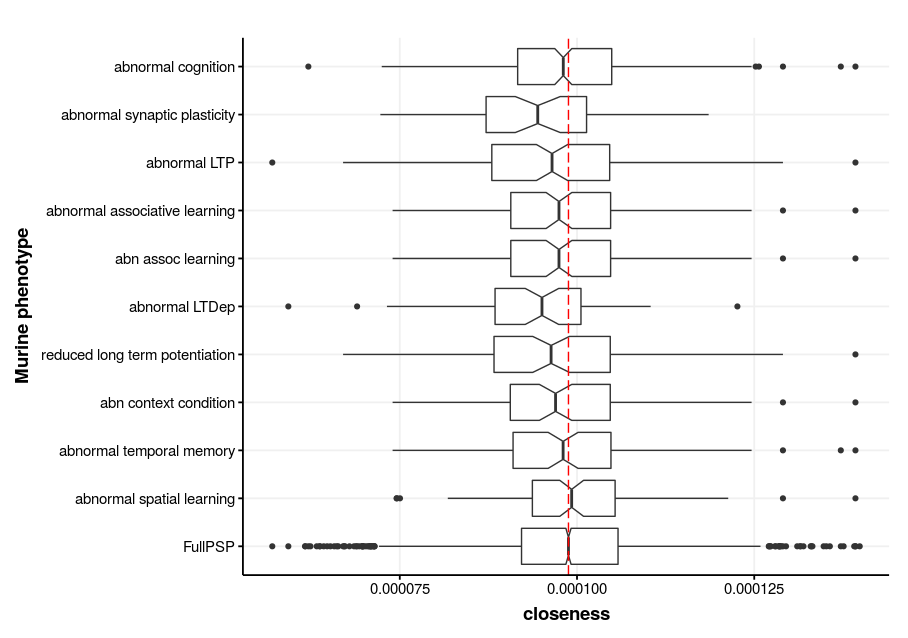
\includegraphics[width=\textwidth]{images/chapter3/ggplot2/murine_centrality_boxplot/add_theme/addLTP/Rplot_closeness_editnolog10.png}
    \caption{Box plot of Closeness centrality distribution for differenet gene sets affecting Murine LTP or learning. Closeness not logarithimic} 
   \tiny\url{source('~/RProjects/chapter3/R/murine_centrality/general_murine_boxplot/by_measure/degree_centrality_boxplot_murine_ltp_general_closeness_add_table.R')}
    \label{fig:murine_ltp_centrality_boxplot_closeness}
\end{figure}

% latex table generated in R 3.6.3 by xtable 1.8-4 package
% Sat Mar 27 15:39:06 2021
\begin{table}[ht]
\centering
\begin{tabular}{rlrrll}
  \toprule
 & group2 & p & p.adj & p.signif & method \\ 
  \midrule
1 & abnormal spatial learning & 0.608 & 1.000 & ns & Wilcoxon \\ 
  2 & abnormal temporal memory & 0.539 & 1.000 & ns & Wilcoxon \\ 
  3 & abn context condition & 0.273 & 1.000 & ns & Wilcoxon \\ 
  4 & reduced long term potentiation & 0.088 & 0.610 & ns & Wilcoxon \\ 
  5 & abnormal LTDep & 0.002 & 0.018 & ** & Wilcoxon \\ 
  6 & abn assoc learning & 0.233 & 1.000 & ns & Wilcoxon \\ 
  7 & abnormal associative learning & 0.233 & 1.000 & ns & Wilcoxon \\ 
  8 & abnormal LTP & 0.047 & 0.370 & * & Wilcoxon \\ 
  9 & abnormal synaptic plasticity & 0.008 & 0.070 & ** & Wilcoxon \\ 
  10 & abnormal cognition & 0.565 & 1.000 & ns & Wilcoxon \\ 
   \bottomrule
\end{tabular}
\caption{closeness murine phenotypes. Wilcoxon test compared with full PSP. P adjusted using B.H} 
\label{tab:closeness murine phenotypes. Wilcoxon test compared with full PSP.}
\end{table}

% \begin{figure}
%     \centering
%     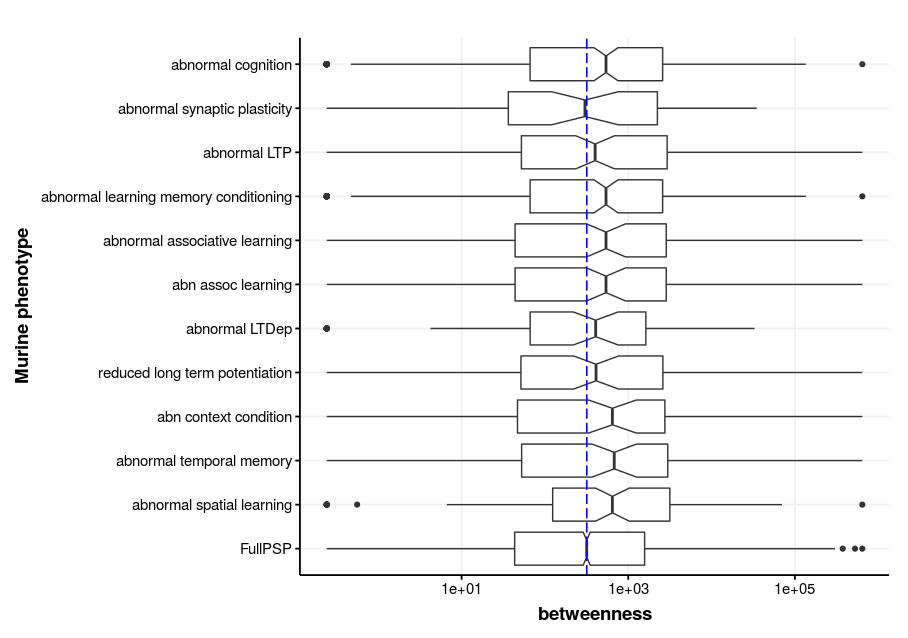
\includegraphics[width=\textwidth]{images/chapter3/ggplot2/murine_centrality_boxplot/add_theme/addLTP/Rplot_theme_add_ltp_corrected_spelling_betweenness.png}
%     \caption{Box plot of Betweenness distribution for differenet gene sets affecting Murine LTP or learning. Log 10 scale for degree.} 
%     \tiny\url{source('~/RProjects/chapter3/R/murine_centrality/general_murine_boxplot/rough_centrality_boxplot_murine_ltp_general_betweenness_add_table.R')}
%     \label{fig:murine_ltp_centrality_boxplot_centrality}
% \end{figure}

% latex table generated in R 3.6.3 by xtable 1.8-4 package
% Fri Mar 26 19:13:36 2021



% latex table generated in R 3.6.3 by xtable 1.8-4 package
% Sat Mar 27 13:07:35 2021
\paragraph{Eigenvector}


Figure~\ref{fig:murine_ltp_centrality_boxplot_eigenvector} and table~\ref{tab:eigencentrality murine phenotypes. Wilcoxon test compared with full PSP}. Abnormal synaptic plasticity and abnormal long term depression have reduced eigenvector centrality. 

This pattern may reflect that animal phenotypes have affected receptors on the periphery of the network
\begin{figure}
    \centering
    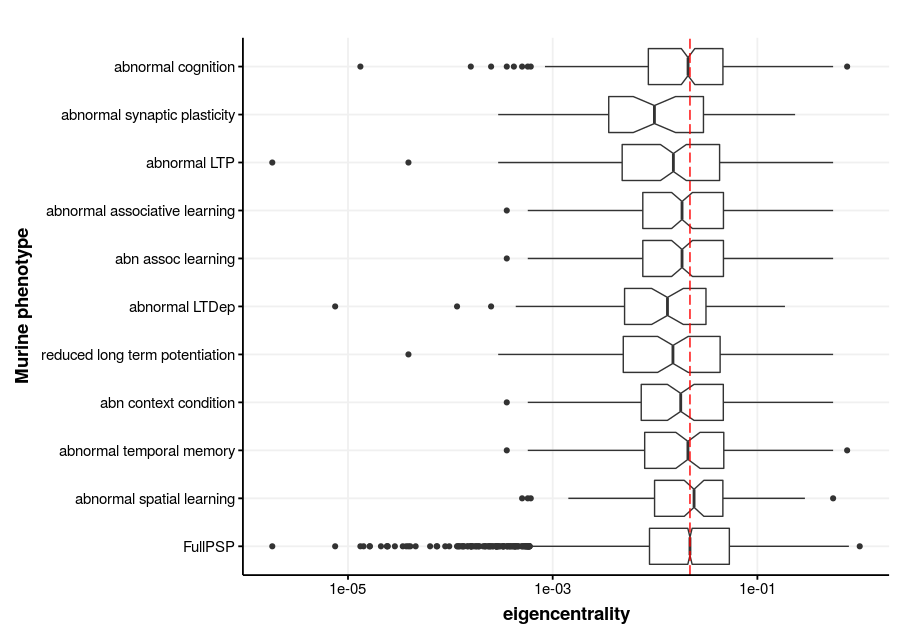
\includegraphics[width=\textwidth]{images/chapter3/ggplot2/murine_centrality_boxplot/add_theme/addLTP/Rplot_eigen_edit.png}
    \caption{Box plot of Eigenvector centrality distribution for differenet gene sets affecting Murine LTP or learning. Log10} 
   \tiny\url{source('~/RProjects/chapter3/R/murine_centrality/general_murine_boxplot/by_measure/degree_centrality_boxplot_murine_ltp_general_eigenvector_add_table.R')}
    \label{fig:murine_ltp_centrality_boxplot_eigenvector}
\end{figure}


% latex table generated in R 3.6.3 by xtable 1.8-4 package
% Sat Mar 27 15:56:24 2021
\begin{table}[ht]
\centering
\begin{tabular}{rlrrll}
  \toprule
 & group2 & p & p.adj & p.signif & method \\ 
  \midrule
1 & abnormal spatial learning & 0.926 & 1.000 & ns & Wilcoxon \\ 
  2 & abnormal temporal memory & 0.592 & 1.000 & ns & Wilcoxon \\ 
  3 & abn context condition & 0.321 & 1.000 & ns & Wilcoxon \\ 
  4 & reduced long term potentiation & 0.053 & 0.370 & ns & Wilcoxon \\ 
  5 & abnormal LTDep & 0.002 & 0.021 & ** & Wilcoxon \\ 
  6 & abn assoc learning & 0.229 & 1.000 & ns & Wilcoxon \\ 
  7 & abnormal associative learning & 0.229 & 1.000 & ns & Wilcoxon \\ 
  8 & abnormal LTP & 0.012 & 0.097 & * & Wilcoxon \\ 
  9 & abnormal synaptic plasticity & 0.002 & 0.021 & ** & Wilcoxon \\ 
  10 & abnormal cognition & 0.338 & 1.000 & ns & Wilcoxon \\ 
   \bottomrule
\end{tabular}
\caption{eigencentrality murine phenotypes. Wilcoxon test compared with full PSP. P adjusted using B.H} 
\label{tab:eigencentrality murine phenotypes. Wilcoxon test compared with full PSP}
\end{table}
\paragraph{transitivity}

transitivity not significant


\paragraph{kcoreness and mouse ltp}
kcoreness not significant\footnote{\url{source('~/RProjects/chapter3/R/murine_centrality/general_murine_boxplot/rough_centrality_boxplot_murine_ltp_general_kcoreness_add_table.R')}}


\paragraph{Betweenness centrality}
% latex table generated in R 3.6.3 by xtable 1.8-4 package
% Sat Mar 27 13:33:11 2021
% latex table generated in R 3.6.3 by xtable 1.8-4 package
% Sat Mar 27 13:35:54 2021







\clearpage



\section{Disease enrichment for centrality measures}

Disgennet2r tables moved to section~\ref{sec:disgennet2r tables}



\subsection{Results Feb DisGen ToppGENE}
\subsubsection{Degree}
\paragraph{High}
% latex table generated in R 3.6.3 by xtable 1.8-4 package
% Tue Mar 16 12:09:01 2021
\begin{table}[ht]
\centering

\setlength{\extrarowheight}{2pt}
\begin{adjustbox}{width=\textwidth}

\begin{tabular}{lllllll}
  \toprule
 & ID & Name & $n$ PSP & $n$ set & $p$ & q FDR B.H \\ 
  \midrule
1 & C0002736 & Amyotrophic Lateral Sclerosis & 354 & 85 & $8.152 \times 10^{-15}$ & $5.720 \times 10^{-12}$ \\ 
  2 & C0338451 & Frontotemporal dementia & 119 & 40 & $4.413 \times 10^{-12}$ & $1.081 \times 10^{-9}$ \\ 
  3 & C0236642 & Pick Disease of the Brain & 89 & 32 & $9.642 \times 10^{-11}$ & $1.429 \times 10^{-8}$ \\ 
  4 & C0949664 & Tauopathies & 91 & 31 & $9.233 \times 10^{-10}$ & $1.114 \times 10^{-7}$ \\ 
  5 & C1843013 & Alzheimer disease, familial, type 3 & 57 & 22 & $2.097 \times 10^{-8}$ & $1.536 \times 10^{-6}$ \\ 
  6 & C0524851 & Neurodegenerative Disorders & 484 & 88 & $3.194 \times 10^{-8}$ & $2.276 \times 10^{-6}$ \\ 
  7 & C0014057 & Japanese Encephalitis & 30 & 15 & $6.448 \times 10^{-8}$ & $4.284 \times 10^{-6}$ \\ 
  8 & C0751072 & Frontotemporal Lobar Degeneration & 81 & 26 & $9.075 \times 10^{-8}$ & $5.692 \times 10^{-6}$ \\ 
  9 & C0040997 & Trigeminal Neuralgia & 17 & 11 & $1.147 \times 10^{-7}$ & $7.139 \times 10^{-6}$ \\ 
  10 & C0004114 & Astrocytoma & 255 & 54 & $1.805 \times 10^{-7}$ & $1.040 \times 10^{-5}$ \\ 
  11 & C0220756 & Niemann-Pick Disease, Type C & 45 & 18 & $2.235 \times 10^{-7}$ & $1.231 \times 10^{-5}$ \\ 
  12 & C0020179 & Huntington Disease & 271 & 56 & $2.491 \times 10^{-7}$ & $1.347 \times 10^{-5}$ \\ 
  13 & C0006118 & Brain Neoplasms & 245 & 52 & $2.930 \times 10^{-7}$ & $1.552 \times 10^{-5}$ \\ 
  14 & C4551993 & Amyotrophic Lateral Sclerosis, Familial & 37 & 16 & $2.982 \times 10^{-7}$ & $1.566 \times 10^{-5}$ \\ 
  15 & C4024896 & Motor neuron atrophy & 55 & 20 & $2.996 \times 10^{-7}$ & $1.566 \times 10^{-5}$ \\ 
  16 & C0027765 & nervous system disorder & 289 & 56 & $2.308 \times 10^{-6}$ & $8.785 \times 10^{-5}$ \\ 
  17 & C0002622 & Amnesia & 49 & 17 & $5.056 \times 10^{-6}$ & $1.680 \times 10^{-4}$ \\ 
  18 & C0009241 & Cognition Disorders & 173 & 38 & $5.876 \times 10^{-6}$ & $1.927 \times 10^{-4}$ \\ 
  19 & C0026837 & Muscle Rigidity & 65 & 20 & $6.135 \times 10^{-6}$ & $2.004 \times 10^{-4}$ \\ 
  20 & C4552000 & Episodic Kinesigenic Dyskinesia 1 & 53 & 17 & $1.682 \times 10^{-5}$ & $4.866 \times 10^{-4}$ \\ 
   \bottomrule
\end{tabular}
\end{adjustbox}
\caption{Disease enrichment for neurological disorders using the 90th centile of degree distribution compared with a background set of all PSP genes. Correction for multiple comparisons by Benjamini and Hochberg method (q FDR BH). Twenty most enriched gene sets shown ordered by $q$ FDR. The number of genes annotated to the disease term in the PSP is $n$ PSP and the number in the top 90th centile of genes by degree in PSP is $n$ set } 
\tiny\url{source('~/RProjects/chapter3/R/toppgene_disgen/xtable/output_high_degree.R')}

\end{table}
% latex table generated in R 3.6.3 by xtable 1.8-4 package
% Tue Mar 16 12:09:01 2021
\begin{table}[ht]
\centering

\setlength{\extrarowheight}{2pt}
\begin{adjustbox}{width=\textwidth}

\begin{tabular}{lllllll}
  \toprule
 & ID & Name & n PSP & n set & $p$ & q FDR B.H \\ 
  \midrule
1 & C0042769 & Virus Diseases & 332 & 95 & $1.434 \times 10^{-22}$ & $1.124 \times 10^{-18}$ \\ 
  2 & C0019163 & Hepatitis B & 290 & 82 & $6.045 \times 10^{-19}$ & $2.370 \times 10^{-15}$ \\ 
  3 & C2931822 & Nasopharyngeal carcinoma & 294 & 80 & $2.383 \times 10^{-17}$ & $6.228 \times 10^{-14}$ \\ 
  4 & C0026764 & Multiple Myeloma & 341 & 85 & $7.091 \times 10^{-16}$ & $1.390 \times 10^{-12}$ \\ 
  5 & C0024299 & Lymphoma & 300 & 77 & $4.178 \times 10^{-15}$ & $5.720 \times 10^{-12}$ \\ 
  6 & C0302592 & Cervix carcinoma & 352 & 85 & $5.658 \times 10^{-15}$ & $5.720 \times 10^{-12}$ \\ 
  7 & C0033578 & Prostatic Neoplasms & 175 & 55 & $6.894 \times 10^{-15}$ & $5.720 \times 10^{-12}$ \\ 
  8 & C0007847 & Malignant tumor of cervix & 315 & 79 & $6.963 \times 10^{-15}$ & $5.720 \times 10^{-12}$ \\ 
  9 & C0002736 & Amyotrophic Lateral Sclerosis & 354 & 85 & $8.152 \times 10^{-15}$ & $5.720 \times 10^{-12}$ \\ 
  10 & C1332977 & Childhood Leukemia & 367 & 87 & $8.194 \times 10^{-15}$ & $5.720 \times 10^{-12}$ \\ 
  11 & C0079731 & B-Cell Lymphomas & 273 & 72 & $8.656 \times 10^{-15}$ & $5.720 \times 10^{-12}$ \\ 
  12 & C0023418 & leukemia & 407 & 93 & $8.755 \times 10^{-15}$ & $5.720 \times 10^{-12}$ \\ 
  13 & C1832661 & Anopthalmia and pulmonary hyp. & 298 & 76 & $9.684 \times 10^{-15}$ & $5.840 \times 10^{-12}$ \\ 
  14 & C4048328 & cervical cancer & 340 & 82 & $2.147 \times 10^{-14}$ & $1.202 \times 10^{-11}$ \\ 
  15 & C0040136 & Thyroid Neoplasm & 231 & 64 & $2.877 \times 10^{-14}$ & $1.503 \times 10^{-11}$ \\ 
  16 & C3539878 & Triple Negative Breast Neoplasms & 351 & 82 & $1.510 \times 10^{-13}$ & $7.399 \times 10^{-11}$ \\ 
  17 & C0476089 & Endometrial Carcinoma & 283 & 71 & $2.256 \times 10^{-13}$ & $1.040 \times 10^{-10}$ \\ 
  18 & C0007103 & Malignant neoplasm of endometrium & 229 & 62 & $2.523 \times 10^{-13}$ & $1.099 \times 10^{-10}$ \\ 
  19 & C0007115 & Malignant neoplasm of thyroid & 195 & 56 & $2.950 \times 10^{-13}$ & $1.141 \times 10^{-10}$ \\ 
  20 & C0019196 & Hepatitis C & 362 & 83 & $3.195 \times 10^{-13}$ & $1.141 \times 10^{-10}$ \\ 
   \hline
\end{tabular}
\end{adjustbox}
\caption{Top 20 all disorders 90th centile degree} 
\tiny\url{source('~/RProjects/chapter3/R/toppgene_disgen/xtable/output_high_degree.R')}
\end{table}

\subsection{Moved from toppgene section}
\subsection{Degree Others}
Human phenotype number two is fronto temporal dementia, also includes abormal emotion in table~\ref{tab:ToppGENE Human Phenotype. 90 centile cwpsp.txtp = p value; q FDR B H = q adjusted significance level False Discovery Rate using Benjamini and Hochberg adjustment; n= n genes annotated in test group; n PSP= n genes annotated in PSP. n significant in category 131}.

Mouse phenotype abnormal cell proliferation.

Significant diseases numerous include neoplasms and viral processes. The most significant neuropsychiatric disorder is the 9th term C0002736;  Amyotrophic Lateral Sclerosis; n in high degree 85 and n in PSP 354 p $8.15 \times 10^{-15}$ FDR q $5.72 \times 10^{-12}$. Amyotrophic lateral sclerosis is a neurodegenerative disorder characterised by muscular weakness. It is part of a common disease spectrum with fronto-temporal dementia (see Wikipedia and do cross ref) 





\clearpage

\subsection{Centrality measures and pLI}

The higher centrality measures are the higher is the probability of loss of function intolerance. The relationship is  moderately strong for all centrality measures other than transitivity see table~\ref{tab:Correlation of Centrality measures with probability of loss of function intolerance (pLI) gnomad.}
% latex table generated in R 3.6.3 by xtable 1.8-4 package
% Sun Oct 18 17:25:49 2020
\begin{table}[ht]
\centering
\begin{tabular}{rrrr}
  \hline
 & S & rho & p \\ 
  \hline
degree & $5.14 \times 10^{9}$ & 0.225 & $2.37 \times 10^{-40}$ \\ 
  betweenness\_centrality & $5.29 \times 10^{9}$ & 0.202 & $1.29 \times 10^{-32}$ \\ 
  eigenvector & $5.21 \times 10^{9}$ & 0.213 & $2.59 \times 10^{-36}$ \\ 
  closeness & $5.14 \times 10^{9}$ & 0.225 & $2.20 \times 10^{-40}$ \\ 
  transitivityNA & $4.54 \times 10^{9}$ & 0.097 & $5.66 \times 10^{-8}$ \\ 
  kcoreness & $5.10 \times 10^{9}$ & 0.231 & $1.95 \times 10^{-42}$ \\ 
   \hline
\end{tabular}
\caption{Correlation of Centrality measures with probability of loss of function intolerance (pLI) gnomad.\url{source('~/RProjects/db_essential_genes/R/gnomad/correlation/correlation_gnomad/pLI_graph/cor_pLI_and_graph.R')}} 
\label{tab:Correlation of Centrality measures with probability of loss of function intolerance (pLI) gnomad.}
\end{table}


\section{Summary of chapter}

We show that in the PSP nodes of very high centrality are associated with essentialness. The PSP has a high degree of essentialness compared to the rest of the genome. 

High degree nodes are associated with specific phenotypes and specific gene ontology terms however the are not correlated with genetic differences that are enriched for differences in intelligence. This is not obvious before the fact and is different from other traits eg essentialness. One might hypothesis that the reason is that there is either no effect (ie it is irrelevant) or that in population studies genes with high centrality are more likely to be essential and hence have less genetic variation. We find also in one of the principle animal models of learning murine long term potentiation that genes of high importance were no more likely or less likely to be involved in long term potentiation.

We used data from the Exac project to further investigate whether high importance nodes were subject to selection pressure such that they proved more intolerant of non synonymous genetic changes. Nodes with high degree are associated with an increased probability of being intolerant to changes. 

Nodes with high betweenness centrality were involved in neuro-degenerative disorders including Parkinson's disease see section~\ref{sec:Betweeness centrality}. They were also associated with severe phenotypes in murine models including phenotypes incompatibly with viability. Low betweenness centrality was associated with abnormalities in synaptic transmission in murine models. 

High eigenvector centrality is again associated with severe murine phenotypes and enrichment for RNA and cadherin binding. Disease enrichment is of neoplasms and neurodegenerative disorders. 

Low eigenvector centrality (10\%) were enriched for human phenotypes of seizures and ontology terms of transmitter, mouse phenotype was of abnormal synaptic transmission. The top five enriched disorders in disGeNET were seizure related. 

Despite this there was no association between node centrality measures and the significance of genetic variants for differences in intelligence and educational attainment.

There is a complex relationship between transitivity and degree for nodes with degree 3 or less the correlation is positive and results in a positive overall correlation despite a plot of the relationship appearing clearly negative. This is due to the large number of low degree nodes. When the correlation is calculated for higher degree the relationship previously commented upon in the literature \cite{newman} p 335 is seen. Caution should therefore be used in determining linear correlations involving transitivity especially in smaller networks and it may be prudent to plot the correlation against minimum degree.


\subsubsection{Extra discussion}

I have not included the Weibull as it seems implausible

The number of different factors that affect assortativity are going to play a role in any probabilistic model of a graph and in community formation

Note all report assortativity for example with random estimate

Generating mechanism of the lognormal is multiplication of random vvariables and is more common as dimensions increase above one dimension \cite{} ?discussion \cite{koch1966logarithm}
\cite{limpert2001log}

$C_k$ correlation misleading if not taken with $x_{min}$ like method

\textcolor{red}{The literature MOVE TO DISCUSSION} records a decrease in the average value of the clustering coefficient with increasing $k$. This has been done mostly for large networks such as the internet \cite{newman2018networks} p 335.
This relationship between $k$ and the transitivity $C$ therefore probably holds true in large networks (such as the internet where the studies were performed) where the number of nodes of low degree is dominated by the number of high degree (in this case $>=5$ nodes). 

\paragraph{Degree and local transitivity}
\label{sec:discuss degree and local transitivity - summary just now}
Reviewing the previous literature on the correlation between degree and local clustering Ravasz and Barabasi in a highly cited work \cite{ravasz2002hierarchical} review a generative model of high clustering coefficient and scale free degree distribution and real world networks. The real world networks include the actor network (392,340 nodes), the language network based on synonyms in Merriams English dictionary (182,853 nodes), the world wide web from mapping out from the \url{www.nd.edu} domain with 325,729 nodes, the internet at the router level (260,657 nodes) and the power grid of the Western United states 4941 nodes 13188 edges. \textcolor{red}{end move to discussion}

These networks are all large and in the logarithmic graphs of clustering coefficient and degree the minumum degree starts around 10. It is interesting to note in figure 4 \textcolor{red}{of what pressumably Ravasz and Barabasi?} showing the internet at router level and power network there are lower degree nodes but the slope of the line representing the correlation coefficient is dominated by the effect of high degree nodes and the distribution of clustering coefficient in the lower degree domain is quite different. These matters may seem small as for large degree the overall pattern holds but it is a useful practical fact to be aware of if we are testing the association of clustering coefficient with another variable in smaller networks such as the PSP which is not readily apparent from the literature.

(Although in measuring the correlation of transitivty with another measure you are still measuring its correlation but a high transitivity low degree region may have different behaviour in the network to the majority degree greater than 10 negative correlation with transitivity)\\todo{correlation both domains}

\section{???tmp???}
 \subsection{***Results from database of essential genes}
 \todo{difference plI and DEG}
 Most up to date data:
43294 entries in all

32578 human 

8973 genes

number of genes in NCBI37.3 8973
8973/19427 = 46.1\%

15987 genes NCBI non synaptic
6616

2328 genes in PSP 67.3\%

6616/15987 41.4\% of genes not in PSP






%https://tex.stackexchange.com/questions/508546/help-fixing-a-contingency-table?noredirect=1&lq=1

% latex table generated in R 3.6.3 by xtable 1.8-4 package
% Wed Mar 17 18:22:08 2021



   


\paragraph{Previous data}
2238 genes in the PSP are essential (64.7\%)

This compares with 37.\% of the genome as a whole (assuming 20000 genes \todo{get non essential number from database}. 36.5\% (6043/20000) non PSP genes are essential. 

\subsubsection{Degree and essential genes}

The summary statistics for the degree of essential PSP genes and non essential PSP genes are shown in table~\ref{tab:degree distribution essential and non essential genes PSP}. The mean degree is higher in essential (21.29) vs non essential genes (10.94) $p<2.2 \time 10^{-16}   W=1777916$ Wilcoxon rank sum test with continuity correction in R.

The boxplot of log degree for essential and non essential genes in the PSP is shown in figure~\ref{fig:boxplot_log degree essential genes}
\footnote{code \url{source('~/RProjects/paper_xls_latex/R/essentail_genes/lbxplot_and_latex_essential_genes.R')}}.

The assortativity of essential nodes in the PSP is 0.0438 (ie very mild assortative although they tend to have high degree and PSP degree is disassortative).


\begin{table}[ht]
\centering
\begin{tabular}{rlrrrrrrr}
  \hline
 & name & n & Min. & 1st Qu. & Median & Mean & 3rd Qu. & Max. \\ 
  \hline
1 & Essential & 2238 & 1.00 & 5.00 & 11.00 & 21.29 & 23.00 & 474.00 \\ 
  2 & Non essential & 1219 & 1.00 & 2.50 & 5.00 & 10.94 & 12.00 & 535.00 \\ 
  3 & All & 3457 & 1.00 & 4.00 & 8.00 & 17.64 & 19.00 & 535.00 \\ 
   \hline
\end{tabular}
\caption{Degree distribution of essential and non essential genes in PSP}
\label{tab:degree distribution essential and non essential genes PSP}
\end{table}




\begin{figure}
    \centering
    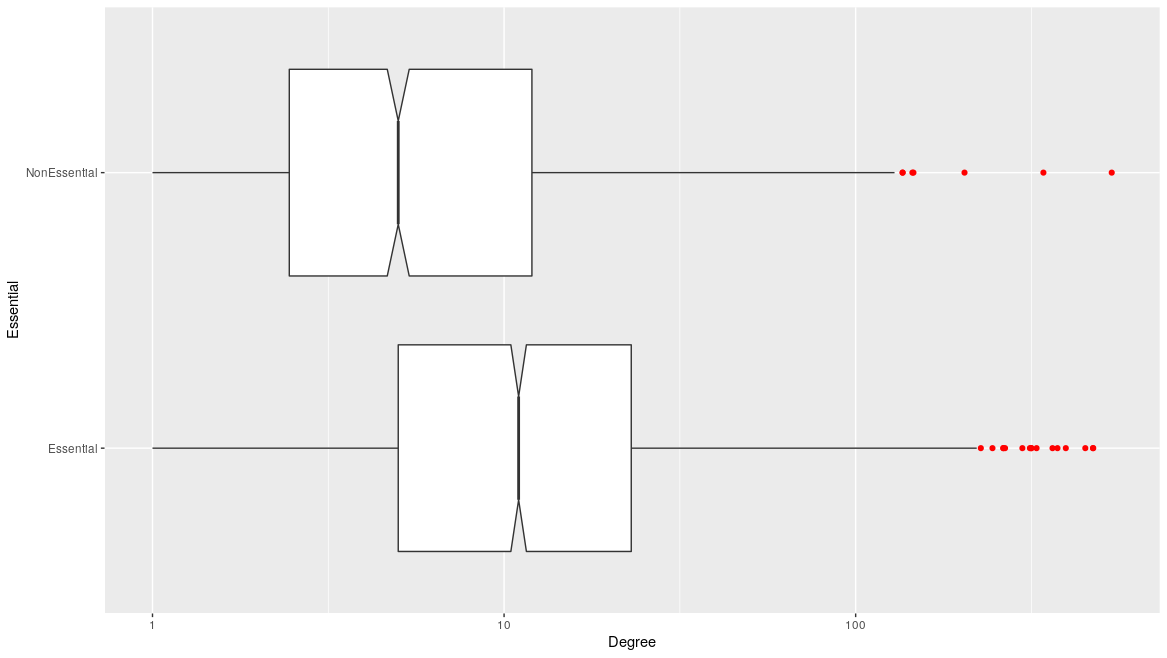
\includegraphics[width=\textwidth]{images/Rplot_essential_non_essential_gene_degree.png}
    \caption{Degree distribution for essential and non essential PSP genes using DEG 15.2. 2238 Essential genes, 1219 Non essential}
    \label{fig:boxplot_log degree essential genes}
\end{figure}



\subsection{Redo}
Have done degree and all centrality measures with essential genes \url{source('~/RProjects/chapter3/R/essential_genes/load_essential_genes.R')}

Closeness and transitivity not log
\subsection{***Feb redo: Synaptic and essential genes}

     Finding genes in five or more studies  
     
     Total genes 8992  
     
     Number of studies: 20.              20 according to website in most recent update  
     
     Number of genes appearing in 5 or more studies 2178  
     
     Number of synaptic genes in DEG 2328  
     
     Number of synaptic genes in 5 or more studies 728  
     
      Number of non synaptic ie NCBI 37 genes 15987
      
     Number of non synaptic ie NCBI 37 genes (so eligible for study)             in DEG 6620  
     
     Number of non synaptic ie NCBI 37 genes (so eligible for study)             in five or more studies 1444  
     
     Synaptic genes in NCBI 37 3440  
     
     Percentage of synaptic genes in DEG in five or more 31.27 \%  
     
     Percentage of non synaptic genes in DEG in five or more 21.81 \% 
     
     Percent of NCBI synaptic 17.71 \%  
     
     Percent of DEG synaptic 25.89 \%  
     
     Percent of greater than 5 synaptic 33.43 \% 
     
     \footnote{source for above \url{source('~/RProjects/db_essential_genes/R/get_essential_genes/db_2020/findforfive/get_db_essential_greater_five_results_xtable.R')}}
  
  
  
 \subsubsection{***Degree distribution of PSP genes - murine model}
 
 We can use the mouse phenotype ontology to identify essential murine genes. 
 We want to know if high degree PSP nodes are more commonly associated with essentiality in murine models. 
 
 The 90\% centile for PSP gene degree is $k=37$. 349 genes in the PSP network model have degree $k>=37$.
 
 Murine phenotype MP:008763 is embryonic lethality. 117 of the genes with degree $k>=37$ are essential (33.5\% of 349 genes). 458 genes are essential in the remaining PSP nodes ($k < 37$, 458 of 3108 14.7\%). p $3.13 \times 10^{-11}$ Fisher's exact test for count data R. Odds ratio 2.27 95\% CI 1.79-2.88. \footnote{code:\url{/home/grant/RProjects/phenome_and_network/R/get_degree_90_quantile_PSP.R}} \todo{Calculate difference in degree for essential versus not essential} Comment \todo{one reason for testing the top 10\% is that the degree distribution is of a few hubs (cite Jeong) with different properties from the rest given the scale free structure of the network}
 
 \begin{table}[h]
     \centering
     \begin{tabular}{llllll}
          Title & $k$& n essential & n & percentage essential & p   \\
          \hline
          Top 10\% & $>=37$ & 117 & 349 & 33.5 & $3.13 \times 10^{-11}$\\
          Rest & $<37$ & 458 & 3108 & 14.7 & \\
     \end{tabular}
     \caption{Association of high degree nodes with being essential in murine models. Genes with degree in top 10\% of PSP compared with the rest. P Fisher's Exact Test for Count data.}
     \label{Table:Degree and murine essentialness PSP}
 \end{table}
 

\todo{GO enrichment with background PSP for high degree are in \url{/home/grant/Dropbox/stront_share/data/GO\_high\_degree_psp_background}}


\subsubsection{Centrality and pLI}
The current results suggest that the relationship between the variables is as shown in the factor graph in figure \ref{Figure:Factor graph for relationship between pLI, vertex statistic and study p values}

\begin{figure}
    \centering
    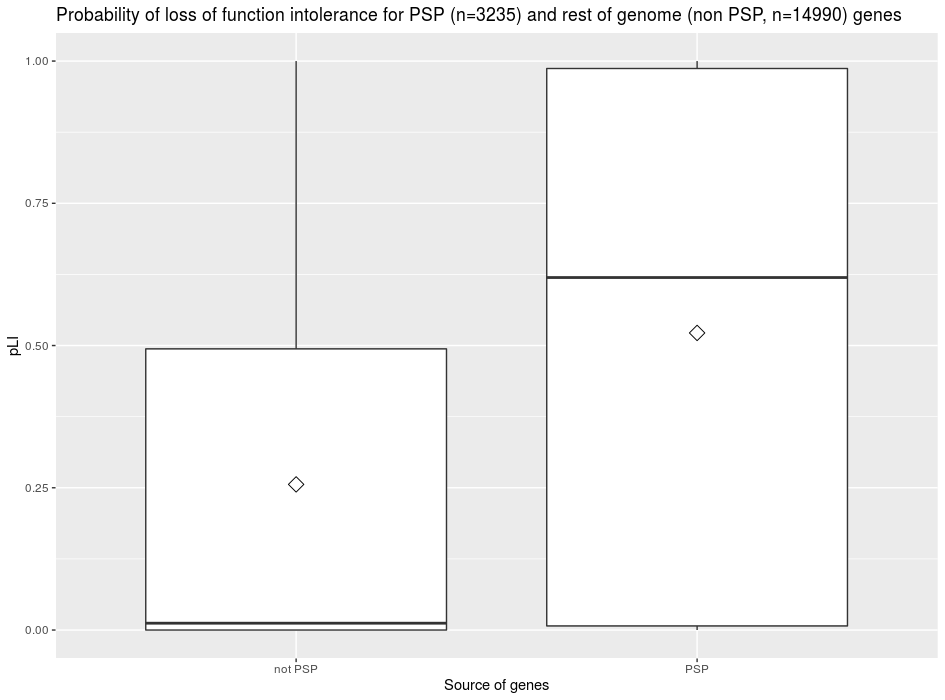
\includegraphics[width=0.9\textwidth]{images/Rplot03_boxplot_pLI_PSP_non_PSP.png}
    \caption{Box plot of probability of loss of function intolerance (pLI) between PSP genes (n=) and non PSP genes (rest of genome n=14990 ). Diamond marker indicates mean PSP value. }
    \label{fig:Boxplot of pli}
\end{figure}

\begin{figure}
    \centering
    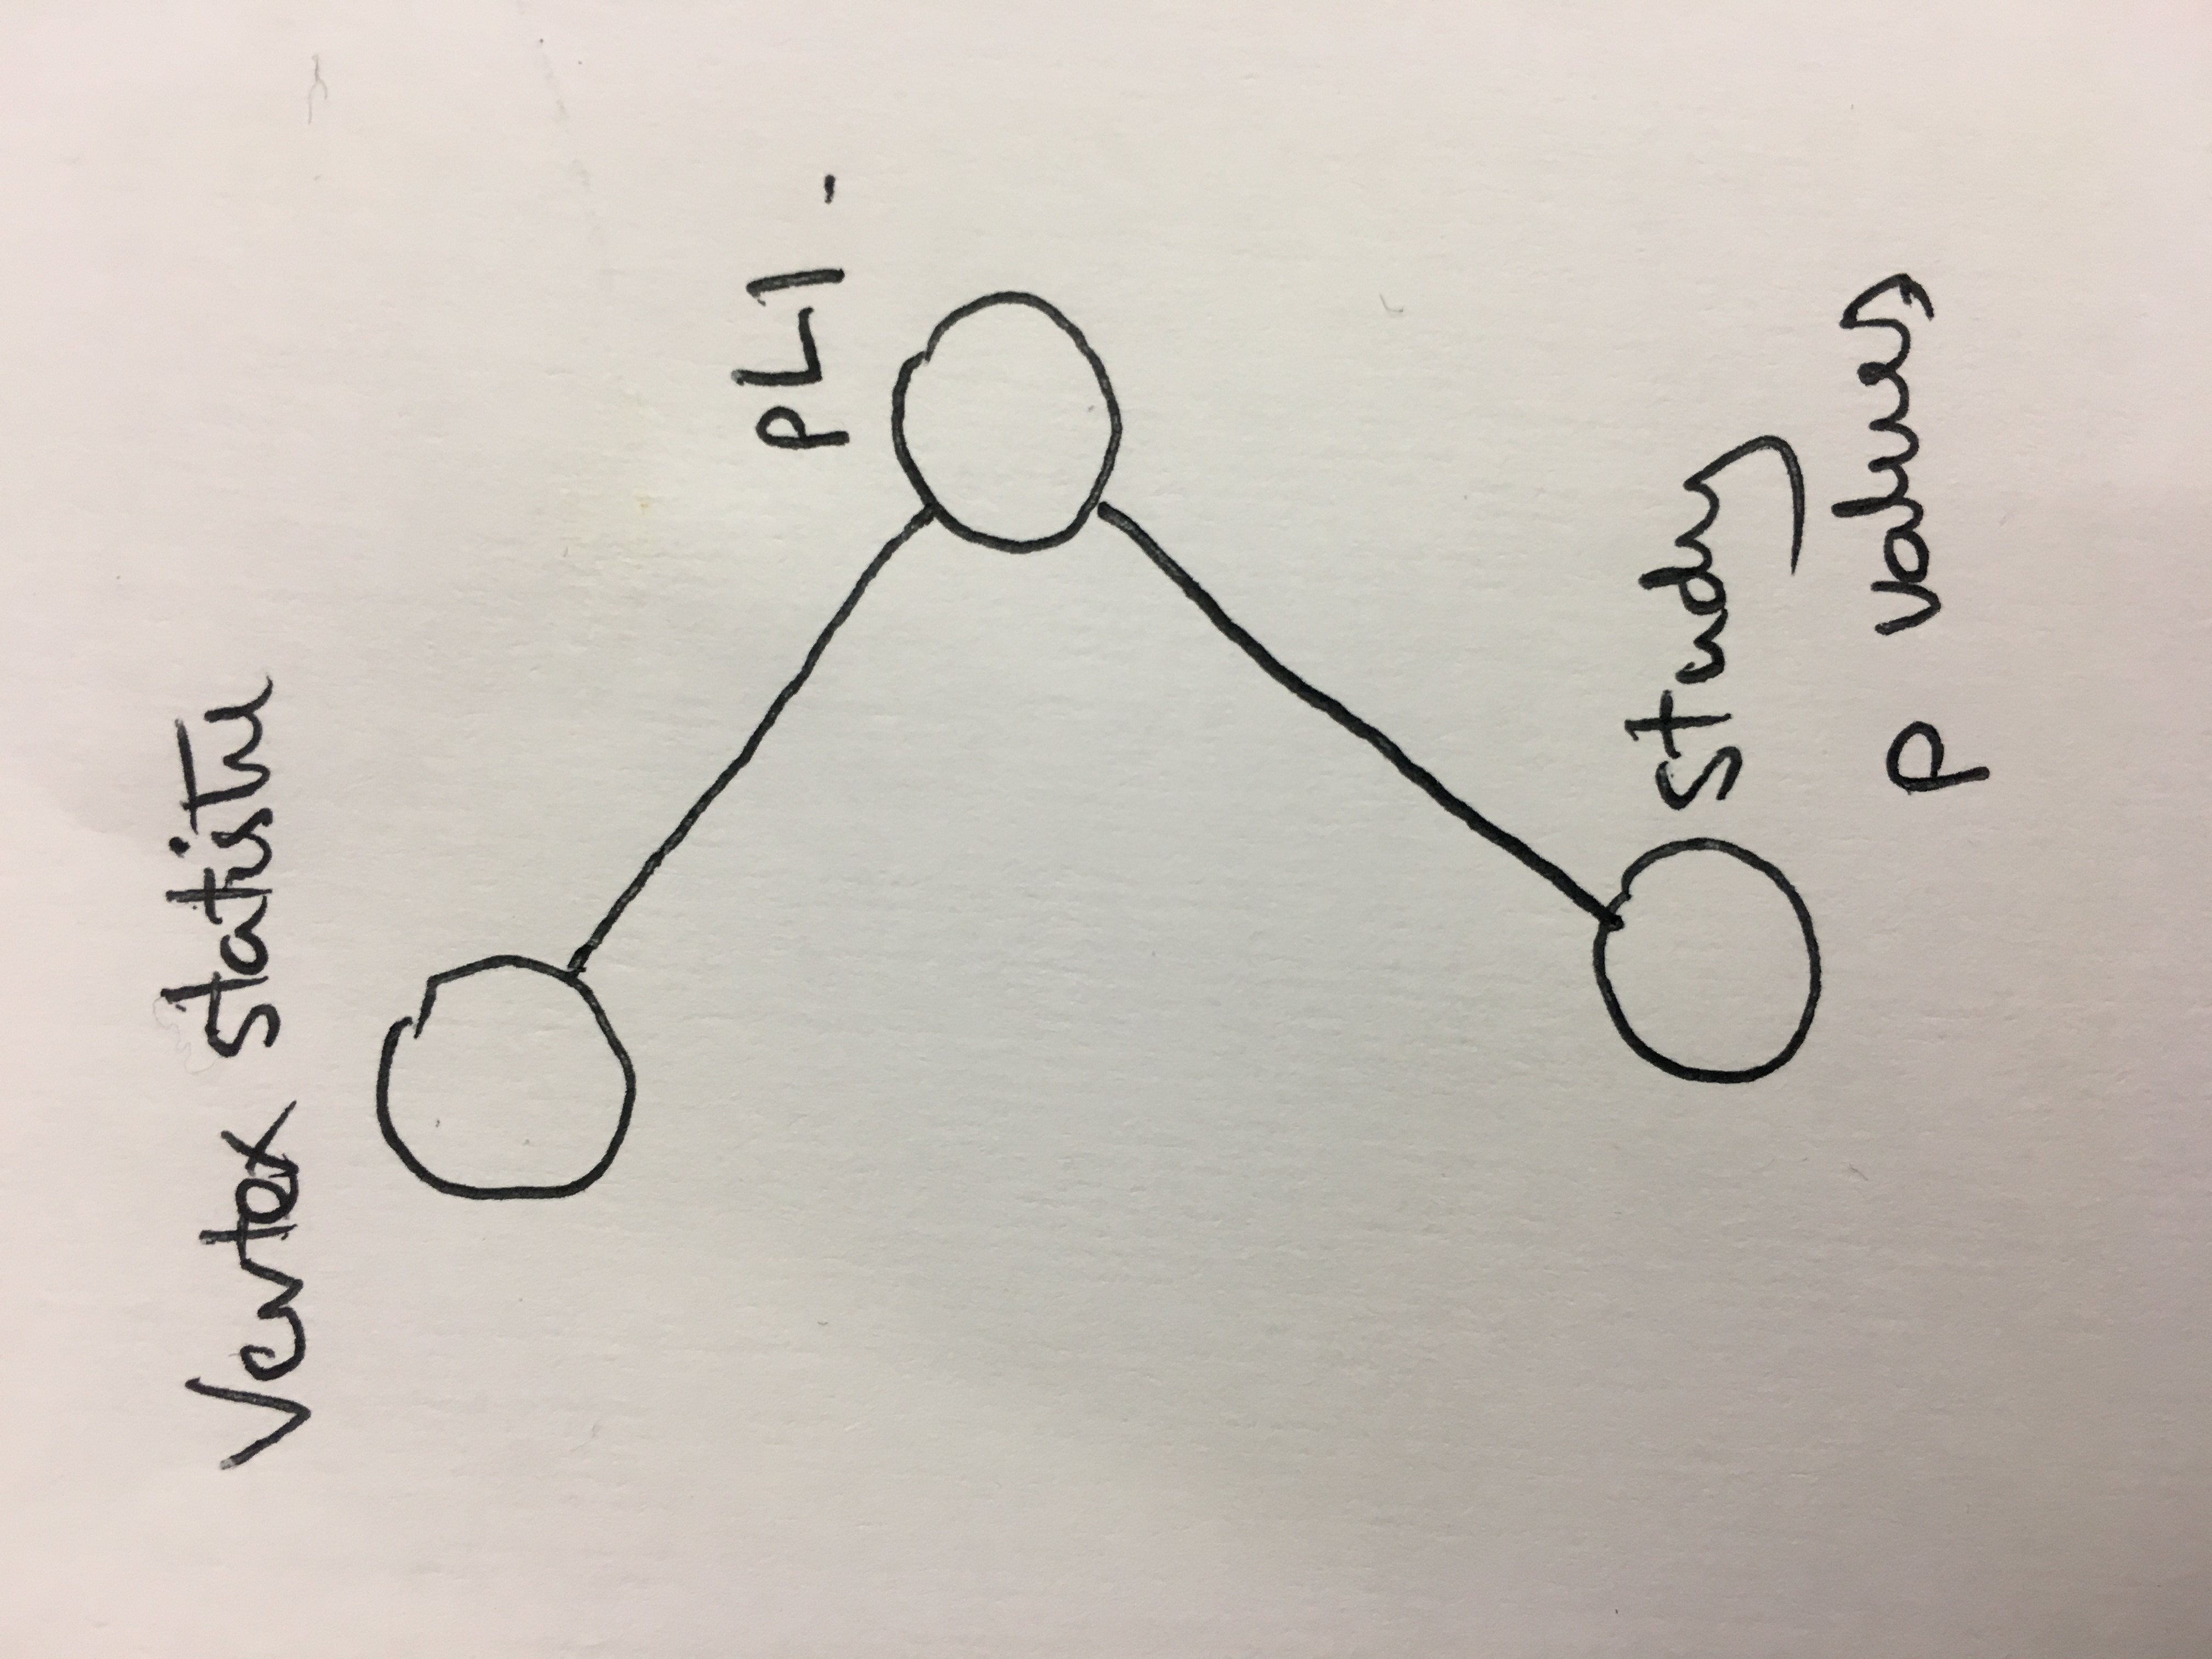
\includegraphics[width=\textwidth]{IMG_6979.JPG}
    \caption{Factor graph for relationship between pLI, vertex statistic and study p values}
    \label{Figure:Factor graph for relationship between pLI, vertex statistic and study p values}
\end{figure}
\todo{Make into table}

 
 The march redo is in table~\ref{tab:correlation pli vertex statistics mar}
 
  

\paragraph{Non march}
There was a positive correlation between loss of function intolerance and the gene Z stat. To be explicit the Z stat is high and positive when the gene has a more significant association with the phenotype and hence a lower p value. There is a weak association between high loss of function intolerance and significant (low p value genes)

\todo{there is something wrong here as Jan we find correlation} 
 In testing correlation spearman’s rank correlation was used as the distribution of the probability of loss of function intolerance statistic is very non linear. It has a bi-modal distribution (see figure~\ref{fig:density estimate pLi}) with a concentration of probability mass around 0 and 1 .


The distribution of probabilitity of loss of function intolerance in non PSP genes is still bimodal but the probability mass around 1 is much less peaked and there is greater mass at the bottom of the distribution (see figure~\ref{fig:density estimate pLi two panel}. The boxplot in figure ~\ref{fig:Boxplot of pli} shows the median and means of the distributions\footnote{ Source for graphs \url{source('~/RProjects/paper_xls_output/R/plot_pli_PSP_v_restgenome.R')}}. 


\subsection{***}

\subsection{PCA regression}
\ref{sec:PCA regression}

\begin{table}[ht]
\centering
\begin{tabular}{rrrrr}
  \hline
 & Estimate & Std. Error & t value & Pr($>$$|$t$|$) \\ 
  \hline
(Intercept) & 0.8696 & 0.0252 & 34.55 & 0.0000 \\ 
  Dim.1 & 0.0189 & 0.0297 & 0.64 & 0.5240 \\ 
  Dim.2 & 0.0202 & 0.0376 & 0.54 & 0.5904 \\ 
  Dim.3 & -0.0524 & 0.0627 & -0.83 & 0.4039 \\ 
  Dim.1:Dim.2 & -0.0130 & 0.0235 & -0.55 & 0.5821 \\ 
  Dim.1:Dim.3 & -0.0255 & 0.0287 & -0.89 & 0.3742 \\ 
  Dim.2:Dim.3 & -0.0210 & 0.0319 & -0.66 & 0.5089 \\ 
  Dim.1:Dim.2:Dim.3 & -0.0001 & 0.0010 & -0.15 & 0.8820 \\ 
   \hline
\end{tabular}
\caption{Linear model with z score for education discovery cohort}
\end{table}


% latex table generated in R 3.6.3 by xtable 1.8-4 package
% Sun Feb 21 09:11:16 2021
\begin{table}[ht]
\centering
\begin{tabular}{rrrrr}
  \hline
 & Estimate & Std. Error & t value & Pr($>$$|$t$|$) \\ 
  \hline
(Intercept) & 0.7255 & 0.0248 & 29.28 & 0.0000 \\ 
  Dim.1 & 0.0318 & 0.0292 & 1.09 & 0.2756 \\ 
  Dim.2 & 0.0076 & 0.0370 & 0.21 & 0.8373 \\ 
  Dim.3 & -0.0642 & 0.0618 & -1.04 & 0.2988 \\ 
  Dim.1:Dim.2 & -0.0385 & 0.0232 & -1.66 & 0.0968 \\ 
  Dim.1:Dim.3 & -0.0542 & 0.0282 & -1.92 & 0.0550 \\ 
  Dim.2:Dim.3 & -0.0435 & 0.0314 & -1.39 & 0.1660 \\ 
  Dim.1:Dim.2:Dim.3 & -0.0010 & 0.0010 & -0.97 & 0.3344 \\ 
   \hline
\end{tabular}
\caption{Linear model with z score for Intelligence Discovery Cohort}
\end{table}




\paragraph{*** ? RETURN Linear model of pLI and vertex statistics}    
A linear regression model for centrality measures and pLI was constructed \footnote{Code \url{source('~/RProjects/paper_xls_output/R/make_pLI_correlation.R')}}. Although the correlation may be similarly linear the eigenvector centrality may have more effect on the gradient of the line of the relationship. 

The eigenvector centrality seems to predict pLI best. Taking the 3rd quartile of the eigenvector centrality then the following are the summary statistics for the pLI

The genes with higher eigenvector centrality tend to have higher probability of loss of function intolerance see table~\ref{tab:pli and eigenvector centrality quartiles}

\begin{table}[]
    \centering
    \begin{tabular}{llllllll}
    \toprule
      Sample &  Min. &1st Qu.&  Median &   Mean& 3rd Qu.&    Max. &   NA's     \\
      \midrule
     Eigenvector 3rd quartile  &0& 0.349& 0.9315& 0.689& 0.998& 1&     48  \\ 
     PSP &0&0.007&0.620&0.522&0.987&  1 & 222\\
     Eigenvector less than 3rd quartile &0&0.002&0.386&0.466&0.974&1&    174\\
     \bottomrule
    \end{tabular}
    \caption{Probability of loss of function intolerance for different values of eigenvector centrality and for PSP as whole}
    \label{tab:pli and eigenvector centrality quartiles}
\end{table}
%   Min. 1st Qu.  Median    Mean 3rd Qu.    Max.    NA's 
% 0.0000  0.3485  0.9315  0.6892  0.9983  1.0000      48 

%For the PSP as a whole this is	
%  Min. 1st Qu.  Median    Mean 3rd Qu.    Max.    NA's 
%0.00000 0.00719 0.61952 0.52215 0.98691 1.00000     222 

%and for the eigenvector centrality below the third quartile it is

%  Min. 1st Qu.  Median    Mean 3rd Qu.    Max.    NA's 
%0.00000 0.00165 0.38598 0.46570 0.97380 1.00000     174

Wilcoxon test for difference in means for all synaptic pLI and those with eigenvector centrality above the third quartile
        Wilcoxon rank sum test with continuity correction

data:  df\$pLI and joined\_df\_synaptic\$pLI
W = 1611226, p-value $< 2.2e-16$
alternative hypothesis: true location shift is not equal to 0



\subsection{Results Centrality and murine models of long term potentiation}
\label{sec:results centrality and murine models of long term potentiation}
    The centrality measures of genes marked as murine models of LTP were considered as model animal models of intelligence. \footnote{\url{source('~/RProjects/centrality/R/model_ltp/model ltp.R')}}.
    256 genes were identified as a
    ssociated with murine LTD from \textcolor{red}{add Mouse ontology}\todo{add mouse ontology}. 141 of these genes were found in the PSP network model (55.1\%).
    
    There was no statistically significant difference in association between the centrality measures of those genes associated with LTP and the rest of the PSP. Tested degree (0.809), eigenvector centrality (0.630), betweenness (0.895) and transitivity (0.898) Wilcoxon rank sum test with continuity correction. 
    
    A logistic regression model of these factors and LTP PSP as outcome showed that eigenvector centrality and degree were significant factors (4.04 $\times 10^{-6}$ and $1.39 \times 10^{-6}$. The effects were very minor however with McFadden's pseudo R2 \cite{mcfadden1973conditional} calculated using the pscl package was  0.031 \cite{jackman2017package}.


\paragraph{Centrality and MP2207}

Centrality measures almost identical other than higher betweenness

142 in PSP 258 in Genome
same degree lower k core higher betweenness

\subsubsection{Other notes}


enrichment of genes found in the synapse with orthologs in yeast reveal a large number for exosome and mitochondrial elements




\textbf{Articulation points}
11 of 68 glutamate receptor binding are articulation points however Gene ontology enrichment analysis ofarticulation points with the entire PSP as background yileds no significant over-representation of terms. They appear to be under represented in ID (3 genes of 203.	 	


\paragraph{Redo articulation}
ToppGene

Plasma membrane and signalling receptor v nasty phenotypes
haematology
202 genes
\url{source('~/RProjects/disgen2/R/disgen/background_ents/artic.R')}



 
\section{XXXXX Supplemental Gene Ontology Enrichment}
\subsection{Betweenness ToppGene}
\subsubsection{High betweenness}
\paragraph{Molecular function}
Molecular function see table~\ref{tab:ToppGENE GO: Molecular Function. bet 90 centile cwpsp.txtp = p value; q FDR B H = q adjusted significance level False Discovery Rate using Benjamini and Hochberg adjustment; n= n genes annotated in test group; n PSP= n genes annotated in PSP}


% latex table generated in R 3.6.3 by xtable 1.8-4 package
% Sun Oct  4 11:46:04 2020
\begin{table}[ht]
\centering
\begin{adjustbox}{width=\textwidth}
\setlength{\extrarowheight}{2pt}
\begin{tabular}{@{}clllcl@{}}
  \toprule
  ID & Molecular Function & $n$ & $n$ PSP & $p$ & $q$ FDR B H \\ 

  \midrule
GO:0044877 & protein-containing complex binding & 120 & 513 & $1.74 \times 10^{-22}$ & $1.83 \times 10^{-19}$ \\ 
  GO:0031625 & ubiquitin protein ligase binding & 51 & 117 & $5.84 \times 10^{-22}$ & $3.07 \times 10^{-19}$ \\ 
  GO:0044389 & ubiquitin-like protein ligase binding & 52 & 123 & $1.24 \times 10^{-21}$ & $4.34 \times 10^{-19}$ \\ 
  GO:0019904 & protein domain specific binding & 89 & 329 & $1.02 \times 10^{-20}$ & $2.69 \times 10^{-18}$ \\ 
  GO:0019900 & kinase binding & 76 & 325 & $9.81 \times 10^{-14}$ & $2.06 \times 10^{-11}$ \\ 
  GO:0008234 & cysteine-type peptidase activity & 54 & 189 & $1.31 \times 10^{-13}$ & $2.29 \times 10^{-11}$ \\ 
  GO:0008134 & transcription factor binding & 48 & 156 & $1.64 \times 10^{-13}$ & $2.45 \times 10^{-11}$ \\ 
  GO:0005102 & signaling receptor binding & 87 & 405 & $2.09 \times 10^{-13}$ & $2.74 \times 10^{-11}$ \\ 
  GO:0050839 & cell adhesion molecule binding & 69 & 288 & $5.05 \times 10^{-13}$ & $5.88 \times 10^{-11}$ \\ 
  GO:0019901 & protein kinase binding & 69 & 295 & $1.77 \times 10^{-12}$ & $1.86 \times 10^{-10}$ \\ 
   \bottomrule
\end{tabular}
\end{adjustbox}
\caption[Gene ontology enrichment High betweenness genes Molecular Function of genes above 90th centile of distribution]{\textbf{High betweenness genes. Cellular Component - Gene ontology enrichment analysis} using the ToppGene web client and all PSP genes as the background set.  Biological process tested gene set is 90th centile of degree distribution.  p value; q FDR B H = q adjusted significance level False Discovery Rate using Benjamini and Hochberg adjustment; $n$= $n$ genes annotated in test group; $n$ PSP= n genes annotated in PSP. $n$ ontology terms significantly (q FDR$>=0.05$) enriched for this centrality measure and ontology category (e.g. MF,CC,BP): \textcolor{red}{n}} 

\label{tab:ToppGENE GO: Molecular Function. bet 90 centile cwpsp.txtp = p value; q FDR B H = q adjusted significance level False Discovery Rate using Benjamini and Hochberg adjustment; n= n genes annotated in test group; n PSP= n genes annotated in PSP}
\end{table}

\paragraph{Biological process}
Biological process table~\ref{tab:ToppGENE GO: Biological Process. bet 90 centile cwpsp.txtp = p value; q FDR B H = q adjusted significance level False Discovery Rate using Benjamini and Hochberg adjustment; n= n genes annotated in test group; n PSP= n genes annotated in PSP}
% latex table generated in R 3.6.3 by xtable 1.8-4 package
% Sun Oct  4 11:49:29 2020
  \begin{table}[ht]
\centering
\begin{adjustbox}{width=\textwidth}
\setlength{\extrarowheight}{2pt}
\begin{tabular}{@{}clllcl@{}}
  \toprule
  ID & Biological Process & $n$ & $n$ PSP & $p$ & $q$ FDR B H \\ 

  \midrule
GO:0007049 & cell cycle & 124 & 489 & $5.10 \times 10^{-27}$ & $3.33 \times 10^{-23}$ \\ 
  GO:0051247 & positive regulation of protein metabolic process & 117 & 463 & $4.11 \times 10^{-25}$ & $1.34 \times 10^{-21}$ \\ 
  GO:0042981 & regulation of apoptotic process & 108 & 416 & $5.38 \times 10^{-24}$ & $1.17 \times 10^{-20}$ \\ 
  GO:0043067 & regulation of programmed cell death & 108 & 423 & $2.44 \times 10^{-23}$ & $3.99 \times 10^{-20}$ \\ 
  GO:0009894 & regulation of catabolic process & 95 & 350 & $2.16 \times 10^{-22}$ & $2.82 \times 10^{-19}$ \\ 
  GO:0006508 & proteolysis & 105 & 417 & $4.31 \times 10^{-22}$ & $4.29 \times 10^{-19}$ \\ 
  GO:0010941 & regulation of cell death & 112 & 464 & $4.60 \times 10^{-22}$ & $4.29 \times 10^{-19}$ \\ 
  GO:0032270 & positive regulation of cellular protein metabolic process & 106 & 433 & $2.89 \times 10^{-21}$ & $2.36 \times 10^{-18}$ \\ 
  GO:0009057 & macromolecule catabolic process & 106 & 443 & $2.02 \times 10^{-20}$ & $1.47 \times 10^{-17}$ \\ 
  GO:0043066 & negative regulation of apoptotic process & 73 & 240 & $3.94 \times 10^{-20}$ & $2.36 \times 10^{-17}$ \\ 
   \bottomrule
\end{tabular}
\end{adjustbox}
\caption[Gene ontology enrichment High betweenness genes Biological Process of genes above 90th centile of distribution]{\textbf{High betweenness genes. Biological Process - Gene ontology enrichment analysis} using the ToppGene web client and all PSP genes as the background set.  Biological process tested gene set is 90th centile of degree distribution.  p value; q FDR B H = q adjusted significance level False Discovery Rate using Benjamini and Hochberg adjustment; $n$= $n$ genes annotated in test group; $n$ PSP= n genes annotated in PSP. $n$ ontology terms significantly (q FDR$>=0.05$) enriched for this centrality measure and ontology category (e.g. MF,CC,BP): \textcolor{red}{n}\url{source('~/RProjects/chapter3/R/sig_magma_genes/central_genes_toppgene/betweenness/5_0_clip_centrality_bet_hig_bp.R')}} 
\label{tab:ToppGENE GO: Biological Process. bet 90 centile cwpsp.txtp = p value; q FDR B H = q adjusted significance level False Discovery Rate using Benjamini and Hochberg adjustment; n= n genes annotated in test group; n PSP= n genes annotated in PSP}
\end{table}

\paragraph{Cellular component}
Cellular component table~\ref{tab:ToppGENE GO: Cellular Component. bet 90 centile cwpsp.txtp = p value; q FDR B H = q adjusted significance level False Discovery Rate using Benjamini and Hochberg adjustment; n= n genes annotated in test group; n PSP= n genes annotated in PSP}
% latex table generated in R 3.6.3 by xtable 1.8-4 package
% Sun Oct  4 11:50:08 2020

    \begin{table}[ht]
\centering
\begin{adjustbox}{width=\textwidth}
\setlength{\extrarowheight}{2pt}
\begin{tabular}{@{}clllcl@{}}
  \toprule
  ID & Cellular Component & $n$ & $n$ PSP & $p$ & $q$ FDR B H \\ 

  \midrule
GO:0015630 & microtubule cytoskeleton & 98 & 447 & $4.56 \times 10^{-16}$ & $4.02 \times 10^{-13}$ \\ 
  GO:0005814 & centriole & 55 & 194 & $7.79 \times 10^{-14}$ & $3.43 \times 10^{-11}$ \\ 
  GO:0005813 & centrosome & 52 & 182 & $2.92 \times 10^{-13}$ & $8.59 \times 10^{-11}$ \\ 
  GO:0005815 & microtubule organizing center & 62 & 246 & $6.14 \times 10^{-13}$ & $1.35 \times 10^{-10}$ \\ 
  GO:0030990 & intraciliary transport particle & 51 & 212 & $5.95 \times 10^{-10}$ & $8.73 \times 10^{-8}$ \\ 
  GO:0005929 & cilium & 51 & 212 & $5.95 \times 10^{-10}$ & $8.73 \times 10^{-8}$ \\ 
  GO:0098589 & membrane region & 42 & 160 & $1.37 \times 10^{-9}$ & $1.72 \times 10^{-7}$ \\ 
  GO:0005819 & spindle & 35 & 120 & $1.74 \times 10^{-9}$ & $1.92 \times 10^{-7}$ \\ 
  GO:0099513 & polymeric cytoskeletal fiber & 87 & 482 & $3.13 \times 10^{-9}$ & $2.46 \times 10^{-7}$ \\ 
  GO:0045121 & membrane raft & 41 & 158 & $3.20 \times 10^{-9}$ & $2.46 \times 10^{-7}$ \\ 
   \hline
\end{tabular}
\end{adjustbox}
\caption[Gene ontology enrichment High betweenness genes Cellular Component of genes above 90th centile of distribution]{\textbf{High betweenness genes. Cellular Component - Gene ontology enrichment analysis} using the ToppGene web client and all PSP genes as the background set.  Biological process tested gene set is 90th centile of degree distribution.  p value; q FDR B H = q adjusted significance level False Discovery Rate using Benjamini and Hochberg adjustment; $n$= $n$ genes annotated in test group; $n$ PSP= n genes annotated in PSP. $n$ ontology terms significantly (q FDR$>=0.05$) enriched for this centrality measure and ontology category (e.g. MF,CC,BP): \textcolor{red}{n}}
\label{tab:ToppGENE GO: Cellular Component. bet 90 centile cwpsp.txtp = p value; q FDR B H = q adjusted significance level False Discovery Rate using Benjamini and Hochberg adjustment; n= n genes annotated in test group; n PSP= n genes annotated in PSP}
\end{table}





\clearpage

\subsubsection{Low betweenness}

\paragraph{Cellular component}

Cellular component table~\ref{tab:ToppGENE GO: Cellular Component. bet 10 centile cwpsp.txtp = p value; q FDR B H = q adjusted significance level False Discovery Rate using Benjamini and Hochberg adjustment; n= n genes annotated in test group; n PSP= n genes annotated in PSP}


% latex table generated in R 3.6.3 by xtable 1.8-4 package
% Sun Oct  4 11:58:29 2020
\begin{table}[ht]
\centering
\begin{adjustbox}{width=\textwidth}
\setlength{\extrarowheight}{2pt}
\begin{tabular}{@{}clllcl@{}}
  \toprule
  ID & Cellular Component & $n$ & $n$ PSP & $p$ & $q$ FDR B H \\ 

  \midrule
GO:0031226 & intrinsic component of plasma membrane & 61 & 331 & $1.85 \times 10^{-6}$ & $9.76 \times 10^{-4}$ \\ 
  GO:0005887 & integral component of plasma membrane & 56 & 307 & $7.36 \times 10^{-6}$ & $1.94 \times 10^{-3}$ \\ 
   \bottomrule
\end{tabular}
\end{adjustbox}
\caption[Gene ontology enrichment Low betweenness genes Cellular Component of genes below 10th centile of distribution]{\textbf{Low betweenness genes. Cellular Component - Gene ontology enrichment analysis} using the ToppGene web client and all PSP genes as the background set.  Biological process tested gene set is below 10th centile of degree distribution.  p value; q FDR B H = q adjusted significance level False Discovery Rate using Benjamini and Hochberg adjustment; $n$= $n$ genes annotated in test group; $n$ PSP= n genes annotated in PSP. $n$ ontology terms significantly (q FDR$>=0.05$) enriched for this centrality measure and ontology category (e.g. MF,CC,BP): \textcolor{red}{n}}
\label{tab:ToppGENE GO: Cellular Component. bet 10 centile cwpsp.txtp = p value; q FDR B H = q adjusted significance level False Discovery Rate using Benjamini and Hochberg adjustment; n= n genes annotated in test group; n PSP= n genes annotated in PSP}
\end{table}

\paragraph{Pathway}

Extra cellular matrix table~\ref{tab:ToppGENE Pathway. bet 10 centile cwpsp.txtp = p value; q FDR B H = q adjusted significance level False Discovery Rate using Benjamini and Hochberg adjustment; n= n genes annotated in test group; n PSP= n genes annotated in PSP}. Glycosylphosphatidylinositol proteins (GPI proteins) are directed to the endoplasmic reticulum. 




% latex table generated in R 3.6.3 by xtable 1.8-4 package
% Sun Oct  4 12:01:20 2020
\begin{table}[ht]
\centering
\begin{adjustbox}{width=\textwidth}
\begin{tabular}{lcllcl}
  \hline
ID & Pathway & n & n PSP & p & q FDR B H \\ 
  \hline
M5889 &\makecell{ Ensemble of genes encoding extracellular matrix\\ and extracellular matrix-associated proteins}  & 21 & 91 & $7.23 \times 10^{-6}$ & $8.28 \times 10^{-3}$ \\ 
  M1268710 & \makecell{Post-translational modification: synthesis of GPI-anchored proteins} & 6 & 11 & $9.13 \times 10^{-5}$ & $4.00 \times 10^{-2}$ \\ 
  M5884 & \makecell{Ensemble of genes encoding core extracellular matrix including\\ ECM glycoproteins, collagens and proteoglycans} & 10 & 31 & $1.05 \times 10^{-4}$ & $4.00 \times 10^{-2}$ \\ 
   \hline
\end{tabular}
\end{adjustbox}
\caption{ToppGene Pathway. bet 10 centile cwpsp.txtp = p value; q FDR B H = q adjusted significance level False Discovery Rate using Benjamini and Hochberg adjustment; n= n genes annotated in test group; n PSP= n genes annotated in PSP} 
\label{tab:ToppGENE Pathway. bet 10 centile cwpsp.txtp = p value; q FDR B H = q adjusted significance level False Discovery Rate using Benjamini and Hochberg adjustment; n= n genes annotated in test group; n PSP= n genes annotated in PSP}
\end{table}

\clearpage
\subsection{Closeness Centrality ToppGene}



\paragraph{Molecular function}

Molecular function Gene Ontology Enrichment High Closeness centrality in table \ref{tab:ToppGENE GO: Molecular Function. clo 90 centile cwpsp.txtp = p value; q FDR B H = q adjusted significance level False Discovery Rate using Benjamini and Hochberg adjustment; n= n genes annotated in test group; n PSP= n genes annotated in PSP}

% latex table generated in R 3.6.3 by xtable 1.8-4 package
% Sun Oct  4 12:10:43 2020

  \begin{table}[ht]
\centering
\begin{adjustbox}{width=\textwidth}
\setlength{\extrarowheight}{2pt}
\begin{tabular}{@{}clllcl@{}}
  \toprule
  ID & Molecular Function & $n$ & $n$ PSP & $p$ & $q$ FDR B H \\ 

  \midrule
GO:0003723 & RNA binding & 167 & 554 & $2.11 \times 10^{-50}$ & $2.14 \times 10^{-47}$ \\ 
  GO:0031625 & ubiquitin protein ligase binding & 57 & 117 & $1.38 \times 10^{-27}$ & $7.00 \times 10^{-25}$ \\ 
  GO:0044389 & ubiquitin-like protein ligase binding & 58 & 123 & $4.10 \times 10^{-27}$ & $1.39 \times 10^{-24}$ \\ 
  GO:0051082 & unfolded protein binding & 31 & 56 & $2.20 \times 10^{-17}$ & $5.57 \times 10^{-15}$ \\ 
  GO:0044877 & protein-containing complex binding & 110 & 513 & $4.36 \times 10^{-17}$ & $8.84 \times 10^{-15}$ \\ 
  GO:0019904 & protein domain specific binding & 81 & 329 & $5.59 \times 10^{-16}$ & $9.46 \times 10^{-14}$ \\ 
  GO:0003729 & mRNA binding & 39 & 100 & $6.55 \times 10^{-15}$ & $9.50 \times 10^{-13}$ \\ 
  GO:0008134 & transcription factor binding & 50 & 156 & $8.56 \times 10^{-15}$ & $1.09 \times 10^{-12}$ \\ 
  GO:0005102 & signaling receptor binding & 86 & 405 & $7.31 \times 10^{-13}$ & $8.25 \times 10^{-11}$ \\ 
  GO:0140097 & catalytic activity, acting on DNA & 31 & 76 & $1.13 \times 10^{-12}$ & $1.15 \times 10^{-10}$ \\ 
   \bottomrule
\end{tabular}
\end{adjustbox}
\caption[Gene ontology enrichment High Closeness genes Molecular Function of genes above 90th centile of distribution]{\textbf{High Closeness genes. Molecular Function - Gene ontology enrichment analysis} using the ToppGene web client and all PSP genes as the background set.  Molecular function tested gene set is 90th centile of degree distribution.  p value; q FDR B H = q adjusted significance level False Discovery Rate using Benjamini and Hochberg adjustment; $n$= $n$ genes annotated in test group; $n$ PSP= n genes annotated in PSP. $n$ ontology terms significantly (q FDR$>=0.05$) enriched for this centrality measure and ontology category (e.g. MF,CC,BP): \textcolor{red}{n}} 
\label{tab:ToppGENE GO: Molecular Function. clo 90 centile cwpsp.txtp = p value; q FDR B H = q adjusted significance level False Discovery Rate using Benjamini and Hochberg adjustment; n= n genes annotated in test group; n PSP= n genes annotated in PSP}
\end{table}

\paragraph{Biological Process}
Biological process table~\ref{tab:ToppGENE GO: Biological Process. clo 90 centile cwpsp.txtp = p value; q FDR B H = q adjusted significance level False Discovery Rate using Benjamini and Hochberg adjustment; n= n genes annotated in test group; n PSP= n genes annotated in PSP}

% latex table generated in R 3.6.3 by xtable 1.8-4 package
% Sun Oct  4 12:13:59 2020
\begin{table}[ht]
\centering
\begin{adjustbox}{width=\textwidth}
\setlength{\extrarowheight}{2pt}
\begin{tabular}{@{}clllcl@{}}
  \toprule
  ID & Biological Process & $n$ & $n$ PSP & $p$ & $q$ FDR B H \\ 

  \midrule
GO:0044265 & cellular macromolecule catabolic process & 131 & 372 & $4.77 \times 10^{-46}$ & $2.98 \times 10^{-42}$ \\ 
  GO:0009057 & macromolecule catabolic process & 143 & 443 & $1.34 \times 10^{-45}$ & $4.18 \times 10^{-42}$ \\ 
  GO:0016071 & mRNA metabolic process & 106 & 260 & $2.87 \times 10^{-43}$ & $5.96 \times 10^{-40}$ \\ 
  GO:0044403 & symbiotic process & 125 & 364 & $3.12 \times 10^{-42}$ & $4.86 \times 10^{-39}$ \\ 
  GO:0044419 & interspecies interaction between organisms & 125 & 368 & $1.23 \times 10^{-41}$ & $1.53 \times 10^{-38}$ \\ 
  GO:0016032 & viral process & 118 & 348 & $6.85 \times 10^{-39}$ & $7.13 \times 10^{-36}$ \\ 
  GO:0006402 & mRNA catabolic process & 75 & 180 & $1.13 \times 10^{-30}$ & $1.00 \times 10^{-27}$ \\ 
  GO:0006401 & RNA catabolic process & 76 & 186 & $2.10 \times 10^{-30}$ & $1.63 \times 10^{-27}$ \\ 
  GO:0010608 & posttranscriptional regulation of gene expression & 82 & 225 & $1.11 \times 10^{-28}$ & $7.69 \times 10^{-26}$ \\ 
  GO:0034655 & nucleobase-containing compound catabolic process & 80 & 217 & $2.37 \times 10^{-28}$ & $1.48 \times 10^{-25}$ \\ 
   \bottomrule
\end{tabular}
\end{adjustbox}
\caption[Gene ontology enrichment High Closeness genes Biological Process of genes above 90th centile of distribution]{\textbf{High Closeness genes. Biological Process - Gene ontology enrichment analysis} using the ToppGene web client and all PSP genes as the background set.  Biological process tested gene set is 90th centile of degree distribution.  p value; q FDR B H = q adjusted significance level False Discovery Rate using Benjamini and Hochberg adjustment; $n$= $n$ genes annotated in test group; $n$ PSP= n genes annotated in PSP. $n$ ontology terms significantly (q FDR$>=0.05$) enriched for this centrality measure and ontology category (e.g. MF,CC,BP): \textcolor{red}{n}} 

\label{tab:ToppGENE GO: Biological Process. clo 90 centile cwpsp.txtp = p value; q FDR B H = q adjusted significance level False Discovery Rate using Benjamini and Hochberg adjustment; n= n genes annotated in test group; n PSP= n genes annotated in PSP}
\end{table}





\paragraph{Cellular component}
Cellular component table~\ref{tab:ToppGENE GO: Cellular Component. clo 90 centile cwpsp.txtp = p value; q FDR B H = q adjusted significance level False Discovery Rate using Benjamini and Hochberg adjustment; n= n genes annotated in test group; n PSP= n genes annotated in PSP}

% latex table generated in R 3.6.3 by xtable 1.8-4 package
% Sun Oct  4 12:15:50 2020
\begin{table}[ht]
\centering
\begin{adjustbox}{width=\textwidth}
\setlength{\extrarowheight}{2pt}
\begin{tabular}{@{}clllcl@{}}
  \toprule
  ID & Cellular Component & $n$ & $n$ PSP & $p$ & $q$ FDR B H \\ 

  \midrule
GO:1990904 & ribonucleoprotein complex & 102 & 303 & $5.76 \times 10^{-33}$ & $4.89 \times 10^{-30}$ \\ 
  GO:0005925 & focal adhesion & 77 & 239 & $4.94 \times 10^{-23}$ & $2.10 \times 10^{-20}$ \\ 
  GO:0030055 & cell-substrate junction & 77 & 244 & $2.18 \times 10^{-22}$ & $6.15 \times 10^{-20}$ \\ 
  GO:0005912 & adherens junction & 85 & 314 & $8.51 \times 10^{-20}$ & $1.80 \times 10^{-17}$ \\ 
  GO:0070161 & anchoring junction & 85 & 319 & $2.64 \times 10^{-19}$ & $4.47 \times 10^{-17}$ \\ 
  GO:0035770 & ribonucleoprotein granule & 36 & 78 & $1.03 \times 10^{-16}$ & $1.30 \times 10^{-14}$ \\ 
  GO:0036464 & cytoplasmic ribonucleoprotein granule & 35 & 74 & $1.07 \times 10^{-16}$ & $1.30 \times 10^{-14}$ \\ 
  GO:0000974 & Prp19 complex & 20 & 31 & $2.08 \times 10^{-13}$ & $2.21 \times 10^{-11}$ \\ 
  GO:0101031 & chaperone complex & 16 & 21 & $1.04 \times 10^{-12}$ & $9.79 \times 10^{-11}$ \\ 
  GO:0005681 & spliceosomal complex & 22 & 40 & $1.30 \times 10^{-12}$ & $1.11 \times 10^{-10}$ \\ 
   \bottomrule
\end{tabular}
\end{adjustbox}
\caption[Gene ontology enrichment High Closeness genes Cellular Component of genes above 90th centile of distribution]{\textbf{High Closeness genes. Cellular Component - Gene ontology enrichment analysis} using the ToppGene web client and all PSP genes as the background set.  Biological process tested gene set is 90th centile of degree distribution.  p value; q FDR B H = q adjusted significance level False Discovery Rate using Benjamini and Hochberg adjustment; $n$= $n$ genes annotated in test group; $n$ PSP= n genes annotated in PSP. $n$ ontology terms significantly (q FDR$>=0.05$) enriched for this centrality measure and ontology category (e.g. MF,CC,BP): \textcolor{red}{n}} 

\label{tab:ToppGENE GO: Cellular Component. clo 90 centile cwpsp.txtp = p value; q FDR B H = q adjusted significance level False Discovery Rate using Benjamini and Hochberg adjustment; n= n genes annotated in test group; n PSP= n genes annotated in PSP}
\end{table}






\subsubsection{Low closeness}

Note human phenotype epilepsy and disease enriched\footnote{\url{source('~/RProjects/chapter3/R/sig_magma_genes/central_genes_toppgene/closeness/low_closeness/5_0_clip_centrality_clo_low_cc_n_10.R'}}
\paragraph{Molecular function}
Molecular function table~\ref{tab:ToppGENE GO: Molecular Function. clo 10 centile cwpsp.txtp = p value; q FDR B H = q adjusted significance level False Discovery Rate using Benjamini and Hochberg adjustment; n= n genes annotated in test group; n PSP= n genes annotated in PSP}. Closeness is more normally distributed it appears the low part of its distribution is also more discriminating than those with power law distribution that have a number of genes separated by small absolute values at the lower end of the distribution. Genes encoding proteins with low closeness centrality are enriched for molecular functions involving ion channels and trans-membrane transporters. 

% latex table generated in R 3.6.3 by xtable 1.8-4 package
% Sun Oct  4 12:19:53 2020

  \begin{table}[ht]
\centering
\begin{adjustbox}{width=\textwidth}
\setlength{\extrarowheight}{2pt}
\begin{tabular}{@{}clllcl@{}}
  \toprule
  ID & Molecular Function & $n$ & $n$ PSP & $p$ & $q$ FDR B H \\ 

  \midrule
GO:0005215 & transporter activity & 66 & 419 & $2.40 \times 10^{-5}$ & $1.02 \times 10^{-2}$ \\ 
  GO:0022857 & transmembrane transporter activity & 61 & 378 & $2.44 \times 10^{-5}$ & $1.02 \times 10^{-2}$ \\ 
  GO:0004930 & G protein-coupled receptor activity & 10 & 24 & $3.91 \times 10^{-5}$ & $1.09 \times 10^{-2}$ \\ 
  GO:0043176 & amine binding & 4 & 4 & $1.01 \times 10^{-4}$ & $2.10 \times 10^{-2}$ \\ 
  GO:0046873 & metal ion transmembrane transporter activity & 36 & 203 & $2.12 \times 10^{-4}$ & $3.19 \times 10^{-2}$ \\ 
  GO:0015075 & ion transmembrane transporter activity & 53 & 340 & $2.34 \times 10^{-4}$ & $3.19 \times 10^{-2}$ \\ 
  GO:0022803 & passive transmembrane transporter activity & 39 & 230 & $3.05 \times 10^{-4}$ & $3.19 \times 10^{-2}$ \\ 
  GO:0015267 & channel activity & 39 & 230 & $3.05 \times 10^{-4}$ & $3.19 \times 10^{-2}$ \\ 
  GO:0008324 & cation transmembrane transporter activity & 46 & 288 & $3.61 \times 10^{-4}$ & $3.36 \times 10^{-2}$ \\ 
  GO:0015318 & inorganic molecular entity transmembrane transporter activity & 50 & 324 & $4.60 \times 10^{-4}$ & $3.86 \times 10^{-2}$ \\ 
   \bottomrule
\end{tabular}
\end{adjustbox}
\caption[Gene ontology enrichment Low Closeness genes Molecular Function of genes above 90th centile of distribution]{\textbf{Low Closeness genes. Molecular Function - Gene ontology enrichment analysis} using the ToppGene web client and all PSP genes as the background set.  Biological process tested gene set is below 10th centile of degree distribution.  p value; q FDR B H = q adjusted significance level False Discovery Rate using Benjamini and Hochberg adjustment; $n$= $n$ genes annotated in test group; $n$ PSP= n genes annotated in PSP. $n$ ontology terms significantly (q FDR$>=0.05$) enriched for this centrality measure and ontology category (e.g. MF,CC,BP): \textcolor{red}{n}} 
 
\label{tab:ToppGENE GO: Molecular Function. clo 10 centile cwpsp.txtp = p value; q FDR B H = q adjusted significance level False Discovery Rate using Benjamini and Hochberg adjustment; n= n genes annotated in test group; n PSP= n genes annotated in PSP}
\end{table}


\paragraph{Cellular component}
Cellular component table~\ref{tab:ToppGENE GO: Cellular Component. clo 10 centile cwpsp.txtp = p value; q FDR B H = q adjusted significance level False Discovery Rate using Benjamini and Hochberg adjustment; n= n genes annotated in test group; n PSP= n genes annotated in PSP}. Again shows transmembrane transporters also integral part of synaptic and post synaptic membrane. The proteins encoded by these genes the ion channels and synaptic membrane components are also on the periphery of the network in the sense that they are more distant from most other nodes.




  \begin{table}[ht]
\centering
\begin{adjustbox}{width=\textwidth}
\setlength{\extrarowheight}{2pt}
\begin{tabular}{@{}clllcl@{}}
  \toprule
  ID & Cellular Component & $n$ & $n$ PSP & $p$ & $q$ FDR B H \\ 

  \midrule
GO:0031226 & intrinsic component of plasma membrane & 72 & 331 & $8.90 \times 10^{-12}$ & $4.95 \times 10^{-9}$ \\ 
  GO:0005887 & integral component of plasma membrane & 66 & 307 & $1.41 \times 10^{-10}$ & $3.91 \times 10^{-8}$ \\ 
  GO:1990351 & transporter complex & 30 & 132 & $7.50 \times 10^{-6}$ & $1.35 \times 10^{-3}$ \\ 
  GO:1902495 & transmembrane transporter complex & 29 & 127 & $9.72 \times 10^{-6}$ & $1.35 \times 10^{-3}$ \\ 
  GO:0034702 & ion channel complex & 27 & 117 & $1.62 \times 10^{-5}$ & $1.57 \times 10^{-3}$ \\ 
  GO:0034703 & cation channel complex & 24 & 98 & $1.69 \times 10^{-5}$ & $1.57 \times 10^{-3}$ \\ 
  GO:0099055 & integral component of postsynaptic membrane & 19 & 72 & $4.33 \times 10^{-5}$ & $3.22 \times 10^{-3}$ \\ 
  GO:0072534 & perineuronal net & 5 & 6 & $5.12 \times 10^{-5}$ & $3.22 \times 10^{-3}$ \\ 
  GO:0098936 & intrinsic component of postsynaptic membrane & 20 & 79 & $5.22 \times 10^{-5}$ & $3.22 \times 10^{-3}$ \\ 
  GO:0099699 & integral component of synaptic membrane & 22 & 96 & $1.13 \times 10^{-4}$ & $6.28 \times 10^{-3}$ \\ 
   \bottomrule
\end{tabular}
\end{adjustbox}
\caption[Gene ontology enrichment Low Closeness genes Cellular Component of genes above 90th centile of distribution]{\textbf{Low Closeness genes. Cellular Component - Gene ontology enrichment analysis} using the ToppGene web client and all PSP genes as the background set.  Biological process tested gene set is below 10th centile of degree distribution.  p value; q FDR B H = q adjusted significance level False Discovery Rate using Benjamini and Hochberg adjustment; $n$= $n$ genes annotated in test group; $n$ PSP= n genes annotated in PSP. $n$ ontology terms significantly (q FDR$>=0.05$) enriched for this centrality measure and ontology category (e.g. MF,CC,BP): \textcolor{red}{n}} 

\label{tab:ToppGENE GO: Cellular Component. clo 10 centile cwpsp.txtp = p value; q FDR B H = q adjusted significance level False Discovery Rate using Benjamini and Hochberg adjustment; n= n genes annotated in test group; n PSP= n genes annotated in PSP}
\end{table}


\clearpage


\subsection{Eigenvector centrality}
\subsubsection{High eigenvector centrality}

\paragraph{Molecular function}

Molecular function table~\ref{tab:ToppGENE GO: Molecular Function. 90 centile cw psp eig.txtp = p value; q FDR B H = q adjusted significance level False Discovery Rate using Benjamini and Hochberg adjustment; n= n genes annotated in test group; n PSP= n genes annotated in PSP} shows over representation of ubiquitin, RNA binding and ribosomal components. Similar to other centrality measurs but very strong over representation\footnote{\url{source('~/RProjects/chapter3/R/sig_magma_genes/central_genes_toppgene/eigenvector/5_0_clip_centrality_eig_mfunc_n_10.R')}}.


% latex table generated in R 3.6.3 by xtable 1.8-4 package
% Sun Oct  4 12:32:37 2020
  \begin{table}[ht]
\centering
\begin{adjustbox}{width=\textwidth}
\setlength{\extrarowheight}{2pt}
\begin{tabular}{@{}clllcl@{}}
  \toprule
  ID & Molecular Function & $n$ & $n$ PSP & $p$ & $q$ FDR B H \\ 

  \midrule
GO:0003723 & RNA binding & 198 & 554 & $7.00 \times 10^{-79}$ & $7.01 \times 10^{-76}$ \\ 
  GO:0003735 & structural constituent of ribosome & 54 & 103 & $2.82 \times 10^{-28}$ & $1.41 \times 10^{-25}$ \\ 
  GO:0031625 & ubiquitin protein ligase binding & 56 & 117 & $1.15 \times 10^{-26}$ & $3.83 \times 10^{-24}$ \\ 
  GO:0044389 & ubiquitin-like protein ligase binding & 57 & 123 & $3.21 \times 10^{-26}$ & $8.03 \times 10^{-24}$ \\ 
  GO:0003729 & mRNA binding & 51 & 100 & $5.76 \times 10^{-26}$ & $1.15 \times 10^{-23}$ \\ 
  GO:0005198 & structural molecule activity & 82 & 303 & $5.13 \times 10^{-19}$ & $8.55 \times 10^{-17}$ \\ 
  GO:0019843 & rRNA binding & 25 & 34 & $1.26 \times 10^{-18}$ & $1.80 \times 10^{-16}$ \\ 
  GO:0003727 & single-stranded RNA binding & 21 & 31 & $1.19 \times 10^{-14}$ & $1.49 \times 10^{-12}$ \\ 
  GO:0045296 & cadherin binding & 59 & 224 & $4.31 \times 10^{-13}$ & $4.80 \times 10^{-11}$ \\ 
  GO:0003730 & mRNA 3'-UTR binding & 20 & 32 & $5.22 \times 10^{-13}$ & $5.22 \times 10^{-11}$ \\ 
   \hline
\end{tabular}
\end{adjustbox}

\caption[Gene ontology enrichment High Eigenvector centrality genes Molecular Function of genes above 90th centile of distribution]{\textbf{High Eigenvector centrality genes. Molecular Function - Gene ontology enrichment analysis} using the ToppGene web client and all PSP genes as the background set.  Molecular function tested gene set is 90th centile of degree distribution.  p value; q FDR B H = q adjusted significance level False Discovery Rate using Benjamini and Hochberg adjustment; $n$= $n$ genes annotated in test group; $n$ PSP= n genes annotated in PSP. $n$ ontology terms significantly (q FDR$>=0.05$) enriched for this centrality measure and ontology category (e.g. MF,CC,BP): \textcolor{red}{n}} 
\label{tab:ToppGENE GO: Molecular Function. 90 centile cw psp eig.txtp = p value; q FDR B H = q adjusted significance level False Discovery Rate using Benjamini and Hochberg adjustment; n= n genes annotated in test group; n PSP= n genes annotated in PSP}
\end{table}

\paragraph{Biological process}
Biological process table~\ref{tab:ToppGENE GO: Biological Process. 90 centile cw psp eig.txtp = p value; q FDR B H = q adjusted significance level False Discovery Rate using Benjamini and Hochberg adjustment; n= n genes annotated in test group; n PSP= n genes annotated in PSP}

% latex table generated in R 3.6.3 by xtable 1.8-4 package
% Sun Oct  4 12:34:28 2020
  \begin{table}[ht]
\centering
\begin{adjustbox}{width=\textwidth}
\setlength{\extrarowheight}{2pt}
\begin{tabular}{@{}clllcl@{}}
  \toprule
  ID & Biological Process & $n$ & $n$ PSP & $p$ & $q$ FDR B H \\ 

  \midrule
GO:0016071 & mRNA metabolic process & 143 & 260 & $1.30 \times 10^{-83}$ & $7.64 \times 10^{-80}$ \\ 
  GO:0009057 & macromolecule catabolic process & 159 & 443 & $1.09 \times 10^{-59}$ & $3.20 \times 10^{-56}$ \\ 
  GO:0044265 & cellular macromolecule catabolic process & 144 & 372 & $5.80 \times 10^{-58}$ & $9.34 \times 10^{-55}$ \\ 
  GO:0006402 & mRNA catabolic process & 101 & 180 & $6.34 \times 10^{-58}$ & $9.34 \times 10^{-55}$ \\ 
  GO:0006401 & RNA catabolic process & 102 & 186 & $3.28 \times 10^{-57}$ & $3.87 \times 10^{-54}$ \\ 
  GO:0044403 & symbiotic process & 139 & 364 & $1.05 \times 10^{-54}$ & $1.03 \times 10^{-51}$ \\ 
  GO:0044419 & interspecies interaction between organisms & 139 & 368 & $5.35 \times 10^{-54}$ & $4.50 \times 10^{-51}$ \\ 
  GO:0016032 & viral process & 134 & 348 & $6.30 \times 10^{-53}$ & $4.64 \times 10^{-50}$ \\ 
  GO:0034655 & nucleobase-containing compound catabolic process & 104 & 217 & $7.76 \times 10^{-51}$ & $5.08 \times 10^{-48}$ \\ 
  GO:0019439 & aromatic compound catabolic process & 104 & 232 & $2.67 \times 10^{-47}$ & $1.58 \times 10^{-44}$ \\ 
   \bottomrule
\end{tabular}
\end{adjustbox}
\caption[Gene ontology enrichment High Eigenvector centrality genes Biological Process of genes above 90th centile of distribution]{\textbf{High Eigenvector centrality genes. Biological Process - Gene ontology enrichment analysis} using the ToppGene web client and all PSP genes as the background set.  Molecular function tested gene set is 90th centile of degree distribution.  p value; q FDR B H = q adjusted significance level False Discovery Rate using Benjamini and Hochberg adjustment; $n$= $n$ genes annotated in test group; $n$ PSP= n genes annotated in PSP. $n$ ontology terms significantly (q FDR$>=0.05$) enriched for this centrality measure and ontology category (e.g. MF,CC,BP): \textcolor{red}{n}} 
\label{tab:ToppGENE GO: Biological Process. 90 centile cw psp eig.txtp = p value; q FDR B H = q adjusted significance level False Discovery Rate using Benjamini and Hochberg adjustment; n= n genes annotated in test group; n PSP= n genes annotated in PSP}
\end{table}


\paragraph{Cellular component}
Cellular component table~\ref{tab:ToppGENE GO: Cellular Component. 90 centile cw psp eig.txtp = p value; q FDR B H = q adjusted significance level False Discovery Rate using Benjamini and Hochberg adjustment; n= n genes annotated in test group; n PSP= n genes annotated in PSP}. PRP is pre-ribosomal rna processing complx 19.snRNP are small ribonuclear protein. Enrichment for ribosomes and for focal adhesion. U5 snRNP associates with Prp8 (ref wikipedia). The coverage of some of these ontology terms for cellular component (to coin a phrase where i am referring to how much n in the group represents of the whole annotation). It finds 28 of 34 U5 snRNP genes. 

% latex table generated in R 3.6.3 by xtable 1.8-4 package
% Sun Oct  4 12:38:30 2020
 \begin{table}[ht]
\centering
\begin{adjustbox}{width=\textwidth}
\setlength{\extrarowheight}{2pt}
\begin{tabular}{@{}clllcl@{}}
  \toprule
  ID & Cellular Component & $n$ & $n$ PSP & $p$ & $q$ FDR B H \\ 

  \midrule
GO:1990904 & ribonucleoprotein complex & 144 & 303 & $4.68 \times 10^{-73}$ & $3.68 \times 10^{-70}$ \\ 
  GO:0022626 & cytosolic ribosome & 60 & 97 & $3.21 \times 10^{-37}$ & $1.26 \times 10^{-34}$ \\ 
  GO:0044391 & ribosomal subunit & 61 & 124 & $4.99 \times 10^{-30}$ & $1.31 \times 10^{-27}$ \\ 
  GO:0005840 & ribosome & 65 & 141 & $6.93 \times 10^{-30}$ & $1.36 \times 10^{-27}$ \\ 
  GO:0000974 & Prp19 complex & 29 & 31 & $1.48 \times 10^{-27}$ & $2.33 \times 10^{-25}$ \\ 
  GO:0005681 & spliceosomal complex & 32 & 40 & $1.11 \times 10^{-25}$ & $1.46 \times 10^{-23}$ \\ 
  GO:0071013 & catalytic step 2 spliceosome & 27 & 29 & $1.49 \times 10^{-25}$ & $1.67 \times 10^{-23}$ \\ 
  GO:0097525 & spliceosomal snRNP complex & 29 & 35 & $3.56 \times 10^{-24}$ & $3.49 \times 10^{-22}$ \\ 
  GO:0005925 & focal adhesion & 78 & 239 & $7.67 \times 10^{-24}$ & $6.70 \times 10^{-22}$ \\ 
  GO:0005682 & U5 snRNP & 28 & 34 & $3.16 \times 10^{-23}$ & $2.48 \times 10^{-21}$ \\ 
   \bottomrule
\end{tabular}
\end{adjustbox}
\caption[Gene ontology enrichment High Eigenvector centrality genes Cellular Component of genes above 90th centile of distribution]{\textbf{High Eigenvector centrality genes. Cellular Component - Gene ontology enrichment analysis} using the ToppGene web client and all PSP genes as the background set.  Molecular function tested gene set is 90th centile of degree distribution.  p value; q FDR B H = q adjusted significance level False Discovery Rate using Benjamini and Hochberg adjustment; $n$= $n$ genes annotated in test group; $n$ PSP= n genes annotated in PSP. $n$ ontology terms significantly (q FDR$>=0.05$) enriched for this centrality measure and ontology category (e.g. MF,CC,BP): \textcolor{red}{n}} 

\label{tab:ToppGENE GO: Cellular Component. 90 centile cw psp eig.txtp = p value; q FDR B H = q adjusted significance level False Discovery Rate using Benjamini and Hochberg adjustment; n= n genes annotated in test group; n PSP= n genes annotated in PSP}
\end{table}

\clearpage
\subsubsection{Low eigenvector centrality}
\paragraph{Molecular function}

Molecular function \ref{tab:ToppGENE GO: Molecular Function. 10 centile cw psp eig.txtp = p value; q FDR B H = q adjusted significance level False Discovery Rate using Benjamini and Hochberg adjustment; n= n genes annotated in test group; n PSP= n genes annotated in PSP}. Low eigenvector genes are enriched for molecular function terms related to transmembrane transporter activity and voltage gated ion channels. 

No significant enrichment for biological process. 

% latex table generated in R 3.6.3 by xtable 1.8-4 package
% Sun Oct  4 14:17:27 2020
 \begin{table}[ht]
\centering
\begin{adjustbox}{width=\textwidth}
\setlength{\extrarowheight}{2pt}
\begin{tabular}{@{}clllcl@{}}
  \toprule
  ID & Molecular Function & $n$ & $n$ PSP & $p$ & $q$ FDR B H \\ 

  \midrule
GO:0022857 & transmembrane transporter activity & 69 & 378 & $5.33 \times 10^{-8}$ & $2.75 \times 10^{-5}$ \\ 
  GO:0005215 & transporter activity & 74 & 419 & $6.69 \times 10^{-8}$ & $2.75 \times 10^{-5}$ \\ 
  GO:0022803 & passive transmembrane transporter activity & 47 & 230 & $3.54 \times 10^{-7}$ & $7.28 \times 10^{-5}$ \\ 
  GO:0015267 & channel activity & 47 & 230 & $3.54 \times 10^{-7}$ & $7.28 \times 10^{-5}$ \\ 
  GO:0015075 & ion transmembrane transporter activity & 61 & 340 & $7.16 \times 10^{-7}$ & $1.18 \times 10^{-4}$ \\ 
  GO:0015318 & inorganic molecular entity transmembrane transporter activity & 58 & 324 & $1.54 \times 10^{-6}$ & $1.67 \times 10^{-4}$ \\ 
  GO:0005244 & voltage-gated ion channel activity & 29 & 118 & $1.62 \times 10^{-6}$ & $1.67 \times 10^{-4}$ \\ 
  GO:0022832 & voltage-gated channel activity & 29 & 118 & $1.62 \times 10^{-6}$ & $1.67 \times 10^{-4}$ \\ 
  GO:0008324 & cation transmembrane transporter activity & 53 & 288 & $1.96 \times 10^{-6}$ & $1.79 \times 10^{-4}$ \\ 
  GO:0046873 & metal ion transmembrane transporter activity & 41 & 203 & $2.97 \times 10^{-6}$ & $2.44 \times 10^{-4}$ \\ 
   \bottomrule
\end{tabular}
\end{adjustbox}
\caption[Gene ontology enrichment Low Eigenvector centrality genes Molecular Function of genes above 10th centile of distribution]{\textbf{Low Eigenvector centrality genes. Molecular Function - Gene ontology enrichment analysis} using the ToppGene web client and all PSP genes as the background set.  Molecular function tested gene set is 10th centile of degree distribution.  p value; q FDR B H = q adjusted significance level False Discovery Rate using Benjamini and Hochberg adjustment; $n$= $n$ genes annotated in test group; $n$ PSP= n genes annotated in PSP. $n$ ontology terms significantly (q FDR$>=0.05$) enriched for this centrality measure and ontology category (e.g. MF,CC,BP): \textcolor{red}{n}} 

\label{tab:ToppGENE GO: Molecular Function. 10 centile cw psp eig.txtp = p value; q FDR B H = q adjusted significance level False Discovery Rate using Benjamini and Hochberg adjustment; n= n genes annotated in test group; n PSP= n genes annotated in PSP}
\end{table}

\paragraph{Cellular component}

Cellular component table~\ref{tab:ToppGENE GO: Cellular Component. 10 centile cw psp eig.txtp = p value; q FDR B H = q adjusted significance level False Discovery Rate using Benjamini and Hochberg adjustment; n= n genes annotated in test group; n PSP= n genes annotated in PSP} is enriched for transmembrane transporter complexes, ion channels and integral and intrinsic part of synaptic and post synaptic membrane. 
 \begin{table}[ht]
\centering
\begin{adjustbox}{width=\textwidth}
\setlength{\extrarowheight}{2pt}
\begin{tabular}{@{}clllcl@{}}
  \toprule
  ID & Cellular Component & $n$ & $n$ PSP & $p$ & $q$ FDR B H \\ 

  \midrule
GO:0031226 & intrinsic component of plasma membrane & 75 & 331 & $3.06 \times 10^{-13}$ & $1.69 \times 10^{-10}$ \\ 
  GO:0005887 & integral component of plasma membrane & 69 & 307 & $5.24 \times 10^{-12}$ & $1.45 \times 10^{-9}$ \\ 
  GO:1990351 & transporter complex & 36 & 132 & $5.47 \times 10^{-9}$ & $9.30 \times 10^{-7}$ \\ 
  GO:1902495 & transmembrane transporter complex & 35 & 127 & $6.71 \times 10^{-9}$ & $9.30 \times 10^{-7}$ \\ 
  GO:0034702 & ion channel complex & 33 & 117 & $9.91 \times 10^{-9}$ & $1.10 \times 10^{-6}$ \\ 
  GO:0034703 & cation channel complex & 29 & 98 & $2.53 \times 10^{-8}$ & $2.33 \times 10^{-6}$ \\ 
  GO:0099055 & integral component of postsynaptic membrane & 21 & 72 & $3.01 \times 10^{-6}$ & $2.37 \times 10^{-4}$ \\ 
  GO:0099699 & integral component of synaptic membrane & 25 & 96 & $3.42 \times 10^{-6}$ & $2.37 \times 10^{-4}$ \\ 
  GO:0098936 & intrinsic component of postsynaptic membrane & 22 & 79 & $4.08 \times 10^{-6}$ & $2.51 \times 10^{-4}$ \\ 
  GO:0099240 & intrinsic component of synaptic membrane & 26 & 108 & $1.04 \times 10^{-5}$ & $5.78 \times 10^{-4}$ \\ 
   \bottomrule
\end{tabular}
\end{adjustbox}
\caption[Gene ontology enrichment Low Eigenvector centrality genes Molecular Function of genes above 10th centile of distribution]{\textbf{Low Eigenvector centrality genes. Molecular Function - Gene ontology enrichment analysis} using the ToppGene web client and all PSP genes as the background set.  Molecular function tested gene set is 10th centile of degree distribution.  p value; q FDR B H = q adjusted significance level False Discovery Rate using Benjamini and Hochberg adjustment; $n$= $n$ genes annotated in test group; $n$ PSP= n genes annotated in PSP. $n$ ontology terms significantly (q FDR$>=0.05$) enriched for this centrality measure and ontology category (e.g. MF,CC,BP): \textcolor{red}{n}} 

\label{tab:ToppGENE GO: Cellular Component. 10 centile cw psp eig.txtp = p value; q FDR B H = q adjusted significance level False Discovery Rate using Benjamini and Hochberg adjustment; n= n genes annotated in test group; n PSP= n genes annotated in PSP}
\end{table}


\paragraph{Other tables}
Pathway neuronal system compared with rest PSP  34,189 q = 0.0348

Human phenotype epilepsies 

Diseases top 10 epilepsies  
% latex table generated in R 3.6.3 by xtable 1.8-4 package
% Sun Oct  4 14:20:15 2020



\clearpage


\subsection{Transitivity}
Transitivity with isolates set to NA and NA removed. 

\textcolor{red}{Key findings}

Significance score lower

smaller groups
+

\subsubsection{High transitivity}
\paragraph{Molecular function}
Molecular function table~\ref{tab:ToppGENE GO: Molecular Function. tra 90 centile NA narm cwpsp.txtp = p value; q FDR B H = q adjusted significance level False Discovery Rate using Benjamini and Hochberg adjustment; n= n genes annotated in test group; n PSP= n genes annotated in PSP. n significant in category 2}. Only two significant terms, compare with other high centralities. Over representation of constituent of ribosome. 

% latex table generated in R 3.6.3 by xtable 1.8-4 package
% Sun Oct  4 14:35:45 2020
  \begin{table}[ht]
\centering
\begin{adjustbox}{width=\textwidth}
\setlength{\extrarowheight}{2pt}
\begin{tabular}{@{}clllcl@{}}
  \toprule
  ID &Molecular Function & $n$ & $n$ PSP & $p$ & $q$ FDR B H \\ 

  \midrule
GO:0003735 & structural constituent of ribosome & 29 & 103 & $1.45 \times 10^{-8}$ & $1.06 \times 10^{-5}$ \\ 
  GO:0005198 & structural molecule activity & 48 & 303 & $6.32 \times 10^{-5}$ & $2.31 \times 10^{-2}$ \\ 
   \hline
\end{tabular}
\end{adjustbox}
\caption[Gene ontology enrichment High Transitivity NaN genes. Molecular Function of genes above 90th centile of distribution]{\textbf{High Transitivity NaN genes. Molecular Function - Gene ontology enrichment analysis} using the ToppGene web client and all PSP genes as the background set.  Molecular function tested gene set is 90th centile of degree distribution.  p value; q FDR B H = q adjusted significance level False Discovery Rate using Benjamini and Hochberg adjustment; $n$= $n$ genes annotated in test group; $n$ PSP= n genes annotated in PSP. $n$ ontology terms significantly (q FDR$>=0.05$) enriched for this centrality measure and ontology category (e.g. MF,CC,BP): 2} 

\label{tab:ToppGENE GO: Molecular Function. tra 90 centile NA narm cwpsp.txtp = p value; q FDR B H = q adjusted significance level False Discovery Rate using Benjamini and Hochberg adjustment; n= n genes annotated in test group; n PSP= n genes annotated in PSP. n significant in category 2}
\end{table}
\paragraph{Biological process}
Biological process table~\ref{tab:ToppGENE GO: Biological Process. tra 90 centile NA narm cwpsp.txtp = p value; q FDR B H = q adjusted significance level False Discovery Rate using Benjamini and Hochberg adjustment; n= n genes annotated in test group; n PSP= n genes annotated in PSP. n significant in category 22}

Mitochondrial translation is enriched. 



% latex table generated in R 3.6.3 by xtable 1.8-4 package
% Sun Oct  4 14:37:31 2020
% latex table generated in R 3.6.3 by xtable 1.8-4 package
% Sun Oct  4 12:34:28 2020
  \begin{table}[ht]
\centering
\begin{adjustbox}{width=\textwidth}
\setlength{\extrarowheight}{2pt}
\begin{tabular}{@{}clllcl@{}}
  \toprule
  ID & Biological Process & $n$ & $n$ PSP & $p$ & $q$ FDR B H \\ 

  \midrule
GO:0006415 & translational termination & 14 & 35 & $8.46 \times 10^{-7}$ & $2.13 \times 10^{-3}$ \\ 
  GO:0070126 & mitochondrial translational termination & 13 & 32 & $1.71 \times 10^{-6}$ & $2.13 \times 10^{-3}$ \\ 
  GO:0070125 & mitochondrial translational elongation & 13 & 32 & $1.71 \times 10^{-6}$ & $2.13 \times 10^{-3}$ \\ 
  GO:0043624 & cellular protein complex disassembly & 25 & 108 & $7.84 \times 10^{-6}$ & $6.98 \times 10^{-3}$ \\ 
  GO:0032543 & mitochondrial translation & 15 & 47 & $9.37 \times 10^{-6}$ & $6.98 \times 10^{-3}$ \\ 
  GO:0006414 & translational elongation & 46 & 279 & $3.13 \times 10^{-5}$ & $1.66 \times 10^{-2}$ \\ 
  GO:0006412 & translation & 46 & 279 & $3.13 \times 10^{-5}$ & $1.66 \times 10^{-2}$ \\ 
  GO:0140053 & mitochondrial gene expression & 15 & 52 & $3.65 \times 10^{-5}$ & $1.70 \times 10^{-2}$ \\ 
  GO:0043043 & peptide biosynthetic process & 46 & 283 & $4.54 \times 10^{-5}$ & $1.72 \times 10^{-2}$ \\ 
  GO:0006521 & regulation of cellular amino acid metabolic process & 12 & 36 & $4.62 \times 10^{-5}$ & $1.72 \times 10^{-2}$ \\ 
   \bottomrule
\end{tabular}
\end{adjustbox}
\caption[Gene ontology enrichment High Transitivity NaN genes Biological Process of genes above 90th centile of distribution]{\textbf{High Transitivity NaN genes. Biological Process - Gene ontology enrichment analysis} using the ToppGene web client and all PSP genes as the background set.  Molecular function tested gene set is 90th centile of degree distribution.  p value; q FDR B H = q adjusted significance level False Discovery Rate using Benjamini and Hochberg adjustment; $n$= $n$ genes annotated in test group; $n$ PSP= n genes annotated in PSP. $n$ ontology terms significantly (q FDR$>=0.05$) enriched for this centrality measure and ontology category (e.g. MF,CC,BP): 22} 
\label{tab:ToppGENE GO: Biological Process. tra 90 centile NA narm cwpsp.txtp = p value; q FDR B H = q adjusted significance level False Discovery Rate using Benjamini and Hochberg adjustment; n= n genes annotated in test group; n PSP= n genes annotated in PSP. n significant in category 22}
\end{table}

\paragraph{Cellular component}

Cellular component table~\ref{tab:ToppGENE GO: Cellular Component. tra 90 centile NA narm cwpsp.txtp = p value; q FDR B H = q adjusted significance level False Discovery Rate using Benjamini and Hochberg adjustment; n= n genes annotated in test group; n PSP= n genes annotated in PSP. n significant in category 26}. Mitochondrial protein complex and ribosomal subunit are enriched consisent with findings of translation being enriched in biological process.

% latex table generated in R 3.6.3 by xtable 1.8-4 package
% Sun Oct  4 14:38:37 2020
  \begin{table}[ht]
\centering
\begin{adjustbox}{width=\textwidth}
\setlength{\extrarowheight}{2pt}
\begin{tabular}{@{}clllcl@{}}
  \toprule
  ID & Cellular Component & $n$ & $n$ PSP & $p$ & $q$ FDR B H \\ 

  \midrule
GO:0044391 & ribosomal subunit & 31 & 124 & $8.04 \times 10^{-8}$ & $3.86 \times 10^{-5}$ \\ 
  GO:0098798 & mitochondrial protein complex & 33 & 139 & $1.15 \times 10^{-7}$ & $3.86 \times 10^{-5}$ \\ 
  GO:0005840 & ribosome & 32 & 141 & $5.48 \times 10^{-7}$ & $1.23 \times 10^{-4}$ \\ 
  GO:0005761 & mitochondrial ribosome & 13 & 31 & $1.03 \times 10^{-6}$ & $1.39 \times 10^{-4}$ \\ 
  GO:0000313 & organellar ribosome & 13 & 31 & $1.03 \times 10^{-6}$ & $1.39 \times 10^{-4}$ \\ 
  GO:0005762 & mitochondrial large ribosomal subunit & 9 & 16 & $2.44 \times 10^{-6}$ & $2.34 \times 10^{-4}$ \\ 
  GO:0000315 & organellar large ribosomal subunit & 9 & 16 & $2.44 \times 10^{-6}$ & $2.34 \times 10^{-4}$ \\ 
  GO:0015934 & large ribosomal subunit & 18 & 64 & $8.18 \times 10^{-6}$ & $6.88 \times 10^{-4}$ \\ 
  GO:0000502 & proteasome complex & 13 & 38 & $1.50 \times 10^{-5}$ & $1.01 \times 10^{-3}$ \\ 
  GO:1905369 & endopeptidase complex & 13 & 38 & $1.50 \times 10^{-5}$ & $1.01 \times 10^{-3}$ \\ 
   \hline
\bottomrule

\end{tabular}
\end{adjustbox}
\caption[Gene ontology enrichment High Transitivity NaN genes Cellular Component of genes above 90th centile of distribution]{\textbf{High Transitivity NaN genes. Cellular Component - Gene ontology enrichment analysis} using the ToppGene web client and all PSP genes as the background set.  Molecular function tested gene set is 90th centile of degree distribution.  p value; q FDR B H = q adjusted significance level False Discovery Rate using Benjamini and Hochberg adjustment; $n$= $n$ genes annotated in test group; $n$ PSP= n genes annotated in PSP. $n$ ontology terms significantly (q FDR$>=0.05$) enriched for this centrality measure and ontology category (e.g. MF,CC,BP): 26} 
\label{tab:ToppGENE GO: Cellular Component. tra 90 centile NA narm cwpsp.txtp = p value; q FDR B H = q adjusted significance level False Discovery Rate using Benjamini and Hochberg adjustment; n= n genes annotated in test group; n PSP= n genes annotated in PSP. n significant in category 26}
\end{table}




\paragraph{Other}
Pathway related to mitochondria. No disease enrichment.




\subsubsection{Low transitivity}
No enrichment



\clearpage
\subsection{kcoreness}


\subsubsection{High kcoreness}
\paragraph{Molecular function}

Molecular function table~\ref{tab:ToppGENE GO: Molecular Function. kco 90 centile cwpsp.txtp = p value; q FDR B H = q adjusted significance level False Discovery Rate using Benjamini and Hochberg adjustment; n= n genes annotated in test group; n PSP= n genes annotated in PSP. n significant in category 180}
Ubiquitin and RNA binding. Low adjusted p for RNA binding comparable to eigenvector\footnote{\url{source('~/RProjects/chapter3/R/sig_magma_genes/central_genes_toppgene/kcoreness/5_0_clip_centrality_kco_high_mf_n_10.R')}}.

  \begin{table}[ht]
\centering
\begin{adjustbox}{width=\textwidth}
\setlength{\extrarowheight}{2pt}
\begin{tabular}{@{}clllcl@{}}
  \toprule
  ID & Molecular Function & $n$ & $n$ PSP & $p$ & $q$ FDR B H \\ 

  \midrule
GO:0003723 & RNA binding & 188 & 554 & $2.64 \times 10^{-58}$ & $2.68 \times 10^{-55}$ \\ 
  GO:0044389 & ubiquitin-like protein ligase binding & 60 & 123 & $2.82 \times 10^{-26}$ & $1.43 \times 10^{-23}$ \\ 
  GO:0031625 & ubiquitin protein ligase binding & 58 & 117 & $7.13 \times 10^{-26}$ & $2.42 \times 10^{-23}$ \\ 
  GO:0003729 & mRNA binding & 48 & 100 & $1.05 \times 10^{-20}$ & $2.66 \times 10^{-18}$ \\ 
  GO:0003735 & structural constituent of ribosome & 43 & 103 & $8.30 \times 10^{-16}$ & $1.69 \times 10^{-13}$ \\ 
  GO:0101005 & ubiquitinyl hydrolase activity & 36 & 77 & $2.84 \times 10^{-15}$ & $4.12 \times 10^{-13}$ \\ 
  GO:0004843 & thiol-dependent ubiquitin-specific protease activity & 36 & 77 & $2.84 \times 10^{-15}$ & $4.12 \times 10^{-13}$ \\ 
  GO:0008134 & transcription factor binding & 53 & 156 & $1.02 \times 10^{-14}$ & $1.30 \times 10^{-12}$ \\ 
  GO:0044877 & protein-containing complex binding & 112 & 513 & $4.46 \times 10^{-14}$ & $5.04 \times 10^{-12}$ \\ 
  GO:0019843 & rRNA binding & 22 & 34 & $1.33 \times 10^{-13}$ & $1.35 \times 10^{-11}$ \\ 
   \bottomrule
\end{tabular}
\end{adjustbox}
\caption[Gene ontology enrichment High kcoreness genes Molecular Function of genes above 90th centile of distribution]{\textbf{High kcoreness genes. Molecular Function - Gene ontology enrichment analysis} using the ToppGene web client and all PSP genes as the background set.  Molecular function tested gene set is 90th centile of degree distribution.  p value; q FDR B H = q adjusted significance level False Discovery Rate using Benjamini and Hochberg adjustment; $n$= $n$ genes annotated in test group; $n$ PSP= n genes annotated in PSP. $n$ ontology terms significantly (q FDR$>=0.05$) enriched for this centrality measure and ontology category (e.g. MF,CC,BP): 180} 
\label{tab:ToppGENE GO: Molecular Function. kco 90 centile cwpsp.txtp = p value; q FDR B H = q adjusted significance level False Discovery Rate using Benjamini and Hochberg adjustment; n= n genes annotated in test group; n PSP= n genes annotated in PSP. n significant in category 180}
\end{table}

\paragraph{Biological process}
Biological process table~\ref{tab:ToppGENE GO: Biological Process. kco 90 centile cwpsp.txtp = p value; q FDR B H = q adjusted significance level False Discovery Rate using Benjamini and Hochberg adjustment; n= n genes annotated in test group; n PSP= n genes annotated in PSP. n significant in category 1141}.

Again mRNA and also viral processes and symbiotic showing that these are common and probably preserved across different organisms. Very low adjusted value and high coverage for terms.


% latex table generated in R 3.6.3 by xtable 1.8-4 package
% Sun Oct  4 15:02:29 2020
  \begin{table}[ht]
\centering
\begin{adjustbox}{width=\textwidth}
\setlength{\extrarowheight}{2pt}
\begin{tabular}{@{}clllcl@{}}
  \toprule
  ID & Biological Process & $n$ & $n$ PSP & $p$ & $q$ FDR B H \\ 

  \midrule
GO:0016071 & mRNA metabolic process & 142 & 260 & $3.73 \times 10^{-74}$ & $2.26 \times 10^{-70}$ \\ 
  GO:0009057 & macromolecule catabolic process & 166 & 443 & $4.75 \times 10^{-57}$ & $1.44 \times 10^{-53}$ \\ 
  GO:0044265 & cellular macromolecule catabolic process & 150 & 372 & $1.43 \times 10^{-55}$ & $2.88 \times 10^{-52}$ \\ 
  GO:0006402 & mRNA catabolic process & 100 & 180 & $2.06 \times 10^{-51}$ & $3.12 \times 10^{-48}$ \\ 
  GO:0006401 & RNA catabolic process & 100 & 186 & $1.34 \times 10^{-49}$ & $1.62 \times 10^{-46}$ \\ 
  GO:0044403 & symbiotic process & 140 & 364 & $2.98 \times 10^{-48}$ & $3.01 \times 10^{-45}$ \\ 
  GO:0044419 & interspecies interaction between organisms & 140 & 368 & $1.46 \times 10^{-47}$ & $1.27 \times 10^{-44}$ \\ 
  GO:0016032 & viral process & 135 & 348 & $8.48 \times 10^{-47}$ & $6.43 \times 10^{-44}$ \\ 
  GO:0034655 & nucleobase-containing compound catabolic process & 102 & 217 & $1.67 \times 10^{-43}$ & $1.13 \times 10^{-40}$ \\ 
  GO:0019439 & aromatic compound catabolic process & 102 & 232 & $3.61 \times 10^{-40}$ & $2.19 \times 10^{-37}$ \\ 
   \bottomrule
\end{tabular}
\end{adjustbox}

\caption[Gene ontology enrichment High kcoreness genes Biological Process of genes above 90th centile of distribution]{\textbf{High kcoreness genes. Biological Process - Gene ontology enrichment analysis} using the ToppGene web client and all PSP genes as the background set.  Biological Process tested gene set is 90th centile of degree distribution.  p value; q FDR B H = q adjusted significance level False Discovery Rate using Benjamini and Hochberg adjustment; $n$= $n$ genes annotated in test group; $n$ PSP= n genes annotated in PSP. $n$ ontology terms significantly (q FDR$>=0.05$) enriched for this centrality measure and ontology category (e.g. MF,CC,BP): 1141} 
\label{tab:ToppGENE GO: Biological Process. kco 90 centile cwpsp.txtp = p value; q FDR B H = q adjusted significance level False Discovery Rate using Benjamini and Hochberg adjustment; n= n genes annotated in test group; n PSP= n genes annotated in PSP. n significant in category 1141}
\end{table}

\paragraph{Cellular component}

Cellular component table~\ref{tab:ToppGENE GO: Cellular Component. kco 90 centile cwpsp.txtp = p value; q FDR B H = q adjusted significance level False Discovery Rate using Benjamini and Hochberg adjustment; n= n genes annotated in test group; n PSP= n genes annotated in PSP. n significant in category 181} again ribonucleoprotein terms and splicasome terms as per eigenvector. Low FDR q values. Adherens junction which contains proteins at cell to cell junction including cadherins. 

% latex table generated in R 3.6.3 by xtable 1.8-4 package
% Sun Oct  4 15:05:27 2020
  \begin{table}[ht]
\centering
\begin{adjustbox}{width=\textwidth}
\setlength{\extrarowheight}{2pt}
\begin{tabular}{@{}clllcl@{}}
  \toprule
  ID & Cellular Component & $n$ & $n$ PSP & $p$ & $q$ FDR B H \\ 

  \midrule
GO:1990904 & ribonucleoprotein complex & 137 & 303 & $6.81 \times 10^{-58}$ & $5.48 \times 10^{-55}$ \\ 
  GO:0005925 & focal adhesion & 87 & 239 & $9.15 \times 10^{-27}$ & $3.68 \times 10^{-24}$ \\ 
  GO:0022626 & cytosolic ribosome & 53 & 97 & $1.86 \times 10^{-26}$ & $4.98 \times 10^{-24}$ \\ 
  GO:0000974 & Prp19 complex & 29 & 31 & $4.58 \times 10^{-26}$ & $8.40 \times 10^{-24}$ \\ 
  GO:0030055 & cell-substrate junction & 87 & 244 & $5.22 \times 10^{-26}$ & $8.40 \times 10^{-24}$ \\ 
  GO:0071013 & catalytic step 2 spliceosome & 27 & 29 & $3.59 \times 10^{-24}$ & $4.81 \times 10^{-22}$ \\ 
  GO:0005681 & spliceosomal complex & 32 & 40 & $4.61 \times 10^{-24}$ & $5.29 \times 10^{-22}$ \\ 
  GO:0097525 & spliceosomal snRNP complex & 29 & 35 & $1.04 \times 10^{-22}$ & $1.05 \times 10^{-20}$ \\ 
  GO:0005682 & U5 snRNP & 28 & 34 & $8.18 \times 10^{-22}$ & $7.31 \times 10^{-20}$ \\ 
  GO:0005912 & adherens junction & 94 & 314 & $1.07 \times 10^{-21}$ & $8.59 \times 10^{-20}$ \\ 
   \hline
\end{tabular}
\end{adjustbox}

\caption[Gene ontology enrichment High kcoreness genes Cellular Component of genes above 90th centile of distribution]{\textbf{High kcoreness genes. Cellular Component - Gene ontology enrichment analysis} using the ToppGene web client and all PSP genes as the background set.  Cellular Component tested gene set is 90th centile of degree distribution.  p value; q FDR B H = q adjusted significance level False Discovery Rate using Benjamini and Hochberg adjustment; $n$= $n$ genes annotated in test group; $n$ PSP= n genes annotated in PSP. $n$ ontology terms significantly (q FDR$>=0.05$) enriched for this centrality measure and ontology category (e.g. MF,CC,BP): 181} 
\label{tab:ToppGENE GO: Cellular Component. kco 90 centile cwpsp.txtp = p value; q FDR B H = q adjusted significance level False Discovery Rate using Benjamini and Hochberg adjustment; n= n genes annotated in test group; n PSP= n genes annotated in PSP. n significant in category 181}
\end{table}

\paragraph{Others}
Mouse phenotype embroynic lethality

Human phenotype neoplasm and limb abnormalities. 

Diseases all very severe viral infections and neoplasms top neurological is number 7 C0338451  Frontotemporal dementia n in high coreness 44 n in annotation in PSP 119 p $3.75 \times 10^{-13}$ FDR q $3.87 \times 10^{-10}$  

Pub med integrin and beta catenin in neoplasms

Pathway strong enrichment gene expression
\clearpage
\subsubsection{Low kcoreness}

\paragraph{Cellular component}
Cellular component table~\ref{tab:ToppGENE GO: Cellular Component. kco 10 centile cwpsp.txtp = p value; q FDR B H = q adjusted significance level False Discovery Rate using Benjamini and Hochberg adjustment; n= n genes annotated in test group; n PSP= n genes annotated in PSP. n significant in category 2}. Over representation of integral part of plasma membrane similar to low closeness the low kcore is also the periphery (although possibly a different periphery - ie core periphery rather than far away)


% latex table generated in R 3.6.3 by xtable 1.8-4 package
% Sun Oct  4 15:15:03 2020
 \begin{table}[ht]
\centering
\begin{adjustbox}{width=\textwidth}
\setlength{\extrarowheight}{2pt}
\begin{tabular}{@{}clllcl@{}}
  \toprule
  ID & Cellular Component & $n$ & $n$ PSP & $p$ & $q$ FDR B H \\ 

  \midrule
GO:0031226 & intrinsic component of plasma membrane & 98 & 331 & $8.26 \times 10^{-9}$ & $5.35 \times 10^{-6}$ \\ 
  GO:0005887 & integral component of plasma membrane & 91 & 307 & $2.94 \times 10^{-8}$ & $9.51 \times 10^{-6}$ \\ 
   \hline
\end{tabular}
\end{adjustbox}
% \caption{ToppGene GO: Cellular Component. kco 10 centile cwpsp.txtp = p value; q FDR B H = q adjusted significance level False Discovery Rate using Benjamini and Hochberg adjustment; n= n genes annotated in test group; n PSP= n genes annotated in PSP. n significant in category 2} 
\caption[Gene ontology enrichment Low kcoreness genes Cellular Component of genes above 90th centile of distribution]{\textbf{Low kcoreness genes. Cellular Component - Gene ontology enrichment analysis} using the ToppGene web client and all PSP genes as the background set.  Cellular Component tested gene set is 10th centile of degree distribution.  p value; q FDR B H = q adjusted significance level False Discovery Rate using Benjamini and Hochberg adjustment; $n$= $n$ genes annotated in test group; $n$ PSP= n genes annotated in PSP. $n$ ontology terms significantly (q FDR$>=0.05$) enriched for this centrality measure and ontology category (e.g. MF,CC,BP): 2} 
\label{tab:ToppGENE GO: Cellular Component. kco 10 centile cwpsp.txtp = p value; q FDR B H = q adjusted significance level False Discovery Rate using Benjamini and Hochberg adjustment; n= n genes annotated in test group; n PSP= n genes annotated in PSP. n significant in category 2}
\end{table}

\paragraph{Pathway}

Pathway shown in table~\ref{tab:ToppGENE Pathway. kco 10 centile cwpsp.txtp = p value; q FDR B H = q adjusted significance level False Discovery Rate using Benjamini and Hochberg adjustment; n= n genes annotated in test group; n PSP= n genes annotated in PSP. n significant in category 8} is enriched for extra cellular matrix and matrix associated proteins and post translational modification of GPI. Good coverage (contains a lot of those found in the PSP by selecting this centrality measure also high for a low measure . 
 \begin{table}[ht]
\centering
\begin{adjustbox}{width=\textwidth}
\setlength{\extrarowheight}{2pt}
\begin{tabular}{@{}clllcl@{}}
  \toprule
  ID & Pathway & $n$ & $n$ PSP & $p$ & $q$ FDR B H \\ 

  \midrule
M5889 & \makecell{Ensemble of genes encoding extracellular matrix\\ and extracellular matrix-associated proteins}  & 37 & 91 & $1.50 \times 10^{-10}$ & $2.24 \times 10^{-7}$ \\ 
  M5884 & \makecell{Ensemble of genes encoding core extracellular matrix\\ including ECM glycoproteins, collagens and proteoglycans} & 17 & 31 & $8.53 \times 10^{-8}$ & $6.38 \times 10^{-5}$ \\ 
  M3008 & Genes encoding structural ECM glycoproteins & 13 & 25 & $6.70 \times 10^{-6}$ & $3.34 \times 10^{-3}$ \\ 
  132956 & Metabolic pathways & 74 & 353 & $6.99 \times 10^{-5}$ & $2.05 \times 10^{-2}$ \\ 
  82989 & Glycerophospholipid metabolism & 12 & 26 & $7.07 \times 10^{-5}$ & $2.05 \times 10^{-2}$ \\ 
  M5885 & \makecell{Ensemble of genes encoding ECM-associated proteins including\\ ECM-affilaited proteins, ECM regulators and secreted factors} & 20 & 60 & $9.51 \times 10^{-5}$ & $2.05 \times 10^{-2}$ \\ 
  M9131 & Glycerophospholipid metabolism & 11 & 23 & $9.57 \times 10^{-5}$ & $2.05 \times 10^{-2}$ \\ 
  1268710 & Post-translational modification: synthesis of GPI-anchored proteins & 7 & 11 & $1.96 \times 10^{-4}$ & $3.66 \times 10^{-2}$ \\ 
   \hline
\end{tabular}
\end{adjustbox}
\caption[Gene ontology enrichment Low kcoreness genes Pathway of genes above 90th centile of distribution]{\textbf{Low kcoreness genes. Pathway - Gene ontology enrichment analysis} using the ToppGene web client and all PSP genes as the background set.  Pathway tested gene set is 10th centile of degree distribution.  p value; q FDR B H = q adjusted significance level False Discovery Rate using Benjamini and Hochberg adjustment; $n$= $n$ genes annotated in test group; $n$ PSP= n genes annotated in PSP. $n$ ontology terms significantly (q FDR$>=0.05$) enriched for this centrality measure and ontology category (e.g. MF,CC,BP): 8} 
% \caption{ToppGene Pathway. kco 10 centile cwpsp.txtp = p value; q FDR B H = q adjusted significance level False Discovery Rate using Benjamini and Hochberg adjustment; n= n genes annotated in test group; n PSP= n genes annotated in PSP. n significant in category 8} 
\label{tab:ToppGENE Pathway. kco 10 centile cwpsp.txtp = p value; q FDR B H = q adjusted significance level False Discovery Rate using Benjamini and Hochberg adjustment; n= n genes annotated in test group; n PSP= n genes annotated in PSP. n significant in category 8}
\end{table}
\paragraph{Others}
Pub med pathway for regulation of habenula development 19906978  Brn3a and Nurr1 mediate a gene regulatory pathway for habenula development. n 22 n in PSP 44 p $8.18 \times 10^{-7}$ FDR q $2.36 \times 10^{-2}$
% latex table generated in R 3.6.3 by xtable 1.8-4 package
% Sun Oct  4 15:17:32 2020


Gene family is shown in table~\ref{tab:ToppGENE Gene Family. kco 10 centile cwpsp.txtp = p value; q FDR B H = q adjusted significance level False Discovery Rate using Benjamini and Hochberg adjustment; n= n genes annotated in test group; n PSP= n genes annotated in PSP. n significant in category 5}. It is enriched for calcium voltage gate channel subunits, fibronectin and solute carriers.

% latex table generated in R 3.6.3 by xtable 1.8-4 package
% Sun Oct  4 15:24:07 2020
 \begin{table}[ht]
\centering
\begin{adjustbox}{width=\textwidth}
\setlength{\extrarowheight}{2pt}
\begin{tabular}{@{}clllcl@{}}
  \toprule
  ID & Gene Family & $n$ & $n$ PSP & $p$ & $q$ FDR B H \\ 

  \midrule
752 & Solute carriers & 21 & 45 & $7.61 \times 10^{-7}$ & $1.58 \times 10^{-4}$ \\ 
  253 & Calcium voltage-gated channel subunits & 8 & 14 & $4.36 \times 10^{-4}$ & $4.53 \times 10^{-2}$ \\ 
  1210 & ATPase phospholipid transporting & 4 & 4 & $7.39 \times 10^{-4}$ & $4.77 \times 10^{-2}$ \\ 
  593 & \makecell{Fibronectin type III domain containing$|$I-set domain containing$|$\\Immunoglobulin like domain containing} & 15 & 42 & $1.11 \times 10^{-3}$ & $4.77 \times 10^{-2}$ \\ 
  594 & \makecell{Immunoglobulin like domain containing$|$Interleukin receptors$|$\\TIR domain containing} & 13 & 34 & $1.15 \times 10^{-3}$ & $4.77 \times 10^{-2}$ \\ 
   \hline
\end{tabular}
\end{adjustbox}
\caption[Gene ontology enrichment Low kcoreness genes Gene Family of genes above 90th centile of distribution]{\textbf{Low kcoreness genes. Gene Family - Gene ontology enrichment analysis} using the ToppGene web client and all PSP genes as the background set.  Gene Family tested gene set is 10th centile of degree distribution.  p value; q FDR B H = q adjusted significance level False Discovery Rate using Benjamini and Hochberg adjustment; $n$= $n$ genes annotated in test group; $n$ PSP= n genes annotated in PSP. $n$ ontology terms significantly (q FDR$>=0.05$) enriched for this centrality measure and ontology category (e.g. MF,CC,BP): 5} 
% \caption{ToppGene Gene Family. kco 10 centile cwpsp.txtp = p value; q FDR B H = q adjusted significance level False Discovery Rate using Benjamini and Hochberg adjustment; n= n genes annotated in test group; n PSP= n genes annotated in PSP. n significant in category 5} 
\label{tab:ToppGENE Gene Family. kco 10 centile cwpsp.txtp = p value; q FDR B H = q adjusted significance level False Discovery Rate using Benjamini and Hochberg adjustment; n= n genes annotated in test group; n PSP= n genes annotated in PSP. n significant in category 5}
\end{table}

\clearpage
\subsection{Ontology overlap}
\label{sec: ontology overlap}
The source for this is chapter3 mac

Top twenty terms

Jaccard between and degree 0.6

\subsubsection{High centrality}

% latex table generated in R 3.6.1 by xtable 1.8-4 package
% Tue Dec 15 08:14:34 2020
\begin{table}[ht]
\centering
\begin{tabular}{rrrrrrrr}
  \hline
 & degree & betweenness & eigenvector & closeness & kcoreness & tra0 & traNA \\ 
  \hline
degree & 0.00 & 0.60 & 0.14 & 0.38 & 0.25 & 0.05 & 0.08 \\ 
  betweenness & 0.00 & 0.00 & 0.08 & 0.29 & 0.18 & 0.05 & 0.08 \\ 
  eigenvector & 0.00 & 0.00 & 0.00 & 0.29 & 0.54 & 0.25 & 0.21 \\ 
  closeness & 0.00 & 0.00 & 0.00 & 0.00 & 0.60 & 0.11 & 0.11 \\ 
  kcoreness & 0.00 & 0.00 & 0.00 & 0.00 & 0.00 & 0.11 & 0.11 \\ 
  tra0 & 0.00 & 0.00 & 0.00 & 0.00 & 0.00 & 0.00 & 0.82 \\ 
  traNA & 0.00 & 0.00 & 0.00 & 0.00 & 0.00 & 0.00 & 0.00 \\ 
   \hline
\end{tabular}
\caption{BP 0.9 top 0.9 centile of each centrality measure. Top 20 enriched GO terms considered. Result is overlap of GO terms Jaccard index. Both forms of transitivity show high overlap and a similar modest overlap with other centrality terms. tra0 is transitivity with isolates (degree 0 or 1) set to 0. traNA is transitivity with isolates set to NA and removed from calculation of mean.} 
\end{table}

% latex table generated in R 3.6.1 by xtable 1.8-4 package
% Tue Dec 15 08:27:44 2020
\begin{table}[ht]
\centering
\begin{tabular}{rrrrrrrr}
  \hline
 & degree & betweenness & eigenvector & closeness & kcoreness & tra0 & traNA \\ 
  \hline
degree & 0.00 & 0.60 & 0.48 & 0.74 & 0.67 & 0.11 & 0.08 \\ 
  betweenness & 0.00 & 0.00 & 0.43 & 0.60 & 0.48 & 0.14 & 0.11 \\ 
  eigenvector & 0.00 & 0.00 & 0.00 & 0.67 & 0.60 & 0.18 & 0.14 \\ 
  closeness & 0.00 & 0.00 & 0.00 & 0.00 & 0.74 & 0.11 & 0.08 \\ 
  kcoreness & 0.00 & 0.00 & 0.00 & 0.00 & 0.00 & 0.18 & 0.14 \\ 
  tra0 & 0.00 & 0.00 & 0.00 & 0.00 & 0.00 & 0.00 & 0.82 \\ 
  traNA & 0.00 & 0.00 & 0.00 & 0.00 & 0.00 & 0.00 & 0.00 \\ 
   \hline
\end{tabular}
\caption{MF 0.9 top 0.9 centile of each centrality measure. Top 20 enriched GO terms considered. Result is overlap of GO terms Jaccard index. Both forms of transitivity show high overlap and a similar modest overlap with other centrality terms. tra0 is transitivity with isolates (degree 0 or 1) set to 0. traNA is transitivity with isolates set to NA and removed from calculation of mean.} 
\end{table}



% Tue Dec 15 08:48:44 2020
\begin{table}[ht]
\centering
\begin{tabular}{rrrrrrrr}
  \hline
 & degree & betweenness & eigenvector & closeness & kcoreness & tra0 & traNA \\ 
  \hline
degree &  & 0.67 & 0.48 & 0.54 & 0.54 & 0.11 & 0.11 \\ 
  betweenness &  &  & 0.33 & 0.43 & 0.33 & 0.14 & 0.14 \\ 
  eigenvector &  &  &  & 0.60 & 0.67 & 0.18 & 0.18 \\ 
  closeness &  &  &  &  & 0.67 & 0.14 & 0.14 \\ 
  kcoreness &  &  &  &  &  & 0.11 & 0.11 \\ 
  tra0 &  &  &  &  &  &  & 0.90 \\ 
  traNA &  &  &  &  &  &  &  \\ 
   \hline
\end{tabular}
\caption{Cellular component top 0.9 centile of each centrality measure. Top 20 enriched GO terms considered. Result is overlap of GO terms Jaccard index. Both forms of transitivity show high overlap and a similar modest overlap with other centrality terms. tra0 is transitivity with isolates (degree 0 or 1) set to 0. traNA is transitivity with isolates set to NA and removed from calculation of mean.\url{source('~/RProjects/chapter3_mac/R/overlap_centralities/refactor/mod_GO_refactor_runjaccard_CC_modA_point9.R')} }

\end{table}

\subsubsection{Low centrality}



\clearpage
%\section{Panther gene ontology redo again}
% commented out below


% \subsection{Results betweenness centrality Statistics and GO enrichment}
% The log transform of betweenness centrality is more nearly normal. The histogram is slightly right skewed.
% Although the qq plot looks relatively straight the Shapiro Wilk test for normality after removing infinite values and NA of the log transform  is 
% W = 0.997 p = $1.1 \times 10^{-5}$

% Top 142 betweeness
% Panther 2016

% Parkinson’s disease p 2.48 x 10-22
% Dopamine mediated signalling pathway

% Mammalian phenotype – lethality
% BP – regulation of mRNA stability 
% MF kinase binding and ubiquitin
% CC cell adhesion
% 	]
\subsubsection{Results Edge betweenness results Statistics and GO enrichment}Table:Test for normality (Shapiro-Wilk) for centrality measures of PSP
The highest edge betweeness (21221.7 Median 321,4 mean 583.7) is between APP (351) and EGFR 1956.

The second highest is GRB2 (2885) and APP.
APP is on 12 of the top 20 edges. 
ELAV1 is on 5 of the top 20 edges.see \url{source('~/RProjects/centrality/R/other_centrality/eccentricity_and_distance.R')} EGFR (1956), 2885 and 7514 appear three times.



\clearpage

\paragraph{Move to method}
We can also look at the assortativity between nodes for degree.

Methods section~\ref{sec:Assortativity methods}

Increase in assortativity leads to increased branching, internal clustering or internal communications between clusters\cite{estrada2011combinatorial}.
\section{===tmp===}
\begin{figure}
    \centering
    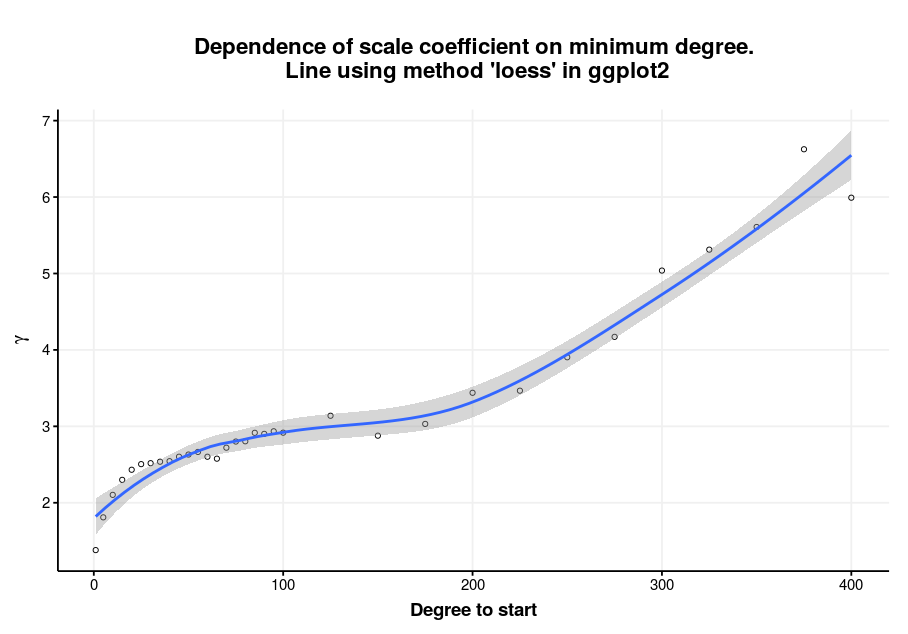
\includegraphics[width=\textwidth]{images/chapter3/poweRlaw/Rplot_gamma_theme.png}
    \caption[$\gamma$ as function of $x_{min}$]{$\gamma$ as a function of $x_{min}$. }
    \tiny\url{source('~/RProjects/PhD_graphs/calculate_gamma_theme.R')}
    \label{fig:gamma_main}
\end{figure}

\section{===Removed===}

\subsection{Introduction to this chapter}




Although network science is a new discipline, it has been the subject of detailed popular science books \cite{barabasi2002linked} and one of its principles\footnote{the small world property} has been the subject of a play\cite{guare1990six},film and parlour game \footnote{Six Degrees of Kevin Bacon}\cite{collins1998s}. Many educated persons would \textit{now} be able to give an accurate answer to Milgram's question. 

 Hindsight bias \cite{fischhoff1975hindsight},\cite{fischhoff2007early}, the phenomenon where the probability of an event or finding seems greater after it has occurred, can make these results seem trivial because one can find plausible explanations for an effect or lack of effect from gene centrality on diseases and traits in general and for any specific entity. If one knew the association between centrality measures and intelligence, or any other complex trait, one could construct a convincing argument that this finding is to be expected. However the specific effect of proteins' position in the synaptic proteome network on synaptic function and complex traits remain unknown. Even if they were established for one trait it is not the case that they would hold for all. Even effects believed to be well established on simple model organisms, such as yeast, are more complicated that they first appeared as will be discussed in section~\ref{sec:Degree and essentialness}. The approach to assessing the role of central genes and gene products for a disorder or trait must therefore be both empirical and make use of the most accurate data we have to date. 
 
 A variety of biological networks exist and the significance of their topologies may differ. The existing literature on network centrality measures in molecular biology include both \todo{rephrase} gene regulatory networks and protein-protein interaction networks. Network analyses of gene function and regulation are often carried out upon co-expression networks, where an edge occurs when the expression of two genes are correlated\cite{zhang2005general}. The implications of modular structure or centrality can, therefore, be different from a protein protein interaction network. A hub node is co-expressed with a variety of different genes and may represent a driver of a biological process such as a transcriptional regulator \cite{parikshak2015systems}.
%  \todo{ DONE cite parikshak}
\todo{or footnote they have to be proximate in protein protein interaction networks}
 A hub node in a protein-protein interaction network has promiscuous interaction partners but may not drive a single process but be essential to several different processes\cite{patil2010hub}\footnote{p1931}. In addition it may interact with different proteins in different sites\cite{han2004evidence}\footnote{party and date hubs}.
 
% \textcolor{green}{? remove  this bitor move to earlier bit}While the measures of vertex importance are precisely defined how they will map onto animal models or complex traits is not and one can construct several plausible hypotheses of effect, effect of specific measures or no effect (hence the quotation at the start of the chapter\todo{?move this down into a fuller introduction section}.
\subsection{Goals of this chapter}

In this section I will test the hypothesis that genes with genetic variants associated with differences in educational attainment and intelligence are more likely to be central in the synaptic proteome network.

I will also test the properties the PSP has at a network level that may impact its function. I will test to see whether the degree distribution is scale free, whether the network has a small world configuration and whether its nodes are more likely to link together if they share certain properties (assortativity), and the implications this may have for its formation. 

I will calculate measures of the centrality or importance of individual nodes and test to see if these important nodes share common properties, support the centrality lethality hypothesis, and are disproportionately involved in animal models of cognition, in addition to determining if these genes are more significant in the samples of intelligence and educational attainment. I will determine if there is evidence to support that genes associated with intelligence are evolutionarily preserved using both gene list methods and population scale genomic data, and whether this is more or less true of synaptic genes. I will also use literature databases and genomic data to test whether central nodes are under purifying selection pressure. Finally I will determine whether animal model of cognition genes and genes found in human studies are more likely to form cohesive groups in the network consistent with the disease module hypothesis. 

In order to introduce these methods and results I will need to explain the main network statistics and centrality measures, explain what is known of the effects of central nodes in networks and in biology, introduce the concept of centrality lethality and of disease modules. 
\subsection{C(k)}
\begin{equation}
    log(C(k) = log(b) - \beta log(k).
\end{equation}


 in figure~\ref{tab:log_linear_model_c_k}
 
 
 \subsubsection{Q SUPPPLEMENTAL Linear model}
 A linear model of the log10 transformation of $C(k)$ and $k$, $log10(C(k))$ and $log10(k)$ is

\begin{equation}
C(k) = 10^{a + m \textrm{log}_{10}(k)},
\end{equation}
if $a$ and $m$ are the coefficients of the linear model or

\begin{equation}
    C(k) = 10^a k^m.
\end{equation}

Matching terms with equation~\ref{eq:C(k) function average transitivity and degree}

\begin{equation}
    C(k) = 10^a k^m = B k^{-\beta},
\end{equation}

so $B=10^a$ and $\beta=-m$ and fitting a linear model of the log transformed variables in and then transforming back the variables R is $B=0.604$ and $\beta$ = 0.453 (table~\ref{tab:log_linear_model_c_k} for coefficients of log10 model).


% Table created by stargazer v.5.2.2 by Marek Hlavac, Harvard University. E-mail: hlavac at fas.harvard.edu
% Date and time: Wed, Mar 10, 2021 - 17:01:23
\begin{table}[!htbp] \centering 
  
\begin{tabular}{@{\extracolsep{5pt}}lc} 
\\[-1.8ex]\hline 
\hline \\[-1.8ex] 
 & \multicolumn{1}{c}{\textit{Dependent variable:}} \\ 
\cline{2-2} 
\\[-1.8ex] & log10($C(k)$) \\ 
\hline \\[-1.8ex] 
 log10 Degree & $-$0.454$^{***}$ \\ 
  & (0.035) \\ 
  & \\ 
 Constant & $-$0.219$^{***}$ \\ 
  & (0.066) \\ 
  & \\ 
\hline \\[-1.8ex] 
Observations & 150 \\ 
R$^{2}$ & 0.533 \\ 
Adjusted R$^{2}$ & 0.530 \\ 
Residual Std. Error & 0.192 (df = 148) \\ 
F Statistic & 169.020$^{***}$ (df = 1; 148) \\ 
\hline 
\hline \\[-1.8ex] 
\textit{Note:}  & \multicolumn{1}{r}{$^{*}$p$<$0.1; $^{**}$p$<$0.05; $^{***}$p$<$0.01} \\ 
\end{tabular} 
\caption{Linear model of the effect of degree $k$ on log $C(k)$\url{source('~/RProjects/chapter3/R/transitivity/transitivity_and_degree/stargazer_cleaner.R')}} 
  \label{tab:log_linear_model_c_k} 
\end{table} 


\todo{fit non transformed linear model}
\textcolor{red}{plot the parameters with the empirical data}
Fitting a linear model omitting degree 1 and with log10 degree has Adjusted R-squared 0.61 compared to 0.4594 for the non logarithmic model.

\footnote{remove\textcolor{red}{Actually the first three points have high leverage for this perhaps should try the powerlaw x min but is not a distribution}

R sq 0.65 going from degree 5 so not too much different}


\begin{figure}
    \centering
    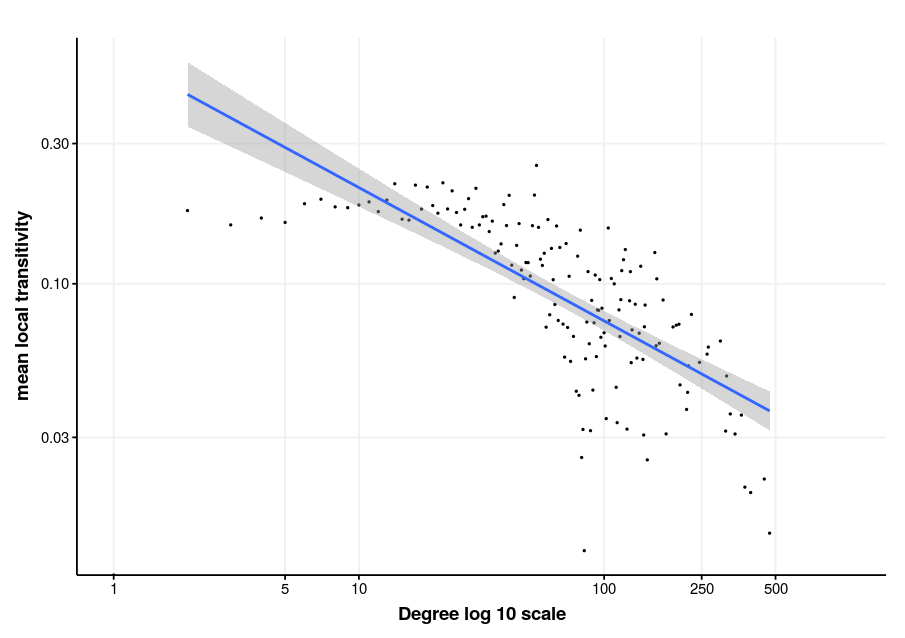
\includegraphics[width=\textwidth]{images/chapter3/ggplot2/c(k)/Rplot_C_k_new_formatted.png}
    \caption[Log10 plot of $C(k)$ against $k$]{Plot of degree $k$ log 10 scale with $C(k)$ also log 10 scale where $C(k)$ is the mean local undirected transitivity at degree $k$. Dark blue line represents line of linear regression and grey shading 95\% confidence intervals. The plot appears to bend down above approximately $k=50$. \url{source('~/RProjects/chapter3/R/transitivity/transitivity_and_degree/mean_deg_seq.R')}}
    \label{fig:C(k)_doublelog}
\end{figure}

\subsubsection{Minimum degree and correlation with transitivity}

Like the coefficient of the power law the correlation coefficient between transitivity and degree depends on the minimum value of transitivity used and varies as a function of $C_{i min}$ and the way in which isolates have been treated.

The degree is not normally distributed so we have calculated Spearman's rank correlation. 


\subsection{results small world}

\paragraph{Global transitivity}


The expected value of the global clustering coefficient with a given degree distribution connected randomly \cite{newman2018networks}\footnote{p332} is:

\begin{equation}
    C=\frac{1}{n}\frac{[<k^2> - <k>]^2}{<k^3>}
\end{equation}


The value of this for the PSP is 0.004541763 compared to the simulated value of 0.00510. \footnote{code \url{source('~/RProjects/centrality/R/transitivity/Expected_global_transitivity.R')}}. The global clustering coefficient is therefore high. Newman states p334 \cite{newman2018networks} that it is not clear why certain non social networks have higher than expected global clustering (for social networks it is ascribed to social choice). For other networks such as the internet with very right skewed degree distribution the clustering coefficient is less than expected. For biological systems such as food webs or the world wide web it is hypothesised that this may due to community formation (\cite{newman2018networks}\footnote{p36})


\paragraph{Feb}
Walkthrough of the global transitivities at \url{/home/grant/RProjects/chapter3/R/transitivity/global_transitivity/mkdown/global_transitivity_markdown.Rmd}




\subsubsection{Local clustering coefficient Results}
Local clustering coefficient tends to be inversely proportional to degree. It is undefined for nodes of degree one. See~figure \ref{fig:log_transitivity_degree}. It is suggested that this may also be due to community formation \cite{newman2018networks} p335.

Mean local transitivity is 0.171 (table~\ref{tab:Different global transitivities in igraph}). The distribution is right skewed with median of 0.129 and 3rd quartile of 0.23 and first quartile of 0.043. This does not match the arithmetic mean of vertex local clustering below it may be down to how we deal with NA. Above calculated as NA.rm
\subsubsection{Average path length}
Average path length for an Erdos Renyi graph on 1000 iterations (type gnm) 3.118 sd 0.00048

Mean global transitivity PSP Watts and Strogatz, isolates to 0 = 0.156. If setting isolates to NA and removing NA = 0.1713.

ER Mean global transititivity (Watts and Strogatz, isolates to 0) 0.0051

ER mean global transitivity (Watts and strogatz, isolates NA and remove 0.0051 (not identical isolates to 0 0.005098806, na 0.005116117)

ER mean global transitivity (triangles 0.005100209 \todo{change to correct sf but keep for now for check not using equal values}) sd 0.0001625842

% latex table generated in R 3.6.3 by xtable 1.8-4 package
% Sat Jun 20 16:17:24 2020
\begin{table}[ht]
\centering
\begin{tabular}{rlrrr}
  \hline
 & variable & mean & sd & PSP \\ 
  \hline
1 & mean\_dist & 3.1182075093 & 0.0004731233 & 2.9797920751 \\ 
  2 & global\_transitivity & 0.0051154572 & 0.0001546763 & 0.0697271768 \\ 
  3 & global\_transitivity\_ws & 0.0051243477 & 0.0001684787 & 0.1562997932 \\ 
  4 & global\_transitivity\_wsNA & 0.0051243477 & 0.0001684787 & 0.1713696115 \\ 
   \hline
\end{tabular}
\caption{Supplemental 10 sf to show that the values are not identical Erdos renyi n3457 m 30498 graph. \textcolor{red}{check and to supplemental}}
\label{tab:transitivity_erdos_renyi 10sf}
\end{table}
% latex table generated in R 3.6.3 by xtable 1.8-4 package
% Sat Jun 20 16:07:46 2020

% latex table generated in R 3.6.3 by xtable 1.8-4 package
% Sat Jun 20 16:19:29 2020
\begin{table}[ht]
\centering
\begin{tabular}{rlrrr}
  \hline
 & variable & mean & sd & PSP \\ 
  \hline
1 & mean\_dist & 3.1182 & 0.0005 & 2.9798 \\ 
  2 & global\_transitivity & 0.0051 & 0.0002 & 0.0697 \\ 
  3 & global\_transitivity\_ws & 0.0051 & 0.0002 & 0.1563 \\ 
  4 & global\_transitivity\_wsNA & 0.0051 & 0.0002 & 0.1714 \\ 
   \hline
\end{tabular}
\caption{Erdos renyi n3457 m 30498 graph. \textcolor{red}{? add difference mean and PSP to compare to sd. ? add watts strogatz 0 to show difference with na and then add in table caption. WS and global are almost identical in random model. Cross ref to Estrada :pca; and Global clustering. WS is higher in most real world networks where it diverges}}
\label{tab:transitivity_erdos_renyi}
\end{table}

See table~\ref{tab:transitivity_erdos_renyi}\footnote{Code \url{source('~/RProjects/graph_sw/R/small_world_random/er_random_ws.R')}}




% Sat Jun 20 16:38:56 2020
\begin{table}[ht]
\centering
\begin{tabular}{rlrrr}
  \hline
 & variable & $\mu\textsubscript{random}$ & $s.d.\textsubscript{random}$ & PSP \\ 
  \hline
1 & Average path length & \textbf{3.0069} & 0.0053 & 2.9798 \\ 
  2 & Global transitivity $C$ & 0.0584 & 0.0008 & 0.0697 \\ 
  3 & Global transitivity WS $C_{WS}$ &\textbf{ 0.0683} & 0.0019 & 0.1563 \\ 
  4 & global transitivity WS NA $C_{WSNA}$ & 0.0748 & 0.0020 & 0.1714 \\ 
   \hline
\end{tabular}
\caption{Degree corrected configuration model transitivity and average path length. The average path length is smaller than in the Erdos Renyi model likely due to the increased number of hubs. \textcolor{red}{WS $>$ global for real world networks per Estrada. Shorter APL per Albert (than Erdos Renyi} See small world scale free networks are ultra small. \textcolor{red}{Add mu - sd}}
\label{tab:cmtransitivity_configuration_model}
\end{table}


% Sat Jun 20 16:38:56 2020
\begin{table}[ht]
\centering
\begin{tabular}{rlrrr}
  \hline
 & variable & $\mu\textsubscript{random}$ & $s.d.\textsubscript{random}$ & PSP \\ 
  \hline
1 & Average path length & \textbf{3.0069} & 0.0053 & 2.9798 \\ 
  2 & Global transitivity $C$ & 0.0584 & 0.0008 & 0.0697 \\ 
  3 & Global transitivity WS $C_{WS}$ &\textbf{ 0.0683} & 0.0019 & 0.1563 \\ 
  4 & global transitivity WS NA $C_{WSNA}$ & 0.0748 & 0.0020 & 0.1714 \\ 
   \hline
\end{tabular}
\caption{Degree corrected configuration model transitivity and average path length. The average path length is smaller than in the Erdos Renyi model likely due to the increased number of hubs. \textcolor{red}{WS $>$ global for real world networks per Estrada. Shorter APL per Albert (than Erdos Renyi} See small world scale free networks are ultra small. \textcolor{red}{Add mu - sd}}
\label{tab:cmtransitivity_configuration_model}
\end{table}

% \begin{figure}
%     \centering
%     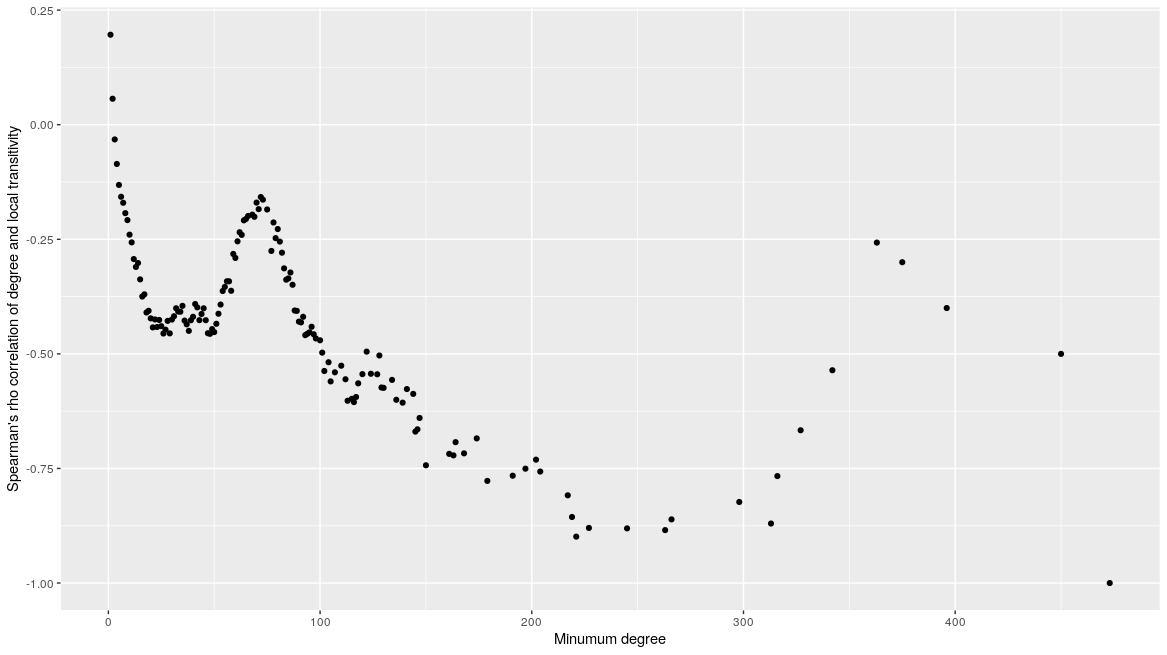
\includegraphics[width=\textwidth]{images/Rplot01_min_degree_transitivity.png}
%     \caption{Plot of minumum degree included in the calculation of Spearmans rank correlation between degree and $\rho$. Although the overall coefficient is positive the correlation for nodes above degree 5 are clearly negative and this becomes more apparent at high degree. This relationship is therefore complex and the typical relationship described in the literature may only hold for the large networks in which this relationship has been studies such as the internet. Potential replacement \url{source('~/RProjects/chapter3/R/transitivity/transitivity_and_degree/mean_deg_seq.R')} plot q}
%     \label{fig:Plot of minumum degree included in the calculation of Spearmans rank correlation between degree and rho}
% \end{figure}
% \textcolor{red}{moved from earlier to be towards small world}

\paragraph{Second bit APL}

\subsubsection{Comparison with erdos renyi graph}
"In the post synaptic proteome average path length is 2.979792. Global transitivity (Newman) is 0.069727 and transitivityWS is 0.171370(NA)"\textcolor{red}{WS$>>$ than global see p254 fig3a Estrada}

Watts strogatz transitivity with isolates to zero and isolates to NA and excluded is as below
"Transitivity zero 0.156300\textcolor{red}{this is the actual WS as described ie average and isolates to zero)}   Transitivity NA 0.171370"

The igraph function transitivity with type option "localaverageundirected" yields transitivityNA ie the absolute difference it 1000 iterations is less than $1\times10^{-15}$.

% latex table generated in R 3.6.3 by xtable 1.8-4 package
% Tue Oct 27 16:53:10 2020
\begin{table}[ht]
\centering
\begin{tabular}{lrrrrlll}
  \hline
name & mean & sd & d & pKS & Z &CI & ?\% CI  \\ 
  \hline
average path length & 3.11797 (2.979) & 0.00049 & 0.019 & 0.84 & 8907 &  3.117939& 3.118000 \\ 
  transitivity WS & 0.00510 (0.171) & 0.00017 & 0.015 & 0.98 &  -30452 & 0.005089474 &0.005110830 \\ 
  transitivityNA & 0.00510 & 0.00017 & 0.015 & 0.98 \\ 
  transitivity0 & 0.00510 & 0.00017 & 0.015 & 0.98 \\ 
  globaltransitivity & 0.00510 (0.0697) & 0.00017 & 0.014 & 0.99 \\ 
   \hline
\end{tabular}
\caption{Mean transitivity values for 1000 iterations of Erdos Renyi gnp model. Kolmogorov Smirnov statistic D = distance p = pvalue. One-sample Kolmogorov Smirnov test for normality. alterantive hypothesis two sided. Network values are in parenthesis. Using package BSDA alternative hypothesis true mean is not equal to PSP value. Note transitivity results are not identical other than transitivityWS and NA but are to 3 s.f. p Z $2.2<\times10^{-16}$ \url{source('~/RProjects/chapter3/R/small_world/ks_tests_er_sim.R')} } 
\label{tab:Mean transitivity values for 1000 iterations of Erdos Renyi gnp model.}
\end{table}

If we simulate mean distance using a degree sequence model we find no shorter average path length than found in the PSP (2.9 8) in 1000 iterations.


\subsection{Redo of Small world average path length}

In the small world region the path length is small comparable  or smaller than a random graph but with a high clustering coefficient which would not be seen in a random graph. 




\subsubsection{Comparison with configuration model}
% latex table generated in R 3.6.3 by xtable 1.8-4 package
% Sat Oct 31 14:30:26 2020
\begin{table}[ht]
\centering
\begin{tabular}{lrrrrrr}
  \hline
name & mean & sd & 2.5\% CI & 97.5\% CI & d & p \\ 
  \hline
average path length & 3.007 (2.979) & 0.005 & 2.996 & 3.018 & 0.01 & 0.98 \\ 
  transitivity WS & 0.077 (0.171) & 0.002 & 0.073 & 0.081 & 0.02 & 0.77 \\ 
  transitivityNA & 0.075 & 0.002 & 0.071 & 0.079 & 0.02 & 0.78 \\ 
  transitivity0 & 0.068 & 0.002 & 0.065 & 0.072 & 0.02 & 0.78 \\ 
  globaltransitivity & 0.058 (0.0697) & 0.001 & 0.057 & 0.060 & 0.02 & 0.83 \\ 
   \hline
\end{tabular}
\caption{Mean transitivity values for 1000 iterations of Configuration  model. Kolmogorov Smirnov statistic D = distance p = pvalue. One-sample Kolmogorov Smirnov test for normality. alterantive hypothesis two sided. Confidence interval are for empirical simulations. \url{source('~/RProjects/chapter3/R/small_world/ks_tests_configuration_sim.R')} } 
\label{tab:Mean transitivity values for 1000 iterations of Configuration model.}
\end{table}

\todo{transitivity WS is not equal to NA why?}



\subsubsection{Degree assortativity}
\todo{include the peel multi-scale mixing patterns}
which has similar degree assortativity to that calculated by Newman for the yeast interactome \cite{jeong2001lethality}.
\todo{? move this to discussion} Although it is not clear why this is the case it does have implications for models of how the the PSP was generated (including gene duplication and ortholog degree) and for 


consistent with older nodes being connected to each other and hence in turn being more likely to be connected to others which would be accurate for














































\section{Supplemental Gene Ontology Enrichment}
\subsection{Betweenness ToppGene}
\subsubsection{High betweenness}
\paragraph{Molecular function}
Molecular function see table~\ref{tab:ToppGENE GO: Molecular Function. bet 90 centile cwpsp.txtp = p value; q FDR B H = q adjusted significance level False Discovery Rate using Benjamini and Hochberg adjustment; n= n genes annotated in test group; n PSP= n genes annotated in PSP}


% latex table generated in R 3.6.3 by xtable 1.8-4 package
% Sun Oct  4 11:46:04 2020
\begin{table}[ht]
\centering
\begin{adjustbox}{width=\textwidth}
\setlength{\extrarowheight}{2pt}
\begin{tabular}{@{}clllcl@{}}
  \toprule
  ID & Molecular Function & $n$ & $n$ PSP & $p$ & $q$ FDR B H \\ 

  \midrule
GO:0044877 & protein-containing complex binding & 120 & 513 & $1.74 \times 10^{-22}$ & $1.83 \times 10^{-19}$ \\ 
  GO:0031625 & ubiquitin protein ligase binding & 51 & 117 & $5.84 \times 10^{-22}$ & $3.07 \times 10^{-19}$ \\ 
  GO:0044389 & ubiquitin-like protein ligase binding & 52 & 123 & $1.24 \times 10^{-21}$ & $4.34 \times 10^{-19}$ \\ 
  GO:0019904 & protein domain specific binding & 89 & 329 & $1.02 \times 10^{-20}$ & $2.69 \times 10^{-18}$ \\ 
  GO:0019900 & kinase binding & 76 & 325 & $9.81 \times 10^{-14}$ & $2.06 \times 10^{-11}$ \\ 
  GO:0008234 & cysteine-type peptidase activity & 54 & 189 & $1.31 \times 10^{-13}$ & $2.29 \times 10^{-11}$ \\ 
  GO:0008134 & transcription factor binding & 48 & 156 & $1.64 \times 10^{-13}$ & $2.45 \times 10^{-11}$ \\ 
  GO:0005102 & signaling receptor binding & 87 & 405 & $2.09 \times 10^{-13}$ & $2.74 \times 10^{-11}$ \\ 
  GO:0050839 & cell adhesion molecule binding & 69 & 288 & $5.05 \times 10^{-13}$ & $5.88 \times 10^{-11}$ \\ 
  GO:0019901 & protein kinase binding & 69 & 295 & $1.77 \times 10^{-12}$ & $1.86 \times 10^{-10}$ \\ 
   \bottomrule
\end{tabular}
\end{adjustbox}
\caption[Gene ontology enrichment High betweenness genes Molecular Function of genes above 90th centile of distribution]{\textbf{High betweenness genes. Cellular Component - Gene ontology enrichment analysis} using the ToppGene web client and all PSP genes as the background set.  Biological process tested gene set is 90th centile of degree distribution.  p value; q FDR B H = q adjusted significance level False Discovery Rate using Benjamini and Hochberg adjustment; $n$= $n$ genes annotated in test group; $n$ PSP= n genes annotated in PSP. $n$ ontology terms significantly (q FDR$>=0.05$) enriched for this centrality measure and ontology category (e.g. MF,CC,BP): \textcolor{red}{n}} 

\label{tab:ToppGENE GO: Molecular Function. bet 90 centile cwpsp.txtp = p value; q FDR B H = q adjusted significance level False Discovery Rate using Benjamini and Hochberg adjustment; n= n genes annotated in test group; n PSP= n genes annotated in PSP}
\end{table}

\paragraph{Biological process}
Biological process table~\ref{tab:ToppGENE GO: Biological Process. bet 90 centile cwpsp.txtp = p value; q FDR B H = q adjusted significance level False Discovery Rate using Benjamini and Hochberg adjustment; n= n genes annotated in test group; n PSP= n genes annotated in PSP}
% latex table generated in R 3.6.3 by xtable 1.8-4 package
% Sun Oct  4 11:49:29 2020
  \begin{table}[ht]
\centering
\begin{adjustbox}{width=\textwidth}
\setlength{\extrarowheight}{2pt}
\begin{tabular}{@{}clllcl@{}}
  \toprule
  ID & Biological Process & $n$ & $n$ PSP & $p$ & $q$ FDR B H \\ 

  \midrule
GO:0007049 & cell cycle & 124 & 489 & $5.10 \times 10^{-27}$ & $3.33 \times 10^{-23}$ \\ 
  GO:0051247 & positive regulation of protein metabolic process & 117 & 463 & $4.11 \times 10^{-25}$ & $1.34 \times 10^{-21}$ \\ 
  GO:0042981 & regulation of apoptotic process & 108 & 416 & $5.38 \times 10^{-24}$ & $1.17 \times 10^{-20}$ \\ 
  GO:0043067 & regulation of programmed cell death & 108 & 423 & $2.44 \times 10^{-23}$ & $3.99 \times 10^{-20}$ \\ 
  GO:0009894 & regulation of catabolic process & 95 & 350 & $2.16 \times 10^{-22}$ & $2.82 \times 10^{-19}$ \\ 
  GO:0006508 & proteolysis & 105 & 417 & $4.31 \times 10^{-22}$ & $4.29 \times 10^{-19}$ \\ 
  GO:0010941 & regulation of cell death & 112 & 464 & $4.60 \times 10^{-22}$ & $4.29 \times 10^{-19}$ \\ 
  GO:0032270 & positive regulation of cellular protein metabolic process & 106 & 433 & $2.89 \times 10^{-21}$ & $2.36 \times 10^{-18}$ \\ 
  GO:0009057 & macromolecule catabolic process & 106 & 443 & $2.02 \times 10^{-20}$ & $1.47 \times 10^{-17}$ \\ 
  GO:0043066 & negative regulation of apoptotic process & 73 & 240 & $3.94 \times 10^{-20}$ & $2.36 \times 10^{-17}$ \\ 
   \bottomrule
\end{tabular}
\end{adjustbox}
\caption[Gene ontology enrichment High betweenness genes Biological Process of genes above 90th centile of distribution]{\textbf{High betweenness genes. Biological Process - Gene ontology enrichment analysis} using the ToppGene web client and all PSP genes as the background set.  Biological process tested gene set is 90th centile of degree distribution.  p value; q FDR B H = q adjusted significance level False Discovery Rate using Benjamini and Hochberg adjustment; $n$= $n$ genes annotated in test group; $n$ PSP= n genes annotated in PSP. $n$ ontology terms significantly (q FDR$>=0.05$) enriched for this centrality measure and ontology category (e.g. MF,CC,BP): \textcolor{red}{n}\url{source('~/RProjects/chapter3/R/sig_magma_genes/central_genes_toppgene/betweenness/5_0_clip_centrality_bet_hig_bp.R')}} 
\label{tab:ToppGENE GO: Biological Process. bet 90 centile cwpsp.txtp = p value; q FDR B H = q adjusted significance level False Discovery Rate using Benjamini and Hochberg adjustment; n= n genes annotated in test group; n PSP= n genes annotated in PSP}
\end{table}

\paragraph{Cellular component}
Cellular component table~\ref{tab:ToppGENE GO: Cellular Component. bet 90 centile cwpsp.txtp = p value; q FDR B H = q adjusted significance level False Discovery Rate using Benjamini and Hochberg adjustment; n= n genes annotated in test group; n PSP= n genes annotated in PSP}
% latex table generated in R 3.6.3 by xtable 1.8-4 package
% Sun Oct  4 11:50:08 2020

    \begin{table}[ht]
\centering
\begin{adjustbox}{width=\textwidth}
\setlength{\extrarowheight}{2pt}
\begin{tabular}{@{}clllcl@{}}
  \toprule
  ID & Cellular Component & $n$ & $n$ PSP & $p$ & $q$ FDR B H \\ 

  \midrule
GO:0015630 & microtubule cytoskeleton & 98 & 447 & $4.56 \times 10^{-16}$ & $4.02 \times 10^{-13}$ \\ 
  GO:0005814 & centriole & 55 & 194 & $7.79 \times 10^{-14}$ & $3.43 \times 10^{-11}$ \\ 
  GO:0005813 & centrosome & 52 & 182 & $2.92 \times 10^{-13}$ & $8.59 \times 10^{-11}$ \\ 
  GO:0005815 & microtubule organizing center & 62 & 246 & $6.14 \times 10^{-13}$ & $1.35 \times 10^{-10}$ \\ 
  GO:0030990 & intraciliary transport particle & 51 & 212 & $5.95 \times 10^{-10}$ & $8.73 \times 10^{-8}$ \\ 
  GO:0005929 & cilium & 51 & 212 & $5.95 \times 10^{-10}$ & $8.73 \times 10^{-8}$ \\ 
  GO:0098589 & membrane region & 42 & 160 & $1.37 \times 10^{-9}$ & $1.72 \times 10^{-7}$ \\ 
  GO:0005819 & spindle & 35 & 120 & $1.74 \times 10^{-9}$ & $1.92 \times 10^{-7}$ \\ 
  GO:0099513 & polymeric cytoskeletal fiber & 87 & 482 & $3.13 \times 10^{-9}$ & $2.46 \times 10^{-7}$ \\ 
  GO:0045121 & membrane raft & 41 & 158 & $3.20 \times 10^{-9}$ & $2.46 \times 10^{-7}$ \\ 
   \hline
\end{tabular}
\end{adjustbox}
\caption[Gene ontology enrichment High betweenness genes Cellular Component of genes above 90th centile of distribution]{\textbf{High betweenness genes. Cellular Component - Gene ontology enrichment analysis} using the ToppGene web client and all PSP genes as the background set.  Biological process tested gene set is 90th centile of degree distribution.  p value; q FDR B H = q adjusted significance level False Discovery Rate using Benjamini and Hochberg adjustment; $n$= $n$ genes annotated in test group; $n$ PSP= n genes annotated in PSP. $n$ ontology terms significantly (q FDR$>=0.05$) enriched for this centrality measure and ontology category (e.g. MF,CC,BP): \textcolor{red}{n}}
\label{tab:ToppGENE GO: Cellular Component. bet 90 centile cwpsp.txtp = p value; q FDR B H = q adjusted significance level False Discovery Rate using Benjamini and Hochberg adjustment; n= n genes annotated in test group; n PSP= n genes annotated in PSP}
\end{table}





\clearpage

\subsubsection{Low betweenness}

\paragraph{Cellular component}

Cellular component table~\ref{tab:ToppGENE GO: Cellular Component. bet 10 centile cwpsp.txtp = p value; q FDR B H = q adjusted significance level False Discovery Rate using Benjamini and Hochberg adjustment; n= n genes annotated in test group; n PSP= n genes annotated in PSP}


% latex table generated in R 3.6.3 by xtable 1.8-4 package
% Sun Oct  4 11:58:29 2020
\begin{table}[ht]
\centering
\begin{adjustbox}{width=\textwidth}
\setlength{\extrarowheight}{2pt}
\begin{tabular}{@{}clllcl@{}}
  \toprule
  ID & Cellular Component & $n$ & $n$ PSP & $p$ & $q$ FDR B H \\ 

  \midrule
GO:0031226 & intrinsic component of plasma membrane & 61 & 331 & $1.85 \times 10^{-6}$ & $9.76 \times 10^{-4}$ \\ 
  GO:0005887 & integral component of plasma membrane & 56 & 307 & $7.36 \times 10^{-6}$ & $1.94 \times 10^{-3}$ \\ 
   \bottomrule
\end{tabular}
\end{adjustbox}
\caption[Gene ontology enrichment Low betweenness genes Cellular Component of genes below 10th centile of distribution]{\textbf{Low betweenness genes. Cellular Component - Gene ontology enrichment analysis} using the ToppGene web client and all PSP genes as the background set.  Biological process tested gene set is below 10th centile of degree distribution.  p value; q FDR B H = q adjusted significance level False Discovery Rate using Benjamini and Hochberg adjustment; $n$= $n$ genes annotated in test group; $n$ PSP= n genes annotated in PSP. $n$ ontology terms significantly (q FDR$>=0.05$) enriched for this centrality measure and ontology category (e.g. MF,CC,BP): \textcolor{red}{n}}
\label{tab:ToppGENE GO: Cellular Component. bet 10 centile cwpsp.txtp = p value; q FDR B H = q adjusted significance level False Discovery Rate using Benjamini and Hochberg adjustment; n= n genes annotated in test group; n PSP= n genes annotated in PSP}
\end{table}

\paragraph{Pathway}

Extra cellular matrix table~\ref{tab:ToppGENE Pathway. bet 10 centile cwpsp.txtp = p value; q FDR B H = q adjusted significance level False Discovery Rate using Benjamini and Hochberg adjustment; n= n genes annotated in test group; n PSP= n genes annotated in PSP}. Glycosylphosphatidylinositol proteins (GPI proteins) are directed to the endoplasmic reticulum. 




% latex table generated in R 3.6.3 by xtable 1.8-4 package
% Sun Oct  4 12:01:20 2020
\begin{table}[ht]
\centering
\begin{adjustbox}{width=\textwidth}
\begin{tabular}{lcllcl}
  \hline
ID & Pathway & n & n PSP & p & q FDR B H \\ 
  \hline
M5889 &\makecell{ Ensemble of genes encoding extracellular matrix\\ and extracellular matrix-associated proteins}  & 21 & 91 & $7.23 \times 10^{-6}$ & $8.28 \times 10^{-3}$ \\ 
  M1268710 & \makecell{Post-translational modification: synthesis of GPI-anchored proteins} & 6 & 11 & $9.13 \times 10^{-5}$ & $4.00 \times 10^{-2}$ \\ 
  M5884 & \makecell{Ensemble of genes encoding core extracellular matrix including\\ ECM glycoproteins, collagens and proteoglycans} & 10 & 31 & $1.05 \times 10^{-4}$ & $4.00 \times 10^{-2}$ \\ 
   \hline
\end{tabular}
\end{adjustbox}
\caption{ToppGene Pathway. bet 10 centile cwpsp.txtp = p value; q FDR B H = q adjusted significance level False Discovery Rate using Benjamini and Hochberg adjustment; n= n genes annotated in test group; n PSP= n genes annotated in PSP} 
\label{tab:ToppGENE Pathway. bet 10 centile cwpsp.txtp = p value; q FDR B H = q adjusted significance level False Discovery Rate using Benjamini and Hochberg adjustment; n= n genes annotated in test group; n PSP= n genes annotated in PSP}
\end{table}

\clearpage
\subsection{Closeness Centrality ToppGene}



\paragraph{Molecular function}

Molecular function Gene Ontology Enrichment High Closeness centrality in table \ref{tab:ToppGENE GO: Molecular Function. clo 90 centile cwpsp.txtp = p value; q FDR B H = q adjusted significance level False Discovery Rate using Benjamini and Hochberg adjustment; n= n genes annotated in test group; n PSP= n genes annotated in PSP}

% latex table generated in R 3.6.3 by xtable 1.8-4 package
% Sun Oct  4 12:10:43 2020

  \begin{table}[ht]
\centering
\begin{adjustbox}{width=\textwidth}
\setlength{\extrarowheight}{2pt}
\begin{tabular}{@{}clllcl@{}}
  \toprule
  ID & Molecular Function & $n$ & $n$ PSP & $p$ & $q$ FDR B H \\ 

  \midrule
GO:0003723 & RNA binding & 167 & 554 & $2.11 \times 10^{-50}$ & $2.14 \times 10^{-47}$ \\ 
  GO:0031625 & ubiquitin protein ligase binding & 57 & 117 & $1.38 \times 10^{-27}$ & $7.00 \times 10^{-25}$ \\ 
  GO:0044389 & ubiquitin-like protein ligase binding & 58 & 123 & $4.10 \times 10^{-27}$ & $1.39 \times 10^{-24}$ \\ 
  GO:0051082 & unfolded protein binding & 31 & 56 & $2.20 \times 10^{-17}$ & $5.57 \times 10^{-15}$ \\ 
  GO:0044877 & protein-containing complex binding & 110 & 513 & $4.36 \times 10^{-17}$ & $8.84 \times 10^{-15}$ \\ 
  GO:0019904 & protein domain specific binding & 81 & 329 & $5.59 \times 10^{-16}$ & $9.46 \times 10^{-14}$ \\ 
  GO:0003729 & mRNA binding & 39 & 100 & $6.55 \times 10^{-15}$ & $9.50 \times 10^{-13}$ \\ 
  GO:0008134 & transcription factor binding & 50 & 156 & $8.56 \times 10^{-15}$ & $1.09 \times 10^{-12}$ \\ 
  GO:0005102 & signaling receptor binding & 86 & 405 & $7.31 \times 10^{-13}$ & $8.25 \times 10^{-11}$ \\ 
  GO:0140097 & catalytic activity, acting on DNA & 31 & 76 & $1.13 \times 10^{-12}$ & $1.15 \times 10^{-10}$ \\ 
   \bottomrule
\end{tabular}
\end{adjustbox}
\caption[Gene ontology enrichment High Closeness genes Molecular Function of genes above 90th centile of distribution]{\textbf{High Closeness genes. Molecular Function - Gene ontology enrichment analysis} using the ToppGene web client and all PSP genes as the background set.  Molecular function tested gene set is 90th centile of degree distribution.  p value; q FDR B H = q adjusted significance level False Discovery Rate using Benjamini and Hochberg adjustment; $n$= $n$ genes annotated in test group; $n$ PSP= n genes annotated in PSP. $n$ ontology terms significantly (q FDR$>=0.05$) enriched for this centrality measure and ontology category (e.g. MF,CC,BP): \textcolor{red}{n}} 
\label{tab:ToppGENE GO: Molecular Function. clo 90 centile cwpsp.txtp = p value; q FDR B H = q adjusted significance level False Discovery Rate using Benjamini and Hochberg adjustment; n= n genes annotated in test group; n PSP= n genes annotated in PSP}
\end{table}

\paragraph{Biological Process}
Biological process table~\ref{tab:ToppGENE GO: Biological Process. clo 90 centile cwpsp.txtp = p value; q FDR B H = q adjusted significance level False Discovery Rate using Benjamini and Hochberg adjustment; n= n genes annotated in test group; n PSP= n genes annotated in PSP}

% latex table generated in R 3.6.3 by xtable 1.8-4 package
% Sun Oct  4 12:13:59 2020
\begin{table}[ht]
\centering
\begin{adjustbox}{width=\textwidth}
\setlength{\extrarowheight}{2pt}
\begin{tabular}{@{}clllcl@{}}
  \toprule
  ID & Biological Process & $n$ & $n$ PSP & $p$ & $q$ FDR B H \\ 

  \midrule
GO:0044265 & cellular macromolecule catabolic process & 131 & 372 & $4.77 \times 10^{-46}$ & $2.98 \times 10^{-42}$ \\ 
  GO:0009057 & macromolecule catabolic process & 143 & 443 & $1.34 \times 10^{-45}$ & $4.18 \times 10^{-42}$ \\ 
  GO:0016071 & mRNA metabolic process & 106 & 260 & $2.87 \times 10^{-43}$ & $5.96 \times 10^{-40}$ \\ 
  GO:0044403 & symbiotic process & 125 & 364 & $3.12 \times 10^{-42}$ & $4.86 \times 10^{-39}$ \\ 
  GO:0044419 & interspecies interaction between organisms & 125 & 368 & $1.23 \times 10^{-41}$ & $1.53 \times 10^{-38}$ \\ 
  GO:0016032 & viral process & 118 & 348 & $6.85 \times 10^{-39}$ & $7.13 \times 10^{-36}$ \\ 
  GO:0006402 & mRNA catabolic process & 75 & 180 & $1.13 \times 10^{-30}$ & $1.00 \times 10^{-27}$ \\ 
  GO:0006401 & RNA catabolic process & 76 & 186 & $2.10 \times 10^{-30}$ & $1.63 \times 10^{-27}$ \\ 
  GO:0010608 & posttranscriptional regulation of gene expression & 82 & 225 & $1.11 \times 10^{-28}$ & $7.69 \times 10^{-26}$ \\ 
  GO:0034655 & nucleobase-containing compound catabolic process & 80 & 217 & $2.37 \times 10^{-28}$ & $1.48 \times 10^{-25}$ \\ 
   \bottomrule
\end{tabular}
\end{adjustbox}
\caption[Gene ontology enrichment High Closeness genes Biological Process of genes above 90th centile of distribution]{\textbf{High Closeness genes. Biological Process - Gene ontology enrichment analysis} using the ToppGene web client and all PSP genes as the background set.  Biological process tested gene set is 90th centile of degree distribution.  p value; q FDR B H = q adjusted significance level False Discovery Rate using Benjamini and Hochberg adjustment; $n$= $n$ genes annotated in test group; $n$ PSP= n genes annotated in PSP. $n$ ontology terms significantly (q FDR$>=0.05$) enriched for this centrality measure and ontology category (e.g. MF,CC,BP): \textcolor{red}{n}} 

\label{tab:ToppGENE GO: Biological Process. clo 90 centile cwpsp.txtp = p value; q FDR B H = q adjusted significance level False Discovery Rate using Benjamini and Hochberg adjustment; n= n genes annotated in test group; n PSP= n genes annotated in PSP}
\end{table}





\paragraph{Cellular component}
Cellular component table~\ref{tab:ToppGENE GO: Cellular Component. clo 90 centile cwpsp.txtp = p value; q FDR B H = q adjusted significance level False Discovery Rate using Benjamini and Hochberg adjustment; n= n genes annotated in test group; n PSP= n genes annotated in PSP}

% latex table generated in R 3.6.3 by xtable 1.8-4 package
% Sun Oct  4 12:15:50 2020
\begin{table}[ht]
\centering
\begin{adjustbox}{width=\textwidth}
\setlength{\extrarowheight}{2pt}
\begin{tabular}{@{}clllcl@{}}
  \toprule
  ID & Cellular Component & $n$ & $n$ PSP & $p$ & $q$ FDR B H \\ 

  \midrule
GO:1990904 & ribonucleoprotein complex & 102 & 303 & $5.76 \times 10^{-33}$ & $4.89 \times 10^{-30}$ \\ 
  GO:0005925 & focal adhesion & 77 & 239 & $4.94 \times 10^{-23}$ & $2.10 \times 10^{-20}$ \\ 
  GO:0030055 & cell-substrate junction & 77 & 244 & $2.18 \times 10^{-22}$ & $6.15 \times 10^{-20}$ \\ 
  GO:0005912 & adherens junction & 85 & 314 & $8.51 \times 10^{-20}$ & $1.80 \times 10^{-17}$ \\ 
  GO:0070161 & anchoring junction & 85 & 319 & $2.64 \times 10^{-19}$ & $4.47 \times 10^{-17}$ \\ 
  GO:0035770 & ribonucleoprotein granule & 36 & 78 & $1.03 \times 10^{-16}$ & $1.30 \times 10^{-14}$ \\ 
  GO:0036464 & cytoplasmic ribonucleoprotein granule & 35 & 74 & $1.07 \times 10^{-16}$ & $1.30 \times 10^{-14}$ \\ 
  GO:0000974 & Prp19 complex & 20 & 31 & $2.08 \times 10^{-13}$ & $2.21 \times 10^{-11}$ \\ 
  GO:0101031 & chaperone complex & 16 & 21 & $1.04 \times 10^{-12}$ & $9.79 \times 10^{-11}$ \\ 
  GO:0005681 & spliceosomal complex & 22 & 40 & $1.30 \times 10^{-12}$ & $1.11 \times 10^{-10}$ \\ 
   \bottomrule
\end{tabular}
\end{adjustbox}
\caption[Gene ontology enrichment High Closeness genes Cellular Component of genes above 90th centile of distribution]{\textbf{High Closeness genes. Cellular Component - Gene ontology enrichment analysis} using the ToppGene web client and all PSP genes as the background set.  Biological process tested gene set is 90th centile of degree distribution.  p value; q FDR B H = q adjusted significance level False Discovery Rate using Benjamini and Hochberg adjustment; $n$= $n$ genes annotated in test group; $n$ PSP= n genes annotated in PSP. $n$ ontology terms significantly (q FDR$>=0.05$) enriched for this centrality measure and ontology category (e.g. MF,CC,BP): \textcolor{red}{n}} 

\label{tab:ToppGENE GO: Cellular Component. clo 90 centile cwpsp.txtp = p value; q FDR B H = q adjusted significance level False Discovery Rate using Benjamini and Hochberg adjustment; n= n genes annotated in test group; n PSP= n genes annotated in PSP}
\end{table}






\subsubsection{Low closeness}

Note human phenotype epilepsy and disease enriched\footnote{\url{source('~/RProjects/chapter3/R/sig_magma_genes/central_genes_toppgene/closeness/low_closeness/5_0_clip_centrality_clo_low_cc_n_10.R'}}
\paragraph{Molecular function}
Molecular function table~\ref{tab:ToppGENE GO: Molecular Function. clo 10 centile cwpsp.txtp = p value; q FDR B H = q adjusted significance level False Discovery Rate using Benjamini and Hochberg adjustment; n= n genes annotated in test group; n PSP= n genes annotated in PSP}. Closeness is more normally distributed it appears the low part of its distribution is also more discriminating than those with power law distribution that have a number of genes separated by small absolute values at the lower end of the distribution. Genes encoding proteins with low closeness centrality are enriched for molecular functions involving ion channels and trans-membrane transporters. 

% latex table generated in R 3.6.3 by xtable 1.8-4 package
% Sun Oct  4 12:19:53 2020

  \begin{table}[ht]
\centering
\begin{adjustbox}{width=\textwidth}
\setlength{\extrarowheight}{2pt}
\begin{tabular}{@{}clllcl@{}}
  \toprule
  ID & Molecular Function & $n$ & $n$ PSP & $p$ & $q$ FDR B H \\ 

  \midrule
GO:0005215 & transporter activity & 66 & 419 & $2.40 \times 10^{-5}$ & $1.02 \times 10^{-2}$ \\ 
  GO:0022857 & transmembrane transporter activity & 61 & 378 & $2.44 \times 10^{-5}$ & $1.02 \times 10^{-2}$ \\ 
  GO:0004930 & G protein-coupled receptor activity & 10 & 24 & $3.91 \times 10^{-5}$ & $1.09 \times 10^{-2}$ \\ 
  GO:0043176 & amine binding & 4 & 4 & $1.01 \times 10^{-4}$ & $2.10 \times 10^{-2}$ \\ 
  GO:0046873 & metal ion transmembrane transporter activity & 36 & 203 & $2.12 \times 10^{-4}$ & $3.19 \times 10^{-2}$ \\ 
  GO:0015075 & ion transmembrane transporter activity & 53 & 340 & $2.34 \times 10^{-4}$ & $3.19 \times 10^{-2}$ \\ 
  GO:0022803 & passive transmembrane transporter activity & 39 & 230 & $3.05 \times 10^{-4}$ & $3.19 \times 10^{-2}$ \\ 
  GO:0015267 & channel activity & 39 & 230 & $3.05 \times 10^{-4}$ & $3.19 \times 10^{-2}$ \\ 
  GO:0008324 & cation transmembrane transporter activity & 46 & 288 & $3.61 \times 10^{-4}$ & $3.36 \times 10^{-2}$ \\ 
  GO:0015318 & inorganic molecular entity transmembrane transporter activity & 50 & 324 & $4.60 \times 10^{-4}$ & $3.86 \times 10^{-2}$ \\ 
   \bottomrule
\end{tabular}
\end{adjustbox}
\caption[Gene ontology enrichment Low Closeness genes Molecular Function of genes above 90th centile of distribution]{\textbf{Low Closeness genes. Molecular Function - Gene ontology enrichment analysis} using the ToppGene web client and all PSP genes as the background set.  Biological process tested gene set is below 10th centile of degree distribution.  p value; q FDR B H = q adjusted significance level False Discovery Rate using Benjamini and Hochberg adjustment; $n$= $n$ genes annotated in test group; $n$ PSP= n genes annotated in PSP. $n$ ontology terms significantly (q FDR$>=0.05$) enriched for this centrality measure and ontology category (e.g. MF,CC,BP): \textcolor{red}{n}} 
 
\label{tab:ToppGENE GO: Molecular Function. clo 10 centile cwpsp.txtp = p value; q FDR B H = q adjusted significance level False Discovery Rate using Benjamini and Hochberg adjustment; n= n genes annotated in test group; n PSP= n genes annotated in PSP}
\end{table}


\paragraph{Cellular component}
Cellular component table~\ref{tab:ToppGENE GO: Cellular Component. clo 10 centile cwpsp.txtp = p value; q FDR B H = q adjusted significance level False Discovery Rate using Benjamini and Hochberg adjustment; n= n genes annotated in test group; n PSP= n genes annotated in PSP}. Again shows transmembrane transporters also integral part of synaptic and post synaptic membrane. The proteins encoded by these genes the ion channels and synaptic membrane components are also on the periphery of the network in the sense that they are more distant from most other nodes.




  \begin{table}[ht]
\centering
\begin{adjustbox}{width=\textwidth}
\setlength{\extrarowheight}{2pt}
\begin{tabular}{@{}clllcl@{}}
  \toprule
  ID & Cellular Component & $n$ & $n$ PSP & $p$ & $q$ FDR B H \\ 

  \midrule
GO:0031226 & intrinsic component of plasma membrane & 72 & 331 & $8.90 \times 10^{-12}$ & $4.95 \times 10^{-9}$ \\ 
  GO:0005887 & integral component of plasma membrane & 66 & 307 & $1.41 \times 10^{-10}$ & $3.91 \times 10^{-8}$ \\ 
  GO:1990351 & transporter complex & 30 & 132 & $7.50 \times 10^{-6}$ & $1.35 \times 10^{-3}$ \\ 
  GO:1902495 & transmembrane transporter complex & 29 & 127 & $9.72 \times 10^{-6}$ & $1.35 \times 10^{-3}$ \\ 
  GO:0034702 & ion channel complex & 27 & 117 & $1.62 \times 10^{-5}$ & $1.57 \times 10^{-3}$ \\ 
  GO:0034703 & cation channel complex & 24 & 98 & $1.69 \times 10^{-5}$ & $1.57 \times 10^{-3}$ \\ 
  GO:0099055 & integral component of postsynaptic membrane & 19 & 72 & $4.33 \times 10^{-5}$ & $3.22 \times 10^{-3}$ \\ 
  GO:0072534 & perineuronal net & 5 & 6 & $5.12 \times 10^{-5}$ & $3.22 \times 10^{-3}$ \\ 
  GO:0098936 & intrinsic component of postsynaptic membrane & 20 & 79 & $5.22 \times 10^{-5}$ & $3.22 \times 10^{-3}$ \\ 
  GO:0099699 & integral component of synaptic membrane & 22 & 96 & $1.13 \times 10^{-4}$ & $6.28 \times 10^{-3}$ \\ 
   \bottomrule
\end{tabular}
\end{adjustbox}
\caption[Gene ontology enrichment Low Closeness genes Cellular Component of genes above 90th centile of distribution]{\textbf{Low Closeness genes. Cellular Component - Gene ontology enrichment analysis} using the ToppGene web client and all PSP genes as the background set.  Biological process tested gene set is below 10th centile of degree distribution.  p value; q FDR B H = q adjusted significance level False Discovery Rate using Benjamini and Hochberg adjustment; $n$= $n$ genes annotated in test group; $n$ PSP= n genes annotated in PSP. $n$ ontology terms significantly (q FDR$>=0.05$) enriched for this centrality measure and ontology category (e.g. MF,CC,BP): \textcolor{red}{n}} 

\label{tab:ToppGENE GO: Cellular Component. clo 10 centile cwpsp.txtp = p value; q FDR B H = q adjusted significance level False Discovery Rate using Benjamini and Hochberg adjustment; n= n genes annotated in test group; n PSP= n genes annotated in PSP}
\end{table}


\clearpage


\subsection{Eigenvector centrality}
\subsubsection{High eigenvector centrality}

\paragraph{Molecular function}

Molecular function table~\ref{tab:ToppGENE GO: Molecular Function. 90 centile cw psp eig.txtp = p value; q FDR B H = q adjusted significance level False Discovery Rate using Benjamini and Hochberg adjustment; n= n genes annotated in test group; n PSP= n genes annotated in PSP} shows over representation of ubiquitin, RNA binding and ribosomal components. Similar to other centrality measurs but very strong over representation\footnote{\url{source('~/RProjects/chapter3/R/sig_magma_genes/central_genes_toppgene/eigenvector/5_0_clip_centrality_eig_mfunc_n_10.R')}}.


% latex table generated in R 3.6.3 by xtable 1.8-4 package
% Sun Oct  4 12:32:37 2020
  \begin{table}[ht]
\centering
\begin{adjustbox}{width=\textwidth}
\setlength{\extrarowheight}{2pt}
\begin{tabular}{@{}clllcl@{}}
  \toprule
  ID & Molecular Function & $n$ & $n$ PSP & $p$ & $q$ FDR B H \\ 

  \midrule
GO:0003723 & RNA binding & 198 & 554 & $7.00 \times 10^{-79}$ & $7.01 \times 10^{-76}$ \\ 
  GO:0003735 & structural constituent of ribosome & 54 & 103 & $2.82 \times 10^{-28}$ & $1.41 \times 10^{-25}$ \\ 
  GO:0031625 & ubiquitin protein ligase binding & 56 & 117 & $1.15 \times 10^{-26}$ & $3.83 \times 10^{-24}$ \\ 
  GO:0044389 & ubiquitin-like protein ligase binding & 57 & 123 & $3.21 \times 10^{-26}$ & $8.03 \times 10^{-24}$ \\ 
  GO:0003729 & mRNA binding & 51 & 100 & $5.76 \times 10^{-26}$ & $1.15 \times 10^{-23}$ \\ 
  GO:0005198 & structural molecule activity & 82 & 303 & $5.13 \times 10^{-19}$ & $8.55 \times 10^{-17}$ \\ 
  GO:0019843 & rRNA binding & 25 & 34 & $1.26 \times 10^{-18}$ & $1.80 \times 10^{-16}$ \\ 
  GO:0003727 & single-stranded RNA binding & 21 & 31 & $1.19 \times 10^{-14}$ & $1.49 \times 10^{-12}$ \\ 
  GO:0045296 & cadherin binding & 59 & 224 & $4.31 \times 10^{-13}$ & $4.80 \times 10^{-11}$ \\ 
  GO:0003730 & mRNA 3'-UTR binding & 20 & 32 & $5.22 \times 10^{-13}$ & $5.22 \times 10^{-11}$ \\ 
   \hline
\end{tabular}
\end{adjustbox}

\caption[Gene ontology enrichment High Eigenvector centrality genes Molecular Function of genes above 90th centile of distribution]{\textbf{High Eigenvector centrality genes. Molecular Function - Gene ontology enrichment analysis} using the ToppGene web client and all PSP genes as the background set.  Molecular function tested gene set is 90th centile of degree distribution.  p value; q FDR B H = q adjusted significance level False Discovery Rate using Benjamini and Hochberg adjustment; $n$= $n$ genes annotated in test group; $n$ PSP= n genes annotated in PSP. $n$ ontology terms significantly (q FDR$>=0.05$) enriched for this centrality measure and ontology category (e.g. MF,CC,BP): \textcolor{red}{n}} 
\label{tab:ToppGENE GO: Molecular Function. 90 centile cw psp eig.txtp = p value; q FDR B H = q adjusted significance level False Discovery Rate using Benjamini and Hochberg adjustment; n= n genes annotated in test group; n PSP= n genes annotated in PSP}
\end{table}

\paragraph{Biological process}
Biological process table~\ref{tab:ToppGENE GO: Biological Process. 90 centile cw psp eig.txtp = p value; q FDR B H = q adjusted significance level False Discovery Rate using Benjamini and Hochberg adjustment; n= n genes annotated in test group; n PSP= n genes annotated in PSP}

% latex table generated in R 3.6.3 by xtable 1.8-4 package
% Sun Oct  4 12:34:28 2020
  \begin{table}[ht]
\centering
\begin{adjustbox}{width=\textwidth}
\setlength{\extrarowheight}{2pt}
\begin{tabular}{@{}clllcl@{}}
  \toprule
  ID & Biological Process & $n$ & $n$ PSP & $p$ & $q$ FDR B H \\ 

  \midrule
GO:0016071 & mRNA metabolic process & 143 & 260 & $1.30 \times 10^{-83}$ & $7.64 \times 10^{-80}$ \\ 
  GO:0009057 & macromolecule catabolic process & 159 & 443 & $1.09 \times 10^{-59}$ & $3.20 \times 10^{-56}$ \\ 
  GO:0044265 & cellular macromolecule catabolic process & 144 & 372 & $5.80 \times 10^{-58}$ & $9.34 \times 10^{-55}$ \\ 
  GO:0006402 & mRNA catabolic process & 101 & 180 & $6.34 \times 10^{-58}$ & $9.34 \times 10^{-55}$ \\ 
  GO:0006401 & RNA catabolic process & 102 & 186 & $3.28 \times 10^{-57}$ & $3.87 \times 10^{-54}$ \\ 
  GO:0044403 & symbiotic process & 139 & 364 & $1.05 \times 10^{-54}$ & $1.03 \times 10^{-51}$ \\ 
  GO:0044419 & interspecies interaction between organisms & 139 & 368 & $5.35 \times 10^{-54}$ & $4.50 \times 10^{-51}$ \\ 
  GO:0016032 & viral process & 134 & 348 & $6.30 \times 10^{-53}$ & $4.64 \times 10^{-50}$ \\ 
  GO:0034655 & nucleobase-containing compound catabolic process & 104 & 217 & $7.76 \times 10^{-51}$ & $5.08 \times 10^{-48}$ \\ 
  GO:0019439 & aromatic compound catabolic process & 104 & 232 & $2.67 \times 10^{-47}$ & $1.58 \times 10^{-44}$ \\ 
   \bottomrule
\end{tabular}
\end{adjustbox}
\caption[Gene ontology enrichment High Eigenvector centrality genes Biological Process of genes above 90th centile of distribution]{\textbf{High Eigenvector centrality genes. Biological Process - Gene ontology enrichment analysis} using the ToppGene web client and all PSP genes as the background set.  Molecular function tested gene set is 90th centile of degree distribution.  p value; q FDR B H = q adjusted significance level False Discovery Rate using Benjamini and Hochberg adjustment; $n$= $n$ genes annotated in test group; $n$ PSP= n genes annotated in PSP. $n$ ontology terms significantly (q FDR$>=0.05$) enriched for this centrality measure and ontology category (e.g. MF,CC,BP): \textcolor{red}{n}} 
\label{tab:ToppGENE GO: Biological Process. 90 centile cw psp eig.txtp = p value; q FDR B H = q adjusted significance level False Discovery Rate using Benjamini and Hochberg adjustment; n= n genes annotated in test group; n PSP= n genes annotated in PSP}
\end{table}


\paragraph{Cellular component}
Cellular component table~\ref{tab:ToppGENE GO: Cellular Component. 90 centile cw psp eig.txtp = p value; q FDR B H = q adjusted significance level False Discovery Rate using Benjamini and Hochberg adjustment; n= n genes annotated in test group; n PSP= n genes annotated in PSP}. PRP is pre-ribosomal rna processing complx 19.snRNP are small ribonuclear protein. Enrichment for ribosomes and for focal adhesion. U5 snRNP associates with Prp8 (ref wikipedia). The coverage of some of these ontology terms for cellular component (to coin a phrase where i am referring to how much n in the group represents of the whole annotation). It finds 28 of 34 U5 snRNP genes. 

% latex table generated in R 3.6.3 by xtable 1.8-4 package
% Sun Oct  4 12:38:30 2020
 \begin{table}[ht]
\centering
\begin{adjustbox}{width=\textwidth}
\setlength{\extrarowheight}{2pt}
\begin{tabular}{@{}clllcl@{}}
  \toprule
  ID & Cellular Component & $n$ & $n$ PSP & $p$ & $q$ FDR B H \\ 

  \midrule
GO:1990904 & ribonucleoprotein complex & 144 & 303 & $4.68 \times 10^{-73}$ & $3.68 \times 10^{-70}$ \\ 
  GO:0022626 & cytosolic ribosome & 60 & 97 & $3.21 \times 10^{-37}$ & $1.26 \times 10^{-34}$ \\ 
  GO:0044391 & ribosomal subunit & 61 & 124 & $4.99 \times 10^{-30}$ & $1.31 \times 10^{-27}$ \\ 
  GO:0005840 & ribosome & 65 & 141 & $6.93 \times 10^{-30}$ & $1.36 \times 10^{-27}$ \\ 
  GO:0000974 & Prp19 complex & 29 & 31 & $1.48 \times 10^{-27}$ & $2.33 \times 10^{-25}$ \\ 
  GO:0005681 & spliceosomal complex & 32 & 40 & $1.11 \times 10^{-25}$ & $1.46 \times 10^{-23}$ \\ 
  GO:0071013 & catalytic step 2 spliceosome & 27 & 29 & $1.49 \times 10^{-25}$ & $1.67 \times 10^{-23}$ \\ 
  GO:0097525 & spliceosomal snRNP complex & 29 & 35 & $3.56 \times 10^{-24}$ & $3.49 \times 10^{-22}$ \\ 
  GO:0005925 & focal adhesion & 78 & 239 & $7.67 \times 10^{-24}$ & $6.70 \times 10^{-22}$ \\ 
  GO:0005682 & U5 snRNP & 28 & 34 & $3.16 \times 10^{-23}$ & $2.48 \times 10^{-21}$ \\ 
   \bottomrule
\end{tabular}
\end{adjustbox}
\caption[Gene ontology enrichment High Eigenvector centrality genes Cellular Component of genes above 90th centile of distribution]{\textbf{High Eigenvector centrality genes. Cellular Component - Gene ontology enrichment analysis} using the ToppGene web client and all PSP genes as the background set.  Molecular function tested gene set is 90th centile of degree distribution.  p value; q FDR B H = q adjusted significance level False Discovery Rate using Benjamini and Hochberg adjustment; $n$= $n$ genes annotated in test group; $n$ PSP= n genes annotated in PSP. $n$ ontology terms significantly (q FDR$>=0.05$) enriched for this centrality measure and ontology category (e.g. MF,CC,BP): \textcolor{red}{n}} 

\label{tab:ToppGENE GO: Cellular Component. 90 centile cw psp eig.txtp = p value; q FDR B H = q adjusted significance level False Discovery Rate using Benjamini and Hochberg adjustment; n= n genes annotated in test group; n PSP= n genes annotated in PSP}
\end{table}

\clearpage
\subsubsection{Low eigenvector centrality}
\paragraph{Molecular function}

Molecular function \ref{tab:ToppGENE GO: Molecular Function. 10 centile cw psp eig.txtp = p value; q FDR B H = q adjusted significance level False Discovery Rate using Benjamini and Hochberg adjustment; n= n genes annotated in test group; n PSP= n genes annotated in PSP}. Low eigenvector genes are enriched for molecular function terms related to transmembrane transporter activity and voltage gated ion channels. 

No significant enrichment for biological process. 

% latex table generated in R 3.6.3 by xtable 1.8-4 package
% Sun Oct  4 14:17:27 2020
 \begin{table}[ht]
\centering
\begin{adjustbox}{width=\textwidth}
\setlength{\extrarowheight}{2pt}
\begin{tabular}{@{}clllcl@{}}
  \toprule
  ID & Molecular Function & $n$ & $n$ PSP & $p$ & $q$ FDR B H \\ 

  \midrule
GO:0022857 & transmembrane transporter activity & 69 & 378 & $5.33 \times 10^{-8}$ & $2.75 \times 10^{-5}$ \\ 
  GO:0005215 & transporter activity & 74 & 419 & $6.69 \times 10^{-8}$ & $2.75 \times 10^{-5}$ \\ 
  GO:0022803 & passive transmembrane transporter activity & 47 & 230 & $3.54 \times 10^{-7}$ & $7.28 \times 10^{-5}$ \\ 
  GO:0015267 & channel activity & 47 & 230 & $3.54 \times 10^{-7}$ & $7.28 \times 10^{-5}$ \\ 
  GO:0015075 & ion transmembrane transporter activity & 61 & 340 & $7.16 \times 10^{-7}$ & $1.18 \times 10^{-4}$ \\ 
  GO:0015318 & inorganic molecular entity transmembrane transporter activity & 58 & 324 & $1.54 \times 10^{-6}$ & $1.67 \times 10^{-4}$ \\ 
  GO:0005244 & voltage-gated ion channel activity & 29 & 118 & $1.62 \times 10^{-6}$ & $1.67 \times 10^{-4}$ \\ 
  GO:0022832 & voltage-gated channel activity & 29 & 118 & $1.62 \times 10^{-6}$ & $1.67 \times 10^{-4}$ \\ 
  GO:0008324 & cation transmembrane transporter activity & 53 & 288 & $1.96 \times 10^{-6}$ & $1.79 \times 10^{-4}$ \\ 
  GO:0046873 & metal ion transmembrane transporter activity & 41 & 203 & $2.97 \times 10^{-6}$ & $2.44 \times 10^{-4}$ \\ 
   \bottomrule
\end{tabular}
\end{adjustbox}
\caption[Gene ontology enrichment Low Eigenvector centrality genes Molecular Function of genes above 10th centile of distribution]{\textbf{Low Eigenvector centrality genes. Molecular Function - Gene ontology enrichment analysis} using the ToppGene web client and all PSP genes as the background set.  Molecular function tested gene set is 10th centile of degree distribution.  p value; q FDR B H = q adjusted significance level False Discovery Rate using Benjamini and Hochberg adjustment; $n$= $n$ genes annotated in test group; $n$ PSP= n genes annotated in PSP. $n$ ontology terms significantly (q FDR$>=0.05$) enriched for this centrality measure and ontology category (e.g. MF,CC,BP): \textcolor{red}{n}} 

\label{tab:ToppGENE GO: Molecular Function. 10 centile cw psp eig.txtp = p value; q FDR B H = q adjusted significance level False Discovery Rate using Benjamini and Hochberg adjustment; n= n genes annotated in test group; n PSP= n genes annotated in PSP}
\end{table}

\paragraph{Cellular component}

Cellular component table~\ref{tab:ToppGENE GO: Cellular Component. 10 centile cw psp eig.txtp = p value; q FDR B H = q adjusted significance level False Discovery Rate using Benjamini and Hochberg adjustment; n= n genes annotated in test group; n PSP= n genes annotated in PSP} is enriched for transmembrane transporter complexes, ion channels and integral and intrinsic part of synaptic and post synaptic membrane. 
 \begin{table}[ht]
\centering
\begin{adjustbox}{width=\textwidth}
\setlength{\extrarowheight}{2pt}
\begin{tabular}{@{}clllcl@{}}
  \toprule
  ID & Cellular Component & $n$ & $n$ PSP & $p$ & $q$ FDR B H \\ 

  \midrule
GO:0031226 & intrinsic component of plasma membrane & 75 & 331 & $3.06 \times 10^{-13}$ & $1.69 \times 10^{-10}$ \\ 
  GO:0005887 & integral component of plasma membrane & 69 & 307 & $5.24 \times 10^{-12}$ & $1.45 \times 10^{-9}$ \\ 
  GO:1990351 & transporter complex & 36 & 132 & $5.47 \times 10^{-9}$ & $9.30 \times 10^{-7}$ \\ 
  GO:1902495 & transmembrane transporter complex & 35 & 127 & $6.71 \times 10^{-9}$ & $9.30 \times 10^{-7}$ \\ 
  GO:0034702 & ion channel complex & 33 & 117 & $9.91 \times 10^{-9}$ & $1.10 \times 10^{-6}$ \\ 
  GO:0034703 & cation channel complex & 29 & 98 & $2.53 \times 10^{-8}$ & $2.33 \times 10^{-6}$ \\ 
  GO:0099055 & integral component of postsynaptic membrane & 21 & 72 & $3.01 \times 10^{-6}$ & $2.37 \times 10^{-4}$ \\ 
  GO:0099699 & integral component of synaptic membrane & 25 & 96 & $3.42 \times 10^{-6}$ & $2.37 \times 10^{-4}$ \\ 
  GO:0098936 & intrinsic component of postsynaptic membrane & 22 & 79 & $4.08 \times 10^{-6}$ & $2.51 \times 10^{-4}$ \\ 
  GO:0099240 & intrinsic component of synaptic membrane & 26 & 108 & $1.04 \times 10^{-5}$ & $5.78 \times 10^{-4}$ \\ 
   \bottomrule
\end{tabular}
\end{adjustbox}
\caption[Gene ontology enrichment Low Eigenvector centrality genes Molecular Function of genes above 10th centile of distribution]{\textbf{Low Eigenvector centrality genes. Molecular Function - Gene ontology enrichment analysis} using the ToppGene web client and all PSP genes as the background set.  Molecular function tested gene set is 10th centile of degree distribution.  p value; q FDR B H = q adjusted significance level False Discovery Rate using Benjamini and Hochberg adjustment; $n$= $n$ genes annotated in test group; $n$ PSP= n genes annotated in PSP. $n$ ontology terms significantly (q FDR$>=0.05$) enriched for this centrality measure and ontology category (e.g. MF,CC,BP): \textcolor{red}{n}} 

\label{tab:ToppGENE GO: Cellular Component. 10 centile cw psp eig.txtp = p value; q FDR B H = q adjusted significance level False Discovery Rate using Benjamini and Hochberg adjustment; n= n genes annotated in test group; n PSP= n genes annotated in PSP}
\end{table}


\paragraph{Other tables}
Pathway neuronal system compared with rest PSP  34,189 q = 0.0348

Human phenotype epilepsies 

Diseases top 10 epilepsies  
% latex table generated in R 3.6.3 by xtable 1.8-4 package
% Sun Oct  4 14:20:15 2020



\clearpage


\subsection{Transitivity}
Transitivity with isolates set to NA and NA removed. 

\textcolor{red}{Key findings}

Significance score lower

smaller groups
+

\subsubsection{High transitivity}
\paragraph{Molecular function}
Molecular function table~\ref{tab:ToppGENE GO: Molecular Function. tra 90 centile NA narm cwpsp.txtp = p value; q FDR B H = q adjusted significance level False Discovery Rate using Benjamini and Hochberg adjustment; n= n genes annotated in test group; n PSP= n genes annotated in PSP. n significant in category 2}. Only two significant terms, compare with other high centralities. Over representation of constituent of ribosome. 

% latex table generated in R 3.6.3 by xtable 1.8-4 package
% Sun Oct  4 14:35:45 2020
  \begin{table}[ht]
\centering
\begin{adjustbox}{width=\textwidth}
\setlength{\extrarowheight}{2pt}
\begin{tabular}{@{}clllcl@{}}
  \toprule
  ID &Molecular Function & $n$ & $n$ PSP & $p$ & $q$ FDR B H \\ 

  \midrule
GO:0003735 & structural constituent of ribosome & 29 & 103 & $1.45 \times 10^{-8}$ & $1.06 \times 10^{-5}$ \\ 
  GO:0005198 & structural molecule activity & 48 & 303 & $6.32 \times 10^{-5}$ & $2.31 \times 10^{-2}$ \\ 
   \hline
\end{tabular}
\end{adjustbox}
\caption[Gene ontology enrichment High Transitivity NaN genes. Molecular Function of genes above 90th centile of distribution]{\textbf{High Transitivity NaN genes. Molecular Function - Gene ontology enrichment analysis} using the ToppGene web client and all PSP genes as the background set.  Molecular function tested gene set is 90th centile of degree distribution.  p value; q FDR B H = q adjusted significance level False Discovery Rate using Benjamini and Hochberg adjustment; $n$= $n$ genes annotated in test group; $n$ PSP= n genes annotated in PSP. $n$ ontology terms significantly (q FDR$>=0.05$) enriched for this centrality measure and ontology category (e.g. MF,CC,BP): 2} 

\label{tab:ToppGENE GO: Molecular Function. tra 90 centile NA narm cwpsp.txtp = p value; q FDR B H = q adjusted significance level False Discovery Rate using Benjamini and Hochberg adjustment; n= n genes annotated in test group; n PSP= n genes annotated in PSP. n significant in category 2}
\end{table}
\paragraph{Biological process}
Biological process table~\ref{tab:ToppGENE GO: Biological Process. tra 90 centile NA narm cwpsp.txtp = p value; q FDR B H = q adjusted significance level False Discovery Rate using Benjamini and Hochberg adjustment; n= n genes annotated in test group; n PSP= n genes annotated in PSP. n significant in category 22}

Mitochondrial translation is enriched. 



% latex table generated in R 3.6.3 by xtable 1.8-4 package
% Sun Oct  4 14:37:31 2020
% latex table generated in R 3.6.3 by xtable 1.8-4 package
% Sun Oct  4 12:34:28 2020
  \begin{table}[ht]
\centering
\begin{adjustbox}{width=\textwidth}
\setlength{\extrarowheight}{2pt}
\begin{tabular}{@{}clllcl@{}}
  \toprule
  ID & Biological Process & $n$ & $n$ PSP & $p$ & $q$ FDR B H \\ 

  \midrule
GO:0006415 & translational termination & 14 & 35 & $8.46 \times 10^{-7}$ & $2.13 \times 10^{-3}$ \\ 
  GO:0070126 & mitochondrial translational termination & 13 & 32 & $1.71 \times 10^{-6}$ & $2.13 \times 10^{-3}$ \\ 
  GO:0070125 & mitochondrial translational elongation & 13 & 32 & $1.71 \times 10^{-6}$ & $2.13 \times 10^{-3}$ \\ 
  GO:0043624 & cellular protein complex disassembly & 25 & 108 & $7.84 \times 10^{-6}$ & $6.98 \times 10^{-3}$ \\ 
  GO:0032543 & mitochondrial translation & 15 & 47 & $9.37 \times 10^{-6}$ & $6.98 \times 10^{-3}$ \\ 
  GO:0006414 & translational elongation & 46 & 279 & $3.13 \times 10^{-5}$ & $1.66 \times 10^{-2}$ \\ 
  GO:0006412 & translation & 46 & 279 & $3.13 \times 10^{-5}$ & $1.66 \times 10^{-2}$ \\ 
  GO:0140053 & mitochondrial gene expression & 15 & 52 & $3.65 \times 10^{-5}$ & $1.70 \times 10^{-2}$ \\ 
  GO:0043043 & peptide biosynthetic process & 46 & 283 & $4.54 \times 10^{-5}$ & $1.72 \times 10^{-2}$ \\ 
  GO:0006521 & regulation of cellular amino acid metabolic process & 12 & 36 & $4.62 \times 10^{-5}$ & $1.72 \times 10^{-2}$ \\ 
   \bottomrule
\end{tabular}
\end{adjustbox}
\caption[Gene ontology enrichment High Transitivity NaN genes Biological Process of genes above 90th centile of distribution]{\textbf{High Transitivity NaN genes. Biological Process - Gene ontology enrichment analysis} using the ToppGene web client and all PSP genes as the background set.  Molecular function tested gene set is 90th centile of degree distribution.  p value; q FDR B H = q adjusted significance level False Discovery Rate using Benjamini and Hochberg adjustment; $n$= $n$ genes annotated in test group; $n$ PSP= n genes annotated in PSP. $n$ ontology terms significantly (q FDR$>=0.05$) enriched for this centrality measure and ontology category (e.g. MF,CC,BP): 22} 
\label{tab:ToppGENE GO: Biological Process. tra 90 centile NA narm cwpsp.txtp = p value; q FDR B H = q adjusted significance level False Discovery Rate using Benjamini and Hochberg adjustment; n= n genes annotated in test group; n PSP= n genes annotated in PSP. n significant in category 22}
\end{table}

\paragraph{Cellular component}

Cellular component table~\ref{tab:ToppGENE GO: Cellular Component. tra 90 centile NA narm cwpsp.txtp = p value; q FDR B H = q adjusted significance level False Discovery Rate using Benjamini and Hochberg adjustment; n= n genes annotated in test group; n PSP= n genes annotated in PSP. n significant in category 26}. Mitochondrial protein complex and ribosomal subunit are enriched consisent with findings of translation being enriched in biological process.

% latex table generated in R 3.6.3 by xtable 1.8-4 package
% Sun Oct  4 14:38:37 2020
  \begin{table}[ht]
\centering
\begin{adjustbox}{width=\textwidth}
\setlength{\extrarowheight}{2pt}
\begin{tabular}{@{}clllcl@{}}
  \toprule
  ID & Cellular Component & $n$ & $n$ PSP & $p$ & $q$ FDR B H \\ 

  \midrule
GO:0044391 & ribosomal subunit & 31 & 124 & $8.04 \times 10^{-8}$ & $3.86 \times 10^{-5}$ \\ 
  GO:0098798 & mitochondrial protein complex & 33 & 139 & $1.15 \times 10^{-7}$ & $3.86 \times 10^{-5}$ \\ 
  GO:0005840 & ribosome & 32 & 141 & $5.48 \times 10^{-7}$ & $1.23 \times 10^{-4}$ \\ 
  GO:0005761 & mitochondrial ribosome & 13 & 31 & $1.03 \times 10^{-6}$ & $1.39 \times 10^{-4}$ \\ 
  GO:0000313 & organellar ribosome & 13 & 31 & $1.03 \times 10^{-6}$ & $1.39 \times 10^{-4}$ \\ 
  GO:0005762 & mitochondrial large ribosomal subunit & 9 & 16 & $2.44 \times 10^{-6}$ & $2.34 \times 10^{-4}$ \\ 
  GO:0000315 & organellar large ribosomal subunit & 9 & 16 & $2.44 \times 10^{-6}$ & $2.34 \times 10^{-4}$ \\ 
  GO:0015934 & large ribosomal subunit & 18 & 64 & $8.18 \times 10^{-6}$ & $6.88 \times 10^{-4}$ \\ 
  GO:0000502 & proteasome complex & 13 & 38 & $1.50 \times 10^{-5}$ & $1.01 \times 10^{-3}$ \\ 
  GO:1905369 & endopeptidase complex & 13 & 38 & $1.50 \times 10^{-5}$ & $1.01 \times 10^{-3}$ \\ 
   \hline
\bottomrule

\end{tabular}
\end{adjustbox}
\caption[Gene ontology enrichment High Transitivity NaN genes Cellular Component of genes above 90th centile of distribution]{\textbf{High Transitivity NaN genes. Cellular Component - Gene ontology enrichment analysis} using the ToppGene web client and all PSP genes as the background set.  Molecular function tested gene set is 90th centile of degree distribution.  p value; q FDR B H = q adjusted significance level False Discovery Rate using Benjamini and Hochberg adjustment; $n$= $n$ genes annotated in test group; $n$ PSP= n genes annotated in PSP. $n$ ontology terms significantly (q FDR$>=0.05$) enriched for this centrality measure and ontology category (e.g. MF,CC,BP): 26} 
\label{tab:ToppGENE GO: Cellular Component. tra 90 centile NA narm cwpsp.txtp = p value; q FDR B H = q adjusted significance level False Discovery Rate using Benjamini and Hochberg adjustment; n= n genes annotated in test group; n PSP= n genes annotated in PSP. n significant in category 26}
\end{table}




\paragraph{Other}
Pathway related to mitochondria. No disease enrichment.




\subsubsection{Low transitivity}
No enrichment



\clearpage
\subsection{kcoreness}


\subsubsection{High kcoreness}
\paragraph{Molecular function}

Molecular function table~\ref{tab:ToppGENE GO: Molecular Function. kco 90 centile cwpsp.txtp = p value; q FDR B H = q adjusted significance level False Discovery Rate using Benjamini and Hochberg adjustment; n= n genes annotated in test group; n PSP= n genes annotated in PSP. n significant in category 180}
Ubiquitin and RNA binding. Low adjusted p for RNA binding comparable to eigenvector\footnote{\url{source('~/RProjects/chapter3/R/sig_magma_genes/central_genes_toppgene/kcoreness/5_0_clip_centrality_kco_high_mf_n_10.R')}}.

  \begin{table}[ht]
\centering
\begin{adjustbox}{width=\textwidth}
\setlength{\extrarowheight}{2pt}
\begin{tabular}{@{}clllcl@{}}
  \toprule
  ID & Molecular Function & $n$ & $n$ PSP & $p$ & $q$ FDR B H \\ 

  \midrule
GO:0003723 & RNA binding & 188 & 554 & $2.64 \times 10^{-58}$ & $2.68 \times 10^{-55}$ \\ 
  GO:0044389 & ubiquitin-like protein ligase binding & 60 & 123 & $2.82 \times 10^{-26}$ & $1.43 \times 10^{-23}$ \\ 
  GO:0031625 & ubiquitin protein ligase binding & 58 & 117 & $7.13 \times 10^{-26}$ & $2.42 \times 10^{-23}$ \\ 
  GO:0003729 & mRNA binding & 48 & 100 & $1.05 \times 10^{-20}$ & $2.66 \times 10^{-18}$ \\ 
  GO:0003735 & structural constituent of ribosome & 43 & 103 & $8.30 \times 10^{-16}$ & $1.69 \times 10^{-13}$ \\ 
  GO:0101005 & ubiquitinyl hydrolase activity & 36 & 77 & $2.84 \times 10^{-15}$ & $4.12 \times 10^{-13}$ \\ 
  GO:0004843 & thiol-dependent ubiquitin-specific protease activity & 36 & 77 & $2.84 \times 10^{-15}$ & $4.12 \times 10^{-13}$ \\ 
  GO:0008134 & transcription factor binding & 53 & 156 & $1.02 \times 10^{-14}$ & $1.30 \times 10^{-12}$ \\ 
  GO:0044877 & protein-containing complex binding & 112 & 513 & $4.46 \times 10^{-14}$ & $5.04 \times 10^{-12}$ \\ 
  GO:0019843 & rRNA binding & 22 & 34 & $1.33 \times 10^{-13}$ & $1.35 \times 10^{-11}$ \\ 
   \bottomrule
\end{tabular}
\end{adjustbox}
\caption[Gene ontology enrichment High kcoreness genes Molecular Function of genes above 90th centile of distribution]{\textbf{High kcoreness genes. Molecular Function - Gene ontology enrichment analysis} using the ToppGene web client and all PSP genes as the background set.  Molecular function tested gene set is 90th centile of degree distribution.  p value; q FDR B H = q adjusted significance level False Discovery Rate using Benjamini and Hochberg adjustment; $n$= $n$ genes annotated in test group; $n$ PSP= n genes annotated in PSP. $n$ ontology terms significantly (q FDR$>=0.05$) enriched for this centrality measure and ontology category (e.g. MF,CC,BP): 180} 
\label{tab:ToppGENE GO: Molecular Function. kco 90 centile cwpsp.txtp = p value; q FDR B H = q adjusted significance level False Discovery Rate using Benjamini and Hochberg adjustment; n= n genes annotated in test group; n PSP= n genes annotated in PSP. n significant in category 180}
\end{table}

\paragraph{Biological process}
Biological process table~\ref{tab:ToppGENE GO: Biological Process. kco 90 centile cwpsp.txtp = p value; q FDR B H = q adjusted significance level False Discovery Rate using Benjamini and Hochberg adjustment; n= n genes annotated in test group; n PSP= n genes annotated in PSP. n significant in category 1141}.

Again mRNA and also viral processes and symbiotic showing that these are common and probably preserved across different organisms. Very low adjusted value and high coverage for terms.


% latex table generated in R 3.6.3 by xtable 1.8-4 package
% Sun Oct  4 15:02:29 2020
  \begin{table}[ht]
\centering
\begin{adjustbox}{width=\textwidth}
\setlength{\extrarowheight}{2pt}
\begin{tabular}{@{}clllcl@{}}
  \toprule
  ID & Biological Process & $n$ & $n$ PSP & $p$ & $q$ FDR B H \\ 

  \midrule
GO:0016071 & mRNA metabolic process & 142 & 260 & $3.73 \times 10^{-74}$ & $2.26 \times 10^{-70}$ \\ 
  GO:0009057 & macromolecule catabolic process & 166 & 443 & $4.75 \times 10^{-57}$ & $1.44 \times 10^{-53}$ \\ 
  GO:0044265 & cellular macromolecule catabolic process & 150 & 372 & $1.43 \times 10^{-55}$ & $2.88 \times 10^{-52}$ \\ 
  GO:0006402 & mRNA catabolic process & 100 & 180 & $2.06 \times 10^{-51}$ & $3.12 \times 10^{-48}$ \\ 
  GO:0006401 & RNA catabolic process & 100 & 186 & $1.34 \times 10^{-49}$ & $1.62 \times 10^{-46}$ \\ 
  GO:0044403 & symbiotic process & 140 & 364 & $2.98 \times 10^{-48}$ & $3.01 \times 10^{-45}$ \\ 
  GO:0044419 & interspecies interaction between organisms & 140 & 368 & $1.46 \times 10^{-47}$ & $1.27 \times 10^{-44}$ \\ 
  GO:0016032 & viral process & 135 & 348 & $8.48 \times 10^{-47}$ & $6.43 \times 10^{-44}$ \\ 
  GO:0034655 & nucleobase-containing compound catabolic process & 102 & 217 & $1.67 \times 10^{-43}$ & $1.13 \times 10^{-40}$ \\ 
  GO:0019439 & aromatic compound catabolic process & 102 & 232 & $3.61 \times 10^{-40}$ & $2.19 \times 10^{-37}$ \\ 
   \bottomrule
\end{tabular}
\end{adjustbox}

\caption[Gene ontology enrichment High kcoreness genes Biological Process of genes above 90th centile of distribution]{\textbf{High kcoreness genes. Biological Process - Gene ontology enrichment analysis} using the ToppGene web client and all PSP genes as the background set.  Biological Process tested gene set is 90th centile of degree distribution.  p value; q FDR B H = q adjusted significance level False Discovery Rate using Benjamini and Hochberg adjustment; $n$= $n$ genes annotated in test group; $n$ PSP= n genes annotated in PSP. $n$ ontology terms significantly (q FDR$>=0.05$) enriched for this centrality measure and ontology category (e.g. MF,CC,BP): 1141} 
\label{tab:ToppGENE GO: Biological Process. kco 90 centile cwpsp.txtp = p value; q FDR B H = q adjusted significance level False Discovery Rate using Benjamini and Hochberg adjustment; n= n genes annotated in test group; n PSP= n genes annotated in PSP. n significant in category 1141}
\end{table}

\paragraph{Cellular component}

Cellular component table~\ref{tab:ToppGENE GO: Cellular Component. kco 90 centile cwpsp.txtp = p value; q FDR B H = q adjusted significance level False Discovery Rate using Benjamini and Hochberg adjustment; n= n genes annotated in test group; n PSP= n genes annotated in PSP. n significant in category 181} again ribonucleoprotein terms and splicasome terms as per eigenvector. Low FDR q values. Adherens junction which contains proteins at cell to cell junction including cadherins. 

% latex table generated in R 3.6.3 by xtable 1.8-4 package
% Sun Oct  4 15:05:27 2020
  \begin{table}[ht]
\centering
\begin{adjustbox}{width=\textwidth}
\setlength{\extrarowheight}{2pt}
\begin{tabular}{@{}clllcl@{}}
  \toprule
  ID & Cellular Component & $n$ & $n$ PSP & $p$ & $q$ FDR B H \\ 

  \midrule
GO:1990904 & ribonucleoprotein complex & 137 & 303 & $6.81 \times 10^{-58}$ & $5.48 \times 10^{-55}$ \\ 
  GO:0005925 & focal adhesion & 87 & 239 & $9.15 \times 10^{-27}$ & $3.68 \times 10^{-24}$ \\ 
  GO:0022626 & cytosolic ribosome & 53 & 97 & $1.86 \times 10^{-26}$ & $4.98 \times 10^{-24}$ \\ 
  GO:0000974 & Prp19 complex & 29 & 31 & $4.58 \times 10^{-26}$ & $8.40 \times 10^{-24}$ \\ 
  GO:0030055 & cell-substrate junction & 87 & 244 & $5.22 \times 10^{-26}$ & $8.40 \times 10^{-24}$ \\ 
  GO:0071013 & catalytic step 2 spliceosome & 27 & 29 & $3.59 \times 10^{-24}$ & $4.81 \times 10^{-22}$ \\ 
  GO:0005681 & spliceosomal complex & 32 & 40 & $4.61 \times 10^{-24}$ & $5.29 \times 10^{-22}$ \\ 
  GO:0097525 & spliceosomal snRNP complex & 29 & 35 & $1.04 \times 10^{-22}$ & $1.05 \times 10^{-20}$ \\ 
  GO:0005682 & U5 snRNP & 28 & 34 & $8.18 \times 10^{-22}$ & $7.31 \times 10^{-20}$ \\ 
  GO:0005912 & adherens junction & 94 & 314 & $1.07 \times 10^{-21}$ & $8.59 \times 10^{-20}$ \\ 
   \hline
\end{tabular}
\end{adjustbox}

\caption[Gene ontology enrichment High kcoreness genes Cellular Component of genes above 90th centile of distribution]{\textbf{High kcoreness genes. Cellular Component - Gene ontology enrichment analysis} using the ToppGene web client and all PSP genes as the background set.  Cellular Component tested gene set is 90th centile of degree distribution.  p value; q FDR B H = q adjusted significance level False Discovery Rate using Benjamini and Hochberg adjustment; $n$= $n$ genes annotated in test group; $n$ PSP= n genes annotated in PSP. $n$ ontology terms significantly (q FDR$>=0.05$) enriched for this centrality measure and ontology category (e.g. MF,CC,BP): 181} 
\label{tab:ToppGENE GO: Cellular Component. kco 90 centile cwpsp.txtp = p value; q FDR B H = q adjusted significance level False Discovery Rate using Benjamini and Hochberg adjustment; n= n genes annotated in test group; n PSP= n genes annotated in PSP. n significant in category 181}
\end{table}

\paragraph{Others}
Mouse phenotype embroynic lethality

Human phenotype neoplasm and limb abnormalities. 

Diseases all very severe viral infections and neoplasms top neurological is number 7 C0338451  Frontotemporal dementia n in high coreness 44 n in annotation in PSP 119 p $3.75 \times 10^{-13}$ FDR q $3.87 \times 10^{-10}$  

Pub med integrin and beta catenin in neoplasms

Pathway strong enrichment gene expression
\clearpage
\subsubsection{Low kcoreness}

\paragraph{Cellular component}
Cellular component table~\ref{tab:ToppGENE GO: Cellular Component. kco 10 centile cwpsp.txtp = p value; q FDR B H = q adjusted significance level False Discovery Rate using Benjamini and Hochberg adjustment; n= n genes annotated in test group; n PSP= n genes annotated in PSP. n significant in category 2}. Over representation of integral part of plasma membrane similar to low closeness the low kcore is also the periphery (although possibly a different periphery - ie core periphery rather than far away)


% latex table generated in R 3.6.3 by xtable 1.8-4 package
% Sun Oct  4 15:15:03 2020
 \begin{table}[ht]
\centering
\begin{adjustbox}{width=\textwidth}
\setlength{\extrarowheight}{2pt}
\begin{tabular}{@{}clllcl@{}}
  \toprule
  ID & Cellular Component & $n$ & $n$ PSP & $p$ & $q$ FDR B H \\ 

  \midrule
GO:0031226 & intrinsic component of plasma membrane & 98 & 331 & $8.26 \times 10^{-9}$ & $5.35 \times 10^{-6}$ \\ 
  GO:0005887 & integral component of plasma membrane & 91 & 307 & $2.94 \times 10^{-8}$ & $9.51 \times 10^{-6}$ \\ 
   \hline
\end{tabular}
\end{adjustbox}
% \caption{ToppGene GO: Cellular Component. kco 10 centile cwpsp.txtp = p value; q FDR B H = q adjusted significance level False Discovery Rate using Benjamini and Hochberg adjustment; n= n genes annotated in test group; n PSP= n genes annotated in PSP. n significant in category 2} 
\caption[Gene ontology enrichment Low kcoreness genes Cellular Component of genes above 90th centile of distribution]{\textbf{Low kcoreness genes. Cellular Component - Gene ontology enrichment analysis} using the ToppGene web client and all PSP genes as the background set.  Cellular Component tested gene set is 10th centile of degree distribution.  p value; q FDR B H = q adjusted significance level False Discovery Rate using Benjamini and Hochberg adjustment; $n$= $n$ genes annotated in test group; $n$ PSP= n genes annotated in PSP. $n$ ontology terms significantly (q FDR$>=0.05$) enriched for this centrality measure and ontology category (e.g. MF,CC,BP): 2} 
\label{tab:ToppGENE GO: Cellular Component. kco 10 centile cwpsp.txtp = p value; q FDR B H = q adjusted significance level False Discovery Rate using Benjamini and Hochberg adjustment; n= n genes annotated in test group; n PSP= n genes annotated in PSP. n significant in category 2}
\end{table}

\paragraph{Pathway}

Pathway shown in table~\ref{tab:ToppGENE Pathway. kco 10 centile cwpsp.txtp = p value; q FDR B H = q adjusted significance level False Discovery Rate using Benjamini and Hochberg adjustment; n= n genes annotated in test group; n PSP= n genes annotated in PSP. n significant in category 8} is enriched for extra cellular matrix and matrix associated proteins and post translational modification of GPI. Good coverage (contains a lot of those found in the PSP by selecting this centrality measure also high for a low measure . 
 \begin{table}[ht]
\centering
\begin{adjustbox}{width=\textwidth}
\setlength{\extrarowheight}{2pt}
\begin{tabular}{@{}clllcl@{}}
  \toprule
  ID & Pathway & $n$ & $n$ PSP & $p$ & $q$ FDR B H \\ 

  \midrule
M5889 & \makecell{Ensemble of genes encoding extracellular matrix\\ and extracellular matrix-associated proteins}  & 37 & 91 & $1.50 \times 10^{-10}$ & $2.24 \times 10^{-7}$ \\ 
  M5884 & \makecell{Ensemble of genes encoding core extracellular matrix\\ including ECM glycoproteins, collagens and proteoglycans} & 17 & 31 & $8.53 \times 10^{-8}$ & $6.38 \times 10^{-5}$ \\ 
  M3008 & Genes encoding structural ECM glycoproteins & 13 & 25 & $6.70 \times 10^{-6}$ & $3.34 \times 10^{-3}$ \\ 
  132956 & Metabolic pathways & 74 & 353 & $6.99 \times 10^{-5}$ & $2.05 \times 10^{-2}$ \\ 
  82989 & Glycerophospholipid metabolism & 12 & 26 & $7.07 \times 10^{-5}$ & $2.05 \times 10^{-2}$ \\ 
  M5885 & \makecell{Ensemble of genes encoding ECM-associated proteins including\\ ECM-affilaited proteins, ECM regulators and secreted factors} & 20 & 60 & $9.51 \times 10^{-5}$ & $2.05 \times 10^{-2}$ \\ 
  M9131 & Glycerophospholipid metabolism & 11 & 23 & $9.57 \times 10^{-5}$ & $2.05 \times 10^{-2}$ \\ 
  1268710 & Post-translational modification: synthesis of GPI-anchored proteins & 7 & 11 & $1.96 \times 10^{-4}$ & $3.66 \times 10^{-2}$ \\ 
   \hline
\end{tabular}
\end{adjustbox}
\caption[Gene ontology enrichment Low kcoreness genes Pathway of genes above 90th centile of distribution]{\textbf{Low kcoreness genes. Pathway - Gene ontology enrichment analysis} using the ToppGene web client and all PSP genes as the background set.  Pathway tested gene set is 10th centile of degree distribution.  p value; q FDR B H = q adjusted significance level False Discovery Rate using Benjamini and Hochberg adjustment; $n$= $n$ genes annotated in test group; $n$ PSP= n genes annotated in PSP. $n$ ontology terms significantly (q FDR$>=0.05$) enriched for this centrality measure and ontology category (e.g. MF,CC,BP): 8} 
% \caption{ToppGene Pathway. kco 10 centile cwpsp.txtp = p value; q FDR B H = q adjusted significance level False Discovery Rate using Benjamini and Hochberg adjustment; n= n genes annotated in test group; n PSP= n genes annotated in PSP. n significant in category 8} 
\label{tab:ToppGENE Pathway. kco 10 centile cwpsp.txtp = p value; q FDR B H = q adjusted significance level False Discovery Rate using Benjamini and Hochberg adjustment; n= n genes annotated in test group; n PSP= n genes annotated in PSP. n significant in category 8}
\end{table}
\paragraph{Others}
Pub med pathway for regulation of habenula development 19906978  Brn3a and Nurr1 mediate a gene regulatory pathway for habenula development. n 22 n in PSP 44 p $8.18 \times 10^{-7}$ FDR q $2.36 \times 10^{-2}$
% latex table generated in R 3.6.3 by xtable 1.8-4 package
% Sun Oct  4 15:17:32 2020


Gene family is shown in table~\ref{tab:ToppGENE Gene Family. kco 10 centile cwpsp.txtp = p value; q FDR B H = q adjusted significance level False Discovery Rate using Benjamini and Hochberg adjustment; n= n genes annotated in test group; n PSP= n genes annotated in PSP. n significant in category 5}. It is enriched for calcium voltage gate channel subunits, fibronectin and solute carriers.

% latex table generated in R 3.6.3 by xtable 1.8-4 package
% Sun Oct  4 15:24:07 2020
 \begin{table}[ht]
\centering
\begin{adjustbox}{width=\textwidth}
\setlength{\extrarowheight}{2pt}
\begin{tabular}{@{}clllcl@{}}
  \toprule
  ID & Gene Family & $n$ & $n$ PSP & $p$ & $q$ FDR B H \\ 

  \midrule
752 & Solute carriers & 21 & 45 & $7.61 \times 10^{-7}$ & $1.58 \times 10^{-4}$ \\ 
  253 & Calcium voltage-gated channel subunits & 8 & 14 & $4.36 \times 10^{-4}$ & $4.53 \times 10^{-2}$ \\ 
  1210 & ATPase phospholipid transporting & 4 & 4 & $7.39 \times 10^{-4}$ & $4.77 \times 10^{-2}$ \\ 
  593 & \makecell{Fibronectin type III domain containing$|$I-set domain containing$|$\\Immunoglobulin like domain containing} & 15 & 42 & $1.11 \times 10^{-3}$ & $4.77 \times 10^{-2}$ \\ 
  594 & \makecell{Immunoglobulin like domain containing$|$Interleukin receptors$|$\\TIR domain containing} & 13 & 34 & $1.15 \times 10^{-3}$ & $4.77 \times 10^{-2}$ \\ 
   \hline
\end{tabular}
\end{adjustbox}
\caption[Gene ontology enrichment Low kcoreness genes Gene Family of genes above 90th centile of distribution]{\textbf{Low kcoreness genes. Gene Family - Gene ontology enrichment analysis} using the ToppGene web client and all PSP genes as the background set.  Gene Family tested gene set is 10th centile of degree distribution.  p value; q FDR B H = q adjusted significance level False Discovery Rate using Benjamini and Hochberg adjustment; $n$= $n$ genes annotated in test group; $n$ PSP= n genes annotated in PSP. $n$ ontology terms significantly (q FDR$>=0.05$) enriched for this centrality measure and ontology category (e.g. MF,CC,BP): 5} 
% \caption{ToppGene Gene Family. kco 10 centile cwpsp.txtp = p value; q FDR B H = q adjusted significance level False Discovery Rate using Benjamini and Hochberg adjustment; n= n genes annotated in test group; n PSP= n genes annotated in PSP. n significant in category 5} 
\label{tab:ToppGENE Gene Family. kco 10 centile cwpsp.txtp = p value; q FDR B H = q adjusted significance level False Discovery Rate using Benjamini and Hochberg adjustment; n= n genes annotated in test group; n PSP= n genes annotated in PSP. n significant in category 5}
\end{table}

\clearpage
\subsection{Ontology overlap}
\label{sec: ontology overlap}
The source for this is chapter3 mac

Top twenty terms

Jaccard between and degree 0.6

\subsubsection{High centrality}

% latex table generated in R 3.6.1 by xtable 1.8-4 package
% Tue Dec 15 08:14:34 2020
\begin{table}[ht]
\centering
\begin{tabular}{rrrrrrrr}
  \hline
 & degree & betweenness & eigenvector & closeness & kcoreness & tra0 & traNA \\ 
  \hline
degree & 0.00 & 0.60 & 0.14 & 0.38 & 0.25 & 0.05 & 0.08 \\ 
  betweenness & 0.00 & 0.00 & 0.08 & 0.29 & 0.18 & 0.05 & 0.08 \\ 
  eigenvector & 0.00 & 0.00 & 0.00 & 0.29 & 0.54 & 0.25 & 0.21 \\ 
  closeness & 0.00 & 0.00 & 0.00 & 0.00 & 0.60 & 0.11 & 0.11 \\ 
  kcoreness & 0.00 & 0.00 & 0.00 & 0.00 & 0.00 & 0.11 & 0.11 \\ 
  tra0 & 0.00 & 0.00 & 0.00 & 0.00 & 0.00 & 0.00 & 0.82 \\ 
  traNA & 0.00 & 0.00 & 0.00 & 0.00 & 0.00 & 0.00 & 0.00 \\ 
   \hline
\end{tabular}
\caption{BP 0.9 top 0.9 centile of each centrality measure. Top 20 enriched GO terms considered. Result is overlap of GO terms Jaccard index. Both forms of transitivity show high overlap and a similar modest overlap with other centrality terms. tra0 is transitivity with isolates (degree 0 or 1) set to 0. traNA is transitivity with isolates set to NA and removed from calculation of mean.} 
\end{table}

% latex table generated in R 3.6.1 by xtable 1.8-4 package
% Tue Dec 15 08:27:44 2020
\begin{table}[ht]
\centering
\begin{tabular}{rrrrrrrr}
  \hline
 & degree & betweenness & eigenvector & closeness & kcoreness & tra0 & traNA \\ 
  \hline
degree & 0.00 & 0.60 & 0.48 & 0.74 & 0.67 & 0.11 & 0.08 \\ 
  betweenness & 0.00 & 0.00 & 0.43 & 0.60 & 0.48 & 0.14 & 0.11 \\ 
  eigenvector & 0.00 & 0.00 & 0.00 & 0.67 & 0.60 & 0.18 & 0.14 \\ 
  closeness & 0.00 & 0.00 & 0.00 & 0.00 & 0.74 & 0.11 & 0.08 \\ 
  kcoreness & 0.00 & 0.00 & 0.00 & 0.00 & 0.00 & 0.18 & 0.14 \\ 
  tra0 & 0.00 & 0.00 & 0.00 & 0.00 & 0.00 & 0.00 & 0.82 \\ 
  traNA & 0.00 & 0.00 & 0.00 & 0.00 & 0.00 & 0.00 & 0.00 \\ 
   \hline
\end{tabular}
\caption{MF 0.9 top 0.9 centile of each centrality measure. Top 20 enriched GO terms considered. Result is overlap of GO terms Jaccard index. Both forms of transitivity show high overlap and a similar modest overlap with other centrality terms. tra0 is transitivity with isolates (degree 0 or 1) set to 0. traNA is transitivity with isolates set to NA and removed from calculation of mean.} 
\end{table}



% Tue Dec 15 08:48:44 2020
\begin{table}[ht]
\centering
\begin{tabular}{rrrrrrrr}
  \hline
 & degree & betweenness & eigenvector & closeness & kcoreness & tra0 & traNA \\ 
  \hline
degree &  & 0.67 & 0.48 & 0.54 & 0.54 & 0.11 & 0.11 \\ 
  betweenness &  &  & 0.33 & 0.43 & 0.33 & 0.14 & 0.14 \\ 
  eigenvector &  &  &  & 0.60 & 0.67 & 0.18 & 0.18 \\ 
  closeness &  &  &  &  & 0.67 & 0.14 & 0.14 \\ 
  kcoreness &  &  &  &  &  & 0.11 & 0.11 \\ 
  tra0 &  &  &  &  &  &  & 0.90 \\ 
  traNA &  &  &  &  &  &  &  \\ 
   \hline
\end{tabular}
\caption{Cellular component top 0.9 centile of each centrality measure. Top 20 enriched GO terms considered. Result is overlap of GO terms Jaccard index. Both forms of transitivity show high overlap and a similar modest overlap with other centrality terms. tra0 is transitivity with isolates (degree 0 or 1) set to 0. traNA is transitivity with isolates set to NA and removed from calculation of mean.\url{source('~/RProjects/chapter3_mac/R/overlap_centralities/refactor/mod_GO_refactor_runjaccard_CC_modA_point9.R')} }

\end{table}

\subsubsection{Low centrality}



\clearpage
%\section{Panther gene ontology redo again}
% commented out below


% \subsection{Results betweenness centrality Statistics and GO enrichment}
% The log transform of betweenness centrality is more nearly normal. The histogram is slightly right skewed.
% Although the qq plot looks relatively straight the Shapiro Wilk test for normality after removing infinite values and NA of the log transform  is 
% W = 0.997 p = $1.1 \times 10^{-5}$

% Top 142 betweeness
% Panther 2016

% Parkinson’s disease p 2.48 x 10-22
% Dopamine mediated signalling pathway

% Mammalian phenotype – lethality
% BP – regulation of mRNA stability 
% MF kinase binding and ubiquitin
% CC cell adhesion
% 	]
\subsubsection{Results Edge betweenness results Statistics and GO enrichment}Table:Test for normality (Shapiro-Wilk) for centrality measures of PSP
The highest edge betweeness (21221.7 Median 321,4 mean 583.7) is between APP (351) and EGFR 1956.

The second highest is GRB2 (2885) and APP.
APP is on 12 of the top 20 edges. 
ELAV1 is on 5 of the top 20 edges.see \url{source('~/RProjects/centrality/R/other_centrality/eccentricity_and_distance.R')} EGFR (1956), 2885 and 7514 appear three times.



\clearpage

\paragraph{Move to method}
We can also look at the assortativity between nodes for degree.

Methods section~\ref{sec:Assortativity methods}

Increase in assortativity leads to increased branching, internal clustering or internal communications between clusters\cite{estrada2011combinatorial}.
In figure~\ref{fig:PSP degree power-law poisson} the degree distribution has overlaid the probability density plot for a Poisson distribution overlaid with mean ($\lambda$) equal to the mean degree of the PSP network (17.4) (figure~\ref{fig:PSP degree power-law poisson}. This would be the expected probability density if the edges were placed at random. The Poisson distribution assigns almost no probability mass to the existence of nodes with degree values greater than 100. However, there are several nodes in the PSP with this or greater degree\footnote{code at \url{/home/grant/RProjects/PhD_graphs/}}.

\begin{figure}
    \centering
    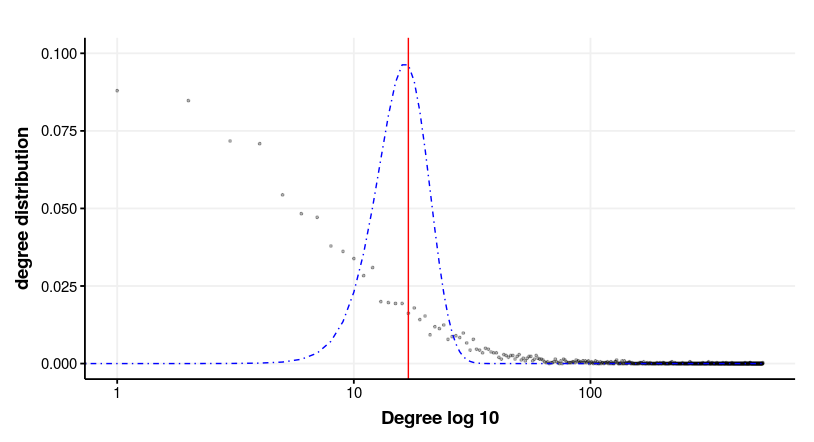
\includegraphics[width=\textwidth]{images/chapter3/ggplot2/theme/powerlaw/Rplot01_poissonanddegree2.png}
    \caption[Degree distribution with Poisson pdf overlaid]{Plot of degree distribution PSP with degree $k$ on x axis with log10 scaling. The degree distribution (the frequency of nodes of degree $k$ or $\frac{n_k}{k}$ is plotted on the y axis). The blue dash is the expected degree distribution given a Poisson distribution with mean equal to the mean of the empirical degree distribution. The solid vertical red line is the average degree. \url{source('~/RProjects/group_size_distribution/R/poissonanddegree_theme.R')}\textcolor{red}{check this is Expected value vs pdf}}
    \label{fig:PSP degree power-law poisson}
\end{figure}

\begin{figure}
    \centering
    \begin{subfigure}[t]{0.45\textwidth}
        \centering
        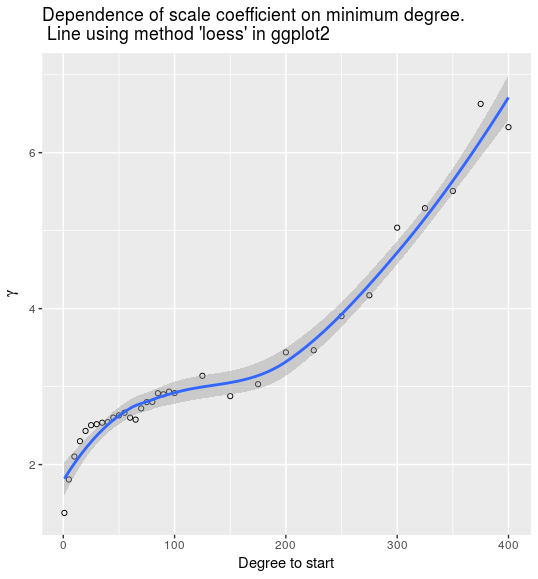
\includegraphics[width=\linewidth]{images/dependence_of_scale_coefficient_on_min_degree.png} 
        \caption{The parameter $\gamma$ as a function of the degree at which calculation of the coefficient starts in the degree sequence(e.g. all degree $>5$) from \url{RProjects/PhDGraphs/calculate/gamma}} \label{fig:gamma}
    \end{subfigure}
    \hfill
    \begin{subfigure}[t]{0.45\textwidth}
        \centering
        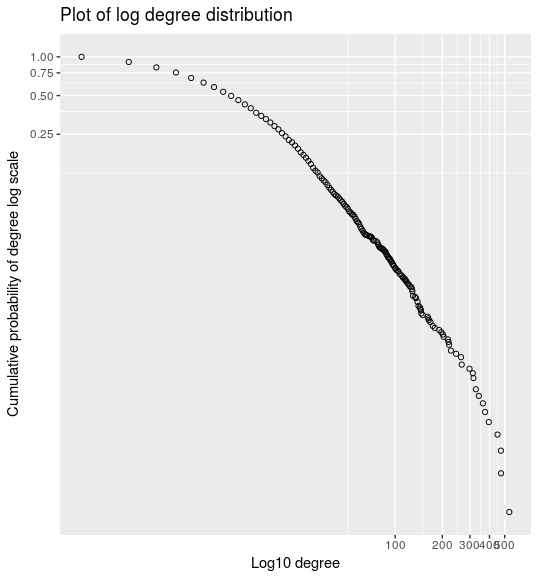
\includegraphics[width=\linewidth]{images/plot_log_degree_distribution.png} 
        \caption{The plot of log cumulative cdf of degree distribution log 10 scale x and y. \textcolor{red}{this is 1 -cdf Actually see Newman on cdf complement}} \label{fig:log_degree_distribution}
    \end{subfigure}
    \caption{Plots of degree distribution \textcolor{red}{may want to do this in subfigure packages rather than subcaption to line up edges}}
    \label{fig:Plots of degree distribution}
\end{figure}




\begin{table}[]
    \centering
    
    \begin{tabular}{ccccccc}
    \toprule
        Distribution & Log $L$ & bootstrap $p$ & $x_{min}$ & $\gamma$ or pars & Vuong $p$  &g.o.f.\\
        \midrule
        Power law \\
        Log-normal \\
        Exponential \\
        Poisson \\
    
  %      Weibull & -2925.3 &&& 0.230 ,0.0157 & drop weibull\\
        \bottomrule
    \end{tabular}
    \caption[Log $L$ of degree distribution under different models]{log-likelihood (Log $L$) of degree distribution under x min defined for power law. All distributions fitted from xmin of power law per Gillespie and Clauset etc. Vuong $p$ = one sided $p$ Vuong's closeness. g.o.f is Kolmogorov Smirnov distance statistic. *Need to recheck vuong as should be versus power law so not quoted with power law test\url{source('~/RProjects/chapter3/R/fit_power_law/fit_pl_setxmin.R')} }
    \tiny{Bootstrap p returns an error for Weibull and Weibull is a continuous distribution Error in checkForRemoteErrors(val) one node produced an error: non-finite finite-difference value [1] So we should probably drop the Weibull as it does not make comparisons easy and probably does not add very much to what we are saying which is can't choose between power law and log-normal}
    \label{tab:ll distributions}
\end{table}
\begin{table}[]
    \centering
    
    \begin{tabular}{ccccccc}
    \toprule
        Distribution & Log $L$ & bootstrap $p$ & $x_{min}$ & $\gamma$ or pars & Vuong $p$  &g.o.f.\\
        \midrule
        Power law &  -2943.6 & 0.575 & 24 & 2.51 & 0.906* &  0.0190\\
        Log-normal & -2941.6 & 0.4 (0.32) &&-2.34, 2.11& 0.903 &  0.01380035\\
        Exponential & -3044.7 & $<0.01$&&0.0285& $1.72\times10^{-7}$\\
        Poisson & -14376.3 & 0&&58.59 & & 0.088\\
    
  %      Weibull & -2925.3 &&& 0.230 ,0.0157 & drop weibull\\
        \bottomrule
    \end{tabular}
    \caption[Log $L$ of degree distribution under different models]{log-likelihood (Log $L$) of degree distribution under x min defined for power law. All distributions fitted from xmin of power law per Gillespie and Clauset etc. Vuong $p$ = one sided $p$ Vuong's closeness. g.o.f is Kolmogorov Smirnov distance statistic. *Need to recheck vuong as should be versus power law so not quoted with power law test\url{source('~/RProjects/chapter3/R/fit_power_law/fit_pl_setxmin.R')} }
    \tiny{Bootstrap p returns an error for Weibull and Weibull is a continuous distribution Error in checkForRemoteErrors(val) one node produced an error: non-finite finite-difference value [1] So we should probably drop the Weibull as it does not make comparisons easy and probably does not add very much to what we are saying which is can't choose between power law and log-normal}
    \label{tab:ll distributions}
\end{table}

\section{===to supplemental===}
  A table of the values of $\gamma$ for different values of $x_{min}$ can be found in supplementary table~\ref{table:gamma}.

\section{Extra figures}
\begin{figure} 
    \centering
    \includegraphics[width=\textwidth]{images/chapter3/cor_pairs/ggally/Rplot_corr_plot_ggally_large_size_11.png}
    \caption{Scatter plot of centrality measures. Transitivity where isolates set to zero omitted for clarity and space considerations. Spearman correlation in upper triangular. Source \url{source('~/RProjects/disgen2/R/cor/cor.R')}}
    \label{fig:scatter plot of multiple centralities gg ally}
\end{figure}
There is a broader dispersion of nodes from the trend line in where they are of high degree and the degree occurs only once in the degree sequence (figure~\ref{fig:Degree distribution of post synaptic proteome. Log10 - log10 scale.}).

\begin{figure}
    \includegraphics[width=12cm]{Rplot_DegreeDistribution}
    \caption{Degree distribution of post synaptic proteome. Log10 - log10 scale. Code at \url{source('~/RProjects/gridsearch_gamma/R/plot_log_degreedist.R') }}
    \label{fig:Degree distribution of post synaptic proteome. Log10 - log10 scale.}
\end{figure}



\subsection{C(k)}

\begin{figure}
    \centering
    \includegraphics[width=\textwidth]{images/chapter3/ggplot2/degree_and_transitivity/Rplot_scatterplot_c_and_degree_new_format.png}
      \caption{Scatter plot of the relationship between degree and local transitivity for the PSP nodes. Nodes with degree 1 have transitivity set to zero as transitivity in this case is undefined. Plot appears to show a negative correlation between degree and transitivity. The opacity of points has been decreased to reduce overplotting and show the increase in points at low degree. Potential replacement - \textcolor{red}{changed now} }
      \tiny\url{source('~/RProjects/chapter3/R/transitivity/transitivity_and_degree/mean_deg_seq.R')} plot p
    \label{fig:Scatter plot of the relationship between degree and local transitivity for the PSP nodes}
    
\end{figure}


\begin{figure}
    \centering
    \includegraphics[width=\textwidth]{images/chapter3/ggplot2/degree_and_transitivity/Rplot_rho_and_starting_degree_transitivity.png}
    \caption{Plot of minumum degree included in the calculation of Spearmans rank correlation between degree and $\rho$. Although the overall coefficient is positive the correlation for nodes above degree 5 are clearly negative and this becomes more apparent at high degree. This relationship is therefore complex and the typical relationship described in the literature may only hold for the large networks in which this relationship has been studies such as the internet}.
    \tiny\url{source('~/RProjects/chapter3/R/transitivity/transitivity_and_degree/plot/plot_start_degree.R')}
    \label{fig:Plot of minumum degree included in the calculation of Spearmans rank correlation between degree and rho}
\end{figure}



\subsection{DEG}

\begin{figure}
    \centering
    \includegraphics[width=\textwidth]{images/chapter3/ggplot2/db_essential_genes/theme/Rplot_single_boxplot_three_categories.png}
    \caption{Boxplot of the degree for genes in PSP and in database of essential genes(DEG). On the x axis are three groups: those genes that do not appear in the DEG, those with at least one entry but less than five and those with five or more. Y axis is log10 transform of vertex (node) degree. The graph shows degree increasing across the three categories as genes become more essential. Notch is $\frac{1.58 IQR}{\sqrt{n}}$}
    \tiny\url{source('~/RProjects/db_essential_genes/R/get_essential_genes/db_2020/plots/get_db_essential_threecategoriesboxplot_essential_centrality.R')}
    \label{fig:boxplot_three_groups_DEG_logdegree1}
\end{figure}




\begin{figure}
    \centering
    \includegraphics[width=\textwidth]{images/chapter3/ggplot2/db_essential_genes/theme/Rplot_multiplot_with_theme_simple.png}
    \caption{Multiple boxplot of the centrality measure for genes in PSP and in database of essential genes(DEG). On the x axis are three groups: those genes that do not appear in the DEG, those with at least one entry but less than five and those with five or more. Y axis is log10 transform of vertex (node) degree for degree, betweenness and eigenvector centrality. The graph shows degree increasing across the three categories as genes become more essential.} 
    \tiny\url{ source('~/RProjects/db_essential_genes/R/get_essential_genes/db_2020/theme/get_db_essential_threecategoriesboxplot_multiplot_no_x_lab_essential_centrality_theme.R')}
    \label{fig:boxplot_three_groups_DEG_multiplot1}
\end{figure}


\section{Extra tables}
% latex table generated in R 3.6.1 by xtable 1.8-4 package
% Sun Mar  7 16:19:10 2021
\begin{table}[ht]
\centering
\begin{adjustbox}{width = \textwidth}
\begin{tabular}{rrrrrrrr}
  \hline
 & degree & betweenness & eigenvector & closeness & transitivityNA & transitivity0 & kcoreness \\ 
  \hline
degree & 1.000 & 0.827 & 0.815 & 0.769 & -0.086 & -0.086 & 0.958 \\ 
  betweenness & 0.827 & 1.000 & 0.598 & 0.650 & -0.315 & -0.315 & 0.707 \\ 
  eigenvector & 0.815 & 0.598 & 1.000 & 0.938 & 0.174 & 0.174 & 0.881 \\ 
  closeness & 0.769 & 0.650 & 0.938 & 1.000 & 0.120 & 0.120 & 0.821 \\ 
  transitivityNA & -0.086 & -0.315 & 0.174 & 0.120 & 1.000 & 1.000 & 0.058 \\ 
  transitivity0 & -0.086 & -0.315 & 0.174 & 0.120 & 1.000 & 1.000 & 0.058 \\ 
  kcoreness & 0.958 & 0.707 & 0.881 & 0.821 & 0.058 & 0.058 & 1.000 \\ 
   \hline
\end{tabular}
\end{adjustbox}
\caption[Correlation of centrality measures for nodes $k>=5$]{Correlation of centrality measures. For nodes with degree five or more Spearman. Method for missing data include only pairwise complete. TransitivityNA treats isolates as NA and removes from calculation. Transitivity0 uses the option to set isolates to 0. Note that both measures of local transitivity are now identical and there is a clear negative correlation between betweenness and transitivity and between degree and transitivity.\url{source('~/RProjects/db_essential_genes/R/get_corr/cor_centrality_measures_ordered_cortable.R')}} 
\label{tab:Correlation of centrality measures 2 transitvities deg five or more}
\end{table}
\paragraph{Pearson}

% latex table generated in R 3.6.3 by xtable 1.8-4 package
% Sun Mar 28 14:53:37 2021
\begin{table}[ht]
\centering
\begin{tabular}{lrrrrrr}
  \toprule
Centrality & t & df & low & high & r & p \\ 
  \midrule
Degree & -0.136 & 3307 & -0.036 & 0.032 & -0.002 & 0.892 \\ 
  Betweenness & -0.412 & 3307 & -0.041 & 0.027 & -0.007 & 0.680 \\ 
  Eigenvector & -0.512 & 3307 & -0.043 & 0.025 & -0.009 & 0.608 \\ 
  Closeness & -0.785 & 3307 & -0.048 & 0.020 & -0.014 & 0.433 \\ 
  TransitivityNA & -0.880 & 3019 & -0.052 & 0.020 & -0.016 & 0.379 \\ 
  Transitivity0 & -0.680 & 3307 & -0.046 & 0.022 & -0.012 & 0.497 \\ 
  kcoreness & 0.380 & 3307 & -0.027 & 0.041 & 0.007 & 0.704 \\ 
   \bottomrule
\end{tabular}
\caption{Correlation of centrality measures with negative log 10 transform p Pearson IntelligenceReplication} 
\tiny\url{source('~/RProjects/chapter3/R/centrality_ch3/centrality_and_gwas_p_val/0_load_magma_pearson_centrality_ctg.R')}
\label{tab:Correlation of centrality measures with negative log 10 transform p Pearson IntelligenceReplication}
\end{table}

% latex table generated in R 3.6.3 by xtable 1.8-4 package
% Sun Mar 28 14:56:04 2021
\begin{table}[ht]
\centering
\begin{tabular}{lrrrrrr}
  \toprule
Centrality & t & df & low & high & r & p \\ 
  \midrule
Degree & 1.051 & 3283 & -0.016 & 0.052 & 0.018 & 0.293 \\ 
  Betweenness & 0.874 & 3283 & -0.019 & 0.049 & 0.015 & 0.382 \\ 
  Eigenvector & -0.054 & 3283 & -0.035 & 0.033 & -0.001 & 0.957 \\ 
  Closeness & -0.735 & 3283 & -0.047 & 0.021 & -0.013 & 0.462 \\ 
  TransitivityNA & -2.009 & 2998 & -0.072 & -0.001 & -0.037 & 0.045 \\ 
  Transitivity0 & -1.793 & 3283 & -0.065 & 0.003 & -0.031 & 0.073 \\ 
  kcoreness & -0.372 & 3283 & -0.041 & 0.028 & -0.006 & 0.710 \\ 
   \bottomrule
\end{tabular}
\caption{Correlation of centrality measures with negative log 10 transform p Pearson EducationReplication} 
\tiny\url{source('~/RProjects/chapter3/R/centrality_ch3/centrality_and_gwas_p_val/0_load_magma_pearson_centrality_ea2.R')}
\label{tab:Correlation of centrality measures with negative log 10 transform p Pearson EducationReplication}
\end{table}



% latex table generated in R 3.6.3 by xtable 1.8-4 package
% Sun Mar 28 14:57:24 2021
\begin{table}[ht]
\centering
\begin{tabular}{lrrrrrr}
  \toprule
Centrality & t & df & low & high & r & p \\ 
  \midrule
Degree & -0.836 & 3299 & -0.049 & 0.020 & -0.015 & 0.403 \\ 
  Betweenness & -0.549 & 3299 & -0.044 & 0.025 & -0.010 & 0.583 \\ 
  Eigenvector & -1.740 & 3299 & -0.064 & 0.004 & -0.030 & 0.082 \\ 
  Closeness & -1.634 & 3299 & -0.062 & 0.006 & -0.028 & 0.102 \\ 
  TransitivityNA & 0.741 & 3012 & -0.022 & 0.049 & 0.013 & 0.459 \\ 
  Transitivity0 & 0.862 & 3299 & -0.019 & 0.049 & 0.015 & 0.389 \\ 
  kcoreness & -1.000 & 3299 & -0.051 & 0.017 & -0.017 & 0.317 \\ 
   \bottomrule
\end{tabular}
\caption{Correlation of centrality measures with negative log 10 transform p Pearson EducationDiscovery} 
\tiny\url{source('~/RProjects/chapter3/R/centrality_ch3/centrality_and_gwas_p_val/0_load_magma_pearson_centrality_ukbbed.R')}
\label{tab:Correlation of centrality measures with negative log 10 transform p Pearson EducationDiscovery}
\end{table}



% latex table generated in R 3.6.3 by xtable 1.8-4 package
% Sun Mar 28 14:58:36 2021
\begin{table}[ht]
\centering
\begin{tabular}{lrrrrrr}
  \toprule
Centrality & t & df & low & high & r & p \\ 
  \midrule
Degree & -0.396 & 3299 & -0.041 & 0.027 & -0.007 & 0.692 \\ 
  Betweenness & 0.039 & 3299 & -0.033 & 0.035 & 0.001 & 0.969 \\ 
  Eigenvector & -0.310 & 3299 & -0.039 & 0.029 & -0.005 & 0.757 \\ 
  Closeness & -1.311 & 3299 & -0.057 & 0.011 & -0.023 & 0.190 \\ 
  TransitivityNA & 0.587 & 3012 & -0.025 & 0.046 & 0.011 & 0.557 \\ 
  Transitivity0 & 0.685 & 3299 & -0.022 & 0.046 & 0.012 & 0.493 \\ 
  kcoreness & -1.480 & 3299 & -0.060 & 0.008 & -0.026 & 0.139 \\ 
   \bottomrule
\end{tabular}
\caption{Correlation of centrality measures with negative log 10 transform p Pearson IntelligenceDiscovery} 
\tiny\url{source('~/RProjects/chapter3/R/centrality_ch3/centrality_and_gwas_p_val/0_load_magma_pearson_centrality_ukbb_int.R')}
\label{tab:Correlation of centrality measures with negative log 10 transform p Pearson IntelligenceDiscovery}
\end{table}
%\begin{figure}]h]
%  \includegraphics[width=\linewidth]{Rplot_transitivity}
%  \caption{Transitivity}
%  \label{fig:transitivity}
%\end{figure}
 
%\begin{figure}]h]
%  \includegraphics[width=\linewidth]{Rplot_transitivity_degree}
%  \caption{Local clustering coefficient and degree}
%  \label{fig:transitivity_degree}
%\end{figure}


%\begin{figure}
%    \centering
%    \includegraphics[width=\linewidth]{images/Rplot01_logdegree_log_transitivity.png}
%    \caption{Plot of degree with mean local transitivity. Log10-log10 scale. Omitting degree $k=1$ as transitivity $C$ will be undefined.}
 %   \label{fig:log_transitivity_degree}
%\end{figure}
\subsubsection{Compare diseases}

ALS Mean degree 50.62
PD Mean deg 30.26


Curated diseases for Picks 2 genes BeFree (text mining) 210

I guess the fact that the text mined data is similar in centrality to those of other neurdegenerative is in support


ID 412 in PSP 1219 in middle in centrality 

FTD 119 PSP 304 total  high centrality BeFree

ASD higher degree similar eigenvector 300 PSP 1018 total

Epilespy slightly higher PSP 380 All 1124 ? the low tail is enriched for epilepsy

BPD Similar to PSP 863 total 240 in PSP

SCZ be free 2217 PSP 623 Similar eigenvector higher betweenness

Depression slightly up degree lower eig 1416 genes 340 in PSP

Neuroticism 141 28 in PSP
Degree similar eig lower core

Cognitive dysfunction slightly higher deg and eig 1368 415 in PSP

OCD almost identical 166 genes 45 in PSP

Neurodegen double degree and betweenness similar eig 484 in PSP 1480 total

Neurodevelopmental - double bet, similar eig, about 10 higher deg

Psychotic - almost identical all 125 PSP 438 total

Borderline - higher degree 3x betweenness similar eig and coreness 220 PSP 56

Antisocial PSP 14 all 63
2x degree 3x between

Huntingdon 945 271 in PSD 
Deg almost double 3 x bet 2 x eig  increase kcore 3

Encephalitis
4 x bet double deg not much change eig 68 PSP 285 curated 

\url{source('~/RProjects/disgen2/R/disgen/specific_disorders/summaries_curated/encephalitis.R')}

\todo{you could angle this as similar to the cognitive based disorders etc in Pocklington}



\todo{We get ngenes and nspns so map snps to genes}